\documentclass[twoside]{book}

% Packages required by doxygen
\usepackage{fixltx2e}
\usepackage{calc}
\usepackage{doxygen}
\usepackage[export]{adjustbox} % also loads graphicx
\usepackage{graphicx}
\usepackage[utf8]{inputenc}
\usepackage{makeidx}
\usepackage{multicol}
\usepackage{multirow}
\PassOptionsToPackage{warn}{textcomp}
\usepackage{textcomp}
\usepackage[nointegrals]{wasysym}
\usepackage[table]{xcolor}

% Font selection
\usepackage[T1]{fontenc}
\usepackage[scaled=.90]{helvet}
\usepackage{courier}
\usepackage{amssymb}
\usepackage{sectsty}
\renewcommand{\familydefault}{\sfdefault}
\allsectionsfont{%
  \fontseries{bc}\selectfont%
  \color{darkgray}%
}
\renewcommand{\DoxyLabelFont}{%
  \fontseries{bc}\selectfont%
  \color{darkgray}%
}
\newcommand{\+}{\discretionary{\mbox{\scriptsize$\hookleftarrow$}}{}{}}

% Page & text layout
\usepackage{geometry}
\geometry{%
  a4paper,%
  top=2.5cm,%
  bottom=2.5cm,%
  left=2.5cm,%
  right=2.5cm%
}
\tolerance=750
\hfuzz=15pt
\hbadness=750
\setlength{\emergencystretch}{15pt}
\setlength{\parindent}{0cm}
\setlength{\parskip}{3ex plus 2ex minus 2ex}
\makeatletter
\renewcommand{\paragraph}{%
  \@startsection{paragraph}{4}{0ex}{-1.0ex}{1.0ex}{%
    \normalfont\normalsize\bfseries\SS@parafont%
  }%
}
\renewcommand{\subparagraph}{%
  \@startsection{subparagraph}{5}{0ex}{-1.0ex}{1.0ex}{%
    \normalfont\normalsize\bfseries\SS@subparafont%
  }%
}
\makeatother

% Headers & footers
\usepackage{fancyhdr}
\pagestyle{fancyplain}
\fancyhead[LE]{\fancyplain{}{\bfseries\thepage}}
\fancyhead[CE]{\fancyplain{}{}}
\fancyhead[RE]{\fancyplain{}{\bfseries\leftmark}}
\fancyhead[LO]{\fancyplain{}{\bfseries\rightmark}}
\fancyhead[CO]{\fancyplain{}{}}
\fancyhead[RO]{\fancyplain{}{\bfseries\thepage}}
\fancyfoot[LE]{\fancyplain{}{}}
\fancyfoot[CE]{\fancyplain{}{}}
\fancyfoot[RE]{\fancyplain{}{\bfseries\scriptsize Generated by Doxygen }}
\fancyfoot[LO]{\fancyplain{}{\bfseries\scriptsize Generated by Doxygen }}
\fancyfoot[CO]{\fancyplain{}{}}
\fancyfoot[RO]{\fancyplain{}{}}
\renewcommand{\footrulewidth}{0.4pt}
\renewcommand{\chaptermark}[1]{%
  \markboth{#1}{}%
}
\renewcommand{\sectionmark}[1]{%
  \markright{\thesection\ #1}%
}

% Indices & bibliography
\usepackage{natbib}
\usepackage[titles]{tocloft}
\setcounter{tocdepth}{3}
\setcounter{secnumdepth}{5}
\makeindex

% Hyperlinks (required, but should be loaded last)
\usepackage{ifpdf}
\ifpdf
  \usepackage[pdftex,pagebackref=true]{hyperref}
\else
  \usepackage[ps2pdf,pagebackref=true]{hyperref}
\fi
\hypersetup{%
  colorlinks=true,%
  linkcolor=blue,%
  citecolor=blue,%
  unicode%
}

% Custom commands
\newcommand{\clearemptydoublepage}{%
  \newpage{\pagestyle{empty}\cleardoublepage}%
}

\usepackage{caption}
\captionsetup{labelsep=space,justification=centering,font={bf},singlelinecheck=off,skip=4pt,position=top}

%===== C O N T E N T S =====

\begin{document}

% Titlepage & ToC
\hypersetup{pageanchor=false,
             bookmarksnumbered=true,
             pdfencoding=unicode
            }
\pagenumbering{alph}
\begin{titlepage}
\vspace*{7cm}
\begin{center}%
{\Large My Project }\\
\vspace*{1cm}
{\large Generated by Doxygen 1.8.13}\\
\end{center}
\end{titlepage}
\clearemptydoublepage
\pagenumbering{roman}
\tableofcontents
\clearemptydoublepage
\pagenumbering{arabic}
\hypersetup{pageanchor=true}

%--- Begin generated contents ---
\chapter{Bug List}
\label{bug}
\Hypertarget{bug}

\begin{DoxyRefList}
\item[\label{bug__bug000001}%
\Hypertarget{bug__bug000001}%
Member \hyperlink{class_text_box_a19cb5e85c864060ecdb2fe2bab6fd54d}{Text\+Box\+:\+:create\+Strings} (std\+::string text, T\+T\+F\+\_\+\+Font $\ast$font)]There is currently an issue where the texture will return 0, temp fix has been implemented where the texture width is hardcoded 
\end{DoxyRefList}
\chapter{Namespace Index}
\section{Namespace List}
Here is a list of all namespaces with brief descriptions\+:\begin{DoxyCompactList}
\item\contentsline{section}{\hyperlink{namespacecomments}{comments} }{\pageref{namespacecomments}}{}
\end{DoxyCompactList}

\chapter{Hierarchical Index}
\section{Class Hierarchy}
This inheritance list is sorted roughly, but not completely, alphabetically\+:\begin{DoxyCompactList}
\item \contentsline{section}{Base\+\_\+\+Group}{\pageref{class_base___group}}{}
\begin{DoxyCompactList}
\item \contentsline{section}{N\+P\+C\+\_\+\+Group}{\pageref{class_n_p_c___group}}{}
\item \contentsline{section}{User\+\_\+\+Group}{\pageref{class_user___group}}{}
\end{DoxyCompactList}
\item \contentsline{section}{Comment}{\pageref{class_comment}}{}
\item \contentsline{section}{Comment\+Formatter}{\pageref{class_comment_formatter}}{}
\item \contentsline{section}{Group}{\pageref{class_group}}{}
\item \contentsline{section}{Group\+Populator}{\pageref{class_group_populator}}{}
\item \contentsline{section}{J\+S\+O\+N\+Reader}{\pageref{class_j_s_o_n_reader}}{}
\item \contentsline{section}{Node}{\pageref{class_node}}{}
\item \contentsline{section}{comments.\+Object}{\pageref{classcomments_1_1_object}}{}
\item \contentsline{section}{Python\+Handler}{\pageref{class_python_handler}}{}
\item \contentsline{section}{Resource\+Data}{\pageref{class_resource_data}}{}
\item \contentsline{section}{Room}{\pageref{class_room}}{}
\item \contentsline{section}{S\+D\+L\+Window}{\pageref{class_s_d_l_window}}{}
\item \contentsline{section}{Sprite}{\pageref{class_sprite}}{}
\begin{DoxyCompactList}
\item \contentsline{section}{N\+PC}{\pageref{class_n_p_c}}{}
\item \contentsline{section}{Text\+Box}{\pageref{class_text_box}}{}
\end{DoxyCompactList}
\item \contentsline{section}{Texture}{\pageref{class_texture}}{}
\item \contentsline{section}{Topic}{\pageref{class_topic}}{}
\end{DoxyCompactList}

\chapter{Class Index}
\section{Class List}
Here are the classes, structs, unions and interfaces with brief descriptions\+:\begin{DoxyCompactList}
\item\contentsline{section}{\hyperlink{class_base___group}{Base\+\_\+\+Group} }{\pageref{class_base___group}}{}
\item\contentsline{section}{\hyperlink{class_comment}{Comment} }{\pageref{class_comment}}{}
\item\contentsline{section}{\hyperlink{class_comment_formatter}{Comment\+Formatter} }{\pageref{class_comment_formatter}}{}
\item\contentsline{section}{\hyperlink{class_group}{Group} }{\pageref{class_group}}{}
\item\contentsline{section}{\hyperlink{class_group_populator}{Group\+Populator} }{\pageref{class_group_populator}}{}
\item\contentsline{section}{\hyperlink{class_j_s_o_n_reader}{J\+S\+O\+N\+Reader} }{\pageref{class_j_s_o_n_reader}}{}
\item\contentsline{section}{\hyperlink{class_node}{Node} }{\pageref{class_node}}{}
\item\contentsline{section}{\hyperlink{class_n_p_c}{N\+PC} }{\pageref{class_n_p_c}}{}
\item\contentsline{section}{\hyperlink{class_n_p_c___group}{N\+P\+C\+\_\+\+Group} }{\pageref{class_n_p_c___group}}{}
\item\contentsline{section}{\hyperlink{classcomments_1_1_object}{comments.\+Object} }{\pageref{classcomments_1_1_object}}{}
\item\contentsline{section}{\hyperlink{class_python_handler}{Python\+Handler} }{\pageref{class_python_handler}}{}
\item\contentsline{section}{\hyperlink{class_resource_data}{Resource\+Data} }{\pageref{class_resource_data}}{}
\item\contentsline{section}{\hyperlink{class_room}{Room} }{\pageref{class_room}}{}
\item\contentsline{section}{\hyperlink{class_s_d_l_window}{S\+D\+L\+Window} }{\pageref{class_s_d_l_window}}{}
\item\contentsline{section}{\hyperlink{class_sprite}{Sprite} }{\pageref{class_sprite}}{}
\item\contentsline{section}{\hyperlink{class_text_box}{Text\+Box} }{\pageref{class_text_box}}{}
\item\contentsline{section}{\hyperlink{class_texture}{Texture} }{\pageref{class_texture}}{}
\item\contentsline{section}{\hyperlink{class_topic}{Topic} }{\pageref{class_topic}}{}
\item\contentsline{section}{\hyperlink{class_user___group}{User\+\_\+\+Group} }{\pageref{class_user___group}}{}
\end{DoxyCompactList}

\chapter{File Index}
\section{File List}
Here is a list of all files with brief descriptions\+:\begin{DoxyCompactList}
\item\contentsline{section}{C\+:/\+Users/\+Kyle Tuckey/\+Documents/\+Final Year Project/\+Social\+\_\+\+N\+P\+C\+S/\+Social\+\_\+\+N\+P\+C\+S/\hyperlink{_base___group_8cpp}{Base\+\_\+\+Group.\+cpp} \\*Base class for the \hyperlink{class_n_p_c}{N\+PC} group classes The \hyperlink{class_n_p_c___group}{N\+P\+C\+\_\+\+Group} class is designed to represent a maximum group of 6 \hyperlink{class_n_p_c}{N\+PC}\textquotesingle{}s. the specfied \hyperlink{class_n_p_c}{N\+PC}\textquotesingle{}s are initialised when the group is initialised }{\pageref{_base___group_8cpp}}{}
\item\contentsline{section}{C\+:/\+Users/\+Kyle Tuckey/\+Documents/\+Final Year Project/\+Social\+\_\+\+N\+P\+C\+S/\+Social\+\_\+\+N\+P\+C\+S/\hyperlink{_base___group_8h}{Base\+\_\+\+Group.\+h} }{\pageref{_base___group_8h}}{}
\item\contentsline{section}{C\+:/\+Users/\+Kyle Tuckey/\+Documents/\+Final Year Project/\+Social\+\_\+\+N\+P\+C\+S/\+Social\+\_\+\+N\+P\+C\+S/\hyperlink{_comment_8cpp}{Comment.\+cpp} }{\pageref{_comment_8cpp}}{}
\item\contentsline{section}{C\+:/\+Users/\+Kyle Tuckey/\+Documents/\+Final Year Project/\+Social\+\_\+\+N\+P\+C\+S/\+Social\+\_\+\+N\+P\+C\+S/\hyperlink{_comment_8h}{Comment.\+h} }{\pageref{_comment_8h}}{}
\item\contentsline{section}{C\+:/\+Users/\+Kyle Tuckey/\+Documents/\+Final Year Project/\+Social\+\_\+\+N\+P\+C\+S/\+Social\+\_\+\+N\+P\+C\+S/\hyperlink{_comment_formatter_8cpp}{Comment\+Formatter.\+cpp} }{\pageref{_comment_formatter_8cpp}}{}
\item\contentsline{section}{C\+:/\+Users/\+Kyle Tuckey/\+Documents/\+Final Year Project/\+Social\+\_\+\+N\+P\+C\+S/\+Social\+\_\+\+N\+P\+C\+S/\hyperlink{_comment_formatter_8h}{Comment\+Formatter.\+h} }{\pageref{_comment_formatter_8h}}{}
\item\contentsline{section}{C\+:/\+Users/\+Kyle Tuckey/\+Documents/\+Final Year Project/\+Social\+\_\+\+N\+P\+C\+S/\+Social\+\_\+\+N\+P\+C\+S/\hyperlink{comments_8py}{comments.\+py} }{\pageref{comments_8py}}{}
\item\contentsline{section}{C\+:/\+Users/\+Kyle Tuckey/\+Documents/\+Final Year Project/\+Social\+\_\+\+N\+P\+C\+S/\+Social\+\_\+\+N\+P\+C\+S/\hyperlink{_group_8cpp}{Group.\+cpp} }{\pageref{_group_8cpp}}{}
\item\contentsline{section}{C\+:/\+Users/\+Kyle Tuckey/\+Documents/\+Final Year Project/\+Social\+\_\+\+N\+P\+C\+S/\+Social\+\_\+\+N\+P\+C\+S/\hyperlink{_group_8h}{Group.\+h} }{\pageref{_group_8h}}{}
\item\contentsline{section}{C\+:/\+Users/\+Kyle Tuckey/\+Documents/\+Final Year Project/\+Social\+\_\+\+N\+P\+C\+S/\+Social\+\_\+\+N\+P\+C\+S/\hyperlink{_group_populator_8cpp}{Group\+Populator.\+cpp} }{\pageref{_group_populator_8cpp}}{}
\item\contentsline{section}{C\+:/\+Users/\+Kyle Tuckey/\+Documents/\+Final Year Project/\+Social\+\_\+\+N\+P\+C\+S/\+Social\+\_\+\+N\+P\+C\+S/\hyperlink{_group_populator_8h}{Group\+Populator.\+h} }{\pageref{_group_populator_8h}}{}
\item\contentsline{section}{C\+:/\+Users/\+Kyle Tuckey/\+Documents/\+Final Year Project/\+Social\+\_\+\+N\+P\+C\+S/\+Social\+\_\+\+N\+P\+C\+S/\hyperlink{_j_s_o_n_reader_8cpp}{J\+S\+O\+N\+Reader.\+cpp} }{\pageref{_j_s_o_n_reader_8cpp}}{}
\item\contentsline{section}{C\+:/\+Users/\+Kyle Tuckey/\+Documents/\+Final Year Project/\+Social\+\_\+\+N\+P\+C\+S/\+Social\+\_\+\+N\+P\+C\+S/\hyperlink{_j_s_o_n_reader_8h}{J\+S\+O\+N\+Reader.\+h} }{\pageref{_j_s_o_n_reader_8h}}{}
\item\contentsline{section}{C\+:/\+Users/\+Kyle Tuckey/\+Documents/\+Final Year Project/\+Social\+\_\+\+N\+P\+C\+S/\+Social\+\_\+\+N\+P\+C\+S/\hyperlink{_node_8cpp}{Node.\+cpp} }{\pageref{_node_8cpp}}{}
\item\contentsline{section}{C\+:/\+Users/\+Kyle Tuckey/\+Documents/\+Final Year Project/\+Social\+\_\+\+N\+P\+C\+S/\+Social\+\_\+\+N\+P\+C\+S/\hyperlink{_node_8h}{Node.\+h} }{\pageref{_node_8h}}{}
\item\contentsline{section}{C\+:/\+Users/\+Kyle Tuckey/\+Documents/\+Final Year Project/\+Social\+\_\+\+N\+P\+C\+S/\+Social\+\_\+\+N\+P\+C\+S/\hyperlink{_n_p_c_8cpp}{N\+P\+C.\+cpp} }{\pageref{_n_p_c_8cpp}}{}
\item\contentsline{section}{C\+:/\+Users/\+Kyle Tuckey/\+Documents/\+Final Year Project/\+Social\+\_\+\+N\+P\+C\+S/\+Social\+\_\+\+N\+P\+C\+S/\hyperlink{_n_p_c_8h}{N\+P\+C.\+h} }{\pageref{_n_p_c_8h}}{}
\item\contentsline{section}{C\+:/\+Users/\+Kyle Tuckey/\+Documents/\+Final Year Project/\+Social\+\_\+\+N\+P\+C\+S/\+Social\+\_\+\+N\+P\+C\+S/\hyperlink{_n_p_c___group_8cpp}{N\+P\+C\+\_\+\+Group.\+cpp} }{\pageref{_n_p_c___group_8cpp}}{}
\item\contentsline{section}{C\+:/\+Users/\+Kyle Tuckey/\+Documents/\+Final Year Project/\+Social\+\_\+\+N\+P\+C\+S/\+Social\+\_\+\+N\+P\+C\+S/\hyperlink{_n_p_c___group_8h}{N\+P\+C\+\_\+\+Group.\+h} }{\pageref{_n_p_c___group_8h}}{}
\item\contentsline{section}{C\+:/\+Users/\+Kyle Tuckey/\+Documents/\+Final Year Project/\+Social\+\_\+\+N\+P\+C\+S/\+Social\+\_\+\+N\+P\+C\+S/\hyperlink{_python_handler_8cpp}{Python\+Handler.\+cpp} }{\pageref{_python_handler_8cpp}}{}
\item\contentsline{section}{C\+:/\+Users/\+Kyle Tuckey/\+Documents/\+Final Year Project/\+Social\+\_\+\+N\+P\+C\+S/\+Social\+\_\+\+N\+P\+C\+S/\hyperlink{_python_handler_8h}{Python\+Handler.\+h} }{\pageref{_python_handler_8h}}{}
\item\contentsline{section}{C\+:/\+Users/\+Kyle Tuckey/\+Documents/\+Final Year Project/\+Social\+\_\+\+N\+P\+C\+S/\+Social\+\_\+\+N\+P\+C\+S/\hyperlink{_resource_data_8cpp}{Resource\+Data.\+cpp} }{\pageref{_resource_data_8cpp}}{}
\item\contentsline{section}{C\+:/\+Users/\+Kyle Tuckey/\+Documents/\+Final Year Project/\+Social\+\_\+\+N\+P\+C\+S/\+Social\+\_\+\+N\+P\+C\+S/\hyperlink{_resource_data_8h}{Resource\+Data.\+h} }{\pageref{_resource_data_8h}}{}
\item\contentsline{section}{C\+:/\+Users/\+Kyle Tuckey/\+Documents/\+Final Year Project/\+Social\+\_\+\+N\+P\+C\+S/\+Social\+\_\+\+N\+P\+C\+S/\hyperlink{_room_8cpp}{Room.\+cpp} }{\pageref{_room_8cpp}}{}
\item\contentsline{section}{C\+:/\+Users/\+Kyle Tuckey/\+Documents/\+Final Year Project/\+Social\+\_\+\+N\+P\+C\+S/\+Social\+\_\+\+N\+P\+C\+S/\hyperlink{_room_8h}{Room.\+h} }{\pageref{_room_8h}}{}
\item\contentsline{section}{C\+:/\+Users/\+Kyle Tuckey/\+Documents/\+Final Year Project/\+Social\+\_\+\+N\+P\+C\+S/\+Social\+\_\+\+N\+P\+C\+S/\hyperlink{_s_d_l_window_8cpp}{S\+D\+L\+Window.\+cpp} }{\pageref{_s_d_l_window_8cpp}}{}
\item\contentsline{section}{C\+:/\+Users/\+Kyle Tuckey/\+Documents/\+Final Year Project/\+Social\+\_\+\+N\+P\+C\+S/\+Social\+\_\+\+N\+P\+C\+S/\hyperlink{_s_d_l_window_8h}{S\+D\+L\+Window.\+h} }{\pageref{_s_d_l_window_8h}}{}
\item\contentsline{section}{C\+:/\+Users/\+Kyle Tuckey/\+Documents/\+Final Year Project/\+Social\+\_\+\+N\+P\+C\+S/\+Social\+\_\+\+N\+P\+C\+S/\hyperlink{_social___n_p_c_s_8cpp}{Social\+\_\+\+N\+P\+C\+S.\+cpp} }{\pageref{_social___n_p_c_s_8cpp}}{}
\item\contentsline{section}{C\+:/\+Users/\+Kyle Tuckey/\+Documents/\+Final Year Project/\+Social\+\_\+\+N\+P\+C\+S/\+Social\+\_\+\+N\+P\+C\+S/\hyperlink{_sprite_8cpp}{Sprite.\+cpp} }{\pageref{_sprite_8cpp}}{}
\item\contentsline{section}{C\+:/\+Users/\+Kyle Tuckey/\+Documents/\+Final Year Project/\+Social\+\_\+\+N\+P\+C\+S/\+Social\+\_\+\+N\+P\+C\+S/\hyperlink{_sprite_8h}{Sprite.\+h} }{\pageref{_sprite_8h}}{}
\item\contentsline{section}{C\+:/\+Users/\+Kyle Tuckey/\+Documents/\+Final Year Project/\+Social\+\_\+\+N\+P\+C\+S/\+Social\+\_\+\+N\+P\+C\+S/\hyperlink{targetver_8h}{targetver.\+h} }{\pageref{targetver_8h}}{}
\item\contentsline{section}{C\+:/\+Users/\+Kyle Tuckey/\+Documents/\+Final Year Project/\+Social\+\_\+\+N\+P\+C\+S/\+Social\+\_\+\+N\+P\+C\+S/\hyperlink{_text_box_8cpp}{Text\+Box.\+cpp} }{\pageref{_text_box_8cpp}}{}
\item\contentsline{section}{C\+:/\+Users/\+Kyle Tuckey/\+Documents/\+Final Year Project/\+Social\+\_\+\+N\+P\+C\+S/\+Social\+\_\+\+N\+P\+C\+S/\hyperlink{_text_box_8h}{Text\+Box.\+h} }{\pageref{_text_box_8h}}{}
\item\contentsline{section}{C\+:/\+Users/\+Kyle Tuckey/\+Documents/\+Final Year Project/\+Social\+\_\+\+N\+P\+C\+S/\+Social\+\_\+\+N\+P\+C\+S/\hyperlink{_texture_8cpp}{Texture.\+cpp} }{\pageref{_texture_8cpp}}{}
\item\contentsline{section}{C\+:/\+Users/\+Kyle Tuckey/\+Documents/\+Final Year Project/\+Social\+\_\+\+N\+P\+C\+S/\+Social\+\_\+\+N\+P\+C\+S/\hyperlink{_texture_8h}{Texture.\+h} }{\pageref{_texture_8h}}{}
\item\contentsline{section}{C\+:/\+Users/\+Kyle Tuckey/\+Documents/\+Final Year Project/\+Social\+\_\+\+N\+P\+C\+S/\+Social\+\_\+\+N\+P\+C\+S/\hyperlink{_topic_8cpp}{Topic.\+cpp} }{\pageref{_topic_8cpp}}{}
\item\contentsline{section}{C\+:/\+Users/\+Kyle Tuckey/\+Documents/\+Final Year Project/\+Social\+\_\+\+N\+P\+C\+S/\+Social\+\_\+\+N\+P\+C\+S/\hyperlink{_topic_8h}{Topic.\+h} }{\pageref{_topic_8h}}{}
\item\contentsline{section}{C\+:/\+Users/\+Kyle Tuckey/\+Documents/\+Final Year Project/\+Social\+\_\+\+N\+P\+C\+S/\+Social\+\_\+\+N\+P\+C\+S/\hyperlink{_user___group_8cpp}{User\+\_\+\+Group.\+cpp} }{\pageref{_user___group_8cpp}}{}
\item\contentsline{section}{C\+:/\+Users/\+Kyle Tuckey/\+Documents/\+Final Year Project/\+Social\+\_\+\+N\+P\+C\+S/\+Social\+\_\+\+N\+P\+C\+S/\hyperlink{_user___group_8h}{User\+\_\+\+Group.\+h} }{\pageref{_user___group_8h}}{}
\end{DoxyCompactList}

\chapter{Namespace Documentation}
\hypertarget{namespacecomments}{}\section{comments Namespace Reference}
\label{namespacecomments}\index{comments@{comments}}
\subsection*{Classes}
\begin{DoxyCompactItemize}
\item 
class \hyperlink{classcomments_1_1_object}{Object}
\end{DoxyCompactItemize}
\subsection*{Functions}
\begin{DoxyCompactItemize}
\item 
def \hyperlink{namespacecomments_a15146b34dd7b539d081e27278c3c322e}{get\+Sentiment} (body)
\item 
def \hyperlink{namespacecomments_aadd79f53e655498635ea6597a88b219c}{get\+Comments} ()
\end{DoxyCompactItemize}


\subsection{Function Documentation}
\mbox{\Hypertarget{namespacecomments_aadd79f53e655498635ea6597a88b219c}\label{namespacecomments_aadd79f53e655498635ea6597a88b219c}} 
\index{comments@{comments}!get\+Comments@{get\+Comments}}
\index{get\+Comments@{get\+Comments}!comments@{comments}}
\subsubsection{\texorpdfstring{get\+Comments()}{getComments()}}
{\footnotesize\ttfamily def comments.\+get\+Comments (\begin{DoxyParamCaption}{ }\end{DoxyParamCaption})}



Definition at line 27 of file comments.\+py.



References get\+Sentiment().


\begin{DoxyCode}
27 \textcolor{keyword}{def }\hyperlink{namespacecomments_aadd79f53e655498635ea6597a88b219c}{getComments}():
28     with open(\textcolor{stringliteral}{"ResourceData.json"}) \textcolor{keyword}{as} data\_file:
29         data = json.load(data\_file)
30     r = praw.Reddit(user\_agent = data[\textcolor{stringliteral}{"User\_Agent"}], client\_id= data[\textcolor{stringliteral}{"Client\_Id"}], client\_secret=data[\textcolor{stringliteral}{"
      Client\_Secret"}])
31     sub = r.subreddit(data[\textcolor{stringliteral}{"Sub\_Reddit"}])
32     subName = sub.fullname
33     d = Object()
34     d.subject = subName
35     d.topics = []
36     print(\textcolor{stringliteral}{"retrieving submissions"})
37     
38     \textcolor{comment}{#iterate over each submission}
39     counter = 0
40     i = 1;
41     \textcolor{keywordflow}{for} submission \textcolor{keywordflow}{in} sub.top(limit=5, time\_filter=\textcolor{stringliteral}{'day'}):
42         counter = counter + 1
43         submission.comments.replace\_more(limit=0)   
44         cList = []
45         rList = []  
46         comment\_queue = submission.comments[:]
47         top = Object()
48         top.topic = submission.title
49         top.id = submission.fullname
50 
51         \textcolor{keywordflow}{while} comment\_queue:
52             comment = comment\_queue.pop(0)
53             \textcolor{keywordflow}{if} comment.author != \textcolor{keywordtype}{None}:
54                 con = Object()
55                 con.id = comment.id
56                 con.body = re.sub(\textcolor{stringliteral}{' +'},\textcolor{stringliteral}{' '},comment.body.replace(\textcolor{stringliteral}{'\(\backslash\)n'}, \textcolor{stringliteral}{' '}).replace(\textcolor{stringliteral}{'\(\backslash\)r'},\textcolor{stringliteral}{' '}))
57                 con.polarity = \hyperlink{namespacecomments_a15146b34dd7b539d081e27278c3c322e}{getSentiment}(con.body)
58                 con.parent\_id = comment.parent\_id
59                 author = comment.author
60                 \textcolor{keywordflow}{if} author != \textcolor{keywordtype}{None}:
61                     con.author = author.name
62                 \textcolor{keywordflow}{else}:
63                     con.author = \textcolor{stringliteral}{"none"}
64                 \textcolor{comment}{#con.user = author.fullname}
65                 \textcolor{keywordflow}{if} i == 1:
66                     print(author.name)
67                     i = 0
68                 \textcolor{keywordflow}{if} comment.parent\_id == submission.fullname:
69                     con.reply = \textcolor{keyword}{False}
70                 \textcolor{keywordflow}{else}:
71                     con.reply = \textcolor{keyword}{True}
72                 cList.append(con)
73                 comment\_queue.extend(comment.replies)
74     
75         \textcolor{comment}{#iterate over each comment in the comment list}
76         top.comments = cList
77         d.topics.append(top)
78         print(\textcolor{stringliteral}{"\(\backslash\)rGenerated Objects : "} + str(counter))
79         
80     print(\textcolor{stringliteral}{"Generating JSON file"})
81     with open(\textcolor{stringliteral}{'data.json'}, \textcolor{stringliteral}{'w'}) \textcolor{keyword}{as} outfile:
82         outfile.write(d.toJSON())
83         outfile.close()
84 
85 \hyperlink{namespacecomments_aadd79f53e655498635ea6597a88b219c}{getComments}()
86 \end{DoxyCode}
\mbox{\Hypertarget{namespacecomments_a15146b34dd7b539d081e27278c3c322e}\label{namespacecomments_a15146b34dd7b539d081e27278c3c322e}} 
\index{comments@{comments}!get\+Sentiment@{get\+Sentiment}}
\index{get\+Sentiment@{get\+Sentiment}!comments@{comments}}
\subsubsection{\texorpdfstring{get\+Sentiment()}{getSentiment()}}
{\footnotesize\ttfamily def comments.\+get\+Sentiment (\begin{DoxyParamCaption}\item[{}]{body }\end{DoxyParamCaption})}



Definition at line 14 of file comments.\+py.



Referenced by get\+Comments().


\begin{DoxyCode}
14 \textcolor{keyword}{def }\hyperlink{namespacecomments_a15146b34dd7b539d081e27278c3c322e}{getSentiment}(body):
15     finalScore = 0
16     roundedFinalScore = 0
17     sid = SentimentIntensityAnalyzer()
18     comLines = tokenize.sent\_tokenize(body)
19     \textcolor{keywordflow}{for} line \textcolor{keywordflow}{in} comLines:
20         ss = sid.polarity\_scores(line)
21         lineCompoundScore = ss[\textcolor{stringliteral}{'compound'}]
22         finalScore += lineCompoundScore 
23 
24     roundedFinalScore = round(finalScore/len(comLines),4)
25     \textcolor{keywordflow}{return} roundedFinalScore
26     
\end{DoxyCode}

\chapter{Class Documentation}
\hypertarget{class_base___group}{}\section{Base\+\_\+\+Group Class Reference}
\label{class_base___group}\index{Base\+\_\+\+Group@{Base\+\_\+\+Group}}


{\ttfamily \#include $<$Base\+\_\+\+Group.\+h$>$}



Inheritance diagram for Base\+\_\+\+Group\+:\nopagebreak
\begin{figure}[H]
\begin{center}
\leavevmode
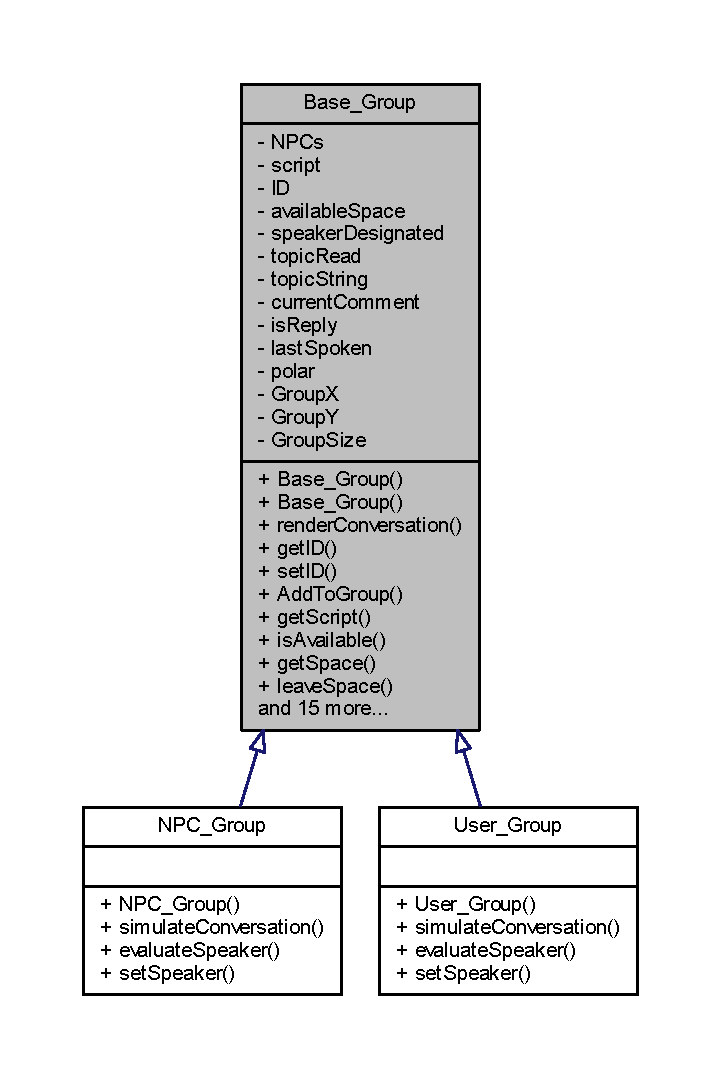
\includegraphics[width=346pt]{class_base___group__inherit__graph}
\end{center}
\end{figure}


Collaboration diagram for Base\+\_\+\+Group\+:\nopagebreak
\begin{figure}[H]
\begin{center}
\leavevmode
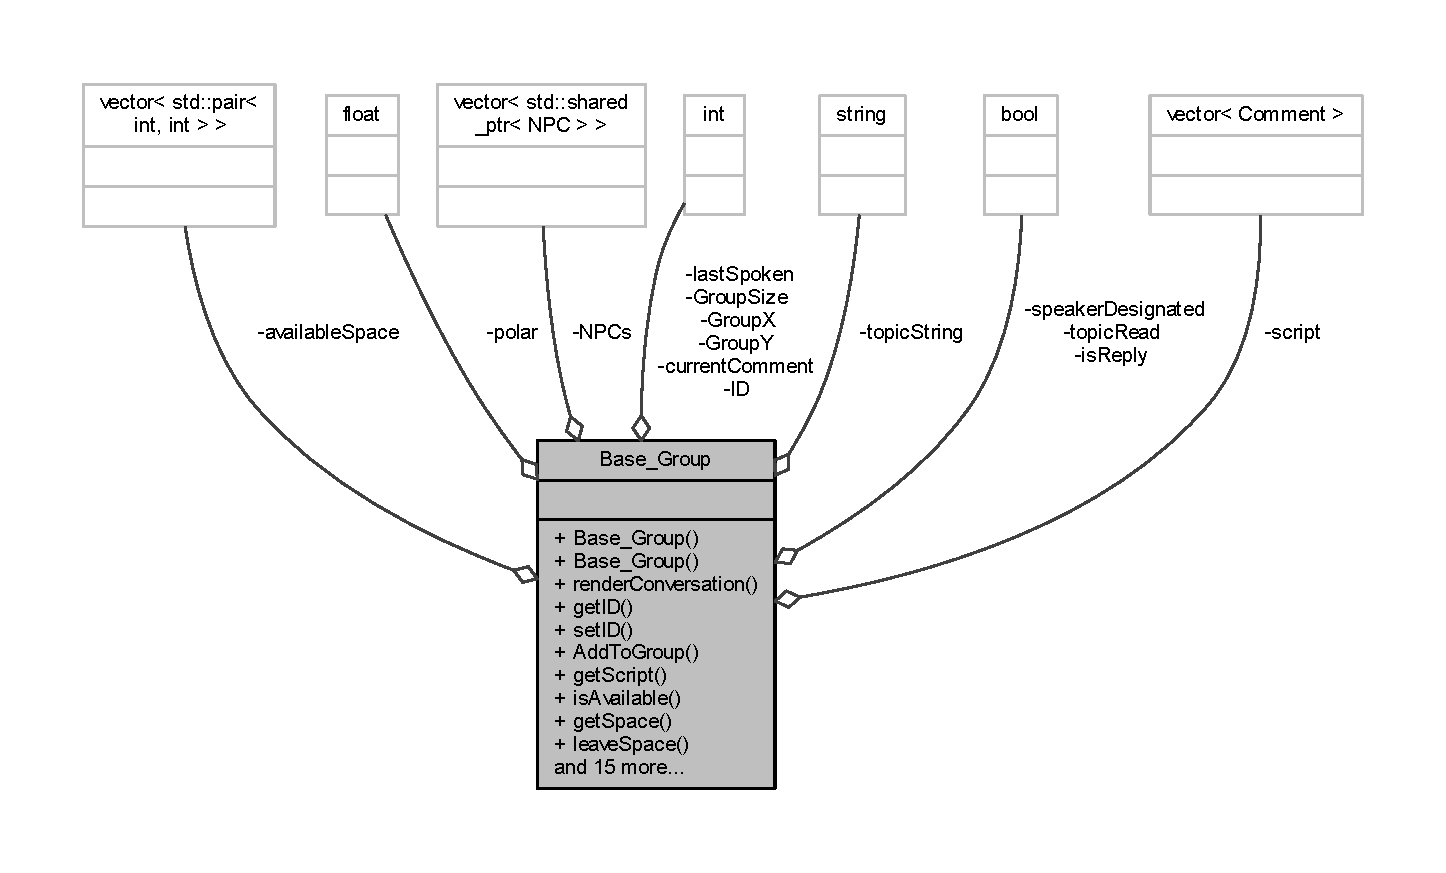
\includegraphics[width=350pt]{class_base___group__coll__graph}
\end{center}
\end{figure}
\subsection*{Public Member Functions}
\begin{DoxyCompactItemize}
\item 
\hyperlink{class_base___group_a96e70ee101d6430696f7b13b07190787}{Base\+\_\+\+Group} ()
\item 
\hyperlink{class_base___group_a056cdec4b61e453cd2125d5e0c5e3b57}{Base\+\_\+\+Group} (int x, int y, int size, std\+::string t\+Box\+File, std\+::string npc\+File, S\+D\+L\+\_\+\+Renderer $\ast$renderer, \hyperlink{class_topic}{Topic} tp)
\item 
void \hyperlink{class_base___group_a44b94b9d83c0aa526c9b51e2a46274cd}{render\+Conversation} (S\+D\+L\+\_\+\+Renderer $\ast$renderer)
\begin{DoxyCompactList}\small\item\em Renders the conversation to the S\+DL window. \end{DoxyCompactList}\item 
int \hyperlink{class_base___group_a7299ae154b26d741ac2f6f794bc3a544}{get\+ID} ()
\begin{DoxyCompactList}\small\item\em Retrieves the group ID. \end{DoxyCompactList}\item 
void \hyperlink{class_base___group_acc6c0adb1efeb47579da87d98450a98a}{set\+ID} (int id)
\begin{DoxyCompactList}\small\item\em Set the group ID. \end{DoxyCompactList}\item 
bool \hyperlink{class_base___group_a585d104ef8dfeaf0fdc0b2ef2089a4d1}{Add\+To\+Group} (std\+::shared\+\_\+ptr$<$ \hyperlink{class_n_p_c}{N\+PC} $>$ n\+N\+PC)
\begin{DoxyCompactList}\small\item\em Add an \hyperlink{class_n_p_c}{N\+PC} to the group. \end{DoxyCompactList}\item 
std\+::vector$<$ \hyperlink{class_comment}{Comment} $>$ \hyperlink{class_base___group_a48dadfbc8cdefca9bdd2c42b99115ad8}{get\+Script} ()
\begin{DoxyCompactList}\small\item\em Get the script of comments. \end{DoxyCompactList}\item 
bool \hyperlink{class_base___group_a6d806401632aa9f7795984bb2b4880f0}{is\+Available} ()
\begin{DoxyCompactList}\small\item\em Checks to if there is any avaialbe space in the groups. \end{DoxyCompactList}\item 
std\+::pair$<$ int, int $>$ \hyperlink{class_base___group_a4f6559c7a35e04e6355454df2e3be3b2}{get\+Space} ()
\begin{DoxyCompactList}\small\item\em Retrieves an open space from a group of \hyperlink{class_n_p_c}{N\+PC}\textquotesingle{}s. \end{DoxyCompactList}\item 
void \hyperlink{class_base___group_a0928f2c23abc827f6d387a5597324f6e}{leave\+Space} (std\+::shared\+\_\+ptr$<$ \hyperlink{class_n_p_c}{N\+PC} $>$ npc)
\begin{DoxyCompactList}\small\item\em Called when the \hyperlink{class_n_p_c}{N\+PC} wants to leave a group. \end{DoxyCompactList}\item 
bool \hyperlink{class_base___group_a76d7d9c0f35019dfaf7b2631eda863e1}{join\+Space} (std\+::shared\+\_\+ptr$<$ \hyperlink{class_n_p_c}{N\+PC} $>$ npc)
\begin{DoxyCompactList}\small\item\em Called when an \hyperlink{class_n_p_c}{N\+PC} wants to join a group. \end{DoxyCompactList}\item 
void \hyperlink{class_base___group_adebda6363b9f9097a8c866398e20f3c3}{clean\+Up\+Group} ()
\begin{DoxyCompactList}\small\item\em Clean up call, called when the group has nothing to talk about. \end{DoxyCompactList}\item 
int \hyperlink{class_base___group_a8fb88afb104365ec23447ee1f3649b4c}{get\+Last\+Spoken} ()
\begin{DoxyCompactList}\small\item\em Get the last \hyperlink{class_n_p_c}{N\+PC} who spoke in the conversation. \end{DoxyCompactList}\item 
void \hyperlink{class_base___group_a07e58c944f222f5c3d3b33c8adf83d14}{set\+Last\+Spoken} (int spoke)
\begin{DoxyCompactList}\small\item\em Set the last spoken \hyperlink{class_n_p_c}{N\+PC}. \end{DoxyCompactList}\item 
bool \hyperlink{class_base___group_a878700b51979d0acd3eb83cdfa4c0449}{get\+Is\+Reply} ()
\begin{DoxyCompactList}\small\item\em Check if the current comment is a reply. \end{DoxyCompactList}\item 
void \hyperlink{class_base___group_aebe2b457ac29aefcc7105908a61460c8}{set\+Is\+Reply} (bool reply)
\begin{DoxyCompactList}\small\item\em Set a bool to indicate the next comment is a reply. \end{DoxyCompactList}\item 
float \hyperlink{class_base___group_a57cd8ebf1eee11eab80816ee87223f36}{get\+Polar} ()
\begin{DoxyCompactList}\small\item\em Get the \hyperlink{class_n_p_c}{N\+PC}\textquotesingle{}s polarity score. \end{DoxyCompactList}\item 
void \hyperlink{class_base___group_a36ef627854f502a064fca8aea44a22fe}{set\+Polar} (float \hyperlink{class_base___group_a0c2dfa52ac107ec9564bfc42917e8ce0}{polar})
\begin{DoxyCompactList}\small\item\em Set the \hyperlink{class_n_p_c}{N\+PC}\textquotesingle{}s polarity score. \end{DoxyCompactList}\item 
void \hyperlink{class_base___group_a8c16feac44492aa68f4ee758662892c8}{update\+Script} ()
\begin{DoxyCompactList}\small\item\em Update the script. \end{DoxyCompactList}\item 
bool \hyperlink{class_base___group_a216c3f44a7ce30482ae933fc410d86a4}{in\+Group} (std\+::shared\+\_\+ptr$<$ \hyperlink{class_n_p_c}{N\+PC} $>$ npc)
\begin{DoxyCompactList}\small\item\em Returns a bool to indicate the parsed in \hyperlink{class_n_p_c}{N\+PC} belongs to the group. \end{DoxyCompactList}\item 
int \hyperlink{class_base___group_a3864a2806457151363344051f2814389}{Get\+Random\+Number} ()
\item 
virtual void \hyperlink{class_base___group_aa5080b6388c5974394bf326ce80bfa91}{simulate\+Conversation} (S\+D\+L\+\_\+\+Renderer $\ast$renderer, bool time, std\+::string boredom\+Level, T\+T\+F\+\_\+\+Font $\ast$font)
\begin{DoxyCompactList}\small\item\em Template methods to be inherited by child classes, these are the core classes for simulating conversation. \end{DoxyCompactList}\item 
virtual bool \hyperlink{class_base___group_a8264ff598ce7e789c6419e2e6eef08fd}{evaluate\+Speaker} ()
\item 
virtual void \hyperlink{class_base___group_ae35b3719076cf40d6577b4ae3779758c}{set\+Speaker} (std\+::string boredom\+Level)
\item 
std\+::vector$<$ std\+::shared\+\_\+ptr$<$ \hyperlink{class_n_p_c}{N\+PC} $>$ $>$ \hyperlink{class_base___group_a75eec9132aaf532b4429e0af76b31775}{get\+N\+P\+C\+List} ()
\begin{DoxyCompactList}\small\item\em Return the list of N\+P\+Cs. \end{DoxyCompactList}\end{DoxyCompactItemize}
\subsection*{Private Attributes}
\begin{DoxyCompactItemize}
\item 
std\+::vector$<$ std\+::shared\+\_\+ptr$<$ \hyperlink{class_n_p_c}{N\+PC} $>$ $>$ \hyperlink{class_base___group_a4757f3c06c73eea029f71b871c1d863e}{N\+P\+Cs}
\item 
std\+::vector$<$ \hyperlink{class_comment}{Comment} $>$ \hyperlink{class_base___group_a98fbcb0bb85a488e29db9465c18715cc}{script}
\item 
int \hyperlink{class_base___group_ae6ea7525642b45edafb56589d9945f90}{ID}
\item 
std\+::vector$<$ std\+::pair$<$ int, int $>$ $>$ \hyperlink{class_base___group_a8eb46d3107d53da0f5fbea2410b4b095}{available\+Space}
\item 
bool \hyperlink{class_base___group_ae6dfeabc8b679db58666e997653f4cec}{speaker\+Designated} = false
\item 
bool \hyperlink{class_base___group_a48710d3a08af8433d94756b4980ebe65}{topic\+Read} = true
\item 
std\+::string \hyperlink{class_base___group_a20e1ca90be1f271bf2256021d6325dfa}{topic\+String}
\item 
int \hyperlink{class_base___group_a9e1cd9c58ee0f2a67c3df992a553d625}{current\+Comment} = 0
\item 
bool \hyperlink{class_base___group_ad9dc72068ed8309820873de4084aa602}{is\+Reply}
\item 
int \hyperlink{class_base___group_aa031e7ea2c490eae2e8101fb4093da00}{last\+Spoken}
\item 
float \hyperlink{class_base___group_a0c2dfa52ac107ec9564bfc42917e8ce0}{polar}
\item 
int \hyperlink{class_base___group_a039388ca2feb6e676829839d9a3ff543}{GroupX}
\item 
int \hyperlink{class_base___group_adf6cb605c43eaa82f21150e84c629e17}{GroupY}
\item 
int \hyperlink{class_base___group_a44130e3b109f8fb9fb0142fda2a67b07}{Group\+Size}
\end{DoxyCompactItemize}


\subsection{Detailed Description}
The Base class for the \hyperlink{class_group}{Group} classes within the project 

Definition at line 14 of file Base\+\_\+\+Group.\+h.



\subsection{Constructor \& Destructor Documentation}
\mbox{\Hypertarget{class_base___group_a96e70ee101d6430696f7b13b07190787}\label{class_base___group_a96e70ee101d6430696f7b13b07190787}} 
\index{Base\+\_\+\+Group@{Base\+\_\+\+Group}!Base\+\_\+\+Group@{Base\+\_\+\+Group}}
\index{Base\+\_\+\+Group@{Base\+\_\+\+Group}!Base\+\_\+\+Group@{Base\+\_\+\+Group}}
\subsubsection{\texorpdfstring{Base\+\_\+\+Group()}{Base\_Group()}\hspace{0.1cm}{\footnotesize\ttfamily [1/2]}}
{\footnotesize\ttfamily Base\+\_\+\+Group\+::\+Base\+\_\+\+Group (\begin{DoxyParamCaption}{ }\end{DoxyParamCaption})}



Definition at line 11 of file Base\+\_\+\+Group.\+cpp.


\begin{DoxyCode}
12 \{
13 \}
\end{DoxyCode}
\mbox{\Hypertarget{class_base___group_a056cdec4b61e453cd2125d5e0c5e3b57}\label{class_base___group_a056cdec4b61e453cd2125d5e0c5e3b57}} 
\index{Base\+\_\+\+Group@{Base\+\_\+\+Group}!Base\+\_\+\+Group@{Base\+\_\+\+Group}}
\index{Base\+\_\+\+Group@{Base\+\_\+\+Group}!Base\+\_\+\+Group@{Base\+\_\+\+Group}}
\subsubsection{\texorpdfstring{Base\+\_\+\+Group()}{Base\_Group()}\hspace{0.1cm}{\footnotesize\ttfamily [2/2]}}
{\footnotesize\ttfamily Base\+\_\+\+Group\+::\+Base\+\_\+\+Group (\begin{DoxyParamCaption}\item[{int}]{x,  }\item[{int}]{y,  }\item[{int}]{size,  }\item[{std\+::string}]{t\+Box\+File,  }\item[{std\+::string}]{npc\+File,  }\item[{S\+D\+L\+\_\+\+Renderer $\ast$}]{renderer,  }\item[{\hyperlink{class_topic}{Topic}}]{tp }\end{DoxyParamCaption})}



Definition at line 16 of file Base\+\_\+\+Group.\+cpp.



References available\+Space, Topic\+::get\+Comments(), Topic\+::get\+Topic(), GroupX, GroupY, script, and topic\+String.


\begin{DoxyCode}
16                                                                                                            
                 : \hyperlink{class_base___group_a039388ca2feb6e676829839d9a3ff543}{GroupX}(x), \hyperlink{class_base___group_adf6cb605c43eaa82f21150e84c629e17}{GroupY}(y), \hyperlink{class_base___group_a44130e3b109f8fb9fb0142fda2a67b07}{GroupSize}(size)
17 \{
18     \hyperlink{class_base___group_a98fbcb0bb85a488e29db9465c18715cc}{script} = tp.\hyperlink{class_topic_ac800190b0f4f8ee514255cc75bce1f13}{getComments}();
19     \hyperlink{class_base___group_a20e1ca90be1f271bf2256021d6325dfa}{topicString} = tp.\hyperlink{class_topic_a9f6ad6642112c5f121a92aceb8df9c43}{getTopic}();
20     \hyperlink{class_base___group_a8eb46d3107d53da0f5fbea2410b4b095}{availableSpace}.push\_back(std::pair<int, int>(\hyperlink{class_base___group_a039388ca2feb6e676829839d9a3ff543}{GroupX}, 
      \hyperlink{class_base___group_adf6cb605c43eaa82f21150e84c629e17}{GroupY} - 35));
21     \hyperlink{class_base___group_a8eb46d3107d53da0f5fbea2410b4b095}{availableSpace}.push\_back(std::pair<int, int>(\hyperlink{class_base___group_a039388ca2feb6e676829839d9a3ff543}{GroupX} + 35, 
      \hyperlink{class_base___group_adf6cb605c43eaa82f21150e84c629e17}{GroupY} - 17));
22     \hyperlink{class_base___group_a8eb46d3107d53da0f5fbea2410b4b095}{availableSpace}.push\_back(std::pair<int, int>(\hyperlink{class_base___group_a039388ca2feb6e676829839d9a3ff543}{GroupX} + 35, 
      \hyperlink{class_base___group_adf6cb605c43eaa82f21150e84c629e17}{GroupY} + 17));
23     \hyperlink{class_base___group_a8eb46d3107d53da0f5fbea2410b4b095}{availableSpace}.push\_back(std::pair<int, int>(\hyperlink{class_base___group_a039388ca2feb6e676829839d9a3ff543}{GroupX}, 
      \hyperlink{class_base___group_adf6cb605c43eaa82f21150e84c629e17}{GroupY} + 35));
24     \hyperlink{class_base___group_a8eb46d3107d53da0f5fbea2410b4b095}{availableSpace}.push\_back(std::pair<int, int>(\hyperlink{class_base___group_a039388ca2feb6e676829839d9a3ff543}{GroupX} - 35, 
      \hyperlink{class_base___group_adf6cb605c43eaa82f21150e84c629e17}{GroupY} + 17));
25     \hyperlink{class_base___group_a8eb46d3107d53da0f5fbea2410b4b095}{availableSpace}.push\_back(std::pair<int, int>(\hyperlink{class_base___group_a039388ca2feb6e676829839d9a3ff543}{GroupX} - 35, 
      \hyperlink{class_base___group_adf6cb605c43eaa82f21150e84c629e17}{GroupY} - 17));
26 \}
\end{DoxyCode}


\subsection{Member Function Documentation}
\mbox{\Hypertarget{class_base___group_a585d104ef8dfeaf0fdc0b2ef2089a4d1}\label{class_base___group_a585d104ef8dfeaf0fdc0b2ef2089a4d1}} 
\index{Base\+\_\+\+Group@{Base\+\_\+\+Group}!Add\+To\+Group@{Add\+To\+Group}}
\index{Add\+To\+Group@{Add\+To\+Group}!Base\+\_\+\+Group@{Base\+\_\+\+Group}}
\subsubsection{\texorpdfstring{Add\+To\+Group()}{AddToGroup()}}
{\footnotesize\ttfamily bool Base\+\_\+\+Group\+::\+Add\+To\+Group (\begin{DoxyParamCaption}\item[{std\+::shared\+\_\+ptr$<$ \hyperlink{class_n_p_c}{N\+PC} $>$}]{n\+N\+PC }\end{DoxyParamCaption})}



Add an \hyperlink{class_n_p_c}{N\+PC} to the group. 



Definition at line 95 of file Base\+\_\+\+Group.\+cpp.



References available\+Space, get\+Space(), is\+Available(), and N\+P\+Cs.


\begin{DoxyCode}
96 \{
97     \textcolor{keywordtype}{bool} success = \textcolor{keyword}{false};
98     \textcolor{keywordflow}{if} (\hyperlink{class_base___group_a4757f3c06c73eea029f71b871c1d863e}{NPCs}.size() < 6)
99     \{
100         \textcolor{keywordflow}{if} (\hyperlink{class_base___group_a6d806401632aa9f7795984bb2b4880f0}{isAvailable}())
101         \{
102             std::pair<int, int> newPos = \hyperlink{class_base___group_a4f6559c7a35e04e6355454df2e3be3b2}{getSpace}();
103             nNPC->setEndGoal(newPos);
104             nNPC->setX(newPos.first);
105             nNPC->setY(newPos.second);
106             \hyperlink{class_base___group_a8eb46d3107d53da0f5fbea2410b4b095}{availableSpace}.erase(std::remove(\hyperlink{class_base___group_a8eb46d3107d53da0f5fbea2410b4b095}{availableSpace}.begin(), 
      \hyperlink{class_base___group_a8eb46d3107d53da0f5fbea2410b4b095}{availableSpace}.end(), \hyperlink{class_base___group_a8eb46d3107d53da0f5fbea2410b4b095}{availableSpace}[0]), 
      \hyperlink{class_base___group_a8eb46d3107d53da0f5fbea2410b4b095}{availableSpace}.end());
107             \textcolor{keywordflow}{if} (\hyperlink{class_base___group_a4757f3c06c73eea029f71b871c1d863e}{NPCs}.size() == 0)
108             \{
109                 nNPC->setSpeaking(\textcolor{keyword}{true});
110             \}
111             \hyperlink{class_base___group_a4757f3c06c73eea029f71b871c1d863e}{NPCs}.push\_back(nNPC);
112             success = \textcolor{keyword}{true};
113         \}
114         \textcolor{keywordflow}{else}
115             \textcolor{keywordflow}{return} success;
116     \}
117     \textcolor{keywordflow}{else}
118     \{
119         \textcolor{keywordflow}{return} success;
120     \}
121 
122     \textcolor{keywordflow}{return} success;
123 \}
\end{DoxyCode}
\mbox{\Hypertarget{class_base___group_adebda6363b9f9097a8c866398e20f3c3}\label{class_base___group_adebda6363b9f9097a8c866398e20f3c3}} 
\index{Base\+\_\+\+Group@{Base\+\_\+\+Group}!clean\+Up\+Group@{clean\+Up\+Group}}
\index{clean\+Up\+Group@{clean\+Up\+Group}!Base\+\_\+\+Group@{Base\+\_\+\+Group}}
\subsubsection{\texorpdfstring{clean\+Up\+Group()}{cleanUpGroup()}}
{\footnotesize\ttfamily void Base\+\_\+\+Group\+::clean\+Up\+Group (\begin{DoxyParamCaption}{ }\end{DoxyParamCaption})}



Clean up call, called when the group has nothing to talk about. 



Definition at line 224 of file Base\+\_\+\+Group.\+cpp.



References leave\+Space(), and N\+P\+Cs.


\begin{DoxyCode}
225 \{
226     \textcolor{keywordflow}{for} (\textcolor{keywordtype}{int} i = 0; i < \hyperlink{class_base___group_a4757f3c06c73eea029f71b871c1d863e}{NPCs}.size(); i++)
227     \{
228         \hyperlink{class_base___group_a4757f3c06c73eea029f71b871c1d863e}{NPCs}[i]->setIdle(\textcolor{keyword}{true});
229         \hyperlink{class_base___group_a4757f3c06c73eea029f71b871c1d863e}{NPCs}[i]->setSpeaking(\textcolor{keyword}{false});
230         \hyperlink{class_base___group_a4757f3c06c73eea029f71b871c1d863e}{NPCs}[i]->setReading(\textcolor{keyword}{false});
231         \hyperlink{class_base___group_a4757f3c06c73eea029f71b871c1d863e}{NPCs}[i]->setText(\textcolor{stringliteral}{""});
232         \hyperlink{class_base___group_a4757f3c06c73eea029f71b871c1d863e}{NPCs}[i]->setGroupID(-1);
233         \hyperlink{class_base___group_a0928f2c23abc827f6d387a5597324f6e}{leaveSpace}(\hyperlink{class_base___group_a4757f3c06c73eea029f71b871c1d863e}{NPCs}[i]);
234     \}
235 \}
\end{DoxyCode}
\mbox{\Hypertarget{class_base___group_a8264ff598ce7e789c6419e2e6eef08fd}\label{class_base___group_a8264ff598ce7e789c6419e2e6eef08fd}} 
\index{Base\+\_\+\+Group@{Base\+\_\+\+Group}!evaluate\+Speaker@{evaluate\+Speaker}}
\index{evaluate\+Speaker@{evaluate\+Speaker}!Base\+\_\+\+Group@{Base\+\_\+\+Group}}
\subsubsection{\texorpdfstring{evaluate\+Speaker()}{evaluateSpeaker()}}
{\footnotesize\ttfamily bool Base\+\_\+\+Group\+::evaluate\+Speaker (\begin{DoxyParamCaption}{ }\end{DoxyParamCaption})\hspace{0.3cm}{\ttfamily [virtual]}}



Reimplemented in \hyperlink{class_n_p_c___group_a2e0b8772b42985bd7e87359013918601}{N\+P\+C\+\_\+\+Group}, and \hyperlink{class_user___group_a40051b822a0f0dd126b95d0f0fd28eff}{User\+\_\+\+Group}.



Definition at line 254 of file Base\+\_\+\+Group.\+cpp.


\begin{DoxyCode}
255 \{
256     \textcolor{keywordflow}{return} \textcolor{keyword}{false};
257 \}
\end{DoxyCode}
\mbox{\Hypertarget{class_base___group_a7299ae154b26d741ac2f6f794bc3a544}\label{class_base___group_a7299ae154b26d741ac2f6f794bc3a544}} 
\index{Base\+\_\+\+Group@{Base\+\_\+\+Group}!get\+ID@{get\+ID}}
\index{get\+ID@{get\+ID}!Base\+\_\+\+Group@{Base\+\_\+\+Group}}
\subsubsection{\texorpdfstring{get\+I\+D()}{getID()}}
{\footnotesize\ttfamily int Base\+\_\+\+Group\+::get\+ID (\begin{DoxyParamCaption}{ }\end{DoxyParamCaption})}



Retrieves the group ID. 



Definition at line 73 of file Base\+\_\+\+Group.\+cpp.



References ID.



Referenced by leave\+Space(), User\+\_\+\+Group\+::set\+Speaker(), and N\+P\+C\+\_\+\+Group\+::set\+Speaker().


\begin{DoxyCode}
74 \{
75     \textcolor{keywordflow}{return} \hyperlink{class_base___group_ae6ea7525642b45edafb56589d9945f90}{ID};
76 \}
\end{DoxyCode}
\mbox{\Hypertarget{class_base___group_a878700b51979d0acd3eb83cdfa4c0449}\label{class_base___group_a878700b51979d0acd3eb83cdfa4c0449}} 
\index{Base\+\_\+\+Group@{Base\+\_\+\+Group}!get\+Is\+Reply@{get\+Is\+Reply}}
\index{get\+Is\+Reply@{get\+Is\+Reply}!Base\+\_\+\+Group@{Base\+\_\+\+Group}}
\subsubsection{\texorpdfstring{get\+Is\+Reply()}{getIsReply()}}
{\footnotesize\ttfamily bool Base\+\_\+\+Group\+::get\+Is\+Reply (\begin{DoxyParamCaption}{ }\end{DoxyParamCaption})}



Check if the current comment is a reply. 



Definition at line 148 of file Base\+\_\+\+Group.\+cpp.



References is\+Reply.



Referenced by N\+P\+C\+\_\+\+Group\+::simulate\+Conversation().


\begin{DoxyCode}
149 \{
150     \textcolor{keywordflow}{return} \hyperlink{class_base___group_ad9dc72068ed8309820873de4084aa602}{isReply};
151 \}
\end{DoxyCode}
\mbox{\Hypertarget{class_base___group_a8fb88afb104365ec23447ee1f3649b4c}\label{class_base___group_a8fb88afb104365ec23447ee1f3649b4c}} 
\index{Base\+\_\+\+Group@{Base\+\_\+\+Group}!get\+Last\+Spoken@{get\+Last\+Spoken}}
\index{get\+Last\+Spoken@{get\+Last\+Spoken}!Base\+\_\+\+Group@{Base\+\_\+\+Group}}
\subsubsection{\texorpdfstring{get\+Last\+Spoken()}{getLastSpoken()}}
{\footnotesize\ttfamily int Base\+\_\+\+Group\+::get\+Last\+Spoken (\begin{DoxyParamCaption}{ }\end{DoxyParamCaption})}



Get the last \hyperlink{class_n_p_c}{N\+PC} who spoke in the conversation. 



Definition at line 138 of file Base\+\_\+\+Group.\+cpp.



References last\+Spoken.



Referenced by N\+P\+C\+\_\+\+Group\+::simulate\+Conversation().


\begin{DoxyCode}
139 \{
140     \textcolor{keywordflow}{return} \hyperlink{class_base___group_aa031e7ea2c490eae2e8101fb4093da00}{lastSpoken};
141 \}
\end{DoxyCode}
\mbox{\Hypertarget{class_base___group_a75eec9132aaf532b4429e0af76b31775}\label{class_base___group_a75eec9132aaf532b4429e0af76b31775}} 
\index{Base\+\_\+\+Group@{Base\+\_\+\+Group}!get\+N\+P\+C\+List@{get\+N\+P\+C\+List}}
\index{get\+N\+P\+C\+List@{get\+N\+P\+C\+List}!Base\+\_\+\+Group@{Base\+\_\+\+Group}}
\subsubsection{\texorpdfstring{get\+N\+P\+C\+List()}{getNPCList()}}
{\footnotesize\ttfamily std\+::vector$<$ std\+::shared\+\_\+ptr$<$ \hyperlink{class_n_p_c}{N\+PC} $>$ $>$ Base\+\_\+\+Group\+::get\+N\+P\+C\+List (\begin{DoxyParamCaption}{ }\end{DoxyParamCaption})}



Return the list of N\+P\+Cs. 



Definition at line 133 of file Base\+\_\+\+Group.\+cpp.



References N\+P\+Cs.



Referenced by User\+\_\+\+Group\+::evaluate\+Speaker(), N\+P\+C\+\_\+\+Group\+::evaluate\+Speaker(), User\+\_\+\+Group\+::set\+Speaker(), N\+P\+C\+\_\+\+Group\+::set\+Speaker(), and N\+P\+C\+\_\+\+Group\+::simulate\+Conversation().


\begin{DoxyCode}
134 \{
135     \textcolor{keywordflow}{return} \hyperlink{class_base___group_a4757f3c06c73eea029f71b871c1d863e}{NPCs};
136 \}
\end{DoxyCode}
\mbox{\Hypertarget{class_base___group_a57cd8ebf1eee11eab80816ee87223f36}\label{class_base___group_a57cd8ebf1eee11eab80816ee87223f36}} 
\index{Base\+\_\+\+Group@{Base\+\_\+\+Group}!get\+Polar@{get\+Polar}}
\index{get\+Polar@{get\+Polar}!Base\+\_\+\+Group@{Base\+\_\+\+Group}}
\subsubsection{\texorpdfstring{get\+Polar()}{getPolar()}}
{\footnotesize\ttfamily float Base\+\_\+\+Group\+::get\+Polar (\begin{DoxyParamCaption}{ }\end{DoxyParamCaption})}



Get the \hyperlink{class_n_p_c}{N\+PC}\textquotesingle{}s polarity score. 



Definition at line 158 of file Base\+\_\+\+Group.\+cpp.



References polar.



Referenced by N\+P\+C\+\_\+\+Group\+::simulate\+Conversation().


\begin{DoxyCode}
159 \{
160     \textcolor{keywordflow}{return} \hyperlink{class_base___group_a0c2dfa52ac107ec9564bfc42917e8ce0}{polar};
161 \}
\end{DoxyCode}
\mbox{\Hypertarget{class_base___group_a3864a2806457151363344051f2814389}\label{class_base___group_a3864a2806457151363344051f2814389}} 
\index{Base\+\_\+\+Group@{Base\+\_\+\+Group}!Get\+Random\+Number@{Get\+Random\+Number}}
\index{Get\+Random\+Number@{Get\+Random\+Number}!Base\+\_\+\+Group@{Base\+\_\+\+Group}}
\subsubsection{\texorpdfstring{Get\+Random\+Number()}{GetRandomNumber()}}
{\footnotesize\ttfamily int Base\+\_\+\+Group\+::\+Get\+Random\+Number (\begin{DoxyParamCaption}{ }\end{DoxyParamCaption})}



Definition at line 171 of file Base\+\_\+\+Group.\+cpp.



References last\+Spoken, and N\+P\+Cs.



Referenced by User\+\_\+\+Group\+::set\+Speaker(), and N\+P\+C\+\_\+\+Group\+::set\+Speaker().


\begin{DoxyCode}
172 \{
173     \textcolor{keywordflow}{if} (\hyperlink{class_base___group_a4757f3c06c73eea029f71b871c1d863e}{NPCs}.size() > 0)
174     \{
175         \textcolor{keywordtype}{int} gSize = \hyperlink{class_base___group_a4757f3c06c73eea029f71b871c1d863e}{NPCs}.size();
176 
177         std::mt19937 rng;
178         rng.seed(std::random\_device()());
179         std::uniform\_int\_distribution<std::mt19937::result\_type> distGroup(0, gSize - 1);
180 
181         \textcolor{keywordtype}{int} random = distGroup(rng);
182         \textcolor{comment}{//if the random number matches our current NPC, change its value}
183         \textcolor{keywordflow}{if} (random == \hyperlink{class_base___group_aa031e7ea2c490eae2e8101fb4093da00}{lastSpoken})
184         \{
185             \textcolor{keywordflow}{if} (random == \hyperlink{class_base___group_a4757f3c06c73eea029f71b871c1d863e}{NPCs}.size() - 1)
186                 random--;
187             \textcolor{keywordflow}{else}
188                 random++;
189         \}
190 
191         \textcolor{keywordflow}{if} (random < 0)
192             random = \hyperlink{class_base___group_a4757f3c06c73eea029f71b871c1d863e}{NPCs}.size() - 1;
193 
194         \textcolor{keywordflow}{if} (\hyperlink{class_base___group_a4757f3c06c73eea029f71b871c1d863e}{NPCs}[random]->getIdle() == \textcolor{keyword}{true})
195         \{
196             random--;
197             \textcolor{keywordflow}{if} (random == \hyperlink{class_base___group_aa031e7ea2c490eae2e8101fb4093da00}{lastSpoken})
198                 random + 2;
199         \}
200 
201         \textcolor{keywordflow}{if} (random < 0)
202             random = \hyperlink{class_base___group_a4757f3c06c73eea029f71b871c1d863e}{NPCs}.size() - 1;
203 
204         \textcolor{keywordflow}{return} random;
205     \}
206     \textcolor{keywordflow}{return} 0;
207 \}
\end{DoxyCode}
\mbox{\Hypertarget{class_base___group_a48dadfbc8cdefca9bdd2c42b99115ad8}\label{class_base___group_a48dadfbc8cdefca9bdd2c42b99115ad8}} 
\index{Base\+\_\+\+Group@{Base\+\_\+\+Group}!get\+Script@{get\+Script}}
\index{get\+Script@{get\+Script}!Base\+\_\+\+Group@{Base\+\_\+\+Group}}
\subsubsection{\texorpdfstring{get\+Script()}{getScript()}}
{\footnotesize\ttfamily std\+::vector$<$ \hyperlink{class_comment}{Comment} $>$ Base\+\_\+\+Group\+::get\+Script (\begin{DoxyParamCaption}{ }\end{DoxyParamCaption})}



Get the script of comments. 



Definition at line 125 of file Base\+\_\+\+Group.\+cpp.



References script.



Referenced by User\+\_\+\+Group\+::set\+Speaker(), and N\+P\+C\+\_\+\+Group\+::simulate\+Conversation().


\begin{DoxyCode}
126 \{
127     \textcolor{keywordflow}{return} \hyperlink{class_base___group_a98fbcb0bb85a488e29db9465c18715cc}{script};
128 \}
\end{DoxyCode}
\mbox{\Hypertarget{class_base___group_a4f6559c7a35e04e6355454df2e3be3b2}\label{class_base___group_a4f6559c7a35e04e6355454df2e3be3b2}} 
\index{Base\+\_\+\+Group@{Base\+\_\+\+Group}!get\+Space@{get\+Space}}
\index{get\+Space@{get\+Space}!Base\+\_\+\+Group@{Base\+\_\+\+Group}}
\subsubsection{\texorpdfstring{get\+Space()}{getSpace()}}
{\footnotesize\ttfamily std\+::pair$<$ int, int $>$ Base\+\_\+\+Group\+::get\+Space (\begin{DoxyParamCaption}{ }\end{DoxyParamCaption})}



Retrieves an open space from a group of \hyperlink{class_n_p_c}{N\+PC}\textquotesingle{}s. 



Definition at line 36 of file Base\+\_\+\+Group.\+cpp.



References available\+Space, and is\+Available().



Referenced by Add\+To\+Group(), and join\+Space().


\begin{DoxyCode}
37 \{
38     \textcolor{keywordflow}{if} (\hyperlink{class_base___group_a6d806401632aa9f7795984bb2b4880f0}{isAvailable}()) \{
39         std::pair<int, int> recoveredSpace = \hyperlink{class_base___group_a8eb46d3107d53da0f5fbea2410b4b095}{availableSpace}[0];
40         \textcolor{keywordflow}{return} recoveredSpace;
41     \}
42 \}
\end{DoxyCode}
\mbox{\Hypertarget{class_base___group_a216c3f44a7ce30482ae933fc410d86a4}\label{class_base___group_a216c3f44a7ce30482ae933fc410d86a4}} 
\index{Base\+\_\+\+Group@{Base\+\_\+\+Group}!in\+Group@{in\+Group}}
\index{in\+Group@{in\+Group}!Base\+\_\+\+Group@{Base\+\_\+\+Group}}
\subsubsection{\texorpdfstring{in\+Group()}{inGroup()}}
{\footnotesize\ttfamily bool Base\+\_\+\+Group\+::in\+Group (\begin{DoxyParamCaption}\item[{std\+::shared\+\_\+ptr$<$ \hyperlink{class_n_p_c}{N\+PC} $>$}]{npc }\end{DoxyParamCaption})}



Returns a bool to indicate the parsed in \hyperlink{class_n_p_c}{N\+PC} belongs to the group. 



Definition at line 237 of file Base\+\_\+\+Group.\+cpp.



References N\+P\+Cs.


\begin{DoxyCode}
238 \{
239     \textcolor{keywordflow}{for} (\textcolor{keywordtype}{int} i = 0; i < \hyperlink{class_base___group_a4757f3c06c73eea029f71b871c1d863e}{NPCs}.size(); i++)
240     \{
241         \textcolor{keywordflow}{if} (\hyperlink{class_base___group_a4757f3c06c73eea029f71b871c1d863e}{NPCs}[i] == npc)
242             \textcolor{keywordflow}{return} \textcolor{keyword}{true};
243     \}
244     \textcolor{keywordflow}{return} \textcolor{keyword}{false};
245 \}
\end{DoxyCode}
\mbox{\Hypertarget{class_base___group_a6d806401632aa9f7795984bb2b4880f0}\label{class_base___group_a6d806401632aa9f7795984bb2b4880f0}} 
\index{Base\+\_\+\+Group@{Base\+\_\+\+Group}!is\+Available@{is\+Available}}
\index{is\+Available@{is\+Available}!Base\+\_\+\+Group@{Base\+\_\+\+Group}}
\subsubsection{\texorpdfstring{is\+Available()}{isAvailable()}}
{\footnotesize\ttfamily bool Base\+\_\+\+Group\+::is\+Available (\begin{DoxyParamCaption}{ }\end{DoxyParamCaption})}



Checks to if there is any avaialbe space in the groups. 



Definition at line 28 of file Base\+\_\+\+Group.\+cpp.



References available\+Space.



Referenced by Add\+To\+Group(), get\+Space(), and join\+Space().


\begin{DoxyCode}
29 \{
30     \textcolor{keywordflow}{if} (\hyperlink{class_base___group_a8eb46d3107d53da0f5fbea2410b4b095}{availableSpace}.size() > 0)
31         \textcolor{keywordflow}{return} \textcolor{keyword}{true};
32     \textcolor{keywordflow}{else}
33         \textcolor{keywordflow}{return} \textcolor{keyword}{false};
34 \}
\end{DoxyCode}
\mbox{\Hypertarget{class_base___group_a76d7d9c0f35019dfaf7b2631eda863e1}\label{class_base___group_a76d7d9c0f35019dfaf7b2631eda863e1}} 
\index{Base\+\_\+\+Group@{Base\+\_\+\+Group}!join\+Space@{join\+Space}}
\index{join\+Space@{join\+Space}!Base\+\_\+\+Group@{Base\+\_\+\+Group}}
\subsubsection{\texorpdfstring{join\+Space()}{joinSpace()}}
{\footnotesize\ttfamily bool Base\+\_\+\+Group\+::join\+Space (\begin{DoxyParamCaption}\item[{std\+::shared\+\_\+ptr$<$ \hyperlink{class_n_p_c}{N\+PC} $>$}]{npc }\end{DoxyParamCaption})}



Called when an \hyperlink{class_n_p_c}{N\+PC} wants to join a group. 



Definition at line 44 of file Base\+\_\+\+Group.\+cpp.



References available\+Space, get\+Space(), ID, is\+Available(), and N\+P\+Cs.


\begin{DoxyCode}
45 \{
46     \textcolor{keywordtype}{bool} success = \textcolor{keyword}{false};
47     \textcolor{keywordflow}{if} (\hyperlink{class_base___group_a4757f3c06c73eea029f71b871c1d863e}{NPCs}.size() < 6)
48     \{
49         \textcolor{keywordflow}{if} (\hyperlink{class_base___group_a6d806401632aa9f7795984bb2b4880f0}{isAvailable}())
50         \{
51             std::pair<int, int> newPos = \hyperlink{class_base___group_a4f6559c7a35e04e6355454df2e3be3b2}{getSpace}();
52             \hyperlink{class_base___group_a8eb46d3107d53da0f5fbea2410b4b095}{availableSpace}.erase(std::remove(\hyperlink{class_base___group_a8eb46d3107d53da0f5fbea2410b4b095}{availableSpace}.begin(), 
      \hyperlink{class_base___group_a8eb46d3107d53da0f5fbea2410b4b095}{availableSpace}.end(), \hyperlink{class_base___group_a8eb46d3107d53da0f5fbea2410b4b095}{availableSpace}[0]), 
      \hyperlink{class_base___group_a8eb46d3107d53da0f5fbea2410b4b095}{availableSpace}.end());
53             npc->setEndGoal(newPos);
54             \textcolor{keywordflow}{if} (\hyperlink{class_base___group_a4757f3c06c73eea029f71b871c1d863e}{NPCs}.size() == 0)
55             \{
56                 npc->setSpeaking(\textcolor{keyword}{true});
57             \}
58             npc->setGroupID(\hyperlink{class_base___group_ae6ea7525642b45edafb56589d9945f90}{ID});
59             \hyperlink{class_base___group_a4757f3c06c73eea029f71b871c1d863e}{NPCs}.push\_back(npc);
60             success = \textcolor{keyword}{true};
61         \}
62         \textcolor{keywordflow}{else}
63             \textcolor{keywordflow}{return} success;
64     \}
65     \textcolor{keywordflow}{else}
66     \{
67         \textcolor{keywordflow}{return} success;
68     \}
69 
70     \textcolor{keywordflow}{return} success;
71 \}
\end{DoxyCode}
\mbox{\Hypertarget{class_base___group_a0928f2c23abc827f6d387a5597324f6e}\label{class_base___group_a0928f2c23abc827f6d387a5597324f6e}} 
\index{Base\+\_\+\+Group@{Base\+\_\+\+Group}!leave\+Space@{leave\+Space}}
\index{leave\+Space@{leave\+Space}!Base\+\_\+\+Group@{Base\+\_\+\+Group}}
\subsubsection{\texorpdfstring{leave\+Space()}{leaveSpace()}}
{\footnotesize\ttfamily void Base\+\_\+\+Group\+::leave\+Space (\begin{DoxyParamCaption}\item[{std\+::shared\+\_\+ptr$<$ \hyperlink{class_n_p_c}{N\+PC} $>$}]{npc }\end{DoxyParamCaption})}



Called when the \hyperlink{class_n_p_c}{N\+PC} wants to leave a group. 



Definition at line 83 of file Base\+\_\+\+Group.\+cpp.



References available\+Space, get\+I\+D(), and N\+P\+Cs.



Referenced by clean\+Up\+Group().


\begin{DoxyCode}
84 \{
85     \textcolor{keywordflow}{for} (\textcolor{keywordtype}{int} i = 0; i < \hyperlink{class_base___group_a4757f3c06c73eea029f71b871c1d863e}{NPCs}.size(); i++)
86     \{
87         \textcolor{keywordflow}{if} (\hyperlink{class_base___group_a4757f3c06c73eea029f71b871c1d863e}{NPCs}[i]->\hyperlink{class_base___group_a7299ae154b26d741ac2f6f794bc3a544}{getID}() == npc->getID())
88         \{
89             \hyperlink{class_base___group_a8eb46d3107d53da0f5fbea2410b4b095}{availableSpace}.push\_back(std::pair<int, int>(npc->getX(), npc->getY()));
90             \hyperlink{class_base___group_a4757f3c06c73eea029f71b871c1d863e}{NPCs}.erase(std::remove(\hyperlink{class_base___group_a4757f3c06c73eea029f71b871c1d863e}{NPCs}.begin(), \hyperlink{class_base___group_a4757f3c06c73eea029f71b871c1d863e}{NPCs}.end(), npc), 
      \hyperlink{class_base___group_a4757f3c06c73eea029f71b871c1d863e}{NPCs}.end());
91         \}
92     \}
93 \}
\end{DoxyCode}
\mbox{\Hypertarget{class_base___group_a44b94b9d83c0aa526c9b51e2a46274cd}\label{class_base___group_a44b94b9d83c0aa526c9b51e2a46274cd}} 
\index{Base\+\_\+\+Group@{Base\+\_\+\+Group}!render\+Conversation@{render\+Conversation}}
\index{render\+Conversation@{render\+Conversation}!Base\+\_\+\+Group@{Base\+\_\+\+Group}}
\subsubsection{\texorpdfstring{render\+Conversation()}{renderConversation()}}
{\footnotesize\ttfamily void Base\+\_\+\+Group\+::render\+Conversation (\begin{DoxyParamCaption}\item[{S\+D\+L\+\_\+\+Renderer $\ast$}]{renderer }\end{DoxyParamCaption})}



Renders the conversation to the S\+DL window. 



Definition at line 211 of file Base\+\_\+\+Group.\+cpp.



References N\+P\+Cs.


\begin{DoxyCode}
212 \{
213     std::vector<std::shared\_ptr<NPC>>::iterator npcIterator;
214     \textcolor{keywordflow}{for} (npcIterator = \hyperlink{class_base___group_a4757f3c06c73eea029f71b871c1d863e}{NPCs}.begin(); npcIterator != \hyperlink{class_base___group_a4757f3c06c73eea029f71b871c1d863e}{NPCs}.end(); npcIterator++)
215     \{
216         \textcolor{comment}{//render the comment of the NPC currently speaking}
217         \textcolor{keywordflow}{if} ((*npcIterator)->getSpeaking()) \{
218             (*npcIterator)->renderBox(renderer);
219             (*npcIterator)->renderComment(renderer);
220         \}
221     \}
222 \}
\end{DoxyCode}
\mbox{\Hypertarget{class_base___group_acc6c0adb1efeb47579da87d98450a98a}\label{class_base___group_acc6c0adb1efeb47579da87d98450a98a}} 
\index{Base\+\_\+\+Group@{Base\+\_\+\+Group}!set\+ID@{set\+ID}}
\index{set\+ID@{set\+ID}!Base\+\_\+\+Group@{Base\+\_\+\+Group}}
\subsubsection{\texorpdfstring{set\+I\+D()}{setID()}}
{\footnotesize\ttfamily void Base\+\_\+\+Group\+::set\+ID (\begin{DoxyParamCaption}\item[{int}]{id }\end{DoxyParamCaption})}



Set the group ID. 



Definition at line 78 of file Base\+\_\+\+Group.\+cpp.



References ID.


\begin{DoxyCode}
79 \{
80     \hyperlink{class_base___group_ae6ea7525642b45edafb56589d9945f90}{ID} = id;
81 \}
\end{DoxyCode}
\mbox{\Hypertarget{class_base___group_aebe2b457ac29aefcc7105908a61460c8}\label{class_base___group_aebe2b457ac29aefcc7105908a61460c8}} 
\index{Base\+\_\+\+Group@{Base\+\_\+\+Group}!set\+Is\+Reply@{set\+Is\+Reply}}
\index{set\+Is\+Reply@{set\+Is\+Reply}!Base\+\_\+\+Group@{Base\+\_\+\+Group}}
\subsubsection{\texorpdfstring{set\+Is\+Reply()}{setIsReply()}}
{\footnotesize\ttfamily void Base\+\_\+\+Group\+::set\+Is\+Reply (\begin{DoxyParamCaption}\item[{bool}]{reply }\end{DoxyParamCaption})}



Set a bool to indicate the next comment is a reply. 



Definition at line 153 of file Base\+\_\+\+Group.\+cpp.



References is\+Reply.



Referenced by N\+P\+C\+\_\+\+Group\+::simulate\+Conversation().


\begin{DoxyCode}
154 \{
155     \hyperlink{class_base___group_ad9dc72068ed8309820873de4084aa602}{isReply} = reply;
156 \}
\end{DoxyCode}
\mbox{\Hypertarget{class_base___group_a07e58c944f222f5c3d3b33c8adf83d14}\label{class_base___group_a07e58c944f222f5c3d3b33c8adf83d14}} 
\index{Base\+\_\+\+Group@{Base\+\_\+\+Group}!set\+Last\+Spoken@{set\+Last\+Spoken}}
\index{set\+Last\+Spoken@{set\+Last\+Spoken}!Base\+\_\+\+Group@{Base\+\_\+\+Group}}
\subsubsection{\texorpdfstring{set\+Last\+Spoken()}{setLastSpoken()}}
{\footnotesize\ttfamily void Base\+\_\+\+Group\+::set\+Last\+Spoken (\begin{DoxyParamCaption}\item[{int}]{spoke }\end{DoxyParamCaption})}



Set the last spoken \hyperlink{class_n_p_c}{N\+PC}. 



Definition at line 143 of file Base\+\_\+\+Group.\+cpp.



References last\+Spoken.



Referenced by N\+P\+C\+\_\+\+Group\+::simulate\+Conversation().


\begin{DoxyCode}
144 \{
145     \hyperlink{class_base___group_aa031e7ea2c490eae2e8101fb4093da00}{lastSpoken} = spoke;
146 \}
\end{DoxyCode}
\mbox{\Hypertarget{class_base___group_a36ef627854f502a064fca8aea44a22fe}\label{class_base___group_a36ef627854f502a064fca8aea44a22fe}} 
\index{Base\+\_\+\+Group@{Base\+\_\+\+Group}!set\+Polar@{set\+Polar}}
\index{set\+Polar@{set\+Polar}!Base\+\_\+\+Group@{Base\+\_\+\+Group}}
\subsubsection{\texorpdfstring{set\+Polar()}{setPolar()}}
{\footnotesize\ttfamily void Base\+\_\+\+Group\+::set\+Polar (\begin{DoxyParamCaption}\item[{float}]{polar }\end{DoxyParamCaption})}



Set the \hyperlink{class_n_p_c}{N\+PC}\textquotesingle{}s polarity score. 



Definition at line 163 of file Base\+\_\+\+Group.\+cpp.



References polar.



Referenced by N\+P\+C\+\_\+\+Group\+::simulate\+Conversation().


\begin{DoxyCode}
164 \{
165     \hyperlink{class_base___group_a0c2dfa52ac107ec9564bfc42917e8ce0}{polar} = pol;
166 \}
\end{DoxyCode}
\mbox{\Hypertarget{class_base___group_ae35b3719076cf40d6577b4ae3779758c}\label{class_base___group_ae35b3719076cf40d6577b4ae3779758c}} 
\index{Base\+\_\+\+Group@{Base\+\_\+\+Group}!set\+Speaker@{set\+Speaker}}
\index{set\+Speaker@{set\+Speaker}!Base\+\_\+\+Group@{Base\+\_\+\+Group}}
\subsubsection{\texorpdfstring{set\+Speaker()}{setSpeaker()}}
{\footnotesize\ttfamily void Base\+\_\+\+Group\+::set\+Speaker (\begin{DoxyParamCaption}\item[{std\+::string}]{boredom\+Level }\end{DoxyParamCaption})\hspace{0.3cm}{\ttfamily [virtual]}}



Reimplemented in \hyperlink{class_n_p_c___group_a5c1f3d1ad1f50910bb912ed828615ff8}{N\+P\+C\+\_\+\+Group}, and \hyperlink{class_user___group_aeb67757a4645ae32ea0b9c426fece2de}{User\+\_\+\+Group}.



Definition at line 259 of file Base\+\_\+\+Group.\+cpp.


\begin{DoxyCode}
259 \{\}
\end{DoxyCode}
\mbox{\Hypertarget{class_base___group_aa5080b6388c5974394bf326ce80bfa91}\label{class_base___group_aa5080b6388c5974394bf326ce80bfa91}} 
\index{Base\+\_\+\+Group@{Base\+\_\+\+Group}!simulate\+Conversation@{simulate\+Conversation}}
\index{simulate\+Conversation@{simulate\+Conversation}!Base\+\_\+\+Group@{Base\+\_\+\+Group}}
\subsubsection{\texorpdfstring{simulate\+Conversation()}{simulateConversation()}}
{\footnotesize\ttfamily void Base\+\_\+\+Group\+::simulate\+Conversation (\begin{DoxyParamCaption}\item[{S\+D\+L\+\_\+\+Renderer $\ast$}]{renderer,  }\item[{bool}]{time,  }\item[{std\+::string}]{boredom\+Level,  }\item[{T\+T\+F\+\_\+\+Font $\ast$}]{font }\end{DoxyParamCaption})\hspace{0.3cm}{\ttfamily [virtual]}}



Template methods to be inherited by child classes, these are the core classes for simulating conversation. 



Reimplemented in \hyperlink{class_n_p_c___group_a139f16a36dba893743e227ea276fd5e7}{N\+P\+C\+\_\+\+Group}, and \hyperlink{class_user___group_a0142ca8121ea4bb4d881153e48e486f9}{User\+\_\+\+Group}.



Definition at line 252 of file Base\+\_\+\+Group.\+cpp.


\begin{DoxyCode}
252 \{\}
\end{DoxyCode}
\mbox{\Hypertarget{class_base___group_a8c16feac44492aa68f4ee758662892c8}\label{class_base___group_a8c16feac44492aa68f4ee758662892c8}} 
\index{Base\+\_\+\+Group@{Base\+\_\+\+Group}!update\+Script@{update\+Script}}
\index{update\+Script@{update\+Script}!Base\+\_\+\+Group@{Base\+\_\+\+Group}}
\subsubsection{\texorpdfstring{update\+Script()}{updateScript()}}
{\footnotesize\ttfamily void Base\+\_\+\+Group\+::update\+Script (\begin{DoxyParamCaption}{ }\end{DoxyParamCaption})}



Update the script. 



Definition at line 247 of file Base\+\_\+\+Group.\+cpp.



References script.



Referenced by N\+P\+C\+\_\+\+Group\+::simulate\+Conversation().


\begin{DoxyCode}
248 \{
249     \textcolor{keywordflow}{if} (\hyperlink{class_base___group_a98fbcb0bb85a488e29db9465c18715cc}{script}.size() > 0)
250         \hyperlink{class_base___group_a98fbcb0bb85a488e29db9465c18715cc}{script}.erase(\hyperlink{class_base___group_a98fbcb0bb85a488e29db9465c18715cc}{script}.begin());
251 \}
\end{DoxyCode}


\subsection{Member Data Documentation}
\mbox{\Hypertarget{class_base___group_a8eb46d3107d53da0f5fbea2410b4b095}\label{class_base___group_a8eb46d3107d53da0f5fbea2410b4b095}} 
\index{Base\+\_\+\+Group@{Base\+\_\+\+Group}!available\+Space@{available\+Space}}
\index{available\+Space@{available\+Space}!Base\+\_\+\+Group@{Base\+\_\+\+Group}}
\subsubsection{\texorpdfstring{available\+Space}{availableSpace}}
{\footnotesize\ttfamily std\+::vector$<$std\+::pair$<$int, int$>$ $>$ Base\+\_\+\+Group\+::available\+Space\hspace{0.3cm}{\ttfamily [private]}}



Definition at line 88 of file Base\+\_\+\+Group.\+h.



Referenced by Add\+To\+Group(), Base\+\_\+\+Group(), get\+Space(), is\+Available(), join\+Space(), and leave\+Space().

\mbox{\Hypertarget{class_base___group_a9e1cd9c58ee0f2a67c3df992a553d625}\label{class_base___group_a9e1cd9c58ee0f2a67c3df992a553d625}} 
\index{Base\+\_\+\+Group@{Base\+\_\+\+Group}!current\+Comment@{current\+Comment}}
\index{current\+Comment@{current\+Comment}!Base\+\_\+\+Group@{Base\+\_\+\+Group}}
\subsubsection{\texorpdfstring{current\+Comment}{currentComment}}
{\footnotesize\ttfamily int Base\+\_\+\+Group\+::current\+Comment = 0\hspace{0.3cm}{\ttfamily [private]}}



Definition at line 94 of file Base\+\_\+\+Group.\+h.

\mbox{\Hypertarget{class_base___group_a44130e3b109f8fb9fb0142fda2a67b07}\label{class_base___group_a44130e3b109f8fb9fb0142fda2a67b07}} 
\index{Base\+\_\+\+Group@{Base\+\_\+\+Group}!Group\+Size@{Group\+Size}}
\index{Group\+Size@{Group\+Size}!Base\+\_\+\+Group@{Base\+\_\+\+Group}}
\subsubsection{\texorpdfstring{Group\+Size}{GroupSize}}
{\footnotesize\ttfamily int Base\+\_\+\+Group\+::\+Group\+Size\hspace{0.3cm}{\ttfamily [private]}}



Definition at line 102 of file Base\+\_\+\+Group.\+h.

\mbox{\Hypertarget{class_base___group_a039388ca2feb6e676829839d9a3ff543}\label{class_base___group_a039388ca2feb6e676829839d9a3ff543}} 
\index{Base\+\_\+\+Group@{Base\+\_\+\+Group}!GroupX@{GroupX}}
\index{GroupX@{GroupX}!Base\+\_\+\+Group@{Base\+\_\+\+Group}}
\subsubsection{\texorpdfstring{GroupX}{GroupX}}
{\footnotesize\ttfamily int Base\+\_\+\+Group\+::\+GroupX\hspace{0.3cm}{\ttfamily [private]}}



Definition at line 100 of file Base\+\_\+\+Group.\+h.



Referenced by Base\+\_\+\+Group().

\mbox{\Hypertarget{class_base___group_adf6cb605c43eaa82f21150e84c629e17}\label{class_base___group_adf6cb605c43eaa82f21150e84c629e17}} 
\index{Base\+\_\+\+Group@{Base\+\_\+\+Group}!GroupY@{GroupY}}
\index{GroupY@{GroupY}!Base\+\_\+\+Group@{Base\+\_\+\+Group}}
\subsubsection{\texorpdfstring{GroupY}{GroupY}}
{\footnotesize\ttfamily int Base\+\_\+\+Group\+::\+GroupY\hspace{0.3cm}{\ttfamily [private]}}



Definition at line 101 of file Base\+\_\+\+Group.\+h.



Referenced by Base\+\_\+\+Group().

\mbox{\Hypertarget{class_base___group_ae6ea7525642b45edafb56589d9945f90}\label{class_base___group_ae6ea7525642b45edafb56589d9945f90}} 
\index{Base\+\_\+\+Group@{Base\+\_\+\+Group}!ID@{ID}}
\index{ID@{ID}!Base\+\_\+\+Group@{Base\+\_\+\+Group}}
\subsubsection{\texorpdfstring{ID}{ID}}
{\footnotesize\ttfamily int Base\+\_\+\+Group\+::\+ID\hspace{0.3cm}{\ttfamily [private]}}



Definition at line 86 of file Base\+\_\+\+Group.\+h.



Referenced by get\+I\+D(), join\+Space(), and set\+I\+D().

\mbox{\Hypertarget{class_base___group_ad9dc72068ed8309820873de4084aa602}\label{class_base___group_ad9dc72068ed8309820873de4084aa602}} 
\index{Base\+\_\+\+Group@{Base\+\_\+\+Group}!is\+Reply@{is\+Reply}}
\index{is\+Reply@{is\+Reply}!Base\+\_\+\+Group@{Base\+\_\+\+Group}}
\subsubsection{\texorpdfstring{is\+Reply}{isReply}}
{\footnotesize\ttfamily bool Base\+\_\+\+Group\+::is\+Reply\hspace{0.3cm}{\ttfamily [private]}}



Definition at line 96 of file Base\+\_\+\+Group.\+h.



Referenced by get\+Is\+Reply(), and set\+Is\+Reply().

\mbox{\Hypertarget{class_base___group_aa031e7ea2c490eae2e8101fb4093da00}\label{class_base___group_aa031e7ea2c490eae2e8101fb4093da00}} 
\index{Base\+\_\+\+Group@{Base\+\_\+\+Group}!last\+Spoken@{last\+Spoken}}
\index{last\+Spoken@{last\+Spoken}!Base\+\_\+\+Group@{Base\+\_\+\+Group}}
\subsubsection{\texorpdfstring{last\+Spoken}{lastSpoken}}
{\footnotesize\ttfamily int Base\+\_\+\+Group\+::last\+Spoken\hspace{0.3cm}{\ttfamily [private]}}



Definition at line 97 of file Base\+\_\+\+Group.\+h.



Referenced by get\+Last\+Spoken(), Get\+Random\+Number(), and set\+Last\+Spoken().

\mbox{\Hypertarget{class_base___group_a4757f3c06c73eea029f71b871c1d863e}\label{class_base___group_a4757f3c06c73eea029f71b871c1d863e}} 
\index{Base\+\_\+\+Group@{Base\+\_\+\+Group}!N\+P\+Cs@{N\+P\+Cs}}
\index{N\+P\+Cs@{N\+P\+Cs}!Base\+\_\+\+Group@{Base\+\_\+\+Group}}
\subsubsection{\texorpdfstring{N\+P\+Cs}{NPCs}}
{\footnotesize\ttfamily std\+::vector$<$std\+::shared\+\_\+ptr$<$\hyperlink{class_n_p_c}{N\+PC}$>$ $>$ Base\+\_\+\+Group\+::\+N\+P\+Cs\hspace{0.3cm}{\ttfamily [private]}}



Definition at line 84 of file Base\+\_\+\+Group.\+h.



Referenced by Add\+To\+Group(), clean\+Up\+Group(), User\+\_\+\+Group\+::evaluate\+Speaker(), N\+P\+C\+\_\+\+Group\+::evaluate\+Speaker(), get\+N\+P\+C\+List(), Get\+Random\+Number(), in\+Group(), join\+Space(), leave\+Space(), render\+Conversation(), User\+\_\+\+Group\+::set\+Speaker(), N\+P\+C\+\_\+\+Group\+::set\+Speaker(), and N\+P\+C\+\_\+\+Group\+::simulate\+Conversation().

\mbox{\Hypertarget{class_base___group_a0c2dfa52ac107ec9564bfc42917e8ce0}\label{class_base___group_a0c2dfa52ac107ec9564bfc42917e8ce0}} 
\index{Base\+\_\+\+Group@{Base\+\_\+\+Group}!polar@{polar}}
\index{polar@{polar}!Base\+\_\+\+Group@{Base\+\_\+\+Group}}
\subsubsection{\texorpdfstring{polar}{polar}}
{\footnotesize\ttfamily float Base\+\_\+\+Group\+::polar\hspace{0.3cm}{\ttfamily [private]}}



Definition at line 98 of file Base\+\_\+\+Group.\+h.



Referenced by get\+Polar(), and set\+Polar().

\mbox{\Hypertarget{class_base___group_a98fbcb0bb85a488e29db9465c18715cc}\label{class_base___group_a98fbcb0bb85a488e29db9465c18715cc}} 
\index{Base\+\_\+\+Group@{Base\+\_\+\+Group}!script@{script}}
\index{script@{script}!Base\+\_\+\+Group@{Base\+\_\+\+Group}}
\subsubsection{\texorpdfstring{script}{script}}
{\footnotesize\ttfamily std\+::vector$<$\hyperlink{class_comment}{Comment}$>$ Base\+\_\+\+Group\+::script\hspace{0.3cm}{\ttfamily [private]}}



Definition at line 85 of file Base\+\_\+\+Group.\+h.



Referenced by Base\+\_\+\+Group(), get\+Script(), and update\+Script().

\mbox{\Hypertarget{class_base___group_ae6dfeabc8b679db58666e997653f4cec}\label{class_base___group_ae6dfeabc8b679db58666e997653f4cec}} 
\index{Base\+\_\+\+Group@{Base\+\_\+\+Group}!speaker\+Designated@{speaker\+Designated}}
\index{speaker\+Designated@{speaker\+Designated}!Base\+\_\+\+Group@{Base\+\_\+\+Group}}
\subsubsection{\texorpdfstring{speaker\+Designated}{speakerDesignated}}
{\footnotesize\ttfamily bool Base\+\_\+\+Group\+::speaker\+Designated = false\hspace{0.3cm}{\ttfamily [private]}}



Definition at line 90 of file Base\+\_\+\+Group.\+h.

\mbox{\Hypertarget{class_base___group_a48710d3a08af8433d94756b4980ebe65}\label{class_base___group_a48710d3a08af8433d94756b4980ebe65}} 
\index{Base\+\_\+\+Group@{Base\+\_\+\+Group}!topic\+Read@{topic\+Read}}
\index{topic\+Read@{topic\+Read}!Base\+\_\+\+Group@{Base\+\_\+\+Group}}
\subsubsection{\texorpdfstring{topic\+Read}{topicRead}}
{\footnotesize\ttfamily bool Base\+\_\+\+Group\+::topic\+Read = true\hspace{0.3cm}{\ttfamily [private]}}



Definition at line 91 of file Base\+\_\+\+Group.\+h.

\mbox{\Hypertarget{class_base___group_a20e1ca90be1f271bf2256021d6325dfa}\label{class_base___group_a20e1ca90be1f271bf2256021d6325dfa}} 
\index{Base\+\_\+\+Group@{Base\+\_\+\+Group}!topic\+String@{topic\+String}}
\index{topic\+String@{topic\+String}!Base\+\_\+\+Group@{Base\+\_\+\+Group}}
\subsubsection{\texorpdfstring{topic\+String}{topicString}}
{\footnotesize\ttfamily std\+::string Base\+\_\+\+Group\+::topic\+String\hspace{0.3cm}{\ttfamily [private]}}



Definition at line 93 of file Base\+\_\+\+Group.\+h.



Referenced by Base\+\_\+\+Group().



The documentation for this class was generated from the following files\+:\begin{DoxyCompactItemize}
\item 
C\+:/\+Users/\+Kyle Tuckey/\+Documents/\+Final Year Project/\+Social\+\_\+\+N\+P\+C\+S/\+Social\+\_\+\+N\+P\+C\+S/\hyperlink{_base___group_8h}{Base\+\_\+\+Group.\+h}\item 
C\+:/\+Users/\+Kyle Tuckey/\+Documents/\+Final Year Project/\+Social\+\_\+\+N\+P\+C\+S/\+Social\+\_\+\+N\+P\+C\+S/\hyperlink{_base___group_8cpp}{Base\+\_\+\+Group.\+cpp}\end{DoxyCompactItemize}

\hypertarget{class_comment}{}\section{Comment Class Reference}
\label{class_comment}\index{Comment@{Comment}}


{\ttfamily \#include $<$Comment.\+h$>$}



Collaboration diagram for Comment\+:\nopagebreak
\begin{figure}[H]
\begin{center}
\leavevmode
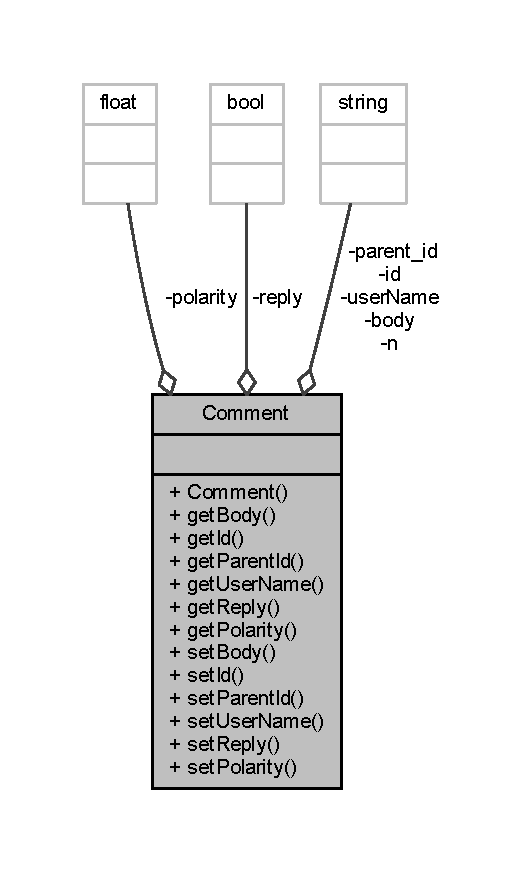
\includegraphics[width=252pt]{class_comment__coll__graph}
\end{center}
\end{figure}
\subsection*{Public Member Functions}
\begin{DoxyCompactItemize}
\item 
\hyperlink{class_comment_aa72817b1d59ba65d90a924e0ca056bee}{Comment} (std\+::string n\+Body, std\+::string n\+Id, std\+::string n\+P\+\_\+\+Id, bool n\+Reply, float polar, std\+::string username)
\item 
std\+::string \hyperlink{class_comment_acd202bf4ef1b23aa8a11cae4af4b44b4}{get\+Body} ()
\item 
std\+::string \hyperlink{class_comment_ab46d905afeb79abd5caa6434c84020d8}{get\+Id} ()
\item 
std\+::string \hyperlink{class_comment_a2903eea46f56ee796715e4989d1745f1}{get\+Parent\+Id} ()
\item 
std\+::string \hyperlink{class_comment_a192b820f7ad3d8065437436eae4408c5}{get\+User\+Name} ()
\item 
bool \hyperlink{class_comment_a89cfdb81dd327cf01d4f0fbb1d6f3c44}{get\+Reply} ()
\item 
float \hyperlink{class_comment_ab8f639d0d25165885bfbf09d3469f2b0}{get\+Polarity} ()
\item 
void \hyperlink{class_comment_abadebf70476d2ac212154fd52df103e7}{set\+Body} (std\+::string n\+Body)
\item 
void \hyperlink{class_comment_abb43aa20506c1d6cdb54c6b62e2b0d9d}{set\+Id} (std\+::string n\+Id)
\item 
void \hyperlink{class_comment_ac08d6d07afad5663c1d6c5886c7be333}{set\+Parent\+Id} (std\+::string p\+Id)
\item 
void \hyperlink{class_comment_a9e47b4560fb5d4e8e9e254a23622c6d5}{set\+User\+Name} (std\+::string name)
\item 
void \hyperlink{class_comment_ae6c057526fb2d3b789dfe99a0450f134}{set\+Reply} (bool rep)
\item 
void \hyperlink{class_comment_aa980db478aa7780f1094854e4df1bf4c}{set\+Polarity} (float polar)
\end{DoxyCompactItemize}
\subsection*{Private Attributes}
\begin{DoxyCompactItemize}
\item 
std\+::string \hyperlink{class_comment_a28bb2d16cad342d68d84b184c4ce07ba}{n}
\item 
std\+::string \hyperlink{class_comment_af8df10ee9d38440d5c4d500ccc9f2519}{body}
\item 
std\+::string \hyperlink{class_comment_a63db6067036146247c4ab7f663d90369}{id}
\item 
std\+::string \hyperlink{class_comment_abc88c0f64df05cb3d29ad1c7aa1621c5}{parent\+\_\+id}
\item 
std\+::string \hyperlink{class_comment_ad477f53e20e76aa9352926f93ccc7a56}{user\+Name}
\item 
float \hyperlink{class_comment_a617b67425b39c1f5f1eb0ada3d4bbd74}{polarity}
\item 
bool \hyperlink{class_comment_a7b8ceeb67364d5e08299baeeff38ba03}{reply}
\end{DoxyCompactItemize}
\subsection*{Friends}
\begin{DoxyCompactItemize}
\item 
bool \hyperlink{class_comment_ac5edd8dbab6e9d702dcdde889b96c250}{operator==} (const \hyperlink{class_comment}{Comment} \&c1, const \hyperlink{class_comment}{Comment} \&c2)
\begin{DoxyCompactList}\small\item\em Custom comparison operator. \end{DoxyCompactList}\end{DoxyCompactItemize}


\subsection{Detailed Description}
Model representation for the comment object within the program 

Definition at line 10 of file Comment.\+h.



\subsection{Constructor \& Destructor Documentation}
\mbox{\Hypertarget{class_comment_aa72817b1d59ba65d90a924e0ca056bee}\label{class_comment_aa72817b1d59ba65d90a924e0ca056bee}} 
\index{Comment@{Comment}!Comment@{Comment}}
\index{Comment@{Comment}!Comment@{Comment}}
\subsubsection{\texorpdfstring{Comment()}{Comment()}}
{\footnotesize\ttfamily Comment\+::\+Comment (\begin{DoxyParamCaption}\item[{std\+::string}]{n\+Body,  }\item[{std\+::string}]{n\+Id,  }\item[{std\+::string}]{n\+P\+\_\+\+Id,  }\item[{bool}]{n\+Reply,  }\item[{float}]{polar,  }\item[{std\+::string}]{username }\end{DoxyParamCaption})}



Definition at line 3 of file Comment.\+cpp.


\begin{DoxyCode}
3                                                                                                            
         : 
4     \hyperlink{class_comment_af8df10ee9d38440d5c4d500ccc9f2519}{body}(nBody), \hyperlink{class_comment_a63db6067036146247c4ab7f663d90369}{id}(nId), \hyperlink{class_comment_abc88c0f64df05cb3d29ad1c7aa1621c5}{parent\_id}(nP\_Id), \hyperlink{class_comment_a7b8ceeb67364d5e08299baeeff38ba03}{reply}(nReply), 
      \hyperlink{class_comment_a617b67425b39c1f5f1eb0ada3d4bbd74}{polarity}(nPolar), \hyperlink{class_comment_ad477f53e20e76aa9352926f93ccc7a56}{userName}(username)\{\}
\end{DoxyCode}


\subsection{Member Function Documentation}
\mbox{\Hypertarget{class_comment_acd202bf4ef1b23aa8a11cae4af4b44b4}\label{class_comment_acd202bf4ef1b23aa8a11cae4af4b44b4}} 
\index{Comment@{Comment}!get\+Body@{get\+Body}}
\index{get\+Body@{get\+Body}!Comment@{Comment}}
\subsubsection{\texorpdfstring{get\+Body()}{getBody()}}
{\footnotesize\ttfamily std\+::string Comment\+::get\+Body (\begin{DoxyParamCaption}{ }\end{DoxyParamCaption})}



Definition at line 6 of file Comment.\+cpp.



References body.


\begin{DoxyCode}
7 \{
8     \textcolor{keywordflow}{return} \hyperlink{class_comment_af8df10ee9d38440d5c4d500ccc9f2519}{body};
9 \}
\end{DoxyCode}
\mbox{\Hypertarget{class_comment_ab46d905afeb79abd5caa6434c84020d8}\label{class_comment_ab46d905afeb79abd5caa6434c84020d8}} 
\index{Comment@{Comment}!get\+Id@{get\+Id}}
\index{get\+Id@{get\+Id}!Comment@{Comment}}
\subsubsection{\texorpdfstring{get\+Id()}{getId()}}
{\footnotesize\ttfamily std\+::string Comment\+::get\+Id (\begin{DoxyParamCaption}{ }\end{DoxyParamCaption})}



Definition at line 11 of file Comment.\+cpp.



References id.



Referenced by Comment\+Formatter\+::sort\+Comment\+List().


\begin{DoxyCode}
12 \{
13     \textcolor{keywordflow}{return} \hyperlink{class_comment_a63db6067036146247c4ab7f663d90369}{id};
14 \}
\end{DoxyCode}
\mbox{\Hypertarget{class_comment_a2903eea46f56ee796715e4989d1745f1}\label{class_comment_a2903eea46f56ee796715e4989d1745f1}} 
\index{Comment@{Comment}!get\+Parent\+Id@{get\+Parent\+Id}}
\index{get\+Parent\+Id@{get\+Parent\+Id}!Comment@{Comment}}
\subsubsection{\texorpdfstring{get\+Parent\+Id()}{getParentId()}}
{\footnotesize\ttfamily std\+::string Comment\+::get\+Parent\+Id (\begin{DoxyParamCaption}{ }\end{DoxyParamCaption})}



Definition at line 16 of file Comment.\+cpp.



References parent\+\_\+id.


\begin{DoxyCode}
17 \{
18     \textcolor{keywordflow}{return} \hyperlink{class_comment_abc88c0f64df05cb3d29ad1c7aa1621c5}{parent\_id};
19 \}
\end{DoxyCode}
\mbox{\Hypertarget{class_comment_ab8f639d0d25165885bfbf09d3469f2b0}\label{class_comment_ab8f639d0d25165885bfbf09d3469f2b0}} 
\index{Comment@{Comment}!get\+Polarity@{get\+Polarity}}
\index{get\+Polarity@{get\+Polarity}!Comment@{Comment}}
\subsubsection{\texorpdfstring{get\+Polarity()}{getPolarity()}}
{\footnotesize\ttfamily float Comment\+::get\+Polarity (\begin{DoxyParamCaption}{ }\end{DoxyParamCaption})}



Definition at line 26 of file Comment.\+cpp.



References polarity.


\begin{DoxyCode}
27 \{
28     \textcolor{keywordflow}{return} \hyperlink{class_comment_a617b67425b39c1f5f1eb0ada3d4bbd74}{polarity};
29 \}
\end{DoxyCode}
\mbox{\Hypertarget{class_comment_a89cfdb81dd327cf01d4f0fbb1d6f3c44}\label{class_comment_a89cfdb81dd327cf01d4f0fbb1d6f3c44}} 
\index{Comment@{Comment}!get\+Reply@{get\+Reply}}
\index{get\+Reply@{get\+Reply}!Comment@{Comment}}
\subsubsection{\texorpdfstring{get\+Reply()}{getReply()}}
{\footnotesize\ttfamily bool Comment\+::get\+Reply (\begin{DoxyParamCaption}{ }\end{DoxyParamCaption})}



Definition at line 21 of file Comment.\+cpp.



References reply.


\begin{DoxyCode}
22 \{
23     \textcolor{keywordflow}{return} \hyperlink{class_comment_a7b8ceeb67364d5e08299baeeff38ba03}{reply};
24 \}
\end{DoxyCode}
\mbox{\Hypertarget{class_comment_a192b820f7ad3d8065437436eae4408c5}\label{class_comment_a192b820f7ad3d8065437436eae4408c5}} 
\index{Comment@{Comment}!get\+User\+Name@{get\+User\+Name}}
\index{get\+User\+Name@{get\+User\+Name}!Comment@{Comment}}
\subsubsection{\texorpdfstring{get\+User\+Name()}{getUserName()}}
{\footnotesize\ttfamily std\+::string Comment\+::get\+User\+Name (\begin{DoxyParamCaption}{ }\end{DoxyParamCaption})}



Definition at line 56 of file Comment.\+cpp.



References user\+Name.


\begin{DoxyCode}
57 \{
58     \textcolor{keywordflow}{return} \hyperlink{class_comment_ad477f53e20e76aa9352926f93ccc7a56}{userName};
59 \}
\end{DoxyCode}
\mbox{\Hypertarget{class_comment_abadebf70476d2ac212154fd52df103e7}\label{class_comment_abadebf70476d2ac212154fd52df103e7}} 
\index{Comment@{Comment}!set\+Body@{set\+Body}}
\index{set\+Body@{set\+Body}!Comment@{Comment}}
\subsubsection{\texorpdfstring{set\+Body()}{setBody()}}
{\footnotesize\ttfamily void Comment\+::set\+Body (\begin{DoxyParamCaption}\item[{std\+::string}]{n\+Body }\end{DoxyParamCaption})}



Definition at line 31 of file Comment.\+cpp.



References body.


\begin{DoxyCode}
32 \{
33     \hyperlink{class_comment_af8df10ee9d38440d5c4d500ccc9f2519}{body} = nBody;
34 \}
\end{DoxyCode}
\mbox{\Hypertarget{class_comment_abb43aa20506c1d6cdb54c6b62e2b0d9d}\label{class_comment_abb43aa20506c1d6cdb54c6b62e2b0d9d}} 
\index{Comment@{Comment}!set\+Id@{set\+Id}}
\index{set\+Id@{set\+Id}!Comment@{Comment}}
\subsubsection{\texorpdfstring{set\+Id()}{setId()}}
{\footnotesize\ttfamily void Comment\+::set\+Id (\begin{DoxyParamCaption}\item[{std\+::string}]{n\+Id }\end{DoxyParamCaption})}



Definition at line 36 of file Comment.\+cpp.


\begin{DoxyCode}
37 \{
38     \textcolor{keywordtype}{id} = nId;
39 \}
\end{DoxyCode}
\mbox{\Hypertarget{class_comment_ac08d6d07afad5663c1d6c5886c7be333}\label{class_comment_ac08d6d07afad5663c1d6c5886c7be333}} 
\index{Comment@{Comment}!set\+Parent\+Id@{set\+Parent\+Id}}
\index{set\+Parent\+Id@{set\+Parent\+Id}!Comment@{Comment}}
\subsubsection{\texorpdfstring{set\+Parent\+Id()}{setParentId()}}
{\footnotesize\ttfamily void Comment\+::set\+Parent\+Id (\begin{DoxyParamCaption}\item[{std\+::string}]{p\+Id }\end{DoxyParamCaption})}



Definition at line 41 of file Comment.\+cpp.



References parent\+\_\+id.


\begin{DoxyCode}
42 \{
43     \hyperlink{class_comment_abc88c0f64df05cb3d29ad1c7aa1621c5}{parent\_id} = nP\_Id;
44 \}
\end{DoxyCode}
\mbox{\Hypertarget{class_comment_aa980db478aa7780f1094854e4df1bf4c}\label{class_comment_aa980db478aa7780f1094854e4df1bf4c}} 
\index{Comment@{Comment}!set\+Polarity@{set\+Polarity}}
\index{set\+Polarity@{set\+Polarity}!Comment@{Comment}}
\subsubsection{\texorpdfstring{set\+Polarity()}{setPolarity()}}
{\footnotesize\ttfamily void Comment\+::set\+Polarity (\begin{DoxyParamCaption}\item[{float}]{polar }\end{DoxyParamCaption})}



Definition at line 51 of file Comment.\+cpp.



References polarity.


\begin{DoxyCode}
52 \{
53     \hyperlink{class_comment_a617b67425b39c1f5f1eb0ada3d4bbd74}{polarity} = polar;
54 \}
\end{DoxyCode}
\mbox{\Hypertarget{class_comment_ae6c057526fb2d3b789dfe99a0450f134}\label{class_comment_ae6c057526fb2d3b789dfe99a0450f134}} 
\index{Comment@{Comment}!set\+Reply@{set\+Reply}}
\index{set\+Reply@{set\+Reply}!Comment@{Comment}}
\subsubsection{\texorpdfstring{set\+Reply()}{setReply()}}
{\footnotesize\ttfamily void Comment\+::set\+Reply (\begin{DoxyParamCaption}\item[{bool}]{rep }\end{DoxyParamCaption})}



Definition at line 46 of file Comment.\+cpp.



References reply.


\begin{DoxyCode}
47 \{
48     \hyperlink{class_comment_a7b8ceeb67364d5e08299baeeff38ba03}{reply} = nReply;
49 \}
\end{DoxyCode}
\mbox{\Hypertarget{class_comment_a9e47b4560fb5d4e8e9e254a23622c6d5}\label{class_comment_a9e47b4560fb5d4e8e9e254a23622c6d5}} 
\index{Comment@{Comment}!set\+User\+Name@{set\+User\+Name}}
\index{set\+User\+Name@{set\+User\+Name}!Comment@{Comment}}
\subsubsection{\texorpdfstring{set\+User\+Name()}{setUserName()}}
{\footnotesize\ttfamily void Comment\+::set\+User\+Name (\begin{DoxyParamCaption}\item[{std\+::string}]{name }\end{DoxyParamCaption})}



Definition at line 61 of file Comment.\+cpp.



References user\+Name.


\begin{DoxyCode}
62 \{
63     \hyperlink{class_comment_ad477f53e20e76aa9352926f93ccc7a56}{userName} = name;
64 \}
\end{DoxyCode}


\subsection{Friends And Related Function Documentation}
\mbox{\Hypertarget{class_comment_ac5edd8dbab6e9d702dcdde889b96c250}\label{class_comment_ac5edd8dbab6e9d702dcdde889b96c250}} 
\index{Comment@{Comment}!operator==@{operator==}}
\index{operator==@{operator==}!Comment@{Comment}}
\subsubsection{\texorpdfstring{operator==}{operator==}}
{\footnotesize\ttfamily bool operator== (\begin{DoxyParamCaption}\item[{const \hyperlink{class_comment}{Comment} \&}]{c1,  }\item[{const \hyperlink{class_comment}{Comment} \&}]{c2 }\end{DoxyParamCaption})\hspace{0.3cm}{\ttfamily [friend]}}



Custom comparison operator. 



Definition at line 66 of file Comment.\+cpp.


\begin{DoxyCode}
67 \{
68     \textcolor{keywordflow}{return} (c1.\hyperlink{class_comment_a63db6067036146247c4ab7f663d90369}{id} == c2.\hyperlink{class_comment_a63db6067036146247c4ab7f663d90369}{id}) && (c1.\hyperlink{class_comment_af8df10ee9d38440d5c4d500ccc9f2519}{body} == c2.\hyperlink{class_comment_af8df10ee9d38440d5c4d500ccc9f2519}{body}) && (c1.\hyperlink{class_comment_abc88c0f64df05cb3d29ad1c7aa1621c5}{parent\_id} == c2.
      \hyperlink{class_comment_abc88c0f64df05cb3d29ad1c7aa1621c5}{parent\_id}) && (c1.\hyperlink{class_comment_a617b67425b39c1f5f1eb0ada3d4bbd74}{polarity} == c2.\hyperlink{class_comment_a617b67425b39c1f5f1eb0ada3d4bbd74}{polarity}) && (c1.\hyperlink{class_comment_a7b8ceeb67364d5e08299baeeff38ba03}{reply} == c2.
      \hyperlink{class_comment_a7b8ceeb67364d5e08299baeeff38ba03}{reply});
69 \}
\end{DoxyCode}


\subsection{Member Data Documentation}
\mbox{\Hypertarget{class_comment_af8df10ee9d38440d5c4d500ccc9f2519}\label{class_comment_af8df10ee9d38440d5c4d500ccc9f2519}} 
\index{Comment@{Comment}!body@{body}}
\index{body@{body}!Comment@{Comment}}
\subsubsection{\texorpdfstring{body}{body}}
{\footnotesize\ttfamily std\+::string Comment\+::body\hspace{0.3cm}{\ttfamily [private]}}



Definition at line 35 of file Comment.\+h.



Referenced by get\+Body(), operator==(), and set\+Body().

\mbox{\Hypertarget{class_comment_a63db6067036146247c4ab7f663d90369}\label{class_comment_a63db6067036146247c4ab7f663d90369}} 
\index{Comment@{Comment}!id@{id}}
\index{id@{id}!Comment@{Comment}}
\subsubsection{\texorpdfstring{id}{id}}
{\footnotesize\ttfamily std\+::string Comment\+::id\hspace{0.3cm}{\ttfamily [private]}}



Definition at line 36 of file Comment.\+h.



Referenced by get\+Id(), and operator==().

\mbox{\Hypertarget{class_comment_a28bb2d16cad342d68d84b184c4ce07ba}\label{class_comment_a28bb2d16cad342d68d84b184c4ce07ba}} 
\index{Comment@{Comment}!n@{n}}
\index{n@{n}!Comment@{Comment}}
\subsubsection{\texorpdfstring{n}{n}}
{\footnotesize\ttfamily std\+::string Comment\+::n\hspace{0.3cm}{\ttfamily [private]}}



Definition at line 34 of file Comment.\+h.

\mbox{\Hypertarget{class_comment_abc88c0f64df05cb3d29ad1c7aa1621c5}\label{class_comment_abc88c0f64df05cb3d29ad1c7aa1621c5}} 
\index{Comment@{Comment}!parent\+\_\+id@{parent\+\_\+id}}
\index{parent\+\_\+id@{parent\+\_\+id}!Comment@{Comment}}
\subsubsection{\texorpdfstring{parent\+\_\+id}{parent\_id}}
{\footnotesize\ttfamily std\+::string Comment\+::parent\+\_\+id\hspace{0.3cm}{\ttfamily [private]}}



Definition at line 37 of file Comment.\+h.



Referenced by get\+Parent\+Id(), operator==(), and set\+Parent\+Id().

\mbox{\Hypertarget{class_comment_a617b67425b39c1f5f1eb0ada3d4bbd74}\label{class_comment_a617b67425b39c1f5f1eb0ada3d4bbd74}} 
\index{Comment@{Comment}!polarity@{polarity}}
\index{polarity@{polarity}!Comment@{Comment}}
\subsubsection{\texorpdfstring{polarity}{polarity}}
{\footnotesize\ttfamily float Comment\+::polarity\hspace{0.3cm}{\ttfamily [private]}}



Definition at line 39 of file Comment.\+h.



Referenced by get\+Polarity(), operator==(), and set\+Polarity().

\mbox{\Hypertarget{class_comment_a7b8ceeb67364d5e08299baeeff38ba03}\label{class_comment_a7b8ceeb67364d5e08299baeeff38ba03}} 
\index{Comment@{Comment}!reply@{reply}}
\index{reply@{reply}!Comment@{Comment}}
\subsubsection{\texorpdfstring{reply}{reply}}
{\footnotesize\ttfamily bool Comment\+::reply\hspace{0.3cm}{\ttfamily [private]}}



Definition at line 40 of file Comment.\+h.



Referenced by get\+Reply(), operator==(), and set\+Reply().

\mbox{\Hypertarget{class_comment_ad477f53e20e76aa9352926f93ccc7a56}\label{class_comment_ad477f53e20e76aa9352926f93ccc7a56}} 
\index{Comment@{Comment}!user\+Name@{user\+Name}}
\index{user\+Name@{user\+Name}!Comment@{Comment}}
\subsubsection{\texorpdfstring{user\+Name}{userName}}
{\footnotesize\ttfamily std\+::string Comment\+::user\+Name\hspace{0.3cm}{\ttfamily [private]}}



Definition at line 38 of file Comment.\+h.



Referenced by get\+User\+Name(), and set\+User\+Name().



The documentation for this class was generated from the following files\+:\begin{DoxyCompactItemize}
\item 
C\+:/\+Users/\+Kyle Tuckey/\+Documents/\+Final Year Project/\+Social\+\_\+\+N\+P\+C\+S/\+Social\+\_\+\+N\+P\+C\+S/\hyperlink{_comment_8h}{Comment.\+h}\item 
C\+:/\+Users/\+Kyle Tuckey/\+Documents/\+Final Year Project/\+Social\+\_\+\+N\+P\+C\+S/\+Social\+\_\+\+N\+P\+C\+S/\hyperlink{_comment_8cpp}{Comment.\+cpp}\end{DoxyCompactItemize}

\hypertarget{class_comment_formatter}{}\section{Comment\+Formatter Class Reference}
\label{class_comment_formatter}\index{Comment\+Formatter@{Comment\+Formatter}}


{\ttfamily \#include $<$Comment\+Formatter.\+h$>$}



Collaboration diagram for Comment\+Formatter\+:\nopagebreak
\begin{figure}[H]
\begin{center}
\leavevmode
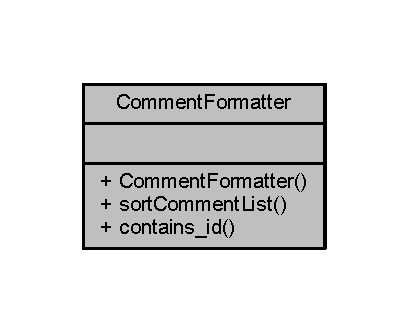
\includegraphics[width=196pt]{class_comment_formatter__coll__graph}
\end{center}
\end{figure}
\subsection*{Public Member Functions}
\begin{DoxyCompactItemize}
\item 
\hyperlink{class_comment_formatter_a2109e1c890568fbc960c06605d30563e}{Comment\+Formatter} ()
\item 
std\+::vector$<$ \hyperlink{class_comment}{Comment} $>$ \hyperlink{class_comment_formatter_a6a9af9cdde666a914d97c3f45e6c8a49}{sort\+Comment\+List} (\hyperlink{class_comment}{Comment} com, std\+::vector$<$ \hyperlink{class_comment}{Comment} $>$ coms, std\+::vector$<$ \hyperlink{class_comment}{Comment} $>$ n\+Coms, int maximum)
\item 
bool \hyperlink{class_comment_formatter_a3ee22833399687c24694b6e11a3337ba}{contains\+\_\+id} (const std\+::string \&parent\+\_\+id, const std\+::string \&id)
\end{DoxyCompactItemize}


\subsection{Detailed Description}
The comment formatter sorts the a list of comments by comment-\/$>$reply-\/$>$reply... 

Definition at line 9 of file Comment\+Formatter.\+h.



\subsection{Constructor \& Destructor Documentation}
\mbox{\Hypertarget{class_comment_formatter_a2109e1c890568fbc960c06605d30563e}\label{class_comment_formatter_a2109e1c890568fbc960c06605d30563e}} 
\index{Comment\+Formatter@{Comment\+Formatter}!Comment\+Formatter@{Comment\+Formatter}}
\index{Comment\+Formatter@{Comment\+Formatter}!Comment\+Formatter@{Comment\+Formatter}}
\subsubsection{\texorpdfstring{Comment\+Formatter()}{CommentFormatter()}}
{\footnotesize\ttfamily Comment\+Formatter\+::\+Comment\+Formatter (\begin{DoxyParamCaption}{ }\end{DoxyParamCaption})}



Definition at line 3 of file Comment\+Formatter.\+cpp.


\begin{DoxyCode}
4 \{
5 \}
\end{DoxyCode}


\subsection{Member Function Documentation}
\mbox{\Hypertarget{class_comment_formatter_a3ee22833399687c24694b6e11a3337ba}\label{class_comment_formatter_a3ee22833399687c24694b6e11a3337ba}} 
\index{Comment\+Formatter@{Comment\+Formatter}!contains\+\_\+id@{contains\+\_\+id}}
\index{contains\+\_\+id@{contains\+\_\+id}!Comment\+Formatter@{Comment\+Formatter}}
\subsubsection{\texorpdfstring{contains\+\_\+id()}{contains\_id()}}
{\footnotesize\ttfamily bool Comment\+Formatter\+::contains\+\_\+id (\begin{DoxyParamCaption}\item[{const std\+::string \&}]{parent\+\_\+id,  }\item[{const std\+::string \&}]{id }\end{DoxyParamCaption})}



Definition at line 46 of file Comment\+Formatter.\+cpp.



Referenced by sort\+Comment\+List().


\begin{DoxyCode}
47 \{
48     \textcolor{keywordtype}{size\_t} pos = 0;
49     \textcolor{keywordflow}{while} ((pos = parent\_id.substr(pos).find(\textcolor{keywordtype}{id})) != std::string::npos)
50     \{
51         \textcolor{keywordflow}{if} (!(isalpha(parent\_id[pos - 1])) || !(isalpha(parent\_id[pos + \textcolor{keywordtype}{id}.size() + 1])))
52             \textcolor{keywordflow}{return} \textcolor{keyword}{true};
53     \}
54     \textcolor{keywordflow}{return} \textcolor{keyword}{false};
55 \}
\end{DoxyCode}
\mbox{\Hypertarget{class_comment_formatter_a6a9af9cdde666a914d97c3f45e6c8a49}\label{class_comment_formatter_a6a9af9cdde666a914d97c3f45e6c8a49}} 
\index{Comment\+Formatter@{Comment\+Formatter}!sort\+Comment\+List@{sort\+Comment\+List}}
\index{sort\+Comment\+List@{sort\+Comment\+List}!Comment\+Formatter@{Comment\+Formatter}}
\subsubsection{\texorpdfstring{sort\+Comment\+List()}{sortCommentList()}}
{\footnotesize\ttfamily std\+::vector$<$ \hyperlink{class_comment}{Comment} $>$ Comment\+Formatter\+::sort\+Comment\+List (\begin{DoxyParamCaption}\item[{\hyperlink{class_comment}{Comment}}]{com,  }\item[{std\+::vector$<$ \hyperlink{class_comment}{Comment} $>$}]{coms,  }\item[{std\+::vector$<$ \hyperlink{class_comment}{Comment} $>$}]{n\+Coms,  }\item[{int}]{maximum }\end{DoxyParamCaption})}



Definition at line 11 of file Comment\+Formatter.\+cpp.



References contains\+\_\+id(), and Comment\+::get\+Id().



Referenced by Group\+Populator\+::\+Populate\+Group().


\begin{DoxyCode}
12 \{
13     \textcolor{comment}{//we only want to do this when nComs is less than the maximum given value}
14     \textcolor{keywordflow}{if} (nComs.size() < maximum) \{
15 
16         \textcolor{comment}{//push back the current comment}
17         nComs.push\_back(com);
18 
19         \textcolor{comment}{//erase the comment from coms, this is so that we do not go beyond the index range of coms, and to
       avoid adding duplicates}
20         coms.erase(std::remove(coms.begin(), coms.end(), com), coms.end());
21         \textcolor{keywordflow}{for} (\textcolor{keywordtype}{int} i = 0; i < coms.size(); i++)
22         \{
23             \textcolor{comment}{//we check to see if a comment contain's the id of com in it's parent\_id, if it does, then it
       is a reply to that comment}
24             \textcolor{keywordflow}{if} (\hyperlink{class_comment_formatter_a3ee22833399687c24694b6e11a3337ba}{contains\_id}(coms[i].getParentId(), com.\hyperlink{class_comment_ab46d905afeb79abd5caa6434c84020d8}{getId}())) \{
25                 \hyperlink{class_comment}{Comment} cRep = coms[i];
26 
27                 \textcolor{comment}{//remove the reply from the comments array}
28                 coms.erase(std::remove(coms.begin(), coms.end(), coms[i]), coms.end());
29 
30                 \textcolor{comment}{//parse the reply into this function along with our current value's, this is so that we can
       find any reply's for the reply itself}
31                 nComs = \hyperlink{class_comment_formatter_a6a9af9cdde666a914d97c3f45e6c8a49}{sortCommentList}(cRep, coms, nComs, maximum);
32             \}
33         \}
34 
35         \textcolor{comment}{//if the size of com's is not 0, then there are still comments we have not sorted so we call the
       function again.}
36         \textcolor{keywordflow}{if}(coms.size() != 0)
37             nComs = \hyperlink{class_comment_formatter_a6a9af9cdde666a914d97c3f45e6c8a49}{sortCommentList}(coms[0], coms, nComs, maximum);
38     \}
39     \textcolor{keywordflow}{return} nComs;
40 \}
\end{DoxyCode}


The documentation for this class was generated from the following files\+:\begin{DoxyCompactItemize}
\item 
C\+:/\+Users/\+Kyle Tuckey/\+Documents/\+Final Year Project/\+Social\+\_\+\+N\+P\+C\+S/\+Social\+\_\+\+N\+P\+C\+S/\hyperlink{_comment_formatter_8h}{Comment\+Formatter.\+h}\item 
C\+:/\+Users/\+Kyle Tuckey/\+Documents/\+Final Year Project/\+Social\+\_\+\+N\+P\+C\+S/\+Social\+\_\+\+N\+P\+C\+S/\hyperlink{_comment_formatter_8cpp}{Comment\+Formatter.\+cpp}\end{DoxyCompactItemize}

\hypertarget{class_group}{}\section{Group Class Reference}
\label{class_group}\index{Group@{Group}}


{\ttfamily \#include $<$Group.\+h$>$}



Collaboration diagram for Group\+:\nopagebreak
\begin{figure}[H]
\begin{center}
\leavevmode
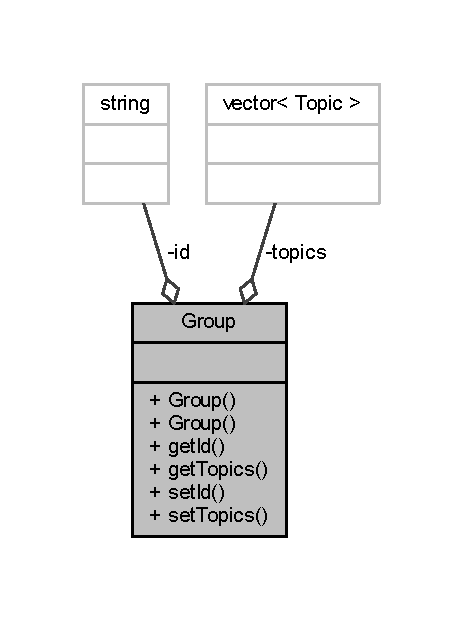
\includegraphics[width=222pt]{class_group__coll__graph}
\end{center}
\end{figure}
\subsection*{Public Member Functions}
\begin{DoxyCompactItemize}
\item 
\hyperlink{class_group_a7b74f9ac68e0504ccf2e2854b7355ff1}{Group} ()
\item 
\hyperlink{class_group_ac3639ca791bff4ceeaeba9e3fe4c1835}{Group} (std\+::string n\+Id, std\+::vector$<$ \hyperlink{class_topic}{Topic} $>$ n\+Topics)
\item 
std\+::string \hyperlink{class_group_ac28178935f780582ce7f5f518d43b6f8}{get\+Id} ()
\item 
std\+::vector$<$ \hyperlink{class_topic}{Topic} $>$ \hyperlink{class_group_a160daa5f96a8203bd30340dfc1810af1}{get\+Topics} ()
\item 
void \hyperlink{class_group_aba314538b0284ebfdf2e89fcdeef8697}{set\+Id} (std\+::string n\+Id)
\item 
void \hyperlink{class_group_ab37f8ac624dedf6eb84e2603e9c51df2}{set\+Topics} (std\+::vector$<$ \hyperlink{class_topic}{Topic} $>$ n\+Topics)
\end{DoxyCompactItemize}
\subsection*{Private Attributes}
\begin{DoxyCompactItemize}
\item 
std\+::string \hyperlink{class_group_ade135fec88f463adb44f780cb476e7d3}{id}
\item 
std\+::vector$<$ \hyperlink{class_topic}{Topic} $>$ \hyperlink{class_group_a5927c259318d2058c9d1573110718bb5}{topics}
\end{DoxyCompactItemize}
\subsection*{Friends}
\begin{DoxyCompactItemize}
\item 
bool \hyperlink{class_group_a5127806edb762fcce6c5450dcb17a395}{operator==} (const \hyperlink{class_group}{Group} \&c1, const \hyperlink{class_group}{Group} \&c2)
\begin{DoxyCompactList}\small\item\em Custom compare operator. \end{DoxyCompactList}\end{DoxyCompactItemize}


\subsection{Detailed Description}
Model representation for the \hyperlink{class_group}{Group} object within the program 

Definition at line 6 of file Group.\+h.



\subsection{Constructor \& Destructor Documentation}
\mbox{\Hypertarget{class_group_a7b74f9ac68e0504ccf2e2854b7355ff1}\label{class_group_a7b74f9ac68e0504ccf2e2854b7355ff1}} 
\index{Group@{Group}!Group@{Group}}
\index{Group@{Group}!Group@{Group}}
\subsubsection{\texorpdfstring{Group()}{Group()}\hspace{0.1cm}{\footnotesize\ttfamily [1/2]}}
{\footnotesize\ttfamily Group\+::\+Group (\begin{DoxyParamCaption}{ }\end{DoxyParamCaption})}



Definition at line 3 of file Group.\+cpp.


\begin{DoxyCode}
3 \{\}
\end{DoxyCode}
\mbox{\Hypertarget{class_group_ac3639ca791bff4ceeaeba9e3fe4c1835}\label{class_group_ac3639ca791bff4ceeaeba9e3fe4c1835}} 
\index{Group@{Group}!Group@{Group}}
\index{Group@{Group}!Group@{Group}}
\subsubsection{\texorpdfstring{Group()}{Group()}\hspace{0.1cm}{\footnotesize\ttfamily [2/2]}}
{\footnotesize\ttfamily Group\+::\+Group (\begin{DoxyParamCaption}\item[{std\+::string}]{n\+Id,  }\item[{std\+::vector$<$ \hyperlink{class_topic}{Topic} $>$}]{n\+Topics }\end{DoxyParamCaption})}



Definition at line 5 of file Group.\+cpp.



References set\+Id(), and set\+Topics().


\begin{DoxyCode}
6 \{
7     \hyperlink{class_group_aba314538b0284ebfdf2e89fcdeef8697}{setId}(nId);
8     \hyperlink{class_group_ab37f8ac624dedf6eb84e2603e9c51df2}{setTopics}(nTopics);
9 \}
\end{DoxyCode}


\subsection{Member Function Documentation}
\mbox{\Hypertarget{class_group_ac28178935f780582ce7f5f518d43b6f8}\label{class_group_ac28178935f780582ce7f5f518d43b6f8}} 
\index{Group@{Group}!get\+Id@{get\+Id}}
\index{get\+Id@{get\+Id}!Group@{Group}}
\subsubsection{\texorpdfstring{get\+Id()}{getId()}}
{\footnotesize\ttfamily std\+::string Group\+::get\+Id (\begin{DoxyParamCaption}{ }\end{DoxyParamCaption})}



Definition at line 11 of file Group.\+cpp.



References id.


\begin{DoxyCode}
12 \{
13     \textcolor{keywordflow}{return} \hyperlink{class_group_ade135fec88f463adb44f780cb476e7d3}{id};
14 \}
\end{DoxyCode}
\mbox{\Hypertarget{class_group_a160daa5f96a8203bd30340dfc1810af1}\label{class_group_a160daa5f96a8203bd30340dfc1810af1}} 
\index{Group@{Group}!get\+Topics@{get\+Topics}}
\index{get\+Topics@{get\+Topics}!Group@{Group}}
\subsubsection{\texorpdfstring{get\+Topics()}{getTopics()}}
{\footnotesize\ttfamily std\+::vector$<$ \hyperlink{class_topic}{Topic} $>$ Group\+::get\+Topics (\begin{DoxyParamCaption}{ }\end{DoxyParamCaption})}



Definition at line 16 of file Group.\+cpp.



References topics.



Referenced by Room\+::\+Room().


\begin{DoxyCode}
17 \{
18     \textcolor{keywordflow}{return} \hyperlink{class_group_a5927c259318d2058c9d1573110718bb5}{topics};
19 \}
\end{DoxyCode}
\mbox{\Hypertarget{class_group_aba314538b0284ebfdf2e89fcdeef8697}\label{class_group_aba314538b0284ebfdf2e89fcdeef8697}} 
\index{Group@{Group}!set\+Id@{set\+Id}}
\index{set\+Id@{set\+Id}!Group@{Group}}
\subsubsection{\texorpdfstring{set\+Id()}{setId()}}
{\footnotesize\ttfamily void Group\+::set\+Id (\begin{DoxyParamCaption}\item[{std\+::string}]{n\+Id }\end{DoxyParamCaption})}



Definition at line 21 of file Group.\+cpp.



Referenced by Group().


\begin{DoxyCode}
22 \{
23     \textcolor{keywordtype}{id} = nId;
24 \}
\end{DoxyCode}
\mbox{\Hypertarget{class_group_ab37f8ac624dedf6eb84e2603e9c51df2}\label{class_group_ab37f8ac624dedf6eb84e2603e9c51df2}} 
\index{Group@{Group}!set\+Topics@{set\+Topics}}
\index{set\+Topics@{set\+Topics}!Group@{Group}}
\subsubsection{\texorpdfstring{set\+Topics()}{setTopics()}}
{\footnotesize\ttfamily void Group\+::set\+Topics (\begin{DoxyParamCaption}\item[{std\+::vector$<$ \hyperlink{class_topic}{Topic} $>$}]{n\+Topics }\end{DoxyParamCaption})}



Definition at line 26 of file Group.\+cpp.



References topics.



Referenced by Group().


\begin{DoxyCode}
27 \{
28     \hyperlink{class_group_a5927c259318d2058c9d1573110718bb5}{topics} = nTopics;
29 \}
\end{DoxyCode}


\subsection{Friends And Related Function Documentation}
\mbox{\Hypertarget{class_group_a5127806edb762fcce6c5450dcb17a395}\label{class_group_a5127806edb762fcce6c5450dcb17a395}} 
\index{Group@{Group}!operator==@{operator==}}
\index{operator==@{operator==}!Group@{Group}}
\subsubsection{\texorpdfstring{operator==}{operator==}}
{\footnotesize\ttfamily bool operator== (\begin{DoxyParamCaption}\item[{const \hyperlink{class_group}{Group} \&}]{c1,  }\item[{const \hyperlink{class_group}{Group} \&}]{c2 }\end{DoxyParamCaption})\hspace{0.3cm}{\ttfamily [friend]}}



Custom compare operator. 



Definition at line 31 of file Group.\+cpp.


\begin{DoxyCode}
32 \{
33     \textcolor{keywordflow}{return}  (t1.id == t2.id) && (t1.topics == t2.topics);
34 \}
\end{DoxyCode}


\subsection{Member Data Documentation}
\mbox{\Hypertarget{class_group_ade135fec88f463adb44f780cb476e7d3}\label{class_group_ade135fec88f463adb44f780cb476e7d3}} 
\index{Group@{Group}!id@{id}}
\index{id@{id}!Group@{Group}}
\subsubsection{\texorpdfstring{id}{id}}
{\footnotesize\ttfamily std\+::string Group\+::id\hspace{0.3cm}{\ttfamily [private]}}



Definition at line 21 of file Group.\+h.



Referenced by get\+Id(), and operator==().

\mbox{\Hypertarget{class_group_a5927c259318d2058c9d1573110718bb5}\label{class_group_a5927c259318d2058c9d1573110718bb5}} 
\index{Group@{Group}!topics@{topics}}
\index{topics@{topics}!Group@{Group}}
\subsubsection{\texorpdfstring{topics}{topics}}
{\footnotesize\ttfamily std\+::vector$<$\hyperlink{class_topic}{Topic}$>$ Group\+::topics\hspace{0.3cm}{\ttfamily [private]}}



Definition at line 22 of file Group.\+h.



Referenced by get\+Topics(), operator==(), and set\+Topics().



The documentation for this class was generated from the following files\+:\begin{DoxyCompactItemize}
\item 
C\+:/\+Users/\+Kyle Tuckey/\+Documents/\+Final Year Project/\+Social\+\_\+\+N\+P\+C\+S/\+Social\+\_\+\+N\+P\+C\+S/\hyperlink{_group_8h}{Group.\+h}\item 
C\+:/\+Users/\+Kyle Tuckey/\+Documents/\+Final Year Project/\+Social\+\_\+\+N\+P\+C\+S/\+Social\+\_\+\+N\+P\+C\+S/\hyperlink{_group_8cpp}{Group.\+cpp}\end{DoxyCompactItemize}

\hypertarget{class_group_populator}{}\section{Group\+Populator Class Reference}
\label{class_group_populator}\index{Group\+Populator@{Group\+Populator}}


{\ttfamily \#include $<$Group\+Populator.\+h$>$}



Collaboration diagram for Group\+Populator\+:\nopagebreak
\begin{figure}[H]
\begin{center}
\leavevmode
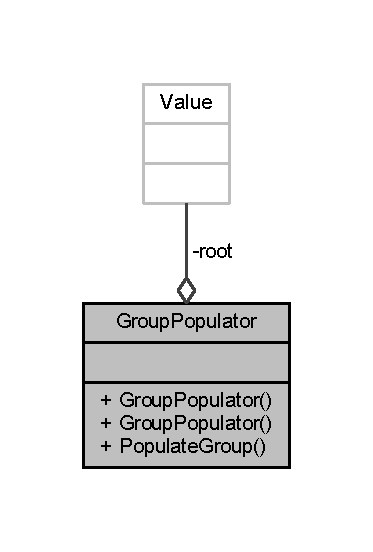
\includegraphics[width=179pt]{class_group_populator__coll__graph}
\end{center}
\end{figure}
\subsection*{Public Member Functions}
\begin{DoxyCompactItemize}
\item 
\hyperlink{class_group_populator_a90814524b9b87b4841bdc64f3c7e56ef}{Group\+Populator} (std\+::ifstream file)
\item 
\hyperlink{class_group_populator_a8d125db2718e9d7bb70699094045f43b}{Group\+Populator} ()
\item 
\hyperlink{class_group}{Group} \hyperlink{class_group_populator_ae4c9f15b1d55f61497c97140df8af0b7}{Populate\+Group} ()
\begin{DoxyCompactList}\small\item\em returns a populated group object \end{DoxyCompactList}\end{DoxyCompactItemize}
\subsection*{Private Attributes}
\begin{DoxyCompactItemize}
\item 
Json\+::\+Value \hyperlink{class_group_populator_a161f0427ec538d3a99da2e53fdbc9b2b}{root}
\end{DoxyCompactItemize}


\subsection{Detailed Description}
Populates the group object with data parsed into the contructor 

Definition at line 10 of file Group\+Populator.\+h.



\subsection{Constructor \& Destructor Documentation}
\mbox{\Hypertarget{class_group_populator_a90814524b9b87b4841bdc64f3c7e56ef}\label{class_group_populator_a90814524b9b87b4841bdc64f3c7e56ef}} 
\index{Group\+Populator@{Group\+Populator}!Group\+Populator@{Group\+Populator}}
\index{Group\+Populator@{Group\+Populator}!Group\+Populator@{Group\+Populator}}
\subsubsection{\texorpdfstring{Group\+Populator()}{GroupPopulator()}\hspace{0.1cm}{\footnotesize\ttfamily [1/2]}}
{\footnotesize\ttfamily Group\+Populator\+::\+Group\+Populator (\begin{DoxyParamCaption}\item[{std\+::ifstream}]{file }\end{DoxyParamCaption})}



Definition at line 9 of file Group\+Populator.\+cpp.



References root.


\begin{DoxyCode}
10 \{
11     file >> \hyperlink{class_group_populator_a161f0427ec538d3a99da2e53fdbc9b2b}{root};
12 \}
\end{DoxyCode}
\mbox{\Hypertarget{class_group_populator_a8d125db2718e9d7bb70699094045f43b}\label{class_group_populator_a8d125db2718e9d7bb70699094045f43b}} 
\index{Group\+Populator@{Group\+Populator}!Group\+Populator@{Group\+Populator}}
\index{Group\+Populator@{Group\+Populator}!Group\+Populator@{Group\+Populator}}
\subsubsection{\texorpdfstring{Group\+Populator()}{GroupPopulator()}\hspace{0.1cm}{\footnotesize\ttfamily [2/2]}}
{\footnotesize\ttfamily Group\+Populator\+::\+Group\+Populator (\begin{DoxyParamCaption}{ }\end{DoxyParamCaption})}



Definition at line 4 of file Group\+Populator.\+cpp.


\begin{DoxyCode}
5 \{
6 
7 \}
\end{DoxyCode}


\subsection{Member Function Documentation}
\mbox{\Hypertarget{class_group_populator_ae4c9f15b1d55f61497c97140df8af0b7}\label{class_group_populator_ae4c9f15b1d55f61497c97140df8af0b7}} 
\index{Group\+Populator@{Group\+Populator}!Populate\+Group@{Populate\+Group}}
\index{Populate\+Group@{Populate\+Group}!Group\+Populator@{Group\+Populator}}
\subsubsection{\texorpdfstring{Populate\+Group()}{PopulateGroup()}}
{\footnotesize\ttfamily \hyperlink{class_group}{Group} Group\+Populator\+::\+Populate\+Group (\begin{DoxyParamCaption}{ }\end{DoxyParamCaption})}



returns a populated group object 

access\textquotesingle{}s the read in J\+S\+ON file to populate our group object 

Definition at line 17 of file Group\+Populator.\+cpp.



References root, and Comment\+Formatter\+::sort\+Comment\+List().


\begin{DoxyCode}
18 \{
19     std::vector<Topic> nTops;
20     \hyperlink{class_comment_formatter}{CommentFormatter} cfrm;
21     std::vector<Comment> a;
22 
23     \textcolor{comment}{// access each 'topics' value in the JSON file}
24     \textcolor{keywordflow}{for} (\textcolor{keyword}{const} Json::Value& tops : \hyperlink{class_group_populator_a161f0427ec538d3a99da2e53fdbc9b2b}{root}[\textcolor{stringliteral}{"topics"}])
25     \{
26         std::vector<Comment> nComms;
27 
28         \textcolor{comment}{// acess each 'comments' value in the JSON file}
29         \textcolor{keywordflow}{for} (\textcolor{keyword}{const} Json::Value& comms : tops[\textcolor{stringliteral}{"comments"}])
30         \{
31             \hyperlink{class_comment}{Comment} com(comms[\textcolor{stringliteral}{"body"}].asString(), comms[\textcolor{stringliteral}{"id"}].asString(), comms[\textcolor{stringliteral}{"parent\_id"}].
      asString(), 
32                 comms[\textcolor{stringliteral}{"reply"}].asBool(), comms[\textcolor{stringliteral}{"polarity"}].asFloat(), comms[\textcolor{stringliteral}{"author"}].asString());
33             nComms.push\_back(com);
34         \}
35 
36         \textcolor{comment}{// use the comment formatter to format the list, then add it to the topic}
37         nComms = cfrm.\hyperlink{class_comment_formatter_a6a9af9cdde666a914d97c3f45e6c8a49}{sortCommentList}(nComms[0], nComms, a, nComms.size());
38         \hyperlink{class_topic}{Topic} top(tops[\textcolor{stringliteral}{"id"}].asString(), tops[\textcolor{stringliteral}{"topic"}].asString(), nComms);
39 
40         \textcolor{comment}{// add the topic to the group}
41         nTops.push\_back(top);
42     \}
43     \textcolor{keywordflow}{return} \hyperlink{class_group}{Group}(root[\textcolor{stringliteral}{"subject"}].asString(), nTops);
44 \}
\end{DoxyCode}


\subsection{Member Data Documentation}
\mbox{\Hypertarget{class_group_populator_a161f0427ec538d3a99da2e53fdbc9b2b}\label{class_group_populator_a161f0427ec538d3a99da2e53fdbc9b2b}} 
\index{Group\+Populator@{Group\+Populator}!root@{root}}
\index{root@{root}!Group\+Populator@{Group\+Populator}}
\subsubsection{\texorpdfstring{root}{root}}
{\footnotesize\ttfamily Json\+::\+Value Group\+Populator\+::root\hspace{0.3cm}{\ttfamily [private]}}



Definition at line 20 of file Group\+Populator.\+h.



Referenced by Group\+Populator(), and Populate\+Group().



The documentation for this class was generated from the following files\+:\begin{DoxyCompactItemize}
\item 
C\+:/\+Users/\+Kyle Tuckey/\+Documents/\+Final Year Project/\+Social\+\_\+\+N\+P\+C\+S/\+Social\+\_\+\+N\+P\+C\+S/\hyperlink{_group_populator_8h}{Group\+Populator.\+h}\item 
C\+:/\+Users/\+Kyle Tuckey/\+Documents/\+Final Year Project/\+Social\+\_\+\+N\+P\+C\+S/\+Social\+\_\+\+N\+P\+C\+S/\hyperlink{_group_populator_8cpp}{Group\+Populator.\+cpp}\end{DoxyCompactItemize}

\hypertarget{class_j_s_o_n_reader}{}\section{J\+S\+O\+N\+Reader Class Reference}
\label{class_j_s_o_n_reader}\index{J\+S\+O\+N\+Reader@{J\+S\+O\+N\+Reader}}


{\ttfamily \#include $<$J\+S\+O\+N\+Reader.\+h$>$}



Collaboration diagram for J\+S\+O\+N\+Reader\+:\nopagebreak
\begin{figure}[H]
\begin{center}
\leavevmode
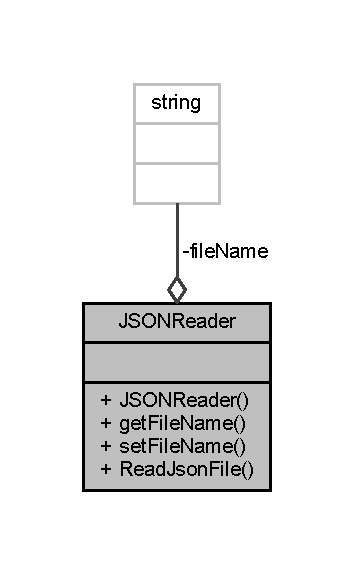
\includegraphics[width=170pt]{class_j_s_o_n_reader__coll__graph}
\end{center}
\end{figure}
\subsection*{Public Member Functions}
\begin{DoxyCompactItemize}
\item 
\hyperlink{class_j_s_o_n_reader_aa1480326d69874d2bab7183932b2d495}{J\+S\+O\+N\+Reader} (std\+::string f\+Name)
\item 
std\+::string \hyperlink{class_j_s_o_n_reader_abde6e34eccb5e195218923b8260391b2}{get\+File\+Name} ()
\item 
void \hyperlink{class_j_s_o_n_reader_ac9652f637597153cffe536fd2112c4f2}{set\+File\+Name} (std\+::string f\+Name)
\item 
std\+::ifstream \hyperlink{class_j_s_o_n_reader_a47c90ec12638eed9ea96feefc76096e1}{Read\+Json\+File} ()
\begin{DoxyCompactList}\small\item\em reads a J\+S\+ON file into the program \end{DoxyCompactList}\end{DoxyCompactItemize}
\subsection*{Private Attributes}
\begin{DoxyCompactItemize}
\item 
std\+::string \hyperlink{class_j_s_o_n_reader_abae0923ae887d87350b9ca1ddd56d41e}{file\+Name}
\end{DoxyCompactItemize}


\subsection{Detailed Description}
Reads in a J\+S\+ON file 

Definition at line 9 of file J\+S\+O\+N\+Reader.\+h.



\subsection{Constructor \& Destructor Documentation}
\mbox{\Hypertarget{class_j_s_o_n_reader_aa1480326d69874d2bab7183932b2d495}\label{class_j_s_o_n_reader_aa1480326d69874d2bab7183932b2d495}} 
\index{J\+S\+O\+N\+Reader@{J\+S\+O\+N\+Reader}!J\+S\+O\+N\+Reader@{J\+S\+O\+N\+Reader}}
\index{J\+S\+O\+N\+Reader@{J\+S\+O\+N\+Reader}!J\+S\+O\+N\+Reader@{J\+S\+O\+N\+Reader}}
\subsubsection{\texorpdfstring{J\+S\+O\+N\+Reader()}{JSONReader()}}
{\footnotesize\ttfamily J\+S\+O\+N\+Reader\+::\+J\+S\+O\+N\+Reader (\begin{DoxyParamCaption}\item[{std\+::string}]{f\+Name }\end{DoxyParamCaption})}



Definition at line 3 of file J\+S\+O\+N\+Reader.\+cpp.



References set\+File\+Name().


\begin{DoxyCode}
4 \{
5     \hyperlink{class_j_s_o_n_reader_ac9652f637597153cffe536fd2112c4f2}{setFileName}(fName);
6 \}
\end{DoxyCode}


\subsection{Member Function Documentation}
\mbox{\Hypertarget{class_j_s_o_n_reader_abde6e34eccb5e195218923b8260391b2}\label{class_j_s_o_n_reader_abde6e34eccb5e195218923b8260391b2}} 
\index{J\+S\+O\+N\+Reader@{J\+S\+O\+N\+Reader}!get\+File\+Name@{get\+File\+Name}}
\index{get\+File\+Name@{get\+File\+Name}!J\+S\+O\+N\+Reader@{J\+S\+O\+N\+Reader}}
\subsubsection{\texorpdfstring{get\+File\+Name()}{getFileName()}}
{\footnotesize\ttfamily std\+::string J\+S\+O\+N\+Reader\+::get\+File\+Name (\begin{DoxyParamCaption}{ }\end{DoxyParamCaption})}



Definition at line 8 of file J\+S\+O\+N\+Reader.\+cpp.



References file\+Name.


\begin{DoxyCode}
9 \{
10     \textcolor{keywordflow}{return} \hyperlink{class_j_s_o_n_reader_abae0923ae887d87350b9ca1ddd56d41e}{fileName};
11 \}
\end{DoxyCode}
\mbox{\Hypertarget{class_j_s_o_n_reader_a47c90ec12638eed9ea96feefc76096e1}\label{class_j_s_o_n_reader_a47c90ec12638eed9ea96feefc76096e1}} 
\index{J\+S\+O\+N\+Reader@{J\+S\+O\+N\+Reader}!Read\+Json\+File@{Read\+Json\+File}}
\index{Read\+Json\+File@{Read\+Json\+File}!J\+S\+O\+N\+Reader@{J\+S\+O\+N\+Reader}}
\subsubsection{\texorpdfstring{Read\+Json\+File()}{ReadJsonFile()}}
{\footnotesize\ttfamily std\+::ifstream J\+S\+O\+N\+Reader\+::\+Read\+Json\+File (\begin{DoxyParamCaption}{ }\end{DoxyParamCaption})}



reads a J\+S\+ON file into the program 



Definition at line 18 of file J\+S\+O\+N\+Reader.\+cpp.



References file\+Name.



Referenced by main().


\begin{DoxyCode}
19 \{
20     \textcolor{keywordflow}{return} std::ifstream(\hyperlink{class_j_s_o_n_reader_abae0923ae887d87350b9ca1ddd56d41e}{fileName}, std::ifstream::binary);
21 \}
\end{DoxyCode}
\mbox{\Hypertarget{class_j_s_o_n_reader_ac9652f637597153cffe536fd2112c4f2}\label{class_j_s_o_n_reader_ac9652f637597153cffe536fd2112c4f2}} 
\index{J\+S\+O\+N\+Reader@{J\+S\+O\+N\+Reader}!set\+File\+Name@{set\+File\+Name}}
\index{set\+File\+Name@{set\+File\+Name}!J\+S\+O\+N\+Reader@{J\+S\+O\+N\+Reader}}
\subsubsection{\texorpdfstring{set\+File\+Name()}{setFileName()}}
{\footnotesize\ttfamily void J\+S\+O\+N\+Reader\+::set\+File\+Name (\begin{DoxyParamCaption}\item[{std\+::string}]{f\+Name }\end{DoxyParamCaption})}



Definition at line 13 of file J\+S\+O\+N\+Reader.\+cpp.



References file\+Name.



Referenced by J\+S\+O\+N\+Reader().


\begin{DoxyCode}
14 \{
15     \hyperlink{class_j_s_o_n_reader_abae0923ae887d87350b9ca1ddd56d41e}{fileName} = fName;
16 \}
\end{DoxyCode}


\subsection{Member Data Documentation}
\mbox{\Hypertarget{class_j_s_o_n_reader_abae0923ae887d87350b9ca1ddd56d41e}\label{class_j_s_o_n_reader_abae0923ae887d87350b9ca1ddd56d41e}} 
\index{J\+S\+O\+N\+Reader@{J\+S\+O\+N\+Reader}!file\+Name@{file\+Name}}
\index{file\+Name@{file\+Name}!J\+S\+O\+N\+Reader@{J\+S\+O\+N\+Reader}}
\subsubsection{\texorpdfstring{file\+Name}{fileName}}
{\footnotesize\ttfamily std\+::string J\+S\+O\+N\+Reader\+::file\+Name\hspace{0.3cm}{\ttfamily [private]}}



Definition at line 21 of file J\+S\+O\+N\+Reader.\+h.



Referenced by get\+File\+Name(), Read\+Json\+File(), and set\+File\+Name().



The documentation for this class was generated from the following files\+:\begin{DoxyCompactItemize}
\item 
C\+:/\+Users/\+Kyle Tuckey/\+Documents/\+Final Year Project/\+Social\+\_\+\+N\+P\+C\+S/\+Social\+\_\+\+N\+P\+C\+S/\hyperlink{_j_s_o_n_reader_8h}{J\+S\+O\+N\+Reader.\+h}\item 
C\+:/\+Users/\+Kyle Tuckey/\+Documents/\+Final Year Project/\+Social\+\_\+\+N\+P\+C\+S/\+Social\+\_\+\+N\+P\+C\+S/\hyperlink{_j_s_o_n_reader_8cpp}{J\+S\+O\+N\+Reader.\+cpp}\end{DoxyCompactItemize}

\hypertarget{class_node}{}\section{Node Class Reference}
\label{class_node}\index{Node@{Node}}


{\ttfamily \#include $<$Node.\+h$>$}



Collaboration diagram for Node\+:\nopagebreak
\begin{figure}[H]
\begin{center}
\leavevmode
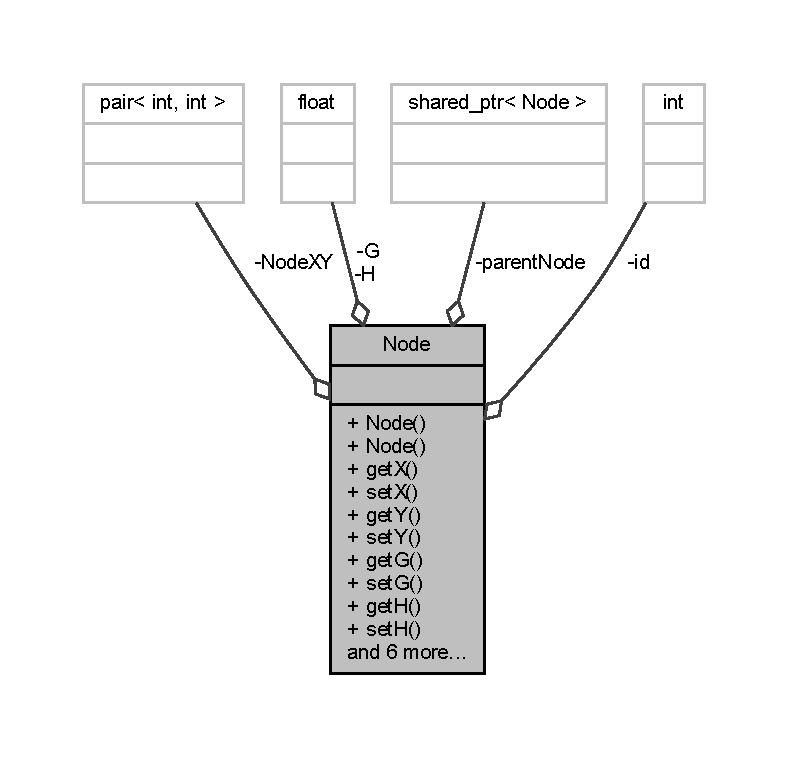
\includegraphics[width=350pt]{class_node__coll__graph}
\end{center}
\end{figure}
\subsection*{Public Member Functions}
\begin{DoxyCompactItemize}
\item 
\hyperlink{class_node_ad7a34779cad45d997bfd6d3d8043c75f}{Node} ()
\item 
\hyperlink{class_node_ad00949d1efbe6d24086446c2b16e8876}{Node} (int x, int y, std\+::shared\+\_\+ptr$<$ \hyperlink{class_node}{Node} $>$=nullptr)
\item 
int \hyperlink{class_node_a6c026e5d8c28591c6e2bd08c68619fd1}{getX} ()
\item 
void \hyperlink{class_node_adb106b3c9cca356ce404d45ce9ef1a89}{setX} (int x)
\item 
int \hyperlink{class_node_abab48a3f494994d4f456897f3372d3ae}{getY} ()
\item 
void \hyperlink{class_node_a2655bd886609cf39f486130733124ec7}{setY} (int y)
\item 
int \hyperlink{class_node_a9133c5c2e1c994b914535bbbefa33d7c}{getG} ()
\item 
void \hyperlink{class_node_acc878bf405f93ff15be94426b0f768f4}{setG} (int g)
\item 
int \hyperlink{class_node_a1108111505a673b217d5e13d6ac36d14}{getH} ()
\item 
void \hyperlink{class_node_a6076b0a2e7543341bd7b6e60c7635157}{setH} (int h)
\item 
int \hyperlink{class_node_a8dd9a1d6ac9638fd1168283ad47e5127}{get\+ID} ()
\item 
void \hyperlink{class_node_ae2ecbbfa7ede81db532c484e7e134fe6}{set\+ID} ()
\item 
std\+::shared\+\_\+ptr$<$ \hyperlink{class_node}{Node} $>$ \hyperlink{class_node_a5a7ffc7ca51647866a2d458cc8b42e00}{get\+Parent} ()
\item 
void \hyperlink{class_node_a5889e5c01190f75a7074e00c76f6a68a}{set\+Parent} (std\+::shared\+\_\+ptr$<$ \hyperlink{class_node}{Node} $>$ parent)
\item 
float \hyperlink{class_node_af483f2ed468aad829701a0ca7ba68966}{getF} ()
\item 
float \hyperlink{class_node_a2454f74ba33e81bd20945139c73e28fa}{man\+Hattan\+Distance} (std\+::shared\+\_\+ptr$<$ \hyperlink{class_node}{Node} $>$ node\+End)
\end{DoxyCompactItemize}
\subsection*{Private Attributes}
\begin{DoxyCompactItemize}
\item 
std\+::pair$<$ int, int $>$ \hyperlink{class_node_ac85b927d8c9cdc484f169129d317f6f0}{Node\+XY}
\item 
std\+::shared\+\_\+ptr$<$ \hyperlink{class_node}{Node} $>$ \hyperlink{class_node_aface6c6a7d38a7cc94090ef35bf9e95a}{parent\+Node}
\item 
int \hyperlink{class_node_a59a543130a10c95f1e8642cf8c5645e8}{id}
\item 
float \hyperlink{class_node_a3c6a67023068f762eaaa8a4861ab3e9f}{G}
\item 
float \hyperlink{class_node_a26426055f336a81dc05680b981e4c270}{H}
\end{DoxyCompactItemize}


\subsection{Detailed Description}


Definition at line 8 of file Node.\+h.



\subsection{Constructor \& Destructor Documentation}
\mbox{\Hypertarget{class_node_ad7a34779cad45d997bfd6d3d8043c75f}\label{class_node_ad7a34779cad45d997bfd6d3d8043c75f}} 
\index{Node@{Node}!Node@{Node}}
\index{Node@{Node}!Node@{Node}}
\subsubsection{\texorpdfstring{Node()}{Node()}\hspace{0.1cm}{\footnotesize\ttfamily [1/2]}}
{\footnotesize\ttfamily Node\+::\+Node (\begin{DoxyParamCaption}{ }\end{DoxyParamCaption})}



Definition at line 3 of file Node.\+cpp.


\begin{DoxyCode}
3 \{\}
\end{DoxyCode}
\mbox{\Hypertarget{class_node_ad00949d1efbe6d24086446c2b16e8876}\label{class_node_ad00949d1efbe6d24086446c2b16e8876}} 
\index{Node@{Node}!Node@{Node}}
\index{Node@{Node}!Node@{Node}}
\subsubsection{\texorpdfstring{Node()}{Node()}\hspace{0.1cm}{\footnotesize\ttfamily [2/2]}}
{\footnotesize\ttfamily Node\+::\+Node (\begin{DoxyParamCaption}\item[{int}]{x,  }\item[{int}]{y,  }\item[{std\+::shared\+\_\+ptr$<$ \hyperlink{class_node}{Node} $>$}]{node = {\ttfamily nullptr} }\end{DoxyParamCaption})}



Definition at line 5 of file Node.\+cpp.



References Node\+XY.


\begin{DoxyCode}
5                                                  : \hyperlink{class_node_a3c6a67023068f762eaaa8a4861ab3e9f}{G}(0), \hyperlink{class_node_a26426055f336a81dc05680b981e4c270}{H}(0)
6 \{
7     \hyperlink{class_node_ac85b927d8c9cdc484f169129d317f6f0}{NodeXY}.first = x;
8     \hyperlink{class_node_ac85b927d8c9cdc484f169129d317f6f0}{NodeXY}.second = y;
9 \}
\end{DoxyCode}


\subsection{Member Function Documentation}
\mbox{\Hypertarget{class_node_af483f2ed468aad829701a0ca7ba68966}\label{class_node_af483f2ed468aad829701a0ca7ba68966}} 
\index{Node@{Node}!getF@{getF}}
\index{getF@{getF}!Node@{Node}}
\subsubsection{\texorpdfstring{get\+F()}{getF()}}
{\footnotesize\ttfamily float Node\+::getF (\begin{DoxyParamCaption}{ }\end{DoxyParamCaption})}



Definition at line 31 of file Node.\+cpp.



References G, and H.


\begin{DoxyCode}
32 \{
33     \textcolor{keywordflow}{return} \hyperlink{class_node_a3c6a67023068f762eaaa8a4861ab3e9f}{G} + \hyperlink{class_node_a26426055f336a81dc05680b981e4c270}{H};
34 \}
\end{DoxyCode}
\mbox{\Hypertarget{class_node_a9133c5c2e1c994b914535bbbefa33d7c}\label{class_node_a9133c5c2e1c994b914535bbbefa33d7c}} 
\index{Node@{Node}!getG@{getG}}
\index{getG@{getG}!Node@{Node}}
\subsubsection{\texorpdfstring{get\+G()}{getG()}}
{\footnotesize\ttfamily int Node\+::getG (\begin{DoxyParamCaption}{ }\end{DoxyParamCaption})}

\mbox{\Hypertarget{class_node_a1108111505a673b217d5e13d6ac36d14}\label{class_node_a1108111505a673b217d5e13d6ac36d14}} 
\index{Node@{Node}!getH@{getH}}
\index{getH@{getH}!Node@{Node}}
\subsubsection{\texorpdfstring{get\+H()}{getH()}}
{\footnotesize\ttfamily int Node\+::getH (\begin{DoxyParamCaption}{ }\end{DoxyParamCaption})}

\mbox{\Hypertarget{class_node_a8dd9a1d6ac9638fd1168283ad47e5127}\label{class_node_a8dd9a1d6ac9638fd1168283ad47e5127}} 
\index{Node@{Node}!get\+ID@{get\+ID}}
\index{get\+ID@{get\+ID}!Node@{Node}}
\subsubsection{\texorpdfstring{get\+I\+D()}{getID()}}
{\footnotesize\ttfamily int Node\+::get\+ID (\begin{DoxyParamCaption}{ }\end{DoxyParamCaption})}

\mbox{\Hypertarget{class_node_a5a7ffc7ca51647866a2d458cc8b42e00}\label{class_node_a5a7ffc7ca51647866a2d458cc8b42e00}} 
\index{Node@{Node}!get\+Parent@{get\+Parent}}
\index{get\+Parent@{get\+Parent}!Node@{Node}}
\subsubsection{\texorpdfstring{get\+Parent()}{getParent()}}
{\footnotesize\ttfamily std\+::shared\+\_\+ptr$<$ \hyperlink{class_node}{Node} $>$ Node\+::get\+Parent (\begin{DoxyParamCaption}{ }\end{DoxyParamCaption})}



Definition at line 36 of file Node.\+cpp.



References parent\+Node.


\begin{DoxyCode}
37 \{
38     \textcolor{keywordflow}{return} \hyperlink{class_node_aface6c6a7d38a7cc94090ef35bf9e95a}{parentNode};
39 \}
\end{DoxyCode}
\mbox{\Hypertarget{class_node_a6c026e5d8c28591c6e2bd08c68619fd1}\label{class_node_a6c026e5d8c28591c6e2bd08c68619fd1}} 
\index{Node@{Node}!getX@{getX}}
\index{getX@{getX}!Node@{Node}}
\subsubsection{\texorpdfstring{get\+X()}{getX()}}
{\footnotesize\ttfamily int Node\+::getX (\begin{DoxyParamCaption}{ }\end{DoxyParamCaption})}



Definition at line 11 of file Node.\+cpp.



References Node\+XY.



Referenced by man\+Hattan\+Distance().


\begin{DoxyCode}
12 \{
13     \textcolor{keywordflow}{return} \hyperlink{class_node_ac85b927d8c9cdc484f169129d317f6f0}{NodeXY}.first;
14 \}
\end{DoxyCode}
\mbox{\Hypertarget{class_node_abab48a3f494994d4f456897f3372d3ae}\label{class_node_abab48a3f494994d4f456897f3372d3ae}} 
\index{Node@{Node}!getY@{getY}}
\index{getY@{getY}!Node@{Node}}
\subsubsection{\texorpdfstring{get\+Y()}{getY()}}
{\footnotesize\ttfamily int Node\+::getY (\begin{DoxyParamCaption}{ }\end{DoxyParamCaption})}



Definition at line 21 of file Node.\+cpp.



References Node\+XY.



Referenced by man\+Hattan\+Distance().


\begin{DoxyCode}
22 \{
23     \textcolor{keywordflow}{return} \hyperlink{class_node_ac85b927d8c9cdc484f169129d317f6f0}{NodeXY}.second;
24 \}
\end{DoxyCode}
\mbox{\Hypertarget{class_node_a2454f74ba33e81bd20945139c73e28fa}\label{class_node_a2454f74ba33e81bd20945139c73e28fa}} 
\index{Node@{Node}!man\+Hattan\+Distance@{man\+Hattan\+Distance}}
\index{man\+Hattan\+Distance@{man\+Hattan\+Distance}!Node@{Node}}
\subsubsection{\texorpdfstring{man\+Hattan\+Distance()}{manHattanDistance()}}
{\footnotesize\ttfamily float Node\+::man\+Hattan\+Distance (\begin{DoxyParamCaption}\item[{std\+::shared\+\_\+ptr$<$ \hyperlink{class_node}{Node} $>$}]{node\+End }\end{DoxyParamCaption})}



Definition at line 46 of file Node.\+cpp.



References get\+X(), and get\+Y().


\begin{DoxyCode}
47 \{
48     \textcolor{keywordtype}{float} x = (float)(fabs(this->\hyperlink{class_node_a6c026e5d8c28591c6e2bd08c68619fd1}{getX}() - endNode->getX()));
49     \textcolor{keywordtype}{float} y = (float)(fabs(this->\hyperlink{class_node_abab48a3f494994d4f456897f3372d3ae}{getY}() - endNode->getY()));
50 
51     \textcolor{keywordflow}{return} x + y;
52 \}
\end{DoxyCode}
\mbox{\Hypertarget{class_node_acc878bf405f93ff15be94426b0f768f4}\label{class_node_acc878bf405f93ff15be94426b0f768f4}} 
\index{Node@{Node}!setG@{setG}}
\index{setG@{setG}!Node@{Node}}
\subsubsection{\texorpdfstring{set\+G()}{setG()}}
{\footnotesize\ttfamily void Node\+::setG (\begin{DoxyParamCaption}\item[{int}]{g }\end{DoxyParamCaption})}

\mbox{\Hypertarget{class_node_a6076b0a2e7543341bd7b6e60c7635157}\label{class_node_a6076b0a2e7543341bd7b6e60c7635157}} 
\index{Node@{Node}!setH@{setH}}
\index{setH@{setH}!Node@{Node}}
\subsubsection{\texorpdfstring{set\+H()}{setH()}}
{\footnotesize\ttfamily void Node\+::setH (\begin{DoxyParamCaption}\item[{int}]{h }\end{DoxyParamCaption})}

\mbox{\Hypertarget{class_node_ae2ecbbfa7ede81db532c484e7e134fe6}\label{class_node_ae2ecbbfa7ede81db532c484e7e134fe6}} 
\index{Node@{Node}!set\+ID@{set\+ID}}
\index{set\+ID@{set\+ID}!Node@{Node}}
\subsubsection{\texorpdfstring{set\+I\+D()}{setID()}}
{\footnotesize\ttfamily void Node\+::set\+ID (\begin{DoxyParamCaption}{ }\end{DoxyParamCaption})}

\mbox{\Hypertarget{class_node_a5889e5c01190f75a7074e00c76f6a68a}\label{class_node_a5889e5c01190f75a7074e00c76f6a68a}} 
\index{Node@{Node}!set\+Parent@{set\+Parent}}
\index{set\+Parent@{set\+Parent}!Node@{Node}}
\subsubsection{\texorpdfstring{set\+Parent()}{setParent()}}
{\footnotesize\ttfamily void Node\+::set\+Parent (\begin{DoxyParamCaption}\item[{std\+::shared\+\_\+ptr$<$ \hyperlink{class_node}{Node} $>$}]{parent }\end{DoxyParamCaption})}



Definition at line 41 of file Node.\+cpp.



References parent\+Node.


\begin{DoxyCode}
42 \{
43     \hyperlink{class_node_aface6c6a7d38a7cc94090ef35bf9e95a}{parentNode} = nParent;
44 \}
\end{DoxyCode}
\mbox{\Hypertarget{class_node_adb106b3c9cca356ce404d45ce9ef1a89}\label{class_node_adb106b3c9cca356ce404d45ce9ef1a89}} 
\index{Node@{Node}!setX@{setX}}
\index{setX@{setX}!Node@{Node}}
\subsubsection{\texorpdfstring{set\+X()}{setX()}}
{\footnotesize\ttfamily void Node\+::setX (\begin{DoxyParamCaption}\item[{int}]{x }\end{DoxyParamCaption})}



Definition at line 16 of file Node.\+cpp.



References Node\+XY.


\begin{DoxyCode}
17 \{
18     \hyperlink{class_node_ac85b927d8c9cdc484f169129d317f6f0}{NodeXY}.first = nX;
19 \}
\end{DoxyCode}
\mbox{\Hypertarget{class_node_a2655bd886609cf39f486130733124ec7}\label{class_node_a2655bd886609cf39f486130733124ec7}} 
\index{Node@{Node}!setY@{setY}}
\index{setY@{setY}!Node@{Node}}
\subsubsection{\texorpdfstring{set\+Y()}{setY()}}
{\footnotesize\ttfamily void Node\+::setY (\begin{DoxyParamCaption}\item[{int}]{y }\end{DoxyParamCaption})}



Definition at line 26 of file Node.\+cpp.



References Node\+XY.


\begin{DoxyCode}
27 \{
28     \hyperlink{class_node_ac85b927d8c9cdc484f169129d317f6f0}{NodeXY}.second = nY;
29 \}
\end{DoxyCode}


\subsection{Member Data Documentation}
\mbox{\Hypertarget{class_node_a3c6a67023068f762eaaa8a4861ab3e9f}\label{class_node_a3c6a67023068f762eaaa8a4861ab3e9f}} 
\index{Node@{Node}!G@{G}}
\index{G@{G}!Node@{Node}}
\subsubsection{\texorpdfstring{G}{G}}
{\footnotesize\ttfamily float Node\+::G\hspace{0.3cm}{\ttfamily [private]}}



Definition at line 40 of file Node.\+h.



Referenced by get\+F().

\mbox{\Hypertarget{class_node_a26426055f336a81dc05680b981e4c270}\label{class_node_a26426055f336a81dc05680b981e4c270}} 
\index{Node@{Node}!H@{H}}
\index{H@{H}!Node@{Node}}
\subsubsection{\texorpdfstring{H}{H}}
{\footnotesize\ttfamily float Node\+::H\hspace{0.3cm}{\ttfamily [private]}}



Definition at line 41 of file Node.\+h.



Referenced by get\+F().

\mbox{\Hypertarget{class_node_a59a543130a10c95f1e8642cf8c5645e8}\label{class_node_a59a543130a10c95f1e8642cf8c5645e8}} 
\index{Node@{Node}!id@{id}}
\index{id@{id}!Node@{Node}}
\subsubsection{\texorpdfstring{id}{id}}
{\footnotesize\ttfamily int Node\+::id\hspace{0.3cm}{\ttfamily [private]}}



Definition at line 38 of file Node.\+h.

\mbox{\Hypertarget{class_node_ac85b927d8c9cdc484f169129d317f6f0}\label{class_node_ac85b927d8c9cdc484f169129d317f6f0}} 
\index{Node@{Node}!Node\+XY@{Node\+XY}}
\index{Node\+XY@{Node\+XY}!Node@{Node}}
\subsubsection{\texorpdfstring{Node\+XY}{NodeXY}}
{\footnotesize\ttfamily std\+::pair$<$int, int$>$ Node\+::\+Node\+XY\hspace{0.3cm}{\ttfamily [private]}}



Definition at line 35 of file Node.\+h.



Referenced by get\+X(), get\+Y(), Node(), set\+X(), and set\+Y().

\mbox{\Hypertarget{class_node_aface6c6a7d38a7cc94090ef35bf9e95a}\label{class_node_aface6c6a7d38a7cc94090ef35bf9e95a}} 
\index{Node@{Node}!parent\+Node@{parent\+Node}}
\index{parent\+Node@{parent\+Node}!Node@{Node}}
\subsubsection{\texorpdfstring{parent\+Node}{parentNode}}
{\footnotesize\ttfamily std\+::shared\+\_\+ptr$<$\hyperlink{class_node}{Node}$>$ Node\+::parent\+Node\hspace{0.3cm}{\ttfamily [private]}}



Definition at line 36 of file Node.\+h.



Referenced by get\+Parent(), and set\+Parent().



The documentation for this class was generated from the following files\+:\begin{DoxyCompactItemize}
\item 
C\+:/\+Users/\+Kyle Tuckey/\+Documents/\+Final Year Project/\+Social\+\_\+\+N\+P\+C\+S/\+Social\+\_\+\+N\+P\+C\+S/\hyperlink{_node_8h}{Node.\+h}\item 
C\+:/\+Users/\+Kyle Tuckey/\+Documents/\+Final Year Project/\+Social\+\_\+\+N\+P\+C\+S/\+Social\+\_\+\+N\+P\+C\+S/\hyperlink{_node_8cpp}{Node.\+cpp}\end{DoxyCompactItemize}

\hypertarget{class_n_p_c}{}\section{N\+PC Class Reference}
\label{class_n_p_c}\index{N\+PC@{N\+PC}}


{\ttfamily \#include $<$N\+P\+C.\+h$>$}



Inheritance diagram for N\+PC\+:\nopagebreak
\begin{figure}[H]
\begin{center}
\leavevmode
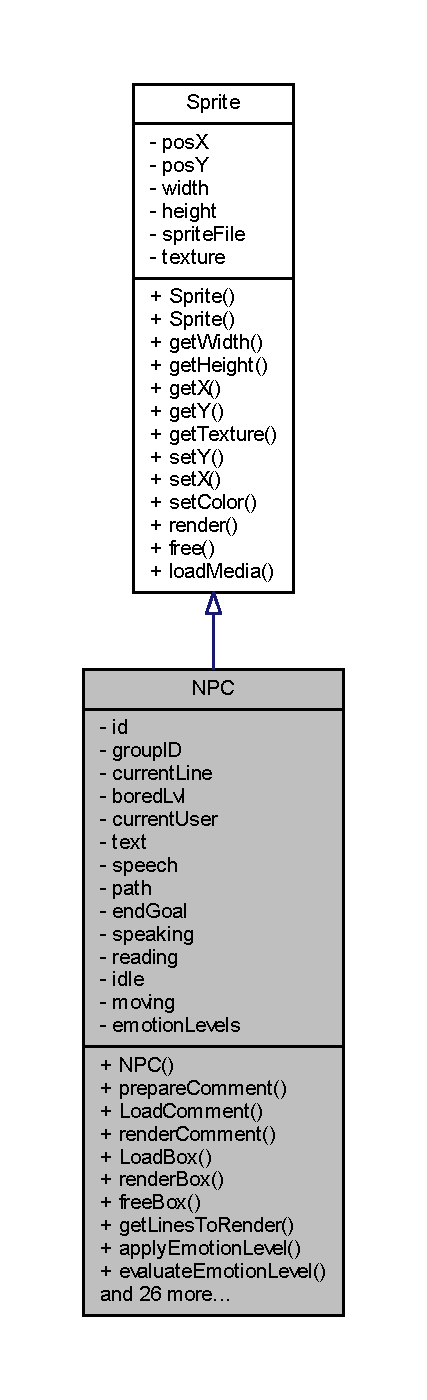
\includegraphics[height=550pt]{class_n_p_c__inherit__graph}
\end{center}
\end{figure}


Collaboration diagram for N\+PC\+:\nopagebreak
\begin{figure}[H]
\begin{center}
\leavevmode
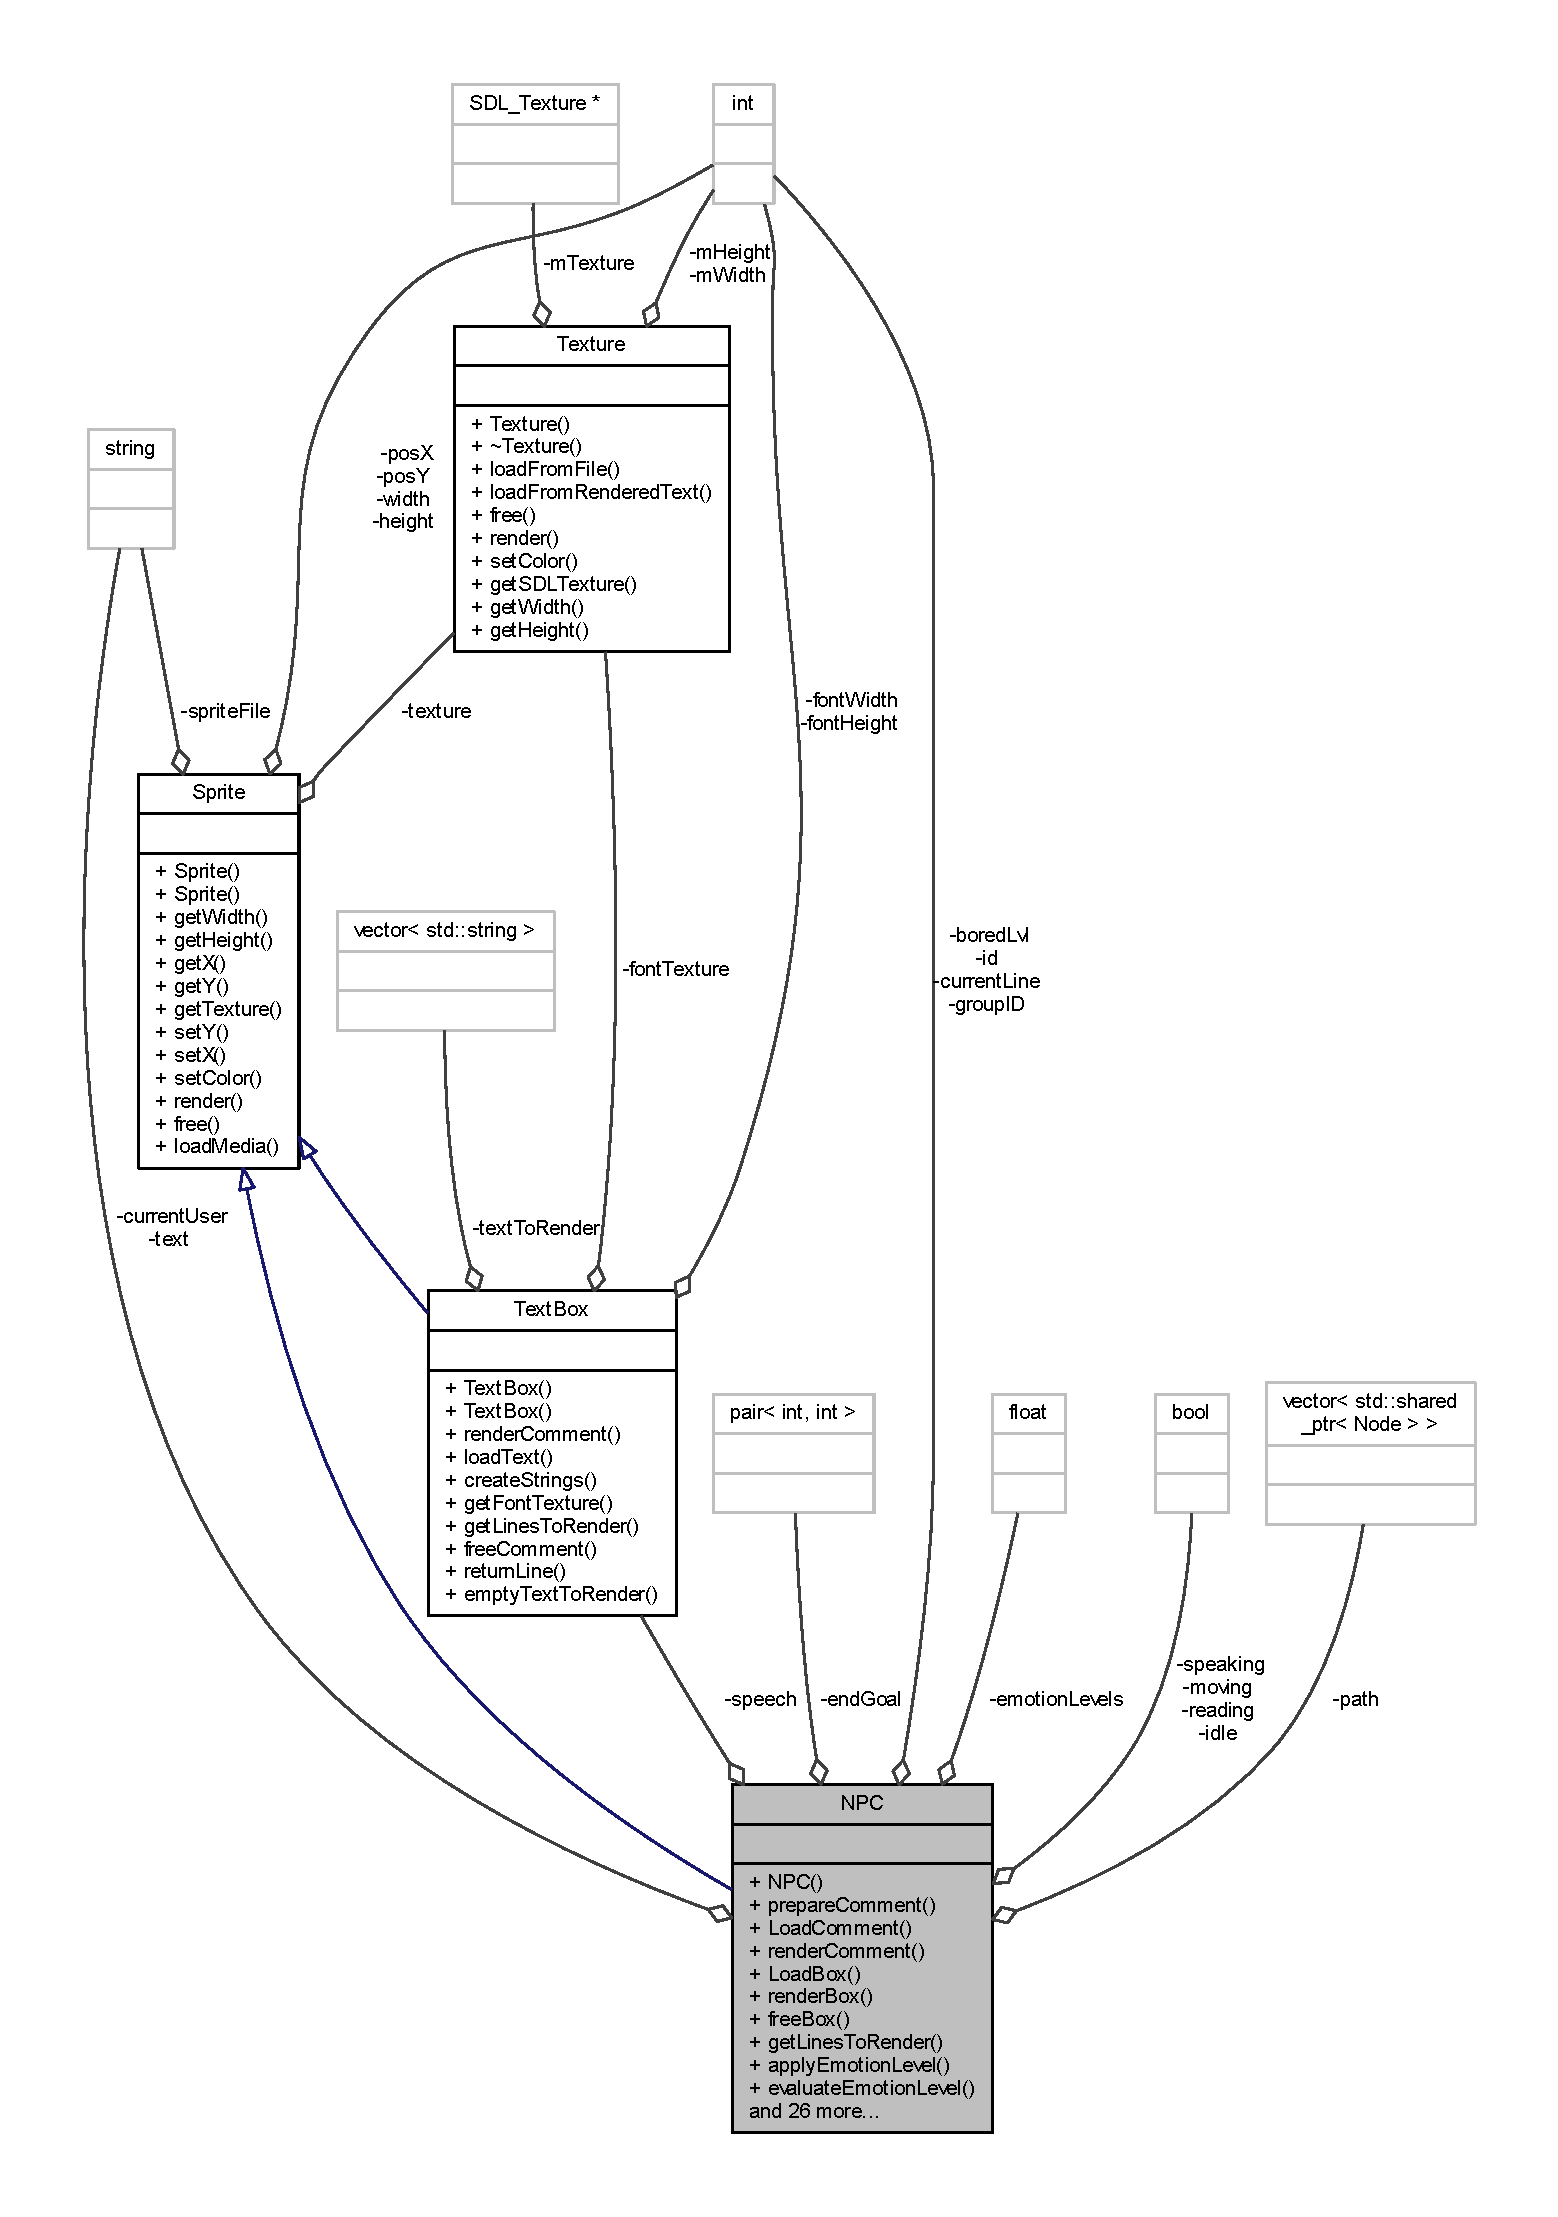
\includegraphics[width=350pt]{class_n_p_c__coll__graph}
\end{center}
\end{figure}
\subsection*{Public Member Functions}
\begin{DoxyCompactItemize}
\item 
\hyperlink{class_n_p_c_a9db0a86ef6a5ab2b406c46c8ec6d740a}{N\+PC} (std\+::string t\+Box\+Sprite, std\+::string N\+P\+C\+Sprite, std\+::string \hyperlink{class_n_p_c_a64ad332dcfeb84a7a6bedd404378f05b}{text}, S\+D\+L\+\_\+\+Renderer $\ast$renderer, int x, int y)
\item 
void \hyperlink{class_n_p_c_af0a849c937b7d765b2bec4d122a2b62c}{prepare\+Comment} (std\+::string txt, T\+T\+F\+\_\+\+Font $\ast$font)
\begin{DoxyCompactList}\small\item\em Breaks up parsed in text into a chunked comment. \end{DoxyCompactList}\item 
void \hyperlink{class_n_p_c_a468647f008c7e65f2a25be9dcd5e5968}{Load\+Comment} (S\+D\+L\+\_\+\+Renderer $\ast$renderer, int i, T\+T\+F\+\_\+\+Font $\ast$font)
\begin{DoxyCompactList}\small\item\em Loads the N\+P\+Cs comment into the textbox. \end{DoxyCompactList}\item 
void \hyperlink{class_n_p_c_abfad5a818584b5ee6fab0605873ae5c4}{render\+Comment} (S\+D\+L\+\_\+\+Renderer $\ast$renderer)
\begin{DoxyCompactList}\small\item\em Renders the N\+P\+Cs comment. \end{DoxyCompactList}\item 
void \hyperlink{class_n_p_c_aa9d97773d1a9b49e2a8dd5adaa23beff}{Load\+Box} (S\+D\+L\+\_\+\+Renderer $\ast$renderer)
\begin{DoxyCompactList}\small\item\em Loads the N\+P\+Cs \hyperlink{class_text_box}{Text\+Box}. \end{DoxyCompactList}\item 
void \hyperlink{class_n_p_c_ad5e9a664ceae6a920e63d34f2738b21d}{render\+Box} (S\+D\+L\+\_\+\+Renderer $\ast$renderer)
\begin{DoxyCompactList}\small\item\em Renders the N\+P\+Cs \hyperlink{class_text_box}{Text\+Box}. \end{DoxyCompactList}\item 
void \hyperlink{class_n_p_c_abacec0f0add55305f86ad56e4c80cd18}{free\+Box} ()
\begin{DoxyCompactList}\small\item\em Frees up the memory space the textbox is occupying. \end{DoxyCompactList}\item 
int \hyperlink{class_n_p_c_a64425a9a6a4b6262e4f9e0a4e5169ce4}{get\+Lines\+To\+Render} ()
\begin{DoxyCompactList}\small\item\em returns the number of line being rendered to the screen \end{DoxyCompactList}\item 
void \hyperlink{class_n_p_c_a3cb8421a139170f47247b1e126eb722b}{apply\+Emotion\+Level} (float polarity)
\item 
void \hyperlink{class_n_p_c_a278f18152374a82602f57f98c0a43800}{evaluate\+Emotion\+Level} ()
\begin{DoxyCompactList}\small\item\em Evaluates the emotional level of the \hyperlink{class_n_p_c}{N\+PC}. \end{DoxyCompactList}\item 
void \hyperlink{class_n_p_c_abaa15a4fd5a37a62983d7fd2acafe271}{move} ()
\begin{DoxyCompactList}\small\item\em Handles the N\+P\+Cs movement. \end{DoxyCompactList}\item 
void \hyperlink{class_n_p_c_a81d67fe2002ad57334c40fadcba25dc4}{set\+ID} (int i)
\item 
int \hyperlink{class_n_p_c_ac4588139be32c307a0d31e302f377dea}{get\+ID} ()
\item 
int \hyperlink{class_n_p_c_a7ea10930901666fc087de1a74d339b84}{get\+Group\+ID} ()
\item 
void \hyperlink{class_n_p_c_aaa89e6f11f1bda185769ae321f345960}{set\+Group\+ID} (int \hyperlink{class_n_p_c_a1b705223f885df652f2faffc4735d03c}{id})
\item 
int \hyperlink{class_n_p_c_a83d65db3ffe79025091a655d92fe4f27}{get\+Current\+Line} ()
\item 
void \hyperlink{class_n_p_c_ac2143e6bbc303d3fbe65c5603746557e}{set\+Current\+Line} (int \hyperlink{class_n_p_c_a1b705223f885df652f2faffc4735d03c}{id})
\item 
bool \hyperlink{class_n_p_c_a759c42c8f2a75d2684157574cf3ddc65}{get\+Speaking} ()
\item 
void \hyperlink{class_n_p_c_a16d67a6d98c54df2fe320c64c5680285}{set\+Speaking} (bool val)
\item 
float \hyperlink{class_n_p_c_a6ee0944f7b8cdf1ab5ab164b3d7074bc}{get\+Emotion\+Level} ()
\item 
bool \hyperlink{class_n_p_c_a5f19b3b029fd8366921b5bb71335ee9a}{get\+Idle} ()
\item 
void \hyperlink{class_n_p_c_a154d9c6f7c920edcfaeb20f826419ac6}{set\+Idle} (bool n\+Idle)
\item 
bool \hyperlink{class_n_p_c_acb2a20f35f7bb54569032cc1b6a67be0}{get\+Moving} ()
\item 
void \hyperlink{class_n_p_c_af18588e2baa382f12e4e9fe56fc247bc}{set\+Moving} (bool \hyperlink{class_n_p_c_abaa15a4fd5a37a62983d7fd2acafe271}{move})
\item 
bool \hyperlink{class_n_p_c_a723183afdc657db3ec2ef88779e80968}{get\+Reading} ()
\item 
void \hyperlink{class_n_p_c_a9e0ab46138990129c16b78c2a6ee6e25}{set\+Reading} (bool read)
\item 
int \hyperlink{class_n_p_c_a6e50d697a2444e3aff5bfce6252f7bb5}{get\+Boredom} ()
\item 
void \hyperlink{class_n_p_c_a3e24b9fe9d34b635c2f57c48eab0b29d}{set\+Boredom} (int lvl)
\item 
std\+::string \hyperlink{class_n_p_c_a289f4c34cf597a7e61f787844f80a356}{get\+Current\+User} ()
\item 
void \hyperlink{class_n_p_c_a30076f45e31741e86a79f280eca215cb}{set\+Current\+User} (std\+::string user)
\item 
std\+::vector$<$ std\+::shared\+\_\+ptr$<$ \hyperlink{class_node}{Node} $>$ $>$ \hyperlink{class_n_p_c_aa9a219c85034a65f903f38781356b05b}{get\+Path} ()
\item 
void \hyperlink{class_n_p_c_a9582ddb2cc78ad77c8ded77e192be5b0}{set\+Path} (std\+::vector$<$ std\+::shared\+\_\+ptr$<$ \hyperlink{class_node}{Node} $>$$>$ new\+Path)
\item 
std\+::string \hyperlink{class_n_p_c_a480c5ef808977d9d81aef0f9e7b2093f}{get\+Text} ()
\item 
void \hyperlink{class_n_p_c_ae94160d4a1fe8d5195e9ae66f78059ce}{set\+Text} (std\+::string t)
\item 
std\+::pair$<$ int, int $>$ \hyperlink{class_n_p_c_a64a6c85370defc9094cf5e597a7bc85d}{get\+End\+Goal} ()
\item 
void \hyperlink{class_n_p_c_aefc13625a35497cf6158c15692c52eda}{set\+End\+Goal} (std\+::pair$<$ int, int $>$ new\+Goal)
\end{DoxyCompactItemize}
\subsection*{Private Attributes}
\begin{DoxyCompactItemize}
\item 
int \hyperlink{class_n_p_c_a1b705223f885df652f2faffc4735d03c}{id}
\item 
int \hyperlink{class_n_p_c_ab370e8a4fbb5ccabdc06821f7dfda428}{group\+ID}
\item 
int \hyperlink{class_n_p_c_a0969e4514a21f3b2966a24d78e9e3343}{current\+Line}
\item 
int \hyperlink{class_n_p_c_a1f67b7dfca770653fc523dfc558e7fdf}{bored\+Lvl}
\item 
std\+::string \hyperlink{class_n_p_c_a944f970943002adc4f0c970b0200c011}{current\+User} = \char`\"{}\char`\"{}
\item 
std\+::string \hyperlink{class_n_p_c_a64ad332dcfeb84a7a6bedd404378f05b}{text}
\item 
\hyperlink{class_text_box}{Text\+Box} \hyperlink{class_n_p_c_a1a1be15df827227f45559388897a9cd5}{speech}
\item 
std\+::vector$<$ std\+::shared\+\_\+ptr$<$ \hyperlink{class_node}{Node} $>$ $>$ \hyperlink{class_n_p_c_afdd6b1a6e4827259ec9d9fcd075cb099}{path}
\item 
std\+::pair$<$ int, int $>$ \hyperlink{class_n_p_c_ab2349a8d6757b61a73f87de9cba387d1}{end\+Goal}
\item 
bool \hyperlink{class_n_p_c_a0dc17cd2d9b7d486e6d74089819117e7}{speaking} = false
\item 
bool \hyperlink{class_n_p_c_a04d8f196cdd6de84f38131836d9c9cc7}{reading} = false
\item 
bool \hyperlink{class_n_p_c_aa228d3e449507a6326cef7b449752e62}{idle} = false
\item 
bool \hyperlink{class_n_p_c_a4dfc6a89cae1301e7f722bbba67f3dbb}{moving} = false
\item 
float \hyperlink{class_n_p_c_a804b5c812457417231e3b4ab5e06ac88}{emotion\+Levels} = 0.\+0f
\end{DoxyCompactItemize}
\subsection*{Friends}
\begin{DoxyCompactItemize}
\item 
bool \hyperlink{class_n_p_c_a3e1f9defd10ab4be568a190fbcd0ac07}{operator==} (const \hyperlink{class_n_p_c}{N\+PC} \&c1, const \hyperlink{class_n_p_c}{N\+PC} \&c2)
\end{DoxyCompactItemize}


\subsection{Detailed Description}
\hyperlink{class_n_p_c}{N\+PC} class inherits from sprite class, uses the textbox class in conjunction with it\textquotesingle{}s base rendering methods for the \hyperlink{class_n_p_c}{N\+PC} sprite. holds all the actions a \hyperlink{class_n_p_c}{N\+PC} can perform within the application. 

Definition at line 9 of file N\+P\+C.\+h.



\subsection{Constructor \& Destructor Documentation}
\mbox{\Hypertarget{class_n_p_c_a9db0a86ef6a5ab2b406c46c8ec6d740a}\label{class_n_p_c_a9db0a86ef6a5ab2b406c46c8ec6d740a}} 
\index{N\+PC@{N\+PC}!N\+PC@{N\+PC}}
\index{N\+PC@{N\+PC}!N\+PC@{N\+PC}}
\subsubsection{\texorpdfstring{N\+P\+C()}{NPC()}}
{\footnotesize\ttfamily N\+P\+C\+::\+N\+PC (\begin{DoxyParamCaption}\item[{std\+::string}]{t\+Box\+Sprite,  }\item[{std\+::string}]{N\+P\+C\+Sprite,  }\item[{std\+::string}]{text,  }\item[{S\+D\+L\+\_\+\+Renderer $\ast$}]{renderer,  }\item[{int}]{x,  }\item[{int}]{y }\end{DoxyParamCaption})}



Definition at line 3 of file N\+P\+C.\+cpp.



References bored\+Lvl, and speech.


\begin{DoxyCode}
3                                                                                                         : 
      \hyperlink{class_sprite_a12cba3ac1868418add3c4d95ce87e615}{Sprite}(NPCSprite, renderer, x, y)
4 \{
5     \hyperlink{class_n_p_c_a1f67b7dfca770653fc523dfc558e7fdf}{boredLvl} = 0;
6     \hyperlink{class_n_p_c_a1a1be15df827227f45559388897a9cd5}{speech} = \hyperlink{class_text_box}{TextBox}(tBoxSprite, renderer, x, y);
7 \}
\end{DoxyCode}


\subsection{Member Function Documentation}
\mbox{\Hypertarget{class_n_p_c_a3cb8421a139170f47247b1e126eb722b}\label{class_n_p_c_a3cb8421a139170f47247b1e126eb722b}} 
\index{N\+PC@{N\+PC}!apply\+Emotion\+Level@{apply\+Emotion\+Level}}
\index{apply\+Emotion\+Level@{apply\+Emotion\+Level}!N\+PC@{N\+PC}}
\subsubsection{\texorpdfstring{apply\+Emotion\+Level()}{applyEmotionLevel()}}
{\footnotesize\ttfamily void N\+P\+C\+::apply\+Emotion\+Level (\begin{DoxyParamCaption}\item[{float}]{polarity }\end{DoxyParamCaption})}



Definition at line 200 of file N\+P\+C.\+cpp.



References emotion\+Levels.


\begin{DoxyCode}
201 \{
202     \hyperlink{class_n_p_c_a804b5c812457417231e3b4ab5e06ac88}{emotionLevels} += val;
203 \}
\end{DoxyCode}
\mbox{\Hypertarget{class_n_p_c_a278f18152374a82602f57f98c0a43800}\label{class_n_p_c_a278f18152374a82602f57f98c0a43800}} 
\index{N\+PC@{N\+PC}!evaluate\+Emotion\+Level@{evaluate\+Emotion\+Level}}
\index{evaluate\+Emotion\+Level@{evaluate\+Emotion\+Level}!N\+PC@{N\+PC}}
\subsubsection{\texorpdfstring{evaluate\+Emotion\+Level()}{evaluateEmotionLevel()}}
{\footnotesize\ttfamily void N\+P\+C\+::evaluate\+Emotion\+Level (\begin{DoxyParamCaption}{ }\end{DoxyParamCaption})}



Evaluates the emotional level of the \hyperlink{class_n_p_c}{N\+PC}. 

Evaluates the N\+P\+Cs emotion level and converts it into R\+GB values 

Definition at line 157 of file N\+P\+C.\+cpp.



References get\+Emotion\+Level(), and Sprite\+::set\+Color().


\begin{DoxyCode}
158 \{
159     \textcolor{keywordtype}{int} emo = \hyperlink{class_n_p_c_a6ee0944f7b8cdf1ab5ab164b3d7074bc}{getEmotionLevel}();
160 
161     \textcolor{comment}{// if the emotion level is less than 0 it is negative}
162     \textcolor{keywordflow}{if} (emo < 0)
163     \{
164         emo = abs(emo) * 10;
165 
166         \textcolor{comment}{// ensure that the highest possible value is 255}
167         \textcolor{keywordflow}{if} (emo > 255)
168             emo = 255;
169 
170         \textcolor{comment}{// set the NPCs color to be more red to show negativity}
171         \hyperlink{class_sprite_a1ca0939610f24386a4eecb8e91688c65}{setColor}(255, 255-emo, 255-emo);
172     \}
173     \textcolor{keywordflow}{else} \textcolor{keywordflow}{if}(emo > 0)
174     \{
175 
176         emo = emo * 10;
177 
178         \textcolor{keywordflow}{if} (emo > 255)
179             emo = 255;
180 
181         \textcolor{comment}{// set the NPCs color to be more green to show positivity}
182         \hyperlink{class_sprite_a1ca0939610f24386a4eecb8e91688c65}{setColor}(255-emo, 255, 255-emo);
183     \}
184 \}
\end{DoxyCode}
\mbox{\Hypertarget{class_n_p_c_abacec0f0add55305f86ad56e4c80cd18}\label{class_n_p_c_abacec0f0add55305f86ad56e4c80cd18}} 
\index{N\+PC@{N\+PC}!free\+Box@{free\+Box}}
\index{free\+Box@{free\+Box}!N\+PC@{N\+PC}}
\subsubsection{\texorpdfstring{free\+Box()}{freeBox()}}
{\footnotesize\ttfamily void N\+P\+C\+::free\+Box (\begin{DoxyParamCaption}{ }\end{DoxyParamCaption})}



Frees up the memory space the textbox is occupying. 

Frees the space that both the comment and its textbox occupy in memory 

Definition at line 128 of file N\+P\+C.\+cpp.



References Sprite\+::free(), Text\+Box\+::free\+Comment(), and speech.


\begin{DoxyCode}
129 \{
130     \hyperlink{class_n_p_c_a1a1be15df827227f45559388897a9cd5}{speech}.\hyperlink{class_sprite_abce3359b4f055bac7384038046ed9ead}{free}();
131     \hyperlink{class_n_p_c_a1a1be15df827227f45559388897a9cd5}{speech}.\hyperlink{class_text_box_a6ab09c23671be63b41bd0eba32d385e3}{freeComment}();
132 \}
\end{DoxyCode}
\mbox{\Hypertarget{class_n_p_c_a6e50d697a2444e3aff5bfce6252f7bb5}\label{class_n_p_c_a6e50d697a2444e3aff5bfce6252f7bb5}} 
\index{N\+PC@{N\+PC}!get\+Boredom@{get\+Boredom}}
\index{get\+Boredom@{get\+Boredom}!N\+PC@{N\+PC}}
\subsubsection{\texorpdfstring{get\+Boredom()}{getBoredom()}}
{\footnotesize\ttfamily int N\+P\+C\+::get\+Boredom (\begin{DoxyParamCaption}{ }\end{DoxyParamCaption})}



Definition at line 47 of file N\+P\+C.\+cpp.



References bored\+Lvl.


\begin{DoxyCode}
48 \{
49     \textcolor{keywordflow}{return} \hyperlink{class_n_p_c_a1f67b7dfca770653fc523dfc558e7fdf}{boredLvl};
50 \}
\end{DoxyCode}
\mbox{\Hypertarget{class_n_p_c_a83d65db3ffe79025091a655d92fe4f27}\label{class_n_p_c_a83d65db3ffe79025091a655d92fe4f27}} 
\index{N\+PC@{N\+PC}!get\+Current\+Line@{get\+Current\+Line}}
\index{get\+Current\+Line@{get\+Current\+Line}!N\+PC@{N\+PC}}
\subsubsection{\texorpdfstring{get\+Current\+Line()}{getCurrentLine()}}
{\footnotesize\ttfamily int N\+P\+C\+::get\+Current\+Line (\begin{DoxyParamCaption}{ }\end{DoxyParamCaption})}



Definition at line 185 of file N\+P\+C.\+cpp.



References current\+Line.


\begin{DoxyCode}
186 \{
187     \textcolor{keywordflow}{return} \hyperlink{class_n_p_c_a0969e4514a21f3b2966a24d78e9e3343}{currentLine};
188 \}
\end{DoxyCode}
\mbox{\Hypertarget{class_n_p_c_a289f4c34cf597a7e61f787844f80a356}\label{class_n_p_c_a289f4c34cf597a7e61f787844f80a356}} 
\index{N\+PC@{N\+PC}!get\+Current\+User@{get\+Current\+User}}
\index{get\+Current\+User@{get\+Current\+User}!N\+PC@{N\+PC}}
\subsubsection{\texorpdfstring{get\+Current\+User()}{getCurrentUser()}}
{\footnotesize\ttfamily std\+::string N\+P\+C\+::get\+Current\+User (\begin{DoxyParamCaption}{ }\end{DoxyParamCaption})}



Definition at line 52 of file N\+P\+C.\+cpp.



References current\+User.


\begin{DoxyCode}
53 \{
54     \textcolor{keywordflow}{return} \hyperlink{class_n_p_c_a944f970943002adc4f0c970b0200c011}{currentUser};
55 \}
\end{DoxyCode}
\mbox{\Hypertarget{class_n_p_c_a6ee0944f7b8cdf1ab5ab164b3d7074bc}\label{class_n_p_c_a6ee0944f7b8cdf1ab5ab164b3d7074bc}} 
\index{N\+PC@{N\+PC}!get\+Emotion\+Level@{get\+Emotion\+Level}}
\index{get\+Emotion\+Level@{get\+Emotion\+Level}!N\+PC@{N\+PC}}
\subsubsection{\texorpdfstring{get\+Emotion\+Level()}{getEmotionLevel()}}
{\footnotesize\ttfamily float N\+P\+C\+::get\+Emotion\+Level (\begin{DoxyParamCaption}{ }\end{DoxyParamCaption})}



Definition at line 149 of file N\+P\+C.\+cpp.



References emotion\+Levels.



Referenced by evaluate\+Emotion\+Level().


\begin{DoxyCode}
150 \{
151     \textcolor{keywordflow}{return} \hyperlink{class_n_p_c_a804b5c812457417231e3b4ab5e06ac88}{emotionLevels};
152 \}
\end{DoxyCode}
\mbox{\Hypertarget{class_n_p_c_a64a6c85370defc9094cf5e597a7bc85d}\label{class_n_p_c_a64a6c85370defc9094cf5e597a7bc85d}} 
\index{N\+PC@{N\+PC}!get\+End\+Goal@{get\+End\+Goal}}
\index{get\+End\+Goal@{get\+End\+Goal}!N\+PC@{N\+PC}}
\subsubsection{\texorpdfstring{get\+End\+Goal()}{getEndGoal()}}
{\footnotesize\ttfamily std\+::pair$<$ int, int $>$ N\+P\+C\+::get\+End\+Goal (\begin{DoxyParamCaption}{ }\end{DoxyParamCaption})}



Definition at line 225 of file N\+P\+C.\+cpp.



References end\+Goal.


\begin{DoxyCode}
226 \{
227     \textcolor{keywordflow}{return} \hyperlink{class_n_p_c_ab2349a8d6757b61a73f87de9cba387d1}{endGoal};
228 \}
\end{DoxyCode}
\mbox{\Hypertarget{class_n_p_c_a7ea10930901666fc087de1a74d339b84}\label{class_n_p_c_a7ea10930901666fc087de1a74d339b84}} 
\index{N\+PC@{N\+PC}!get\+Group\+ID@{get\+Group\+ID}}
\index{get\+Group\+ID@{get\+Group\+ID}!N\+PC@{N\+PC}}
\subsubsection{\texorpdfstring{get\+Group\+I\+D()}{getGroupID()}}
{\footnotesize\ttfamily int N\+P\+C\+::get\+Group\+ID (\begin{DoxyParamCaption}{ }\end{DoxyParamCaption})}



Definition at line 42 of file N\+P\+C.\+cpp.



References group\+ID.


\begin{DoxyCode}
43 \{
44     \textcolor{keywordflow}{return} \hyperlink{class_n_p_c_ab370e8a4fbb5ccabdc06821f7dfda428}{groupID};
45 \}
\end{DoxyCode}
\mbox{\Hypertarget{class_n_p_c_ac4588139be32c307a0d31e302f377dea}\label{class_n_p_c_ac4588139be32c307a0d31e302f377dea}} 
\index{N\+PC@{N\+PC}!get\+ID@{get\+ID}}
\index{get\+ID@{get\+ID}!N\+PC@{N\+PC}}
\subsubsection{\texorpdfstring{get\+I\+D()}{getID()}}
{\footnotesize\ttfamily int N\+P\+C\+::get\+ID (\begin{DoxyParamCaption}{ }\end{DoxyParamCaption})}



Definition at line 32 of file N\+P\+C.\+cpp.



References id.


\begin{DoxyCode}
33 \{
34     \textcolor{keywordflow}{return} \hyperlink{class_n_p_c_a1b705223f885df652f2faffc4735d03c}{id};
35 \}
\end{DoxyCode}
\mbox{\Hypertarget{class_n_p_c_a5f19b3b029fd8366921b5bb71335ee9a}\label{class_n_p_c_a5f19b3b029fd8366921b5bb71335ee9a}} 
\index{N\+PC@{N\+PC}!get\+Idle@{get\+Idle}}
\index{get\+Idle@{get\+Idle}!N\+PC@{N\+PC}}
\subsubsection{\texorpdfstring{get\+Idle()}{getIdle()}}
{\footnotesize\ttfamily bool N\+P\+C\+::get\+Idle (\begin{DoxyParamCaption}{ }\end{DoxyParamCaption})}



Definition at line 215 of file N\+P\+C.\+cpp.



References idle.


\begin{DoxyCode}
216 \{
217     \textcolor{keywordflow}{return} \hyperlink{class_n_p_c_aa228d3e449507a6326cef7b449752e62}{idle};
218 \}
\end{DoxyCode}
\mbox{\Hypertarget{class_n_p_c_a64425a9a6a4b6262e4f9e0a4e5169ce4}\label{class_n_p_c_a64425a9a6a4b6262e4f9e0a4e5169ce4}} 
\index{N\+PC@{N\+PC}!get\+Lines\+To\+Render@{get\+Lines\+To\+Render}}
\index{get\+Lines\+To\+Render@{get\+Lines\+To\+Render}!N\+PC@{N\+PC}}
\subsubsection{\texorpdfstring{get\+Lines\+To\+Render()}{getLinesToRender()}}
{\footnotesize\ttfamily int N\+P\+C\+::get\+Lines\+To\+Render (\begin{DoxyParamCaption}{ }\end{DoxyParamCaption})}



returns the number of line being rendered to the screen 



Definition at line 139 of file N\+P\+C.\+cpp.



References Text\+Box\+::get\+Lines\+To\+Render(), and speech.


\begin{DoxyCode}
140 \{
141     \textcolor{keywordflow}{return} \hyperlink{class_n_p_c_a1a1be15df827227f45559388897a9cd5}{speech}.\hyperlink{class_text_box_a7c620113713b6b841ef7e183c1d81312}{getLinesToRender}();
142 \}
\end{DoxyCode}
\mbox{\Hypertarget{class_n_p_c_acb2a20f35f7bb54569032cc1b6a67be0}\label{class_n_p_c_acb2a20f35f7bb54569032cc1b6a67be0}} 
\index{N\+PC@{N\+PC}!get\+Moving@{get\+Moving}}
\index{get\+Moving@{get\+Moving}!N\+PC@{N\+PC}}
\subsubsection{\texorpdfstring{get\+Moving()}{getMoving()}}
{\footnotesize\ttfamily bool N\+P\+C\+::get\+Moving (\begin{DoxyParamCaption}{ }\end{DoxyParamCaption})}



Definition at line 254 of file N\+P\+C.\+cpp.



References moving.


\begin{DoxyCode}
255 \{
256     \textcolor{keywordflow}{return} \hyperlink{class_n_p_c_a4dfc6a89cae1301e7f722bbba67f3dbb}{moving};
257 \}
\end{DoxyCode}
\mbox{\Hypertarget{class_n_p_c_aa9a219c85034a65f903f38781356b05b}\label{class_n_p_c_aa9a219c85034a65f903f38781356b05b}} 
\index{N\+PC@{N\+PC}!get\+Path@{get\+Path}}
\index{get\+Path@{get\+Path}!N\+PC@{N\+PC}}
\subsubsection{\texorpdfstring{get\+Path()}{getPath()}}
{\footnotesize\ttfamily std\+::vector$<$ std\+::shared\+\_\+ptr$<$ \hyperlink{class_node}{Node} $>$ $>$ N\+P\+C\+::get\+Path (\begin{DoxyParamCaption}{ }\end{DoxyParamCaption})}



Definition at line 235 of file N\+P\+C.\+cpp.



References path.


\begin{DoxyCode}
236 \{
237     \textcolor{keywordflow}{return} \hyperlink{class_n_p_c_afdd6b1a6e4827259ec9d9fcd075cb099}{path};
238 \}
\end{DoxyCode}
\mbox{\Hypertarget{class_n_p_c_a723183afdc657db3ec2ef88779e80968}\label{class_n_p_c_a723183afdc657db3ec2ef88779e80968}} 
\index{N\+PC@{N\+PC}!get\+Reading@{get\+Reading}}
\index{get\+Reading@{get\+Reading}!N\+PC@{N\+PC}}
\subsubsection{\texorpdfstring{get\+Reading()}{getReading()}}
{\footnotesize\ttfamily bool N\+P\+C\+::get\+Reading (\begin{DoxyParamCaption}{ }\end{DoxyParamCaption})}



Definition at line 244 of file N\+P\+C.\+cpp.



References reading.


\begin{DoxyCode}
245 \{
246     \textcolor{keywordflow}{return} \hyperlink{class_n_p_c_a04d8f196cdd6de84f38131836d9c9cc7}{reading};
247 \}
\end{DoxyCode}
\mbox{\Hypertarget{class_n_p_c_a759c42c8f2a75d2684157574cf3ddc65}\label{class_n_p_c_a759c42c8f2a75d2684157574cf3ddc65}} 
\index{N\+PC@{N\+PC}!get\+Speaking@{get\+Speaking}}
\index{get\+Speaking@{get\+Speaking}!N\+PC@{N\+PC}}
\subsubsection{\texorpdfstring{get\+Speaking()}{getSpeaking()}}
{\footnotesize\ttfamily bool N\+P\+C\+::get\+Speaking (\begin{DoxyParamCaption}{ }\end{DoxyParamCaption})}



Definition at line 144 of file N\+P\+C.\+cpp.



References speaking.


\begin{DoxyCode}
145 \{
146     \textcolor{keywordflow}{return} \hyperlink{class_n_p_c_a0dc17cd2d9b7d486e6d74089819117e7}{speaking};
147 \}
\end{DoxyCode}
\mbox{\Hypertarget{class_n_p_c_a480c5ef808977d9d81aef0f9e7b2093f}\label{class_n_p_c_a480c5ef808977d9d81aef0f9e7b2093f}} 
\index{N\+PC@{N\+PC}!get\+Text@{get\+Text}}
\index{get\+Text@{get\+Text}!N\+PC@{N\+PC}}
\subsubsection{\texorpdfstring{get\+Text()}{getText()}}
{\footnotesize\ttfamily std\+::string N\+P\+C\+::get\+Text (\begin{DoxyParamCaption}{ }\end{DoxyParamCaption})}



Definition at line 210 of file N\+P\+C.\+cpp.



References text.


\begin{DoxyCode}
211 \{
212     \textcolor{keywordflow}{return} \hyperlink{class_n_p_c_a64ad332dcfeb84a7a6bedd404378f05b}{text};
213 \}
\end{DoxyCode}
\mbox{\Hypertarget{class_n_p_c_aa9d97773d1a9b49e2a8dd5adaa23beff}\label{class_n_p_c_aa9d97773d1a9b49e2a8dd5adaa23beff}} 
\index{N\+PC@{N\+PC}!Load\+Box@{Load\+Box}}
\index{Load\+Box@{Load\+Box}!N\+PC@{N\+PC}}
\subsubsection{\texorpdfstring{Load\+Box()}{LoadBox()}}
{\footnotesize\ttfamily void N\+P\+C\+::\+Load\+Box (\begin{DoxyParamCaption}\item[{S\+D\+L\+\_\+\+Renderer $\ast$}]{renderer }\end{DoxyParamCaption})}



Loads the N\+P\+Cs \hyperlink{class_text_box}{Text\+Box}. 

Load the Textbox into memory 

Definition at line 109 of file N\+P\+C.\+cpp.



References Sprite\+::get\+X(), Sprite\+::get\+Y(), Sprite\+::load\+Media(), Sprite\+::set\+X(), Sprite\+::set\+Y(), and speech.


\begin{DoxyCode}
110 \{
111     \hyperlink{class_n_p_c_a1a1be15df827227f45559388897a9cd5}{speech}.\hyperlink{class_sprite_ae21322c28b8719af996990fafa920762}{setX}(\hyperlink{class_sprite_a03d6c82bddfd3d164ce8997482c57c85}{getX}() - 40);
112     \hyperlink{class_n_p_c_a1a1be15df827227f45559388897a9cd5}{speech}.\hyperlink{class_sprite_afe7d6d636fc460358c40a403af259d0e}{setY}(\hyperlink{class_sprite_a53ea8b27bcd0dab0627a2dceab2b9d98}{getY}() - 120);
113     \hyperlink{class_n_p_c_a1a1be15df827227f45559388897a9cd5}{speech}.\hyperlink{class_sprite_adab722e01e4d3e197f52ecad6ac8d70a}{loadMedia}(renderer);
114 \}
\end{DoxyCode}
\mbox{\Hypertarget{class_n_p_c_a468647f008c7e65f2a25be9dcd5e5968}\label{class_n_p_c_a468647f008c7e65f2a25be9dcd5e5968}} 
\index{N\+PC@{N\+PC}!Load\+Comment@{Load\+Comment}}
\index{Load\+Comment@{Load\+Comment}!N\+PC@{N\+PC}}
\subsubsection{\texorpdfstring{Load\+Comment()}{LoadComment()}}
{\footnotesize\ttfamily void N\+P\+C\+::\+Load\+Comment (\begin{DoxyParamCaption}\item[{S\+D\+L\+\_\+\+Renderer $\ast$}]{renderer,  }\item[{int}]{i,  }\item[{T\+T\+F\+\_\+\+Font $\ast$}]{font }\end{DoxyParamCaption})}



Loads the N\+P\+Cs comment into the textbox. 

Load in a comment as a texture 

Definition at line 21 of file N\+P\+C.\+cpp.



References Text\+Box\+::load\+Text(), Text\+Box\+::return\+Line(), and speech.


\begin{DoxyCode}
22 \{
23     std::string txt = \hyperlink{class_n_p_c_a1a1be15df827227f45559388897a9cd5}{speech}.\hyperlink{class_text_box_ac10a24236f968ae36705f8bf300dfd79}{returnLine}(i);
24     \hyperlink{class_n_p_c_a1a1be15df827227f45559388897a9cd5}{speech}.\hyperlink{class_text_box_add2f877e6715744908d5eb0c9c53e5a9}{loadText}(renderer, txt, font);
25 \}
\end{DoxyCode}
\mbox{\Hypertarget{class_n_p_c_abaa15a4fd5a37a62983d7fd2acafe271}\label{class_n_p_c_abaa15a4fd5a37a62983d7fd2acafe271}} 
\index{N\+PC@{N\+PC}!move@{move}}
\index{move@{move}!N\+PC@{N\+PC}}
\subsubsection{\texorpdfstring{move()}{move()}}
{\footnotesize\ttfamily void N\+P\+C\+::move (\begin{DoxyParamCaption}{ }\end{DoxyParamCaption})}



Handles the N\+P\+Cs movement. 

The N\+P\+Cs movement method 

Definition at line 65 of file N\+P\+C.\+cpp.



References Sprite\+::get\+X(), Sprite\+::get\+Y(), path, Sprite\+::set\+X(), and Sprite\+::set\+Y().



Referenced by set\+Moving().


\begin{DoxyCode}
66 \{
67     \textcolor{comment}{// if there is a path that the NPC can follow}
68     \textcolor{keywordflow}{if} (\hyperlink{class_n_p_c_afdd6b1a6e4827259ec9d9fcd075cb099}{path}.size() > 0)
69     \{
70         \textcolor{comment}{// Deduct the NPCs X & Y from the path nodes X & Y}
71         \textcolor{keywordtype}{float} movementX = \hyperlink{class_n_p_c_afdd6b1a6e4827259ec9d9fcd075cb099}{path}[0]->getX() - \hyperlink{class_sprite_a03d6c82bddfd3d164ce8997482c57c85}{getX}();
72         \textcolor{keywordtype}{float} movementY = \hyperlink{class_n_p_c_afdd6b1a6e4827259ec9d9fcd075cb099}{path}[0]->getY() - \hyperlink{class_sprite_a53ea8b27bcd0dab0627a2dceab2b9d98}{getY}();
73 
74         \textcolor{comment}{// Find the length between the NPC and the node}
75         \textcolor{keywordtype}{float} toWayPointLength = sqrt(movementX*movementX + movementY*movementY);
76         
77         \textcolor{comment}{// If the node has not been reached, then divide the movement values by the length}
78         \textcolor{keywordflow}{if} (toWayPointLength > 0)
79         \{
80             movementX = movementX / toWayPointLength;
81             movementY = movementY / toWayPointLength;
82         \}
83 
84         \textcolor{keywordtype}{float} nX = \hyperlink{class_sprite_a03d6c82bddfd3d164ce8997482c57c85}{getX}();
85         \textcolor{keywordtype}{float} nY = \hyperlink{class_sprite_a53ea8b27bcd0dab0627a2dceab2b9d98}{getY}();
86 
87         \textcolor{comment}{// apply the movements value multiplied by a speed of 2}
88         \hyperlink{class_sprite_ae21322c28b8719af996990fafa920762}{setX}(nX += movementX * 2);
89         \hyperlink{class_sprite_afe7d6d636fc460358c40a403af259d0e}{setY}(nY += movementY * 2);
90 
91         \textcolor{comment}{// If the NPC is close to the node, set him to occupy that node space}
92         \textcolor{keywordflow}{if} (\hyperlink{class_n_p_c_afdd6b1a6e4827259ec9d9fcd075cb099}{path}[0]->\hyperlink{class_sprite_a03d6c82bddfd3d164ce8997482c57c85}{getX}() - \hyperlink{class_sprite_a03d6c82bddfd3d164ce8997482c57c85}{getX}() < 3 && \hyperlink{class_n_p_c_afdd6b1a6e4827259ec9d9fcd075cb099}{path}[0]->\hyperlink{class_sprite_a53ea8b27bcd0dab0627a2dceab2b9d98}{getY}() - 
      \hyperlink{class_sprite_a53ea8b27bcd0dab0627a2dceab2b9d98}{getY}() < 3 && \hyperlink{class_n_p_c_afdd6b1a6e4827259ec9d9fcd075cb099}{path}[0]->\hyperlink{class_sprite_a03d6c82bddfd3d164ce8997482c57c85}{getX}() - \hyperlink{class_sprite_a03d6c82bddfd3d164ce8997482c57c85}{getX}() > -3 && \hyperlink{class_n_p_c_afdd6b1a6e4827259ec9d9fcd075cb099}{path}[0]->\hyperlink{class_sprite_a53ea8b27bcd0dab0627a2dceab2b9d98}{getY}() - 
      \hyperlink{class_sprite_a53ea8b27bcd0dab0627a2dceab2b9d98}{getY}() > -3)
93         \{
94             \hyperlink{class_sprite_ae21322c28b8719af996990fafa920762}{setX}(\hyperlink{class_n_p_c_afdd6b1a6e4827259ec9d9fcd075cb099}{path}[0]->\hyperlink{class_sprite_a03d6c82bddfd3d164ce8997482c57c85}{getX}());
95             \hyperlink{class_sprite_afe7d6d636fc460358c40a403af259d0e}{setY}(\hyperlink{class_n_p_c_afdd6b1a6e4827259ec9d9fcd075cb099}{path}[0]->\hyperlink{class_sprite_a53ea8b27bcd0dab0627a2dceab2b9d98}{getY}());
96             \hyperlink{class_n_p_c_afdd6b1a6e4827259ec9d9fcd075cb099}{path}.erase(\hyperlink{class_n_p_c_afdd6b1a6e4827259ec9d9fcd075cb099}{path}.begin());
97         \}
98     \}
99 \}
\end{DoxyCode}
\mbox{\Hypertarget{class_n_p_c_af0a849c937b7d765b2bec4d122a2b62c}\label{class_n_p_c_af0a849c937b7d765b2bec4d122a2b62c}} 
\index{N\+PC@{N\+PC}!prepare\+Comment@{prepare\+Comment}}
\index{prepare\+Comment@{prepare\+Comment}!N\+PC@{N\+PC}}
\subsubsection{\texorpdfstring{prepare\+Comment()}{prepareComment()}}
{\footnotesize\ttfamily void N\+P\+C\+::prepare\+Comment (\begin{DoxyParamCaption}\item[{std\+::string}]{txt,  }\item[{T\+T\+F\+\_\+\+Font $\ast$}]{font }\end{DoxyParamCaption})}



Breaks up parsed in text into a chunked comment. 

Break up the parsed in text into chunks to be scrolled 

Definition at line 12 of file N\+P\+C.\+cpp.



References Text\+Box\+::create\+Strings(), Text\+Box\+::empty\+Text\+To\+Render(), and speech.


\begin{DoxyCode}
13 \{
14     \hyperlink{class_n_p_c_a1a1be15df827227f45559388897a9cd5}{speech}.\hyperlink{class_text_box_a3c57ce309c31e346dbc504b5e23d7ebc}{emptyTextToRender}();
15     \hyperlink{class_n_p_c_a1a1be15df827227f45559388897a9cd5}{speech}.\hyperlink{class_text_box_a19cb5e85c864060ecdb2fe2bab6fd54d}{createStrings}(txt, font);
16 \}
\end{DoxyCode}
\mbox{\Hypertarget{class_n_p_c_ad5e9a664ceae6a920e63d34f2738b21d}\label{class_n_p_c_ad5e9a664ceae6a920e63d34f2738b21d}} 
\index{N\+PC@{N\+PC}!render\+Box@{render\+Box}}
\index{render\+Box@{render\+Box}!N\+PC@{N\+PC}}
\subsubsection{\texorpdfstring{render\+Box()}{renderBox()}}
{\footnotesize\ttfamily void N\+P\+C\+::render\+Box (\begin{DoxyParamCaption}\item[{S\+D\+L\+\_\+\+Renderer $\ast$}]{renderer }\end{DoxyParamCaption})}



Renders the N\+P\+Cs \hyperlink{class_text_box}{Text\+Box}. 

Render the textbox to the screen 

Definition at line 120 of file N\+P\+C.\+cpp.



References Sprite\+::render(), and speech.


\begin{DoxyCode}
121 \{
122     \hyperlink{class_n_p_c_a1a1be15df827227f45559388897a9cd5}{speech}.\hyperlink{class_sprite_a72231a3cc5414b94ab6bfcbddc3b327c}{render}(renderer);
123 \}
\end{DoxyCode}
\mbox{\Hypertarget{class_n_p_c_abfad5a818584b5ee6fab0605873ae5c4}\label{class_n_p_c_abfad5a818584b5ee6fab0605873ae5c4}} 
\index{N\+PC@{N\+PC}!render\+Comment@{render\+Comment}}
\index{render\+Comment@{render\+Comment}!N\+PC@{N\+PC}}
\subsubsection{\texorpdfstring{render\+Comment()}{renderComment()}}
{\footnotesize\ttfamily void N\+P\+C\+::render\+Comment (\begin{DoxyParamCaption}\item[{S\+D\+L\+\_\+\+Renderer $\ast$}]{renderer }\end{DoxyParamCaption})}



Renders the N\+P\+Cs comment. 



Definition at line 134 of file N\+P\+C.\+cpp.



References Text\+Box\+::render\+Comment(), and speech.


\begin{DoxyCode}
135 \{
136     \hyperlink{class_n_p_c_a1a1be15df827227f45559388897a9cd5}{speech}.\hyperlink{class_text_box_a8746fe595a510ea6c3dc9908b448802c}{renderComment}(renderer);
137 \}
\end{DoxyCode}
\mbox{\Hypertarget{class_n_p_c_a3e24b9fe9d34b635c2f57c48eab0b29d}\label{class_n_p_c_a3e24b9fe9d34b635c2f57c48eab0b29d}} 
\index{N\+PC@{N\+PC}!set\+Boredom@{set\+Boredom}}
\index{set\+Boredom@{set\+Boredom}!N\+PC@{N\+PC}}
\subsubsection{\texorpdfstring{set\+Boredom()}{setBoredom()}}
{\footnotesize\ttfamily void N\+P\+C\+::set\+Boredom (\begin{DoxyParamCaption}\item[{int}]{lvl }\end{DoxyParamCaption})}



Definition at line 101 of file N\+P\+C.\+cpp.



References bored\+Lvl.


\begin{DoxyCode}
102 \{
103     \hyperlink{class_n_p_c_a1f67b7dfca770653fc523dfc558e7fdf}{boredLvl} = lvl;
104 \}
\end{DoxyCode}
\mbox{\Hypertarget{class_n_p_c_ac2143e6bbc303d3fbe65c5603746557e}\label{class_n_p_c_ac2143e6bbc303d3fbe65c5603746557e}} 
\index{N\+PC@{N\+PC}!set\+Current\+Line@{set\+Current\+Line}}
\index{set\+Current\+Line@{set\+Current\+Line}!N\+PC@{N\+PC}}
\subsubsection{\texorpdfstring{set\+Current\+Line()}{setCurrentLine()}}
{\footnotesize\ttfamily void N\+P\+C\+::set\+Current\+Line (\begin{DoxyParamCaption}\item[{int}]{id }\end{DoxyParamCaption})}



Definition at line 190 of file N\+P\+C.\+cpp.



References current\+Line.


\begin{DoxyCode}
191 \{
192     \hyperlink{class_n_p_c_a0969e4514a21f3b2966a24d78e9e3343}{currentLine} = line;
193 \}
\end{DoxyCode}
\mbox{\Hypertarget{class_n_p_c_a30076f45e31741e86a79f280eca215cb}\label{class_n_p_c_a30076f45e31741e86a79f280eca215cb}} 
\index{N\+PC@{N\+PC}!set\+Current\+User@{set\+Current\+User}}
\index{set\+Current\+User@{set\+Current\+User}!N\+PC@{N\+PC}}
\subsubsection{\texorpdfstring{set\+Current\+User()}{setCurrentUser()}}
{\footnotesize\ttfamily void N\+P\+C\+::set\+Current\+User (\begin{DoxyParamCaption}\item[{std\+::string}]{user }\end{DoxyParamCaption})}



Definition at line 57 of file N\+P\+C.\+cpp.



References current\+User.


\begin{DoxyCode}
58 \{
59     \hyperlink{class_n_p_c_a944f970943002adc4f0c970b0200c011}{currentUser} = user;
60 \}
\end{DoxyCode}
\mbox{\Hypertarget{class_n_p_c_aefc13625a35497cf6158c15692c52eda}\label{class_n_p_c_aefc13625a35497cf6158c15692c52eda}} 
\index{N\+PC@{N\+PC}!set\+End\+Goal@{set\+End\+Goal}}
\index{set\+End\+Goal@{set\+End\+Goal}!N\+PC@{N\+PC}}
\subsubsection{\texorpdfstring{set\+End\+Goal()}{setEndGoal()}}
{\footnotesize\ttfamily void N\+P\+C\+::set\+End\+Goal (\begin{DoxyParamCaption}\item[{std\+::pair$<$ int, int $>$}]{new\+Goal }\end{DoxyParamCaption})}



Definition at line 230 of file N\+P\+C.\+cpp.



References end\+Goal.


\begin{DoxyCode}
231 \{
232     \hyperlink{class_n_p_c_ab2349a8d6757b61a73f87de9cba387d1}{endGoal} = newGoal;
233 \}
\end{DoxyCode}
\mbox{\Hypertarget{class_n_p_c_aaa89e6f11f1bda185769ae321f345960}\label{class_n_p_c_aaa89e6f11f1bda185769ae321f345960}} 
\index{N\+PC@{N\+PC}!set\+Group\+ID@{set\+Group\+ID}}
\index{set\+Group\+ID@{set\+Group\+ID}!N\+PC@{N\+PC}}
\subsubsection{\texorpdfstring{set\+Group\+I\+D()}{setGroupID()}}
{\footnotesize\ttfamily void N\+P\+C\+::set\+Group\+ID (\begin{DoxyParamCaption}\item[{int}]{id }\end{DoxyParamCaption})}



Definition at line 37 of file N\+P\+C.\+cpp.



References group\+ID, and id.


\begin{DoxyCode}
38 \{
39     \hyperlink{class_n_p_c_ab370e8a4fbb5ccabdc06821f7dfda428}{groupID} = \hyperlink{class_n_p_c_a1b705223f885df652f2faffc4735d03c}{id};
40 \}
\end{DoxyCode}
\mbox{\Hypertarget{class_n_p_c_a81d67fe2002ad57334c40fadcba25dc4}\label{class_n_p_c_a81d67fe2002ad57334c40fadcba25dc4}} 
\index{N\+PC@{N\+PC}!set\+ID@{set\+ID}}
\index{set\+ID@{set\+ID}!N\+PC@{N\+PC}}
\subsubsection{\texorpdfstring{set\+I\+D()}{setID()}}
{\footnotesize\ttfamily void N\+P\+C\+::set\+ID (\begin{DoxyParamCaption}\item[{int}]{i }\end{DoxyParamCaption})}



Definition at line 27 of file N\+P\+C.\+cpp.


\begin{DoxyCode}
28 \{
29     \textcolor{keywordtype}{id} = i;
30 \}
\end{DoxyCode}
\mbox{\Hypertarget{class_n_p_c_a154d9c6f7c920edcfaeb20f826419ac6}\label{class_n_p_c_a154d9c6f7c920edcfaeb20f826419ac6}} 
\index{N\+PC@{N\+PC}!set\+Idle@{set\+Idle}}
\index{set\+Idle@{set\+Idle}!N\+PC@{N\+PC}}
\subsubsection{\texorpdfstring{set\+Idle()}{setIdle()}}
{\footnotesize\ttfamily void N\+P\+C\+::set\+Idle (\begin{DoxyParamCaption}\item[{bool}]{n\+Idle }\end{DoxyParamCaption})}



Definition at line 220 of file N\+P\+C.\+cpp.



References idle.


\begin{DoxyCode}
221 \{
222     \hyperlink{class_n_p_c_aa228d3e449507a6326cef7b449752e62}{idle} = nIdle;
223 \}
\end{DoxyCode}
\mbox{\Hypertarget{class_n_p_c_af18588e2baa382f12e4e9fe56fc247bc}\label{class_n_p_c_af18588e2baa382f12e4e9fe56fc247bc}} 
\index{N\+PC@{N\+PC}!set\+Moving@{set\+Moving}}
\index{set\+Moving@{set\+Moving}!N\+PC@{N\+PC}}
\subsubsection{\texorpdfstring{set\+Moving()}{setMoving()}}
{\footnotesize\ttfamily void N\+P\+C\+::set\+Moving (\begin{DoxyParamCaption}\item[{bool}]{move }\end{DoxyParamCaption})}



Definition at line 258 of file N\+P\+C.\+cpp.



References move(), and moving.


\begin{DoxyCode}
259 \{
260     \hyperlink{class_n_p_c_a4dfc6a89cae1301e7f722bbba67f3dbb}{moving} = \hyperlink{class_n_p_c_abaa15a4fd5a37a62983d7fd2acafe271}{move};
261 \}
\end{DoxyCode}
\mbox{\Hypertarget{class_n_p_c_a9582ddb2cc78ad77c8ded77e192be5b0}\label{class_n_p_c_a9582ddb2cc78ad77c8ded77e192be5b0}} 
\index{N\+PC@{N\+PC}!set\+Path@{set\+Path}}
\index{set\+Path@{set\+Path}!N\+PC@{N\+PC}}
\subsubsection{\texorpdfstring{set\+Path()}{setPath()}}
{\footnotesize\ttfamily void N\+P\+C\+::set\+Path (\begin{DoxyParamCaption}\item[{std\+::vector$<$ std\+::shared\+\_\+ptr$<$ \hyperlink{class_node}{Node} $>$$>$}]{new\+Path }\end{DoxyParamCaption})}



Definition at line 240 of file N\+P\+C.\+cpp.



References path.


\begin{DoxyCode}
241 \{
242     \hyperlink{class_n_p_c_afdd6b1a6e4827259ec9d9fcd075cb099}{path} = newPath;
243 \}
\end{DoxyCode}
\mbox{\Hypertarget{class_n_p_c_a9e0ab46138990129c16b78c2a6ee6e25}\label{class_n_p_c_a9e0ab46138990129c16b78c2a6ee6e25}} 
\index{N\+PC@{N\+PC}!set\+Reading@{set\+Reading}}
\index{set\+Reading@{set\+Reading}!N\+PC@{N\+PC}}
\subsubsection{\texorpdfstring{set\+Reading()}{setReading()}}
{\footnotesize\ttfamily void N\+P\+C\+::set\+Reading (\begin{DoxyParamCaption}\item[{bool}]{read }\end{DoxyParamCaption})}



Definition at line 249 of file N\+P\+C.\+cpp.



References reading.


\begin{DoxyCode}
250 \{
251     \hyperlink{class_n_p_c_a04d8f196cdd6de84f38131836d9c9cc7}{reading} = read;
252 \}
\end{DoxyCode}
\mbox{\Hypertarget{class_n_p_c_a16d67a6d98c54df2fe320c64c5680285}\label{class_n_p_c_a16d67a6d98c54df2fe320c64c5680285}} 
\index{N\+PC@{N\+PC}!set\+Speaking@{set\+Speaking}}
\index{set\+Speaking@{set\+Speaking}!N\+PC@{N\+PC}}
\subsubsection{\texorpdfstring{set\+Speaking()}{setSpeaking()}}
{\footnotesize\ttfamily void N\+P\+C\+::set\+Speaking (\begin{DoxyParamCaption}\item[{bool}]{val }\end{DoxyParamCaption})}



Definition at line 195 of file N\+P\+C.\+cpp.



References speaking.


\begin{DoxyCode}
196 \{
197     \hyperlink{class_n_p_c_a0dc17cd2d9b7d486e6d74089819117e7}{speaking} = val;
198 \}
\end{DoxyCode}
\mbox{\Hypertarget{class_n_p_c_ae94160d4a1fe8d5195e9ae66f78059ce}\label{class_n_p_c_ae94160d4a1fe8d5195e9ae66f78059ce}} 
\index{N\+PC@{N\+PC}!set\+Text@{set\+Text}}
\index{set\+Text@{set\+Text}!N\+PC@{N\+PC}}
\subsubsection{\texorpdfstring{set\+Text()}{setText()}}
{\footnotesize\ttfamily void N\+P\+C\+::set\+Text (\begin{DoxyParamCaption}\item[{std\+::string}]{t }\end{DoxyParamCaption})}



Definition at line 205 of file N\+P\+C.\+cpp.



References text.


\begin{DoxyCode}
206 \{
207     \hyperlink{class_n_p_c_a64ad332dcfeb84a7a6bedd404378f05b}{text} = str;
208 \}
\end{DoxyCode}


\subsection{Friends And Related Function Documentation}
\mbox{\Hypertarget{class_n_p_c_a3e1f9defd10ab4be568a190fbcd0ac07}\label{class_n_p_c_a3e1f9defd10ab4be568a190fbcd0ac07}} 
\index{N\+PC@{N\+PC}!operator==@{operator==}}
\index{operator==@{operator==}!N\+PC@{N\+PC}}
\subsubsection{\texorpdfstring{operator==}{operator==}}
{\footnotesize\ttfamily bool operator== (\begin{DoxyParamCaption}\item[{const \hyperlink{class_n_p_c}{N\+PC} \&}]{c1,  }\item[{const \hyperlink{class_n_p_c}{N\+PC} \&}]{c2 }\end{DoxyParamCaption})\hspace{0.3cm}{\ttfamily [friend]}}



Definition at line 263 of file N\+P\+C.\+cpp.


\begin{DoxyCode}
264 \{
265     \textcolor{keywordflow}{return} (c1.\hyperlink{class_n_p_c_a1b705223f885df652f2faffc4735d03c}{id} == c2.\hyperlink{class_n_p_c_a1b705223f885df652f2faffc4735d03c}{id});
266 \}
\end{DoxyCode}


\subsection{Member Data Documentation}
\mbox{\Hypertarget{class_n_p_c_a1f67b7dfca770653fc523dfc558e7fdf}\label{class_n_p_c_a1f67b7dfca770653fc523dfc558e7fdf}} 
\index{N\+PC@{N\+PC}!bored\+Lvl@{bored\+Lvl}}
\index{bored\+Lvl@{bored\+Lvl}!N\+PC@{N\+PC}}
\subsubsection{\texorpdfstring{bored\+Lvl}{boredLvl}}
{\footnotesize\ttfamily int N\+P\+C\+::bored\+Lvl\hspace{0.3cm}{\ttfamily [private]}}



Definition at line 86 of file N\+P\+C.\+h.



Referenced by get\+Boredom(), N\+P\+C(), and set\+Boredom().

\mbox{\Hypertarget{class_n_p_c_a0969e4514a21f3b2966a24d78e9e3343}\label{class_n_p_c_a0969e4514a21f3b2966a24d78e9e3343}} 
\index{N\+PC@{N\+PC}!current\+Line@{current\+Line}}
\index{current\+Line@{current\+Line}!N\+PC@{N\+PC}}
\subsubsection{\texorpdfstring{current\+Line}{currentLine}}
{\footnotesize\ttfamily int N\+P\+C\+::current\+Line\hspace{0.3cm}{\ttfamily [private]}}



Definition at line 85 of file N\+P\+C.\+h.



Referenced by get\+Current\+Line(), and set\+Current\+Line().

\mbox{\Hypertarget{class_n_p_c_a944f970943002adc4f0c970b0200c011}\label{class_n_p_c_a944f970943002adc4f0c970b0200c011}} 
\index{N\+PC@{N\+PC}!current\+User@{current\+User}}
\index{current\+User@{current\+User}!N\+PC@{N\+PC}}
\subsubsection{\texorpdfstring{current\+User}{currentUser}}
{\footnotesize\ttfamily std\+::string N\+P\+C\+::current\+User = \char`\"{}\char`\"{}\hspace{0.3cm}{\ttfamily [private]}}



Definition at line 88 of file N\+P\+C.\+h.



Referenced by get\+Current\+User(), and set\+Current\+User().

\mbox{\Hypertarget{class_n_p_c_a804b5c812457417231e3b4ab5e06ac88}\label{class_n_p_c_a804b5c812457417231e3b4ab5e06ac88}} 
\index{N\+PC@{N\+PC}!emotion\+Levels@{emotion\+Levels}}
\index{emotion\+Levels@{emotion\+Levels}!N\+PC@{N\+PC}}
\subsubsection{\texorpdfstring{emotion\+Levels}{emotionLevels}}
{\footnotesize\ttfamily float N\+P\+C\+::emotion\+Levels = 0.\+0f\hspace{0.3cm}{\ttfamily [private]}}



Definition at line 100 of file N\+P\+C.\+h.



Referenced by apply\+Emotion\+Level(), and get\+Emotion\+Level().

\mbox{\Hypertarget{class_n_p_c_ab2349a8d6757b61a73f87de9cba387d1}\label{class_n_p_c_ab2349a8d6757b61a73f87de9cba387d1}} 
\index{N\+PC@{N\+PC}!end\+Goal@{end\+Goal}}
\index{end\+Goal@{end\+Goal}!N\+PC@{N\+PC}}
\subsubsection{\texorpdfstring{end\+Goal}{endGoal}}
{\footnotesize\ttfamily std\+::pair$<$int, int$>$ N\+P\+C\+::end\+Goal\hspace{0.3cm}{\ttfamily [private]}}



Definition at line 93 of file N\+P\+C.\+h.



Referenced by get\+End\+Goal(), and set\+End\+Goal().

\mbox{\Hypertarget{class_n_p_c_ab370e8a4fbb5ccabdc06821f7dfda428}\label{class_n_p_c_ab370e8a4fbb5ccabdc06821f7dfda428}} 
\index{N\+PC@{N\+PC}!group\+ID@{group\+ID}}
\index{group\+ID@{group\+ID}!N\+PC@{N\+PC}}
\subsubsection{\texorpdfstring{group\+ID}{groupID}}
{\footnotesize\ttfamily int N\+P\+C\+::group\+ID\hspace{0.3cm}{\ttfamily [private]}}



Definition at line 84 of file N\+P\+C.\+h.



Referenced by get\+Group\+I\+D(), and set\+Group\+I\+D().

\mbox{\Hypertarget{class_n_p_c_a1b705223f885df652f2faffc4735d03c}\label{class_n_p_c_a1b705223f885df652f2faffc4735d03c}} 
\index{N\+PC@{N\+PC}!id@{id}}
\index{id@{id}!N\+PC@{N\+PC}}
\subsubsection{\texorpdfstring{id}{id}}
{\footnotesize\ttfamily int N\+P\+C\+::id\hspace{0.3cm}{\ttfamily [private]}}



Definition at line 83 of file N\+P\+C.\+h.



Referenced by get\+I\+D(), operator==(), and set\+Group\+I\+D().

\mbox{\Hypertarget{class_n_p_c_aa228d3e449507a6326cef7b449752e62}\label{class_n_p_c_aa228d3e449507a6326cef7b449752e62}} 
\index{N\+PC@{N\+PC}!idle@{idle}}
\index{idle@{idle}!N\+PC@{N\+PC}}
\subsubsection{\texorpdfstring{idle}{idle}}
{\footnotesize\ttfamily bool N\+P\+C\+::idle = false\hspace{0.3cm}{\ttfamily [private]}}



Definition at line 97 of file N\+P\+C.\+h.



Referenced by get\+Idle(), and set\+Idle().

\mbox{\Hypertarget{class_n_p_c_a4dfc6a89cae1301e7f722bbba67f3dbb}\label{class_n_p_c_a4dfc6a89cae1301e7f722bbba67f3dbb}} 
\index{N\+PC@{N\+PC}!moving@{moving}}
\index{moving@{moving}!N\+PC@{N\+PC}}
\subsubsection{\texorpdfstring{moving}{moving}}
{\footnotesize\ttfamily bool N\+P\+C\+::moving = false\hspace{0.3cm}{\ttfamily [private]}}



Definition at line 98 of file N\+P\+C.\+h.



Referenced by get\+Moving(), and set\+Moving().

\mbox{\Hypertarget{class_n_p_c_afdd6b1a6e4827259ec9d9fcd075cb099}\label{class_n_p_c_afdd6b1a6e4827259ec9d9fcd075cb099}} 
\index{N\+PC@{N\+PC}!path@{path}}
\index{path@{path}!N\+PC@{N\+PC}}
\subsubsection{\texorpdfstring{path}{path}}
{\footnotesize\ttfamily std\+::vector$<$std\+::shared\+\_\+ptr$<$\hyperlink{class_node}{Node}$>$ $>$ N\+P\+C\+::path\hspace{0.3cm}{\ttfamily [private]}}



Definition at line 92 of file N\+P\+C.\+h.



Referenced by get\+Path(), move(), and set\+Path().

\mbox{\Hypertarget{class_n_p_c_a04d8f196cdd6de84f38131836d9c9cc7}\label{class_n_p_c_a04d8f196cdd6de84f38131836d9c9cc7}} 
\index{N\+PC@{N\+PC}!reading@{reading}}
\index{reading@{reading}!N\+PC@{N\+PC}}
\subsubsection{\texorpdfstring{reading}{reading}}
{\footnotesize\ttfamily bool N\+P\+C\+::reading = false\hspace{0.3cm}{\ttfamily [private]}}



Definition at line 96 of file N\+P\+C.\+h.



Referenced by get\+Reading(), and set\+Reading().

\mbox{\Hypertarget{class_n_p_c_a0dc17cd2d9b7d486e6d74089819117e7}\label{class_n_p_c_a0dc17cd2d9b7d486e6d74089819117e7}} 
\index{N\+PC@{N\+PC}!speaking@{speaking}}
\index{speaking@{speaking}!N\+PC@{N\+PC}}
\subsubsection{\texorpdfstring{speaking}{speaking}}
{\footnotesize\ttfamily bool N\+P\+C\+::speaking = false\hspace{0.3cm}{\ttfamily [private]}}



Definition at line 95 of file N\+P\+C.\+h.



Referenced by get\+Speaking(), and set\+Speaking().

\mbox{\Hypertarget{class_n_p_c_a1a1be15df827227f45559388897a9cd5}\label{class_n_p_c_a1a1be15df827227f45559388897a9cd5}} 
\index{N\+PC@{N\+PC}!speech@{speech}}
\index{speech@{speech}!N\+PC@{N\+PC}}
\subsubsection{\texorpdfstring{speech}{speech}}
{\footnotesize\ttfamily \hyperlink{class_text_box}{Text\+Box} N\+P\+C\+::speech\hspace{0.3cm}{\ttfamily [private]}}



Definition at line 90 of file N\+P\+C.\+h.



Referenced by free\+Box(), get\+Lines\+To\+Render(), Load\+Box(), Load\+Comment(), N\+P\+C(), prepare\+Comment(), render\+Box(), and render\+Comment().

\mbox{\Hypertarget{class_n_p_c_a64ad332dcfeb84a7a6bedd404378f05b}\label{class_n_p_c_a64ad332dcfeb84a7a6bedd404378f05b}} 
\index{N\+PC@{N\+PC}!text@{text}}
\index{text@{text}!N\+PC@{N\+PC}}
\subsubsection{\texorpdfstring{text}{text}}
{\footnotesize\ttfamily std\+::string N\+P\+C\+::text\hspace{0.3cm}{\ttfamily [private]}}



Definition at line 89 of file N\+P\+C.\+h.



Referenced by get\+Text(), and set\+Text().



The documentation for this class was generated from the following files\+:\begin{DoxyCompactItemize}
\item 
C\+:/\+Users/\+Kyle Tuckey/\+Documents/\+Final Year Project/\+Social\+\_\+\+N\+P\+C\+S/\+Social\+\_\+\+N\+P\+C\+S/\hyperlink{_n_p_c_8h}{N\+P\+C.\+h}\item 
C\+:/\+Users/\+Kyle Tuckey/\+Documents/\+Final Year Project/\+Social\+\_\+\+N\+P\+C\+S/\+Social\+\_\+\+N\+P\+C\+S/\hyperlink{_n_p_c_8cpp}{N\+P\+C.\+cpp}\end{DoxyCompactItemize}

\hypertarget{class_n_p_c___group}{}\section{N\+P\+C\+\_\+\+Group Class Reference}
\label{class_n_p_c___group}\index{N\+P\+C\+\_\+\+Group@{N\+P\+C\+\_\+\+Group}}


{\ttfamily \#include $<$N\+P\+C\+\_\+\+Group.\+h$>$}



Inheritance diagram for N\+P\+C\+\_\+\+Group\+:\nopagebreak
\begin{figure}[H]
\begin{center}
\leavevmode
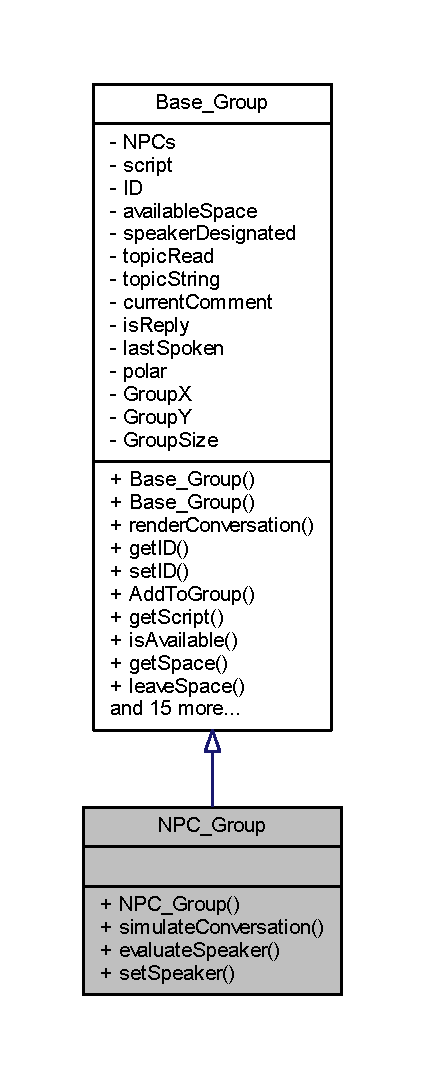
\includegraphics[width=204pt]{class_n_p_c___group__inherit__graph}
\end{center}
\end{figure}


Collaboration diagram for N\+P\+C\+\_\+\+Group\+:\nopagebreak
\begin{figure}[H]
\begin{center}
\leavevmode
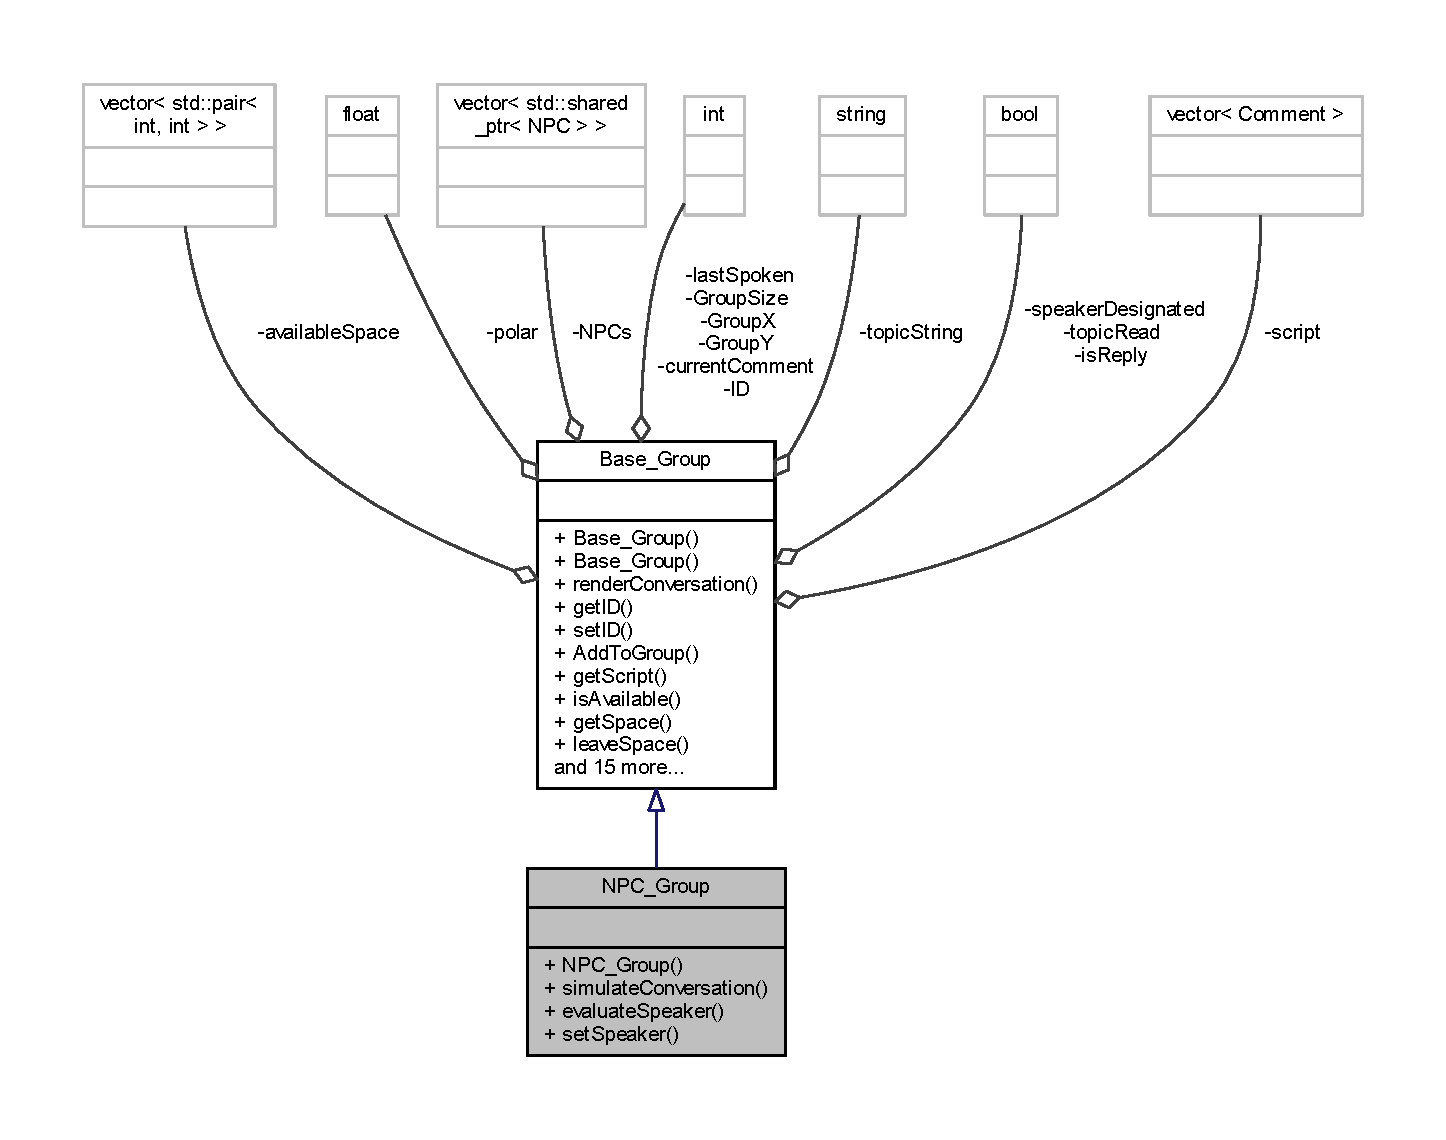
\includegraphics[width=350pt]{class_n_p_c___group__coll__graph}
\end{center}
\end{figure}
\subsection*{Public Member Functions}
\begin{DoxyCompactItemize}
\item 
\hyperlink{class_n_p_c___group_ab680383cc2de42390440bae5bae6b53e}{N\+P\+C\+\_\+\+Group} (int x, int y, int size, std\+::string t\+Box\+File, std\+::string npc\+File, S\+D\+L\+\_\+\+Renderer $\ast$renderer, \hyperlink{class_topic}{Topic} tp)
\item 
void \hyperlink{class_n_p_c___group_a139f16a36dba893743e227ea276fd5e7}{simulate\+Conversation} (S\+D\+L\+\_\+\+Renderer $\ast$renderer, bool time, std\+::string boredom\+Level, T\+T\+F\+\_\+\+Font $\ast$font)
\item 
bool \hyperlink{class_n_p_c___group_a2e0b8772b42985bd7e87359013918601}{evaluate\+Speaker} ()
\item 
void \hyperlink{class_n_p_c___group_a5c1f3d1ad1f50910bb912ed828615ff8}{set\+Speaker} (std\+::string boredom\+Level)
\end{DoxyCompactItemize}


\subsection{Detailed Description}
The \hyperlink{class_n_p_c___group}{N\+P\+C\+\_\+\+Group} class is designed to represent a maximum group of 6 \hyperlink{class_n_p_c}{N\+PC}\textquotesingle{}s. the specfied \hyperlink{class_n_p_c}{N\+PC}\textquotesingle{}s are initialised when the group is initialised. 

Definition at line 9 of file N\+P\+C\+\_\+\+Group.\+h.



\subsection{Constructor \& Destructor Documentation}
\mbox{\Hypertarget{class_n_p_c___group_ab680383cc2de42390440bae5bae6b53e}\label{class_n_p_c___group_ab680383cc2de42390440bae5bae6b53e}} 
\index{N\+P\+C\+\_\+\+Group@{N\+P\+C\+\_\+\+Group}!N\+P\+C\+\_\+\+Group@{N\+P\+C\+\_\+\+Group}}
\index{N\+P\+C\+\_\+\+Group@{N\+P\+C\+\_\+\+Group}!N\+P\+C\+\_\+\+Group@{N\+P\+C\+\_\+\+Group}}
\subsubsection{\texorpdfstring{N\+P\+C\+\_\+\+Group()}{NPC\_Group()}}
{\footnotesize\ttfamily N\+P\+C\+\_\+\+Group\+::\+N\+P\+C\+\_\+\+Group (\begin{DoxyParamCaption}\item[{int}]{x,  }\item[{int}]{y,  }\item[{int}]{size,  }\item[{std\+::string}]{t\+Box\+File,  }\item[{std\+::string}]{npc\+File,  }\item[{S\+D\+L\+\_\+\+Renderer $\ast$}]{renderer,  }\item[{\hyperlink{class_topic}{Topic}}]{tp }\end{DoxyParamCaption})}



Definition at line 3 of file N\+P\+C\+\_\+\+Group.\+cpp.


\begin{DoxyCode}
3                                                                                                            
              : \hyperlink{class_base___group_a96e70ee101d6430696f7b13b07190787}{Base\_Group}(x, y, size, tBoxFile, npcFile, renderer, tp)
4 \{\}
\end{DoxyCode}


\subsection{Member Function Documentation}
\mbox{\Hypertarget{class_n_p_c___group_a2e0b8772b42985bd7e87359013918601}\label{class_n_p_c___group_a2e0b8772b42985bd7e87359013918601}} 
\index{N\+P\+C\+\_\+\+Group@{N\+P\+C\+\_\+\+Group}!evaluate\+Speaker@{evaluate\+Speaker}}
\index{evaluate\+Speaker@{evaluate\+Speaker}!N\+P\+C\+\_\+\+Group@{N\+P\+C\+\_\+\+Group}}
\subsubsection{\texorpdfstring{evaluate\+Speaker()}{evaluateSpeaker()}}
{\footnotesize\ttfamily bool N\+P\+C\+\_\+\+Group\+::evaluate\+Speaker (\begin{DoxyParamCaption}{ }\end{DoxyParamCaption})\hspace{0.3cm}{\ttfamily [virtual]}}

This method checks if someone has already been selected to speak 

Reimplemented from \hyperlink{class_base___group_a8264ff598ce7e789c6419e2e6eef08fd}{Base\+\_\+\+Group}.



Definition at line 96 of file N\+P\+C\+\_\+\+Group.\+cpp.



References Base\+\_\+\+Group\+::get\+N\+P\+C\+List(), and Base\+\_\+\+Group\+::\+N\+P\+Cs.



Referenced by set\+Speaker().


\begin{DoxyCode}
97 \{
98     std::vector<std::shared\_ptr<NPC>> \hyperlink{class_base___group_a4757f3c06c73eea029f71b871c1d863e}{NPCs} = \hyperlink{class_base___group_a75eec9132aaf532b4429e0af76b31775}{getNPCList}();
99     \textcolor{keywordflow}{for} (\textcolor{keywordtype}{int} i = 0; i < NPCs.size(); i++)
100     \{
101         \textcolor{comment}{// if there is already a speaker return true}
102         \textcolor{keywordflow}{if} (NPCs[i]->getSpeaking())
103             \textcolor{keywordflow}{return} \textcolor{keyword}{true};
104     \}
105     \textcolor{keywordflow}{return} \textcolor{keyword}{false};
106 \}
\end{DoxyCode}
\mbox{\Hypertarget{class_n_p_c___group_a5c1f3d1ad1f50910bb912ed828615ff8}\label{class_n_p_c___group_a5c1f3d1ad1f50910bb912ed828615ff8}} 
\index{N\+P\+C\+\_\+\+Group@{N\+P\+C\+\_\+\+Group}!set\+Speaker@{set\+Speaker}}
\index{set\+Speaker@{set\+Speaker}!N\+P\+C\+\_\+\+Group@{N\+P\+C\+\_\+\+Group}}
\subsubsection{\texorpdfstring{set\+Speaker()}{setSpeaker()}}
{\footnotesize\ttfamily void N\+P\+C\+\_\+\+Group\+::set\+Speaker (\begin{DoxyParamCaption}\item[{std\+::string}]{boredom\+Level }\end{DoxyParamCaption})\hspace{0.3cm}{\ttfamily [virtual]}}

set\textquotesingle{}s the next speaker of the conversation, also applys boredom to the other N\+P\+Cs 

Reimplemented from \hyperlink{class_base___group_ae35b3719076cf40d6577b4ae3779758c}{Base\+\_\+\+Group}.



Definition at line 111 of file N\+P\+C\+\_\+\+Group.\+cpp.



References evaluate\+Speaker(), Base\+\_\+\+Group\+::get\+I\+D(), Base\+\_\+\+Group\+::get\+N\+P\+C\+List(), Base\+\_\+\+Group\+::\+Get\+Random\+Number(), and Base\+\_\+\+Group\+::\+N\+P\+Cs.



Referenced by simulate\+Conversation().


\begin{DoxyCode}
112 \{
113     \textcolor{keywordflow}{if} (!\hyperlink{class_n_p_c___group_a2e0b8772b42985bd7e87359013918601}{evaluateSpeaker}()) \{
114         \textcolor{comment}{// get a random number}
115         \textcolor{keywordtype}{int} r = \hyperlink{class_base___group_a3864a2806457151363344051f2814389}{GetRandomNumber}();
116         std::vector<std::shared\_ptr<NPC>> \hyperlink{class_base___group_a4757f3c06c73eea029f71b871c1d863e}{NPCs} = \hyperlink{class_base___group_a75eec9132aaf532b4429e0af76b31775}{getNPCList}();
117         \textcolor{keywordflow}{for} (\textcolor{keywordtype}{int} i = 0; i < NPCs.size(); i++)
118         \{
119             \textcolor{comment}{// if the NPC does not match the chosen speaker, increment their boredom levels}
120             \textcolor{keywordflow}{if} (NPCs[i]->\hyperlink{class_base___group_a7299ae154b26d741ac2f6f794bc3a544}{getID}() != NPCs[r]->getID())
121             \{
122                 \textcolor{keywordtype}{int} bored = NPCs[i]->getBoredom() + 1;
123                 NPCs[i]->setBoredom(bored);
124 
125                 \textcolor{comment}{// if the boredom level surpasses the global boredom threshhold, set the NPC to idle}
126                 \textcolor{keywordflow}{if} (NPCs[i]->getBoredom() > atoi(boredomLevel.c\_str()))
127                 \{
128                     NPCs[i]->setIdle(\textcolor{keyword}{true});
129                 \}
130             \}
131         \}
132 
133         \textcolor{comment}{// set the speakers boredom to 0}
134         NPCs[r]->setSpeaking(\textcolor{keyword}{true});
135         NPCs[r]->setBoredom(0);
136     \}
137 \}
\end{DoxyCode}
\mbox{\Hypertarget{class_n_p_c___group_a139f16a36dba893743e227ea276fd5e7}\label{class_n_p_c___group_a139f16a36dba893743e227ea276fd5e7}} 
\index{N\+P\+C\+\_\+\+Group@{N\+P\+C\+\_\+\+Group}!simulate\+Conversation@{simulate\+Conversation}}
\index{simulate\+Conversation@{simulate\+Conversation}!N\+P\+C\+\_\+\+Group@{N\+P\+C\+\_\+\+Group}}
\subsubsection{\texorpdfstring{simulate\+Conversation()}{simulateConversation()}}
{\footnotesize\ttfamily void N\+P\+C\+\_\+\+Group\+::simulate\+Conversation (\begin{DoxyParamCaption}\item[{S\+D\+L\+\_\+\+Renderer $\ast$}]{renderer,  }\item[{bool}]{time,  }\item[{std\+::string}]{boredom\+Level,  }\item[{T\+T\+F\+\_\+\+Font $\ast$}]{font }\end{DoxyParamCaption})\hspace{0.3cm}{\ttfamily [virtual]}}

This method is the implementation of Algorithm 1, which makes use of a script and anonymous N\+P\+Cs 

Reimplemented from \hyperlink{class_base___group_aa5080b6388c5974394bf326ce80bfa91}{Base\+\_\+\+Group}.



Definition at line 9 of file N\+P\+C\+\_\+\+Group.\+cpp.



References Base\+\_\+\+Group\+::get\+Is\+Reply(), Base\+\_\+\+Group\+::get\+Last\+Spoken(), Base\+\_\+\+Group\+::get\+N\+P\+C\+List(), Base\+\_\+\+Group\+::get\+Polar(), Base\+\_\+\+Group\+::get\+Script(), Base\+\_\+\+Group\+::\+N\+P\+Cs, Base\+\_\+\+Group\+::set\+Is\+Reply(), Base\+\_\+\+Group\+::set\+Last\+Spoken(), Base\+\_\+\+Group\+::set\+Polar(), set\+Speaker(), and Base\+\_\+\+Group\+::update\+Script().


\begin{DoxyCode}
10 \{
11     \textcolor{comment}{// if the neccecary amount of time has passed, run the simulation code}
12     \textcolor{keywordflow}{if} (time)
13     \{
14         \textcolor{comment}{// set the speaker of the conversation}
15         \hyperlink{class_n_p_c___group_a5c1f3d1ad1f50910bb912ed828615ff8}{setSpeaker}(boredomLevel);
16 
17         std::vector<std::shared\_ptr<NPC>> \hyperlink{class_base___group_a4757f3c06c73eea029f71b871c1d863e}{NPCs} = \hyperlink{class_base___group_a75eec9132aaf532b4429e0af76b31775}{getNPCList}();
18         \textcolor{keywordflow}{for} (\textcolor{keywordtype}{int} i = 0; i < NPCs.size(); i++)
19         \{
20             std::shared\_ptr<NPC> npc = NPCs[i];
21             \textcolor{comment}{//check if the script has ended}
22             \textcolor{keywordflow}{if} (\hyperlink{class_base___group_a48dadfbc8cdefca9bdd2c42b99115ad8}{getScript}().size() > 0)
23             \{
24                 \textcolor{comment}{//ignore all idle NPCs}
25                 \textcolor{keywordflow}{if} (!npc->getIdle())
26                 \{
27                     \textcolor{comment}{//get the NPC who is set to speak}
28                     \textcolor{keywordflow}{if} (npc->getSpeaking())
29                     \{
30                         \textcolor{comment}{// if the NPC is not reading, then assign him a fresh comment}
31                         \textcolor{keywordflow}{if} (!npc->getReading())
32                         \{
33                             npc->LoadBox(renderer);
34                             npc->setText(\hyperlink{class_base___group_a48dadfbc8cdefca9bdd2c42b99115ad8}{getScript}()[0].getBody());
35                             npc->prepareComment(\hyperlink{class_base___group_a48dadfbc8cdefca9bdd2c42b99115ad8}{getScript}()[0].getBody(), font);
36                             npc->setReading(\textcolor{keyword}{true});
37                         \}
38 
39                         \textcolor{keywordflow}{if} (npc->getReading())
40                         \{
41                             \textcolor{comment}{// get the number of lines thats is being rendered to the screen}
42                             \textcolor{keywordtype}{int} lines = npc->getLinesToRender();
43                             \textcolor{keywordflow}{if} (npc->getCurrentLine() < lines)
44                             \{
45                                 \textcolor{comment}{// load the NPCs comment as a texture}
46                                 npc->LoadComment(renderer, npc->getCurrentLine(), font);
47                                 npc->setCurrentLine(npc->getCurrentLine() + 1);
48                             \}
49                             \textcolor{keywordflow}{else}
50                             \{
51                                 \textcolor{keywordflow}{if} (\hyperlink{class_base___group_a878700b51979d0acd3eb83cdfa4c0449}{getIsReply}())
52                                 \{
53                                     \textcolor{comment}{// if this comment is a reply, apply the sentiment score to the
       previous speaker}
54                                     \textcolor{keywordflow}{if} (\hyperlink{class_base___group_a8fb88afb104365ec23447ee1f3649b4c}{getLastSpoken}() < 
      \hyperlink{class_base___group_a75eec9132aaf532b4429e0af76b31775}{getNPCList}().size())
55                                         NPCs[\hyperlink{class_base___group_a8fb88afb104365ec23447ee1f3649b4c}{getLastSpoken}()]->applyEmotionLevel(
      \hyperlink{class_base___group_a57cd8ebf1eee11eab80816ee87223f36}{getPolar}());
56                                 \}
57 
58                                 \textcolor{comment}{//the NPC has finished reading, so set him to not speak, and update
       conversation values}
59                                 npc->setSpeaking(\textcolor{keyword}{false});
60                                 npc->setReading(\textcolor{keyword}{false});
61                                 \hyperlink{class_base___group_aebe2b457ac29aefcc7105908a61460c8}{setIsReply}(\hyperlink{class_base___group_a48dadfbc8cdefca9bdd2c42b99115ad8}{getScript}()[0].getReply());
62                                 \hyperlink{class_base___group_a36ef627854f502a064fca8aea44a22fe}{setPolar}(\hyperlink{class_base___group_a48dadfbc8cdefca9bdd2c42b99115ad8}{getScript}()[0].getPolarity());
63                                 \hyperlink{class_base___group_a07e58c944f222f5c3d3b33c8adf83d14}{setLastSpoken}(i);
64                                 npc->setCurrentLine(0);
65                                 \hyperlink{class_base___group_a8c16feac44492aa68f4ee758662892c8}{updateScript}();
66                                 \hyperlink{class_n_p_c___group_a5c1f3d1ad1f50910bb912ed828615ff8}{setSpeaker}(boredomLevel);
67                             \}
68                         \}
69                     \}
70                 \}
71                 \textcolor{keywordflow}{else}
72                 \{
73                     \textcolor{comment}{// if the NPC is idle, he is not part of the conversation, and cant speak}
74                     \textcolor{keywordflow}{if} (npc->getSpeaking())
75                     \{
76                         npc->setSpeaking(\textcolor{keyword}{false});
77                     \}
78                 \}
79             \}
80             \textcolor{keywordflow}{else}
81             \{
82                 \textcolor{comment}{// if there is no script there is not conversation, so there cant be a speaker.}
83                 npc->setSpeaking(\textcolor{keyword}{false});
84                 npc->setReading(\textcolor{keyword}{false});
85                 \hyperlink{class_base___group_a07e58c944f222f5c3d3b33c8adf83d14}{setLastSpoken}(i);
86                 npc->setCurrentLine(0);
87                 npc->freeBox();
88             \}
89         \}
90     \}
91 \}
\end{DoxyCode}


The documentation for this class was generated from the following files\+:\begin{DoxyCompactItemize}
\item 
C\+:/\+Users/\+Kyle Tuckey/\+Documents/\+Final Year Project/\+Social\+\_\+\+N\+P\+C\+S/\+Social\+\_\+\+N\+P\+C\+S/\hyperlink{_n_p_c___group_8h}{N\+P\+C\+\_\+\+Group.\+h}\item 
C\+:/\+Users/\+Kyle Tuckey/\+Documents/\+Final Year Project/\+Social\+\_\+\+N\+P\+C\+S/\+Social\+\_\+\+N\+P\+C\+S/\hyperlink{_n_p_c___group_8cpp}{N\+P\+C\+\_\+\+Group.\+cpp}\end{DoxyCompactItemize}

\hypertarget{classcomments_1_1_object}{}\section{comments.\+Object Class Reference}
\label{classcomments_1_1_object}\index{comments.\+Object@{comments.\+Object}}


Collaboration diagram for comments.\+Object\+:\nopagebreak
\begin{figure}[H]
\begin{center}
\leavevmode
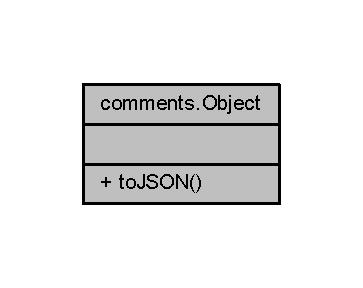
\includegraphics[width=174pt]{classcomments_1_1_object__coll__graph}
\end{center}
\end{figure}
\subsection*{Public Member Functions}
\begin{DoxyCompactItemize}
\item 
def \hyperlink{classcomments_1_1_object_a28ae66a09cca16c0c2ef7f26a3add15e}{to\+J\+S\+ON} (self)
\end{DoxyCompactItemize}


\subsection{Detailed Description}


Definition at line 9 of file comments.\+py.



\subsection{Member Function Documentation}
\mbox{\Hypertarget{classcomments_1_1_object_a28ae66a09cca16c0c2ef7f26a3add15e}\label{classcomments_1_1_object_a28ae66a09cca16c0c2ef7f26a3add15e}} 
\index{comments\+::\+Object@{comments\+::\+Object}!to\+J\+S\+ON@{to\+J\+S\+ON}}
\index{to\+J\+S\+ON@{to\+J\+S\+ON}!comments\+::\+Object@{comments\+::\+Object}}
\subsubsection{\texorpdfstring{to\+J\+S\+O\+N()}{toJSON()}}
{\footnotesize\ttfamily def comments.\+Object.\+to\+J\+S\+ON (\begin{DoxyParamCaption}\item[{}]{self }\end{DoxyParamCaption})}



Definition at line 10 of file comments.\+py.


\begin{DoxyCode}
10     \textcolor{keyword}{def }toJSON(self):
11         \textcolor{keywordflow}{return} json.dumps(self, default=\textcolor{keyword}{lambda} o: o.\_\_dict\_\_, 
12             sort\_keys=\textcolor{keyword}{True}, indent=4)   
\end{DoxyCode}


The documentation for this class was generated from the following file\+:\begin{DoxyCompactItemize}
\item 
C\+:/\+Users/\+Kyle Tuckey/\+Documents/\+Final Year Project/\+Social\+\_\+\+N\+P\+C\+S/\+Social\+\_\+\+N\+P\+C\+S/\hyperlink{comments_8py}{comments.\+py}\end{DoxyCompactItemize}

\hypertarget{class_python_handler}{}\section{Python\+Handler Class Reference}
\label{class_python_handler}\index{Python\+Handler@{Python\+Handler}}


{\ttfamily \#include $<$Python\+Handler.\+h$>$}



Collaboration diagram for Python\+Handler\+:\nopagebreak
\begin{figure}[H]
\begin{center}
\leavevmode
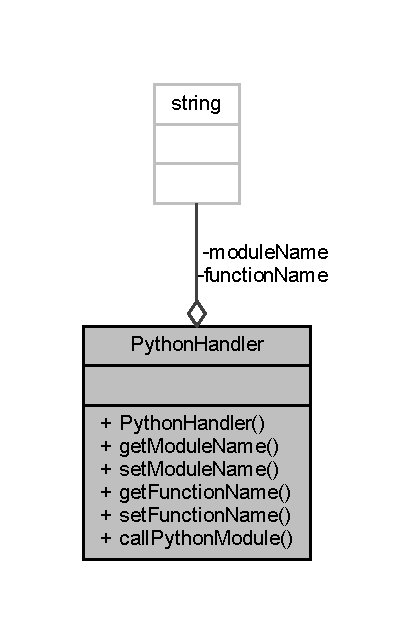
\includegraphics[width=199pt]{class_python_handler__coll__graph}
\end{center}
\end{figure}
\subsection*{Public Member Functions}
\begin{DoxyCompactItemize}
\item 
\hyperlink{class_python_handler_ac49f0f52604ab7afb9443712bf1c2cd0}{Python\+Handler} (std\+::string module, std\+::string function)
\item 
std\+::string \hyperlink{class_python_handler_acf20183155762af98d1f8804881cddb4}{get\+Module\+Name} ()
\item 
void \hyperlink{class_python_handler_a035cda1c3987043041c7aeb8e3440f04}{set\+Module\+Name} (std\+::string module)
\item 
std\+::string \hyperlink{class_python_handler_a60186d0ff375491ad5d91c7448c29288}{get\+Function\+Name} ()
\item 
void \hyperlink{class_python_handler_a640d790693c476a5bdd87050c7416ff0}{set\+Function\+Name} (std\+::string function)
\item 
void \hyperlink{class_python_handler_ac60ae844922ca438081e1f8cc0164b45}{call\+Python\+Module} ()
\begin{DoxyCompactList}\small\item\em Call the python script to gather comments. \end{DoxyCompactList}\end{DoxyCompactItemize}
\subsection*{Private Attributes}
\begin{DoxyCompactItemize}
\item 
std\+::string \hyperlink{class_python_handler_ae29ce86e7c2dce2340caa90ba1d6ac72}{module\+Name}
\item 
std\+::string \hyperlink{class_python_handler_a5946996068756c245e023cfe7e77f034}{function\+Name}
\end{DoxyCompactItemize}


\subsection{Detailed Description}
Wrapper to handle the C/\+Python api functionality, in charge of calling the external python scripts 

Definition at line 7 of file Python\+Handler.\+h.



\subsection{Constructor \& Destructor Documentation}
\mbox{\Hypertarget{class_python_handler_ac49f0f52604ab7afb9443712bf1c2cd0}\label{class_python_handler_ac49f0f52604ab7afb9443712bf1c2cd0}} 
\index{Python\+Handler@{Python\+Handler}!Python\+Handler@{Python\+Handler}}
\index{Python\+Handler@{Python\+Handler}!Python\+Handler@{Python\+Handler}}
\subsubsection{\texorpdfstring{Python\+Handler()}{PythonHandler()}}
{\footnotesize\ttfamily Python\+Handler\+::\+Python\+Handler (\begin{DoxyParamCaption}\item[{std\+::string}]{module,  }\item[{std\+::string}]{function }\end{DoxyParamCaption})}



Definition at line 3 of file Python\+Handler.\+cpp.



References set\+Function\+Name(), and set\+Module\+Name().


\begin{DoxyCode}
4 \{
5     \hyperlink{class_python_handler_a035cda1c3987043041c7aeb8e3440f04}{setModuleName}(module);
6     \hyperlink{class_python_handler_a640d790693c476a5bdd87050c7416ff0}{setFunctionName}(\textcolor{keyword}{function});
7 \}
\end{DoxyCode}


\subsection{Member Function Documentation}
\mbox{\Hypertarget{class_python_handler_ac60ae844922ca438081e1f8cc0164b45}\label{class_python_handler_ac60ae844922ca438081e1f8cc0164b45}} 
\index{Python\+Handler@{Python\+Handler}!call\+Python\+Module@{call\+Python\+Module}}
\index{call\+Python\+Module@{call\+Python\+Module}!Python\+Handler@{Python\+Handler}}
\subsubsection{\texorpdfstring{call\+Python\+Module()}{callPythonModule()}}
{\footnotesize\ttfamily void Python\+Handler\+::call\+Python\+Module (\begin{DoxyParamCaption}{ }\end{DoxyParamCaption})}



Call the python script to gather comments. 



Definition at line 29 of file Python\+Handler.\+cpp.



References function\+Name, and module\+Name.



Referenced by main().


\begin{DoxyCode}
30 \{
31     \textcolor{keywordflow}{try}
32     \{
33         \textcolor{comment}{//Begin python}
34         Py\_Initialize();
35 
36         \textcolor{comment}{//Call the python module}
37         PyObject* module = PyImport\_ImportModule(\hyperlink{class_python_handler_ae29ce86e7c2dce2340caa90ba1d6ac72}{moduleName}.c\_str());
38         \textcolor{keywordflow}{if} (module == 0)
39         \{
40             PyErr\_Print();
41             printf(\textcolor{stringliteral}{"Couldn't find python module"});
42         \}
43 
44         \textcolor{comment}{//Create a dictionary of the function's inside the module}
45         PyObject* comDict = PyModule\_GetDict(module);
46 
47         \textcolor{comment}{//State the specified function name from the dictionary}
48         PyObject* func = PyDict\_GetItemString(comDict, \hyperlink{class_python_handler_a5946996068756c245e023cfe7e77f034}{functionName}.c\_str());
49 
50         \textcolor{comment}{//State the argument's you want NOTE: currently only work's with functions with 0 arguments}
51         PyObject* args = PyTuple\_New(0);
52 
53         \textcolor{comment}{//Call the object}
54         PyObject* result = PyObject\_CallObject(func, args);
55         \textcolor{keywordflow}{if} (result == NULL)
56         \{
57             printf(\textcolor{stringliteral}{"Calling function failed"});
58         \}
59 
60         \textcolor{comment}{//Print any errors}
61         PyErr\_Print();
62 
63         \textcolor{comment}{//Clean up the pointer's}
64         Py\_DECREF(module);
65         Py\_DECREF(comDict);
66         Py\_DECREF(func);
67         Py\_DECREF(args);
68         Py\_DECREF(result);
69 
70         \textcolor{comment}{//End the python process}
71         Py\_Finalize();
72     \}
73     \textcolor{keywordflow}{catch} (...) \{
74         PyObject *ptype, *pvalue, *ptraceback;
75         PyErr\_Fetch(&ptype, &pvalue, &ptraceback);
76 
77         \textcolor{keywordtype}{char}* pStrErrorMessage = \_PyUnicode\_AsString(pvalue);
78 
79         Py\_DECREF(ptype);
80         Py\_DECREF(pvalue);
81         Py\_DECREF(ptraceback);
82     \}
83 \}
\end{DoxyCode}
\mbox{\Hypertarget{class_python_handler_a60186d0ff375491ad5d91c7448c29288}\label{class_python_handler_a60186d0ff375491ad5d91c7448c29288}} 
\index{Python\+Handler@{Python\+Handler}!get\+Function\+Name@{get\+Function\+Name}}
\index{get\+Function\+Name@{get\+Function\+Name}!Python\+Handler@{Python\+Handler}}
\subsubsection{\texorpdfstring{get\+Function\+Name()}{getFunctionName()}}
{\footnotesize\ttfamily std\+::string Python\+Handler\+::get\+Function\+Name (\begin{DoxyParamCaption}{ }\end{DoxyParamCaption})}



Definition at line 19 of file Python\+Handler.\+cpp.



References function\+Name.


\begin{DoxyCode}
20 \{
21     \textcolor{keywordflow}{return} \hyperlink{class_python_handler_a5946996068756c245e023cfe7e77f034}{functionName};
22 \}
\end{DoxyCode}
\mbox{\Hypertarget{class_python_handler_acf20183155762af98d1f8804881cddb4}\label{class_python_handler_acf20183155762af98d1f8804881cddb4}} 
\index{Python\+Handler@{Python\+Handler}!get\+Module\+Name@{get\+Module\+Name}}
\index{get\+Module\+Name@{get\+Module\+Name}!Python\+Handler@{Python\+Handler}}
\subsubsection{\texorpdfstring{get\+Module\+Name()}{getModuleName()}}
{\footnotesize\ttfamily std\+::string Python\+Handler\+::get\+Module\+Name (\begin{DoxyParamCaption}{ }\end{DoxyParamCaption})}



Definition at line 9 of file Python\+Handler.\+cpp.



References module\+Name.


\begin{DoxyCode}
10 \{
11     \textcolor{keywordflow}{return} \hyperlink{class_python_handler_ae29ce86e7c2dce2340caa90ba1d6ac72}{moduleName};
12 \}
\end{DoxyCode}
\mbox{\Hypertarget{class_python_handler_a640d790693c476a5bdd87050c7416ff0}\label{class_python_handler_a640d790693c476a5bdd87050c7416ff0}} 
\index{Python\+Handler@{Python\+Handler}!set\+Function\+Name@{set\+Function\+Name}}
\index{set\+Function\+Name@{set\+Function\+Name}!Python\+Handler@{Python\+Handler}}
\subsubsection{\texorpdfstring{set\+Function\+Name()}{setFunctionName()}}
{\footnotesize\ttfamily void Python\+Handler\+::set\+Function\+Name (\begin{DoxyParamCaption}\item[{std\+::string}]{function }\end{DoxyParamCaption})}



Definition at line 24 of file Python\+Handler.\+cpp.



References function\+Name.



Referenced by Python\+Handler().


\begin{DoxyCode}
25 \{
26     \hyperlink{class_python_handler_a5946996068756c245e023cfe7e77f034}{functionName} = funcName;
27 \}
\end{DoxyCode}
\mbox{\Hypertarget{class_python_handler_a035cda1c3987043041c7aeb8e3440f04}\label{class_python_handler_a035cda1c3987043041c7aeb8e3440f04}} 
\index{Python\+Handler@{Python\+Handler}!set\+Module\+Name@{set\+Module\+Name}}
\index{set\+Module\+Name@{set\+Module\+Name}!Python\+Handler@{Python\+Handler}}
\subsubsection{\texorpdfstring{set\+Module\+Name()}{setModuleName()}}
{\footnotesize\ttfamily void Python\+Handler\+::set\+Module\+Name (\begin{DoxyParamCaption}\item[{std\+::string}]{module }\end{DoxyParamCaption})}



Definition at line 14 of file Python\+Handler.\+cpp.



References module\+Name.



Referenced by Python\+Handler().


\begin{DoxyCode}
15 \{
16     \hyperlink{class_python_handler_ae29ce86e7c2dce2340caa90ba1d6ac72}{moduleName} = modName;
17 \}
\end{DoxyCode}


\subsection{Member Data Documentation}
\mbox{\Hypertarget{class_python_handler_a5946996068756c245e023cfe7e77f034}\label{class_python_handler_a5946996068756c245e023cfe7e77f034}} 
\index{Python\+Handler@{Python\+Handler}!function\+Name@{function\+Name}}
\index{function\+Name@{function\+Name}!Python\+Handler@{Python\+Handler}}
\subsubsection{\texorpdfstring{function\+Name}{functionName}}
{\footnotesize\ttfamily std\+::string Python\+Handler\+::function\+Name\hspace{0.3cm}{\ttfamily [private]}}



Definition at line 22 of file Python\+Handler.\+h.



Referenced by call\+Python\+Module(), get\+Function\+Name(), and set\+Function\+Name().

\mbox{\Hypertarget{class_python_handler_ae29ce86e7c2dce2340caa90ba1d6ac72}\label{class_python_handler_ae29ce86e7c2dce2340caa90ba1d6ac72}} 
\index{Python\+Handler@{Python\+Handler}!module\+Name@{module\+Name}}
\index{module\+Name@{module\+Name}!Python\+Handler@{Python\+Handler}}
\subsubsection{\texorpdfstring{module\+Name}{moduleName}}
{\footnotesize\ttfamily std\+::string Python\+Handler\+::module\+Name\hspace{0.3cm}{\ttfamily [private]}}



Definition at line 21 of file Python\+Handler.\+h.



Referenced by call\+Python\+Module(), get\+Module\+Name(), and set\+Module\+Name().



The documentation for this class was generated from the following files\+:\begin{DoxyCompactItemize}
\item 
C\+:/\+Users/\+Kyle Tuckey/\+Documents/\+Final Year Project/\+Social\+\_\+\+N\+P\+C\+S/\+Social\+\_\+\+N\+P\+C\+S/\hyperlink{_python_handler_8h}{Python\+Handler.\+h}\item 
C\+:/\+Users/\+Kyle Tuckey/\+Documents/\+Final Year Project/\+Social\+\_\+\+N\+P\+C\+S/\+Social\+\_\+\+N\+P\+C\+S/\hyperlink{_python_handler_8cpp}{Python\+Handler.\+cpp}\end{DoxyCompactItemize}

\hypertarget{class_resource_data}{}\section{Resource\+Data Class Reference}
\label{class_resource_data}\index{Resource\+Data@{Resource\+Data}}


{\ttfamily \#include $<$Resource\+Data.\+h$>$}



Collaboration diagram for Resource\+Data\+:\nopagebreak
\begin{figure}[H]
\begin{center}
\leavevmode
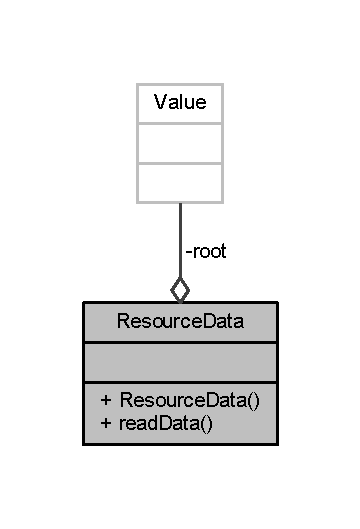
\includegraphics[width=173pt]{class_resource_data__coll__graph}
\end{center}
\end{figure}
\subsection*{Public Member Functions}
\begin{DoxyCompactItemize}
\item 
\hyperlink{class_resource_data_afa0fffd6caad715b697c1b3a388c975d}{Resource\+Data} (std\+::ifstream file)
\item 
std\+::string \hyperlink{class_resource_data_a2e18ba115b2598590c15a16240542948}{read\+Data} (std\+::string key)
\end{DoxyCompactItemize}
\subsection*{Private Attributes}
\begin{DoxyCompactItemize}
\item 
Json\+::\+Value \hyperlink{class_resource_data_a0e9ea464b4a3fae26f68d01e344008fb}{root}
\end{DoxyCompactItemize}


\subsection{Detailed Description}
Reads in the resource data for the application 

Definition at line 8 of file Resource\+Data.\+h.



\subsection{Constructor \& Destructor Documentation}
\mbox{\Hypertarget{class_resource_data_afa0fffd6caad715b697c1b3a388c975d}\label{class_resource_data_afa0fffd6caad715b697c1b3a388c975d}} 
\index{Resource\+Data@{Resource\+Data}!Resource\+Data@{Resource\+Data}}
\index{Resource\+Data@{Resource\+Data}!Resource\+Data@{Resource\+Data}}
\subsubsection{\texorpdfstring{Resource\+Data()}{ResourceData()}}
{\footnotesize\ttfamily Resource\+Data\+::\+Resource\+Data (\begin{DoxyParamCaption}\item[{std\+::ifstream}]{file }\end{DoxyParamCaption})}



Definition at line 5 of file Resource\+Data.\+cpp.



References root.


\begin{DoxyCode}
6 \{
7     file >> \hyperlink{class_resource_data_a0e9ea464b4a3fae26f68d01e344008fb}{root};
8 \}
\end{DoxyCode}


\subsection{Member Function Documentation}
\mbox{\Hypertarget{class_resource_data_a2e18ba115b2598590c15a16240542948}\label{class_resource_data_a2e18ba115b2598590c15a16240542948}} 
\index{Resource\+Data@{Resource\+Data}!read\+Data@{read\+Data}}
\index{read\+Data@{read\+Data}!Resource\+Data@{Resource\+Data}}
\subsubsection{\texorpdfstring{read\+Data()}{readData()}}
{\footnotesize\ttfamily std\+::string Resource\+Data\+::read\+Data (\begin{DoxyParamCaption}\item[{std\+::string}]{key }\end{DoxyParamCaption})}



Definition at line 10 of file Resource\+Data.\+cpp.



References root.



Referenced by main().


\begin{DoxyCode}
11 \{
12     \textcolor{keywordflow}{return} \hyperlink{class_resource_data_a0e9ea464b4a3fae26f68d01e344008fb}{root}[key].asString();
13 \}
\end{DoxyCode}


\subsection{Member Data Documentation}
\mbox{\Hypertarget{class_resource_data_a0e9ea464b4a3fae26f68d01e344008fb}\label{class_resource_data_a0e9ea464b4a3fae26f68d01e344008fb}} 
\index{Resource\+Data@{Resource\+Data}!root@{root}}
\index{root@{root}!Resource\+Data@{Resource\+Data}}
\subsubsection{\texorpdfstring{root}{root}}
{\footnotesize\ttfamily Json\+::\+Value Resource\+Data\+::root\hspace{0.3cm}{\ttfamily [private]}}



Definition at line 15 of file Resource\+Data.\+h.



Referenced by read\+Data(), and Resource\+Data().



The documentation for this class was generated from the following files\+:\begin{DoxyCompactItemize}
\item 
C\+:/\+Users/\+Kyle Tuckey/\+Documents/\+Final Year Project/\+Social\+\_\+\+N\+P\+C\+S/\+Social\+\_\+\+N\+P\+C\+S/\hyperlink{_resource_data_8h}{Resource\+Data.\+h}\item 
C\+:/\+Users/\+Kyle Tuckey/\+Documents/\+Final Year Project/\+Social\+\_\+\+N\+P\+C\+S/\+Social\+\_\+\+N\+P\+C\+S/\hyperlink{_resource_data_8cpp}{Resource\+Data.\+cpp}\end{DoxyCompactItemize}

\hypertarget{class_room}{}\section{Room Class Reference}
\label{class_room}\index{Room@{Room}}


{\ttfamily \#include $<$Room.\+h$>$}



Collaboration diagram for Room\+:\nopagebreak
\begin{figure}[H]
\begin{center}
\leavevmode
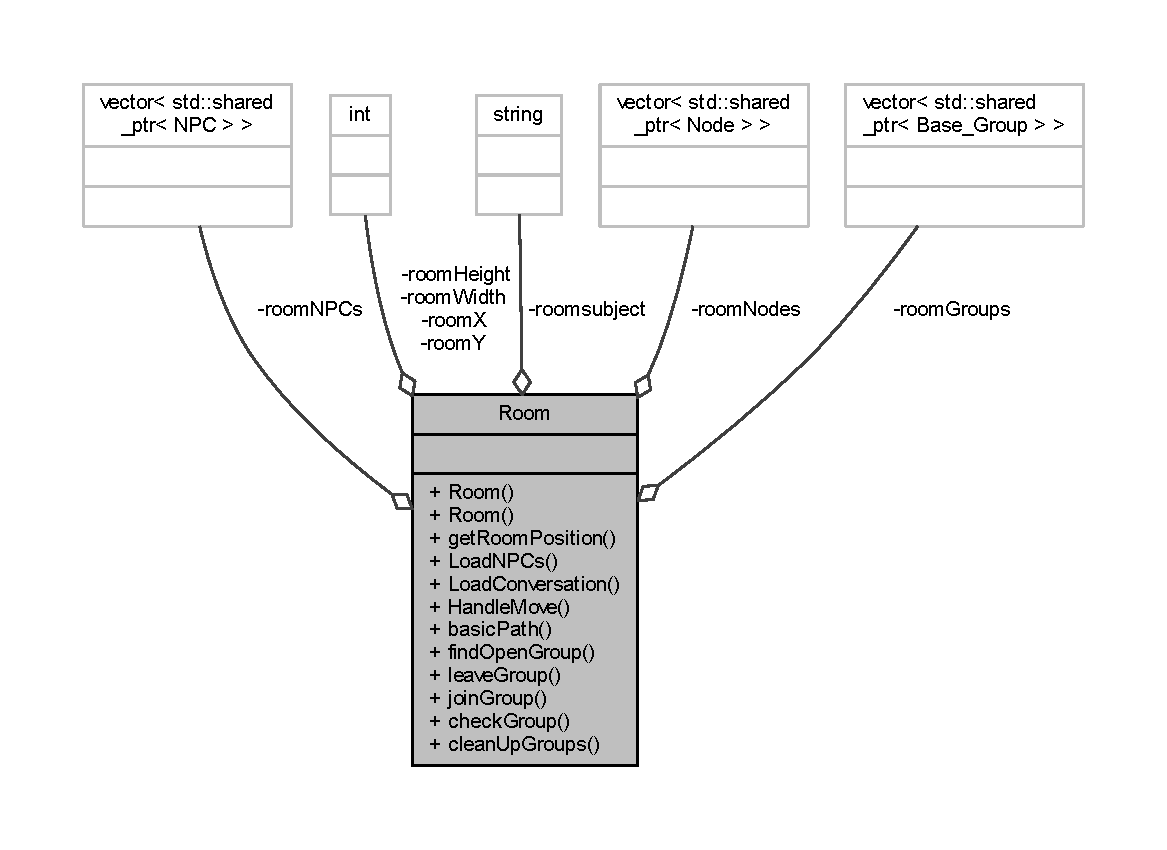
\includegraphics[width=350pt]{class_room__coll__graph}
\end{center}
\end{figure}
\subsection*{Public Member Functions}
\begin{DoxyCompactItemize}
\item 
\hyperlink{class_room_ac6ef93a7d9c3e1d624e025058d5f16ff}{Room} ()
\item 
\hyperlink{class_room_a2f37c248b2d9882531e01ab675ea54f0}{Room} (int group\+Num, int x, int y, int width, int height, std\+::string N\+P\+C\+Sprite, std\+::string Text\+Box\+Sprite, S\+D\+L\+\_\+\+Renderer $\ast$renderer, \hyperlink{class_group}{Group} grp)
\item 
std\+::pair$<$ int, int $>$ \hyperlink{class_room_ac57c28e2c1048649e816f731f63f9daf}{get\+Room\+Position} (int pos)
\begin{DoxyCompactList}\small\item\em return the rooms positions \end{DoxyCompactList}\item 
void \hyperlink{class_room_a876301b35488a7dc07bde00f0b701f9a}{Load\+N\+P\+Cs} (S\+D\+L\+\_\+\+Renderer $\ast$renderer)
\begin{DoxyCompactList}\small\item\em render the N\+P\+Cs to the scene \end{DoxyCompactList}\item 
void \hyperlink{class_room_a85476905ce9262f07dbb4a25f9729545}{Load\+Conversation} (S\+D\+L\+\_\+\+Renderer $\ast$renderer, bool time, std\+::string boredom\+Level, T\+T\+F\+\_\+\+Font $\ast$font)
\begin{DoxyCompactList}\small\item\em render the \hyperlink{class_n_p_c}{N\+PC} conversations in the room \end{DoxyCompactList}\item 
void \hyperlink{class_room_ae40e34ac3588b2dfe2be6c5d66e20552}{Handle\+Move} (S\+D\+L\+\_\+\+Renderer $\ast$renderer)
\begin{DoxyCompactList}\small\item\em handle \hyperlink{class_n_p_c}{N\+PC} movement \end{DoxyCompactList}\item 
void \hyperlink{class_room_af25611552daa6c57915a0b0c98c40a8a}{basic\+Path} (std\+::shared\+\_\+ptr$<$ \hyperlink{class_n_p_c}{N\+PC} $>$ npc, S\+D\+L\+\_\+\+Renderer $\ast$renderer)
\begin{DoxyCompactList}\small\item\em generate a basic path for the \hyperlink{class_n_p_c}{N\+PC} to follow \end{DoxyCompactList}\item 
int \hyperlink{class_room_a7d4ef90e7eb605f2c198b28175900d45}{find\+Open\+Group} (int exclude)
\begin{DoxyCompactList}\small\item\em return the id of any open groups \end{DoxyCompactList}\item 
void \hyperlink{class_room_af6bdbbf116aeafe290a31990a1124562}{leave\+Group} (std\+::shared\+\_\+ptr$<$ \hyperlink{class_n_p_c}{N\+PC} $>$ npc)
\begin{DoxyCompactList}\small\item\em remove an npc from a group \end{DoxyCompactList}\item 
void \hyperlink{class_room_a8cf434656fbafb4d65ee47c33db5c8ed}{join\+Group} (std\+::shared\+\_\+ptr$<$ \hyperlink{class_n_p_c}{N\+PC} $>$ npc, int id)
\begin{DoxyCompactList}\small\item\em add an npc to a group \end{DoxyCompactList}\item 
bool \hyperlink{class_room_a0c1e8e264493205408553a998a068b29}{check\+Group} (int id)
\begin{DoxyCompactList}\small\item\em check if any groups have finished conversing \end{DoxyCompactList}\item 
void \hyperlink{class_room_a03dc1536ef3b1ed301c76b08685e7103}{clean\+Up\+Groups} ()
\begin{DoxyCompactList}\small\item\em remove any inactive groups \end{DoxyCompactList}\end{DoxyCompactItemize}
\subsection*{Private Attributes}
\begin{DoxyCompactItemize}
\item 
int \hyperlink{class_room_a3538dc1a9a08a492cec337399db77259}{room\+Width}
\item 
int \hyperlink{class_room_a3f6fbe94c4c124e4c4df85e57fbb703b}{room\+Height}
\item 
int \hyperlink{class_room_a5cb7d8efa1ea04af080f7e2c041fea1a}{roomX}
\item 
int \hyperlink{class_room_a702c5d200cedc6e9eef5cbc2034fdc17}{roomY}
\item 
std\+::vector$<$ std\+::shared\+\_\+ptr$<$ \hyperlink{class_n_p_c}{N\+PC} $>$ $>$ \hyperlink{class_room_a34bdf24cc8c52d638bcfd851c295f23b}{room\+N\+P\+Cs}
\item 
std\+::vector$<$ std\+::shared\+\_\+ptr$<$ \hyperlink{class_base___group}{Base\+\_\+\+Group} $>$ $>$ \hyperlink{class_room_a2d63fa17f30d50dd5267f04170a662b0}{room\+Groups}
\item 
std\+::vector$<$ std\+::shared\+\_\+ptr$<$ \hyperlink{class_node}{Node} $>$ $>$ \hyperlink{class_room_adcf7b7bd55783c0e80b2508ce9485d78}{room\+Nodes}
\item 
std\+::string \hyperlink{class_room_a469d309dfc2c2693c27cbcb512f9c14c}{roomsubject}
\end{DoxyCompactItemize}


\subsection{Detailed Description}


Definition at line 6 of file Room.\+h.



\subsection{Constructor \& Destructor Documentation}
\mbox{\Hypertarget{class_room_ac6ef93a7d9c3e1d624e025058d5f16ff}\label{class_room_ac6ef93a7d9c3e1d624e025058d5f16ff}} 
\index{Room@{Room}!Room@{Room}}
\index{Room@{Room}!Room@{Room}}
\subsubsection{\texorpdfstring{Room()}{Room()}\hspace{0.1cm}{\footnotesize\ttfamily [1/2]}}
{\footnotesize\ttfamily Room\+::\+Room (\begin{DoxyParamCaption}{ }\end{DoxyParamCaption})}



Definition at line 3 of file Room.\+cpp.


\begin{DoxyCode}
3 \{\}
\end{DoxyCode}
\mbox{\Hypertarget{class_room_a2f37c248b2d9882531e01ab675ea54f0}\label{class_room_a2f37c248b2d9882531e01ab675ea54f0}} 
\index{Room@{Room}!Room@{Room}}
\index{Room@{Room}!Room@{Room}}
\subsubsection{\texorpdfstring{Room()}{Room()}\hspace{0.1cm}{\footnotesize\ttfamily [2/2]}}
{\footnotesize\ttfamily Room\+::\+Room (\begin{DoxyParamCaption}\item[{int}]{group\+Num,  }\item[{int}]{x,  }\item[{int}]{y,  }\item[{int}]{width,  }\item[{int}]{height,  }\item[{std\+::string}]{N\+P\+C\+Sprite,  }\item[{std\+::string}]{Text\+Box\+Sprite,  }\item[{S\+D\+L\+\_\+\+Renderer $\ast$}]{renderer,  }\item[{\hyperlink{class_group}{Group}}]{grp }\end{DoxyParamCaption})}



Definition at line 5 of file Room.\+cpp.



References get\+Room\+Position(), Group\+::get\+Topics(), room\+Groups, room\+Height, room\+Nodes, room\+N\+P\+Cs, room\+Width, roomX, and roomY.


\begin{DoxyCode}
6 \{
7     \hyperlink{class_room_a3538dc1a9a08a492cec337399db77259}{roomWidth} = width;
8     \hyperlink{class_room_a3f6fbe94c4c124e4c4df85e57fbb703b}{roomHeight} = height;
9     \hyperlink{class_room_a5cb7d8efa1ea04af080f7e2c041fea1a}{roomX} = x;
10     \hyperlink{class_room_a702c5d200cedc6e9eef5cbc2034fdc17}{roomY} = y;
11     \textcolor{keywordtype}{int} \textcolor{keywordtype}{id} = 0;
12     \textcolor{keywordtype}{int} groupID = 0;
13 
14     \textcolor{keywordflow}{for} (\textcolor{keywordtype}{int} i = 0; i < groupNum; i++)
15     \{
16         \textcolor{comment}{// Get a random number for the number of NPCs}
17         std::mt19937 rng;
18         rng.seed(std::random\_device()());
19         std::uniform\_int\_distribution<std::mt19937::result\_type> distGroup(2, 6);
20         \textcolor{keywordtype}{int} random = distGroup(rng);
21 
22         \textcolor{comment}{// Get an availale position in the room}
23         std::pair<int, int> positions = \hyperlink{class_room_ac57c28e2c1048649e816f731f63f9daf}{getRoomPosition}(i);
24 
25         \textcolor{comment}{// Create a group within the room}
26         std::shared\_ptr<Base\_Group> group(\textcolor{keyword}{new} \hyperlink{class_n_p_c___group}{NPC\_Group}(positions.first, positions.second, random,
       TextBoxSprite, NPCSprite, renderer, grp.\hyperlink{class_group_a160daa5f96a8203bd30340dfc1810af1}{getTopics}()[i]));
27         
28         \textcolor{comment}{// Generate a random number if NPCs and add them to the new group}
29         \textcolor{keywordflow}{for} (\textcolor{keywordtype}{int} n = 0; n < random; n++)
30         \{
31             std::shared\_ptr<NPC> nNPC(\textcolor{keyword}{new} \hyperlink{class_n_p_c}{NPC}(TextBoxSprite, NPCSprite, \textcolor{stringliteral}{""}, renderer, 0, 0));
32             nNPC->setID(\textcolor{keywordtype}{id});
33             nNPC->setGroupID(groupID);
34             group->AddToGroup(nNPC);
35             \hyperlink{class_room_a34bdf24cc8c52d638bcfd851c295f23b}{roomNPCs}.push\_back(nNPC);
36             \textcolor{keywordtype}{id}++;
37         \}
38 
39         \textcolor{comment}{// Set the group ID}
40         group->setID(groupID);
41 
42         \textcolor{comment}{// Add the group to the room}
43         \hyperlink{class_room_a2d63fa17f30d50dd5267f04170a662b0}{roomGroups}.push\_back(group);
44         groupID++;
45 
46         \textcolor{comment}{// Surround the group with Nodes}
47         std::shared\_ptr<Node> node1(\textcolor{keyword}{new} \hyperlink{class_node}{Node}(positions.first - 50, positions.second - 50));
48         std::shared\_ptr<Node> node2(\textcolor{keyword}{new} \hyperlink{class_node}{Node}(positions.first + 80, positions.second - 50));
49         std::shared\_ptr<Node> node3(\textcolor{keyword}{new} \hyperlink{class_node}{Node}(positions.first - 50, positions.second + 80));
50         std::shared\_ptr<Node> node4(\textcolor{keyword}{new} \hyperlink{class_node}{Node}(positions.first + 80, positions.second + 80));
51         \hyperlink{class_room_adcf7b7bd55783c0e80b2508ce9485d78}{roomNodes}.push\_back(node1);
52         \hyperlink{class_room_adcf7b7bd55783c0e80b2508ce9485d78}{roomNodes}.push\_back(node2);
53         \hyperlink{class_room_adcf7b7bd55783c0e80b2508ce9485d78}{roomNodes}.push\_back(node3);
54         \hyperlink{class_room_adcf7b7bd55783c0e80b2508ce9485d78}{roomNodes}.push\_back(node4);
55 
56         \textcolor{keywordtype}{int} size = \hyperlink{class_room_a2d63fa17f30d50dd5267f04170a662b0}{roomGroups}[i]->getNPCList().size();
57         std::cout << \textcolor{stringliteral}{"Group of index "} << i << \textcolor{stringliteral}{" has: "} << size << \textcolor{stringliteral}{" NPCs"} << std::endl;
58     \}
59 \}
\end{DoxyCode}


\subsection{Member Function Documentation}
\mbox{\Hypertarget{class_room_af25611552daa6c57915a0b0c98c40a8a}\label{class_room_af25611552daa6c57915a0b0c98c40a8a}} 
\index{Room@{Room}!basic\+Path@{basic\+Path}}
\index{basic\+Path@{basic\+Path}!Room@{Room}}
\subsubsection{\texorpdfstring{basic\+Path()}{basicPath()}}
{\footnotesize\ttfamily void Room\+::basic\+Path (\begin{DoxyParamCaption}\item[{std\+::shared\+\_\+ptr$<$ \hyperlink{class_n_p_c}{N\+PC} $>$}]{npc,  }\item[{S\+D\+L\+\_\+\+Renderer $\ast$}]{renderer }\end{DoxyParamCaption})}



generate a basic path for the \hyperlink{class_n_p_c}{N\+PC} to follow 

Creates a basic path for the \hyperlink{class_n_p_c}{N\+PC} to walk to 

Definition at line 283 of file Room.\+cpp.



Referenced by Handle\+Move().


\begin{DoxyCode}
284 \{
285     std::vector<std::shared\_ptr<Node>> \hyperlink{class_room_af25611552daa6c57915a0b0c98c40a8a}{basicPath};
286     basicPath.push\_back(std::shared\_ptr<Node>(\textcolor{keyword}{new} \hyperlink{class_node}{Node}(npc->getEndGoal().first, npc->getEndGoal().
      second)));
287     npc->setPath(basicPath);
288     std::cout << \textcolor{stringliteral}{"The goal Node for NPC: "} << npc->getID() << \textcolor{stringliteral}{" is: "} << basicPath[0]->getX() << \textcolor{stringliteral}{" , "} << 
      basicPath[0]->getY() << std::endl;
289 \}
\end{DoxyCode}
\mbox{\Hypertarget{class_room_a0c1e8e264493205408553a998a068b29}\label{class_room_a0c1e8e264493205408553a998a068b29}} 
\index{Room@{Room}!check\+Group@{check\+Group}}
\index{check\+Group@{check\+Group}!Room@{Room}}
\subsubsection{\texorpdfstring{check\+Group()}{checkGroup()}}
{\footnotesize\ttfamily bool Room\+::check\+Group (\begin{DoxyParamCaption}\item[{int}]{id }\end{DoxyParamCaption})}



check if any groups have finished conversing 

Check if a group exists in the room 

Definition at line 171 of file Room.\+cpp.



References room\+Groups.



Referenced by Handle\+Move().


\begin{DoxyCode}
172 \{
173     \textcolor{keywordflow}{for} (\textcolor{keywordtype}{int} i = 0; i < \hyperlink{class_room_a2d63fa17f30d50dd5267f04170a662b0}{roomGroups}.size(); i++)
174     \{
175         \textcolor{keywordflow}{if} (\hyperlink{class_room_a2d63fa17f30d50dd5267f04170a662b0}{roomGroups}[i]->getID() == id)
176             \textcolor{keywordflow}{return} \textcolor{keyword}{true};
177     \}
178     \textcolor{keywordflow}{return} \textcolor{keyword}{false};
179 \}
\end{DoxyCode}
\mbox{\Hypertarget{class_room_a03dc1536ef3b1ed301c76b08685e7103}\label{class_room_a03dc1536ef3b1ed301c76b08685e7103}} 
\index{Room@{Room}!clean\+Up\+Groups@{clean\+Up\+Groups}}
\index{clean\+Up\+Groups@{clean\+Up\+Groups}!Room@{Room}}
\subsubsection{\texorpdfstring{clean\+Up\+Groups()}{cleanUpGroups()}}
{\footnotesize\ttfamily void Room\+::clean\+Up\+Groups (\begin{DoxyParamCaption}{ }\end{DoxyParamCaption})}



remove any inactive groups 

Checks to see if any groups have finished their conversations and then removes them from the room 

Definition at line 258 of file Room.\+cpp.



References room\+Groups, and room\+N\+P\+Cs.



Referenced by Handle\+Move().


\begin{DoxyCode}
259 \{
260     \textcolor{keywordflow}{for} (\textcolor{keywordtype}{int} g = 0; g < \hyperlink{class_room_a2d63fa17f30d50dd5267f04170a662b0}{roomGroups}.size(); g++)
261     \{
262         \textcolor{keywordflow}{if} (\hyperlink{class_room_a2d63fa17f30d50dd5267f04170a662b0}{roomGroups}[g]->getScript().size() == 0)
263         \{
264             \textcolor{keywordflow}{for} (\textcolor{keywordtype}{int} n = 0; n < \hyperlink{class_room_a34bdf24cc8c52d638bcfd851c295f23b}{roomNPCs}.size(); n++)
265             \{
266                 \textcolor{keywordflow}{if} (\hyperlink{class_room_a34bdf24cc8c52d638bcfd851c295f23b}{roomNPCs}[n]->getGroupID() == \hyperlink{class_room_a2d63fa17f30d50dd5267f04170a662b0}{roomGroups}[g]->getID()) \{
267                     \textcolor{keywordflow}{if} (!(\hyperlink{class_room_a2d63fa17f30d50dd5267f04170a662b0}{roomGroups}[g]->inGroup(\hyperlink{class_room_a34bdf24cc8c52d638bcfd851c295f23b}{roomNPCs}[n])))
268                     \{
269                         \hyperlink{class_room_a34bdf24cc8c52d638bcfd851c295f23b}{roomNPCs}[n]->setGroupID(-1);
270                         \hyperlink{class_room_a34bdf24cc8c52d638bcfd851c295f23b}{roomNPCs}[n]->setIdle(\textcolor{keyword}{true});
271                     \}
272                 \}
273             \}
274             \hyperlink{class_room_a2d63fa17f30d50dd5267f04170a662b0}{roomGroups}[g]->cleanUpGroup();
275             \hyperlink{class_room_a2d63fa17f30d50dd5267f04170a662b0}{roomGroups}.erase(\hyperlink{class_room_a2d63fa17f30d50dd5267f04170a662b0}{roomGroups}.begin() + g);
276         \}
277     \}
278 \}
\end{DoxyCode}
\mbox{\Hypertarget{class_room_a7d4ef90e7eb605f2c198b28175900d45}\label{class_room_a7d4ef90e7eb605f2c198b28175900d45}} 
\index{Room@{Room}!find\+Open\+Group@{find\+Open\+Group}}
\index{find\+Open\+Group@{find\+Open\+Group}!Room@{Room}}
\subsubsection{\texorpdfstring{find\+Open\+Group()}{findOpenGroup()}}
{\footnotesize\ttfamily int Room\+::find\+Open\+Group (\begin{DoxyParamCaption}\item[{int}]{exclude }\end{DoxyParamCaption})}



return the id of any open groups 

Checks if any groups have any available space 

Definition at line 124 of file Room.\+cpp.



References room\+Groups.



Referenced by Handle\+Move().


\begin{DoxyCode}
125 \{
126     \textcolor{keywordflow}{for} (\textcolor{keywordtype}{int} i = 0; i < \hyperlink{class_room_a2d63fa17f30d50dd5267f04170a662b0}{roomGroups}.size(); i++)
127     \{
128         \textcolor{keywordflow}{if} (\hyperlink{class_room_a2d63fa17f30d50dd5267f04170a662b0}{roomGroups}[i]->isAvailable() && \hyperlink{class_room_a2d63fa17f30d50dd5267f04170a662b0}{roomGroups}[i]->getID() != exclude)
129         \{
130             \textcolor{keywordflow}{return} \hyperlink{class_room_a2d63fa17f30d50dd5267f04170a662b0}{roomGroups}[i]->getID();
131         \}
132     \}
133     \textcolor{keywordflow}{return} -1;
134 \}
\end{DoxyCode}
\mbox{\Hypertarget{class_room_ac57c28e2c1048649e816f731f63f9daf}\label{class_room_ac57c28e2c1048649e816f731f63f9daf}} 
\index{Room@{Room}!get\+Room\+Position@{get\+Room\+Position}}
\index{get\+Room\+Position@{get\+Room\+Position}!Room@{Room}}
\subsubsection{\texorpdfstring{get\+Room\+Position()}{getRoomPosition()}}
{\footnotesize\ttfamily std\+::pair$<$ int, int $>$ Room\+::get\+Room\+Position (\begin{DoxyParamCaption}\item[{int}]{pos }\end{DoxyParamCaption})}



return the rooms positions 

Returns a pair of integers that hold the X and Y of the available room spaces. 

Definition at line 64 of file Room.\+cpp.



References room\+Height, room\+Width, roomX, and roomY.



Referenced by Room().


\begin{DoxyCode}
65 \{
66     std::pair<int, int> XYPos;
67     \textcolor{keywordflow}{switch} (pos)
68     \{
69     \textcolor{keywordflow}{case} 0:
70         XYPos.first = \hyperlink{class_room_a3538dc1a9a08a492cec337399db77259}{roomWidth} / 2;
71         XYPos.second = \hyperlink{class_room_a3f6fbe94c4c124e4c4df85e57fbb703b}{roomHeight} / 2;
72         \textcolor{keywordflow}{break};
73     \textcolor{keywordflow}{case} 1:
74         XYPos.first = \hyperlink{class_room_a3538dc1a9a08a492cec337399db77259}{roomWidth} - \hyperlink{class_room_a5cb7d8efa1ea04af080f7e2c041fea1a}{roomX};
75         XYPos.second = \hyperlink{class_room_a3f6fbe94c4c124e4c4df85e57fbb703b}{roomHeight} - \hyperlink{class_room_a702c5d200cedc6e9eef5cbc2034fdc17}{roomY};
76         \textcolor{keywordflow}{break};
77     \textcolor{keywordflow}{case} 2:
78         XYPos.first = \hyperlink{class_room_a5cb7d8efa1ea04af080f7e2c041fea1a}{roomX};
79         XYPos.second = \hyperlink{class_room_a702c5d200cedc6e9eef5cbc2034fdc17}{roomY};
80         \textcolor{keywordflow}{break};
81     \textcolor{keywordflow}{case} 3:
82         XYPos.first = \hyperlink{class_room_a3538dc1a9a08a492cec337399db77259}{roomWidth} - \hyperlink{class_room_a5cb7d8efa1ea04af080f7e2c041fea1a}{roomX};
83         XYPos.second = \hyperlink{class_room_a702c5d200cedc6e9eef5cbc2034fdc17}{roomY};
84         \textcolor{keywordflow}{break};
85     \textcolor{keywordflow}{case} 4:
86         XYPos.first = \hyperlink{class_room_a5cb7d8efa1ea04af080f7e2c041fea1a}{roomX};
87         XYPos.second = \hyperlink{class_room_a3f6fbe94c4c124e4c4df85e57fbb703b}{roomHeight} - \hyperlink{class_room_a702c5d200cedc6e9eef5cbc2034fdc17}{roomY};
88         \textcolor{keywordflow}{break};
89     \}
90 
91     \textcolor{keywordflow}{return} XYPos;
92 \}
\end{DoxyCode}
\mbox{\Hypertarget{class_room_ae40e34ac3588b2dfe2be6c5d66e20552}\label{class_room_ae40e34ac3588b2dfe2be6c5d66e20552}} 
\index{Room@{Room}!Handle\+Move@{Handle\+Move}}
\index{Handle\+Move@{Handle\+Move}!Room@{Room}}
\subsubsection{\texorpdfstring{Handle\+Move()}{HandleMove()}}
{\footnotesize\ttfamily void Room\+::\+Handle\+Move (\begin{DoxyParamCaption}\item[{S\+D\+L\+\_\+\+Renderer $\ast$}]{renderer }\end{DoxyParamCaption})}



handle \hyperlink{class_n_p_c}{N\+PC} movement 

Handles the N\+P\+Cs movement between groups 

Definition at line 184 of file Room.\+cpp.



References basic\+Path(), check\+Group(), clean\+Up\+Groups(), find\+Open\+Group(), join\+Group(), leave\+Group(), and room\+N\+P\+Cs.


\begin{DoxyCode}
185 \{
186     \textcolor{keywordflow}{for} (\textcolor{keywordtype}{int} i = 0; i < \hyperlink{class_room_a34bdf24cc8c52d638bcfd851c295f23b}{roomNPCs}.size(); i++)
187     \{
188         \textcolor{comment}{// Check if the NPCs group is still active}
189         \textcolor{keywordtype}{bool} gCheck = \hyperlink{class_room_a0c1e8e264493205408553a998a068b29}{checkGroup}(\hyperlink{class_room_a34bdf24cc8c52d638bcfd851c295f23b}{roomNPCs}[i]->getGroupID());
190         \textcolor{keywordflow}{if} (\hyperlink{class_room_a34bdf24cc8c52d638bcfd851c295f23b}{roomNPCs}[i]->getGroupID() == -1 || !gCheck)
191         \{
192             \hyperlink{class_room_a34bdf24cc8c52d638bcfd851c295f23b}{roomNPCs}[i]->setIdle(\textcolor{keyword}{true});
193         \}
194 
195         \textcolor{comment}{// Check if an NPC is currently idle}
196         \textcolor{keywordflow}{if} (\hyperlink{class_room_a34bdf24cc8c52d638bcfd851c295f23b}{roomNPCs}[i]->getIdle())
197         \{
198             \textcolor{keywordflow}{if} (!\hyperlink{class_room_a34bdf24cc8c52d638bcfd851c295f23b}{roomNPCs}[i]->getMoving())
199             \{
200                 \textcolor{comment}{// Remove any groups in the scene that are no longer active}
201                 \hyperlink{class_room_a03dc1536ef3b1ed301c76b08685e7103}{cleanUpGroups}();
202 
203                 \textcolor{comment}{// Check if an NPCs group exists in the room}
204                 \textcolor{keywordtype}{int} gID = \hyperlink{class_room_a7d4ef90e7eb605f2c198b28175900d45}{findOpenGroup}(\hyperlink{class_room_a34bdf24cc8c52d638bcfd851c295f23b}{roomNPCs}[i]->getGroupID());
205                 \textcolor{keywordflow}{if} (gID > -1)
206                 \{
207                     \textcolor{comment}{// Remove the NPC from the his current group}
208                     \hyperlink{class_room_af6bdbbf116aeafe290a31990a1124562}{leaveGroup}(\hyperlink{class_room_a34bdf24cc8c52d638bcfd851c295f23b}{roomNPCs}[i]);
209 
210                     \textcolor{comment}{// Move the NPC to a new group}
211                     \hyperlink{class_room_a8cf434656fbafb4d65ee47c33db5c8ed}{joinGroup}(\hyperlink{class_room_a34bdf24cc8c52d638bcfd851c295f23b}{roomNPCs}[i], gID);   
212 
213                     \textcolor{comment}{// Call the basic move method and set the NPC to move}
214                     \hyperlink{class_room_af25611552daa6c57915a0b0c98c40a8a}{basicPath}(\hyperlink{class_room_a34bdf24cc8c52d638bcfd851c295f23b}{roomNPCs}[i], renderer);
215                     \hyperlink{class_room_a34bdf24cc8c52d638bcfd851c295f23b}{roomNPCs}[i]->setMoving(\textcolor{keyword}{true});
216 
217                     \textcolor{comment}{// Free up any lingereing speech the NPC had left from the previous conversation}
218                     \hyperlink{class_room_a34bdf24cc8c52d638bcfd851c295f23b}{roomNPCs}[i]->freeBox();
219                 \}
220 
221                 \textcolor{comment}{// if there are no existing rooms, move the NPC off the screen to be deleted.}
222                 \textcolor{keywordflow}{if} (gID == -1)
223                 \{
224                     \hyperlink{class_room_af6bdbbf116aeafe290a31990a1124562}{leaveGroup}(\hyperlink{class_room_a34bdf24cc8c52d638bcfd851c295f23b}{roomNPCs}[i]);
225                     \hyperlink{class_room_a34bdf24cc8c52d638bcfd851c295f23b}{roomNPCs}[i]->setEndGoal(std::pair<int, int>(800, 800));
226                     \hyperlink{class_room_af25611552daa6c57915a0b0c98c40a8a}{basicPath}(\hyperlink{class_room_a34bdf24cc8c52d638bcfd851c295f23b}{roomNPCs}[i], renderer);
227                     \hyperlink{class_room_a34bdf24cc8c52d638bcfd851c295f23b}{roomNPCs}[i]->setMoving(\textcolor{keyword}{true});
228                     \hyperlink{class_room_a34bdf24cc8c52d638bcfd851c295f23b}{roomNPCs}[i]->freeBox();
229                 \}
230             \}
231             \textcolor{keywordflow}{else}
232             \{
233                 \textcolor{comment}{// If an NPC is idle, call the movement method to start his movement process}
234                 \hyperlink{class_room_a34bdf24cc8c52d638bcfd851c295f23b}{roomNPCs}[i]->move();
235 
236                 \textcolor{comment}{// Check if the NPC has met his end goal}
237                 \textcolor{keywordflow}{if} (\hyperlink{class_room_a34bdf24cc8c52d638bcfd851c295f23b}{roomNPCs}[i]->getX() == \hyperlink{class_room_a34bdf24cc8c52d638bcfd851c295f23b}{roomNPCs}[i]->getEndGoal().first && 
      \hyperlink{class_room_a34bdf24cc8c52d638bcfd851c295f23b}{roomNPCs}[i]->getY() == \hyperlink{class_room_a34bdf24cc8c52d638bcfd851c295f23b}{roomNPCs}[i]->getEndGoal().second)
238                 \{
239                     \textcolor{comment}{// If the NPC has met his goal he is no longer idle or bored}
240                     \hyperlink{class_room_a34bdf24cc8c52d638bcfd851c295f23b}{roomNPCs}[i]->setIdle(\textcolor{keyword}{false});
241                     \hyperlink{class_room_a34bdf24cc8c52d638bcfd851c295f23b}{roomNPCs}[i]->setMoving(\textcolor{keyword}{false});
242                     \hyperlink{class_room_a34bdf24cc8c52d638bcfd851c295f23b}{roomNPCs}[i]->setBoredom(0);
243 
244                     \textcolor{comment}{// If the NPC has reached here, then he is no longer in the room}
245                     \textcolor{keywordflow}{if} (\hyperlink{class_room_a34bdf24cc8c52d638bcfd851c295f23b}{roomNPCs}[i]->getX() == 800 && \hyperlink{class_room_a34bdf24cc8c52d638bcfd851c295f23b}{roomNPCs}[i]->getY() == 800)
246                     \{
247                         \hyperlink{class_room_a34bdf24cc8c52d638bcfd851c295f23b}{roomNPCs}.erase(\hyperlink{class_room_a34bdf24cc8c52d638bcfd851c295f23b}{roomNPCs}.begin() + i);
248                     \}
249                 \}
250             \}
251         \}
252     \}
253 \}
\end{DoxyCode}
\mbox{\Hypertarget{class_room_a8cf434656fbafb4d65ee47c33db5c8ed}\label{class_room_a8cf434656fbafb4d65ee47c33db5c8ed}} 
\index{Room@{Room}!join\+Group@{join\+Group}}
\index{join\+Group@{join\+Group}!Room@{Room}}
\subsubsection{\texorpdfstring{join\+Group()}{joinGroup()}}
{\footnotesize\ttfamily void Room\+::join\+Group (\begin{DoxyParamCaption}\item[{std\+::shared\+\_\+ptr$<$ \hyperlink{class_n_p_c}{N\+PC} $>$}]{npc,  }\item[{int}]{id }\end{DoxyParamCaption})}



add an npc to a group 

Adds an \hyperlink{class_n_p_c}{N\+PC} to a group 

Definition at line 156 of file Room.\+cpp.



References room\+Groups.



Referenced by Handle\+Move().


\begin{DoxyCode}
157 \{
158     \textcolor{keywordflow}{for} (\textcolor{keywordtype}{int} i = 0; i < \hyperlink{class_room_a2d63fa17f30d50dd5267f04170a662b0}{roomGroups}.size(); i++)
159     \{
160         \textcolor{keywordflow}{if} (\hyperlink{class_room_a2d63fa17f30d50dd5267f04170a662b0}{roomGroups}[i]->getID() == id)
161         \{
162             \hyperlink{class_room_a2d63fa17f30d50dd5267f04170a662b0}{roomGroups}[i]->joinSpace(npc);
163             npc->setMoving(\textcolor{keyword}{true});
164         \}
165     \}
166 \}
\end{DoxyCode}
\mbox{\Hypertarget{class_room_af6bdbbf116aeafe290a31990a1124562}\label{class_room_af6bdbbf116aeafe290a31990a1124562}} 
\index{Room@{Room}!leave\+Group@{leave\+Group}}
\index{leave\+Group@{leave\+Group}!Room@{Room}}
\subsubsection{\texorpdfstring{leave\+Group()}{leaveGroup()}}
{\footnotesize\ttfamily void Room\+::leave\+Group (\begin{DoxyParamCaption}\item[{std\+::shared\+\_\+ptr$<$ \hyperlink{class_n_p_c}{N\+PC} $>$}]{npc }\end{DoxyParamCaption})}



remove an npc from a group 

Removes an \hyperlink{class_n_p_c}{N\+PC} from a group 

Definition at line 139 of file Room.\+cpp.



References room\+Groups.



Referenced by Handle\+Move().


\begin{DoxyCode}
140 \{
141     \textcolor{keywordflow}{for} (\textcolor{keywordtype}{int} i = 0; i < \hyperlink{class_room_a2d63fa17f30d50dd5267f04170a662b0}{roomGroups}.size(); i++)
142     \{
143         \textcolor{keywordflow}{for} (\textcolor{keywordtype}{int} n = 0; n < \hyperlink{class_room_a2d63fa17f30d50dd5267f04170a662b0}{roomGroups}[i]->getNPCList().size(); n++)
144         \{
145             \textcolor{keywordflow}{if} (\hyperlink{class_room_a2d63fa17f30d50dd5267f04170a662b0}{roomGroups}[i]->getNPCList()[n]->getID() == npc->getID())
146             \{
147                 \hyperlink{class_room_a2d63fa17f30d50dd5267f04170a662b0}{roomGroups}[i]->leaveSpace(npc);
148             \}
149         \}
150     \}
151 \}
\end{DoxyCode}
\mbox{\Hypertarget{class_room_a85476905ce9262f07dbb4a25f9729545}\label{class_room_a85476905ce9262f07dbb4a25f9729545}} 
\index{Room@{Room}!Load\+Conversation@{Load\+Conversation}}
\index{Load\+Conversation@{Load\+Conversation}!Room@{Room}}
\subsubsection{\texorpdfstring{Load\+Conversation()}{LoadConversation()}}
{\footnotesize\ttfamily void Room\+::\+Load\+Conversation (\begin{DoxyParamCaption}\item[{S\+D\+L\+\_\+\+Renderer $\ast$}]{renderer,  }\item[{bool}]{time,  }\item[{std\+::string}]{boredom\+Level,  }\item[{T\+T\+F\+\_\+\+Font $\ast$}]{font }\end{DoxyParamCaption})}



render the \hyperlink{class_n_p_c}{N\+PC} conversations in the room 

Simulate and render each conversation happening in the room 

Definition at line 111 of file Room.\+cpp.



References room\+Groups.


\begin{DoxyCode}
112 \{
113     std::vector<std::shared\_ptr<Base\_Group>>::iterator groupIterator;
114     \textcolor{keywordflow}{for} (groupIterator = \hyperlink{class_room_a2d63fa17f30d50dd5267f04170a662b0}{roomGroups}.begin(); groupIterator != 
      \hyperlink{class_room_a2d63fa17f30d50dd5267f04170a662b0}{roomGroups}.end(); groupIterator++)
115     \{
116         (*groupIterator)->simulateConversation(renderer, time, boredomLevel, font);
117         (*groupIterator)->renderConversation(renderer);
118     \}
119 \}
\end{DoxyCode}
\mbox{\Hypertarget{class_room_a876301b35488a7dc07bde00f0b701f9a}\label{class_room_a876301b35488a7dc07bde00f0b701f9a}} 
\index{Room@{Room}!Load\+N\+P\+Cs@{Load\+N\+P\+Cs}}
\index{Load\+N\+P\+Cs@{Load\+N\+P\+Cs}!Room@{Room}}
\subsubsection{\texorpdfstring{Load\+N\+P\+Cs()}{LoadNPCs()}}
{\footnotesize\ttfamily void Room\+::\+Load\+N\+P\+Cs (\begin{DoxyParamCaption}\item[{S\+D\+L\+\_\+\+Renderer $\ast$}]{renderer }\end{DoxyParamCaption})}



render the N\+P\+Cs to the scene 

Call each of the \hyperlink{class_n_p_c}{N\+PC}\textquotesingle{}s render functions to render each of there sprites to the screen. 

Definition at line 97 of file Room.\+cpp.



References room\+N\+P\+Cs.


\begin{DoxyCode}
98 \{
99     std::vector<std::shared\_ptr<NPC>>::iterator npcIterator;
100     \textcolor{keywordflow}{for} (npcIterator = \hyperlink{class_room_a34bdf24cc8c52d638bcfd851c295f23b}{roomNPCs}.begin(); npcIterator != \hyperlink{class_room_a34bdf24cc8c52d638bcfd851c295f23b}{roomNPCs}.end(); npcIterator++)
101     \{
102         (*npcIterator)->loadMedia(renderer);
103         (*npcIterator)->evaluateEmotionLevel();
104         (*npcIterator)->render(renderer);
105     \}
106 \}
\end{DoxyCode}


\subsection{Member Data Documentation}
\mbox{\Hypertarget{class_room_a2d63fa17f30d50dd5267f04170a662b0}\label{class_room_a2d63fa17f30d50dd5267f04170a662b0}} 
\index{Room@{Room}!room\+Groups@{room\+Groups}}
\index{room\+Groups@{room\+Groups}!Room@{Room}}
\subsubsection{\texorpdfstring{room\+Groups}{roomGroups}}
{\footnotesize\ttfamily std\+::vector$<$std\+::shared\+\_\+ptr$<$\hyperlink{class_base___group}{Base\+\_\+\+Group}$>$ $>$ Room\+::room\+Groups\hspace{0.3cm}{\ttfamily [private]}}



Definition at line 46 of file Room.\+h.



Referenced by check\+Group(), clean\+Up\+Groups(), find\+Open\+Group(), join\+Group(), leave\+Group(), Load\+Conversation(), and Room().

\mbox{\Hypertarget{class_room_a3f6fbe94c4c124e4c4df85e57fbb703b}\label{class_room_a3f6fbe94c4c124e4c4df85e57fbb703b}} 
\index{Room@{Room}!room\+Height@{room\+Height}}
\index{room\+Height@{room\+Height}!Room@{Room}}
\subsubsection{\texorpdfstring{room\+Height}{roomHeight}}
{\footnotesize\ttfamily int Room\+::room\+Height\hspace{0.3cm}{\ttfamily [private]}}



Definition at line 43 of file Room.\+h.



Referenced by get\+Room\+Position(), and Room().

\mbox{\Hypertarget{class_room_adcf7b7bd55783c0e80b2508ce9485d78}\label{class_room_adcf7b7bd55783c0e80b2508ce9485d78}} 
\index{Room@{Room}!room\+Nodes@{room\+Nodes}}
\index{room\+Nodes@{room\+Nodes}!Room@{Room}}
\subsubsection{\texorpdfstring{room\+Nodes}{roomNodes}}
{\footnotesize\ttfamily std\+::vector$<$std\+::shared\+\_\+ptr$<$\hyperlink{class_node}{Node}$>$ $>$ Room\+::room\+Nodes\hspace{0.3cm}{\ttfamily [private]}}



Definition at line 47 of file Room.\+h.



Referenced by Room().

\mbox{\Hypertarget{class_room_a34bdf24cc8c52d638bcfd851c295f23b}\label{class_room_a34bdf24cc8c52d638bcfd851c295f23b}} 
\index{Room@{Room}!room\+N\+P\+Cs@{room\+N\+P\+Cs}}
\index{room\+N\+P\+Cs@{room\+N\+P\+Cs}!Room@{Room}}
\subsubsection{\texorpdfstring{room\+N\+P\+Cs}{roomNPCs}}
{\footnotesize\ttfamily std\+::vector$<$std\+::shared\+\_\+ptr$<$\hyperlink{class_n_p_c}{N\+PC}$>$ $>$ Room\+::room\+N\+P\+Cs\hspace{0.3cm}{\ttfamily [private]}}



Definition at line 45 of file Room.\+h.



Referenced by clean\+Up\+Groups(), Handle\+Move(), Load\+N\+P\+Cs(), and Room().

\mbox{\Hypertarget{class_room_a469d309dfc2c2693c27cbcb512f9c14c}\label{class_room_a469d309dfc2c2693c27cbcb512f9c14c}} 
\index{Room@{Room}!roomsubject@{roomsubject}}
\index{roomsubject@{roomsubject}!Room@{Room}}
\subsubsection{\texorpdfstring{roomsubject}{roomsubject}}
{\footnotesize\ttfamily std\+::string Room\+::roomsubject\hspace{0.3cm}{\ttfamily [private]}}



Definition at line 48 of file Room.\+h.

\mbox{\Hypertarget{class_room_a3538dc1a9a08a492cec337399db77259}\label{class_room_a3538dc1a9a08a492cec337399db77259}} 
\index{Room@{Room}!room\+Width@{room\+Width}}
\index{room\+Width@{room\+Width}!Room@{Room}}
\subsubsection{\texorpdfstring{room\+Width}{roomWidth}}
{\footnotesize\ttfamily int Room\+::room\+Width\hspace{0.3cm}{\ttfamily [private]}}



Definition at line 43 of file Room.\+h.



Referenced by get\+Room\+Position(), and Room().

\mbox{\Hypertarget{class_room_a5cb7d8efa1ea04af080f7e2c041fea1a}\label{class_room_a5cb7d8efa1ea04af080f7e2c041fea1a}} 
\index{Room@{Room}!roomX@{roomX}}
\index{roomX@{roomX}!Room@{Room}}
\subsubsection{\texorpdfstring{roomX}{roomX}}
{\footnotesize\ttfamily int Room\+::roomX\hspace{0.3cm}{\ttfamily [private]}}



Definition at line 43 of file Room.\+h.



Referenced by get\+Room\+Position(), and Room().

\mbox{\Hypertarget{class_room_a702c5d200cedc6e9eef5cbc2034fdc17}\label{class_room_a702c5d200cedc6e9eef5cbc2034fdc17}} 
\index{Room@{Room}!roomY@{roomY}}
\index{roomY@{roomY}!Room@{Room}}
\subsubsection{\texorpdfstring{roomY}{roomY}}
{\footnotesize\ttfamily int Room\+::roomY\hspace{0.3cm}{\ttfamily [private]}}



Definition at line 43 of file Room.\+h.



Referenced by get\+Room\+Position(), and Room().



The documentation for this class was generated from the following files\+:\begin{DoxyCompactItemize}
\item 
C\+:/\+Users/\+Kyle Tuckey/\+Documents/\+Final Year Project/\+Social\+\_\+\+N\+P\+C\+S/\+Social\+\_\+\+N\+P\+C\+S/\hyperlink{_room_8h}{Room.\+h}\item 
C\+:/\+Users/\+Kyle Tuckey/\+Documents/\+Final Year Project/\+Social\+\_\+\+N\+P\+C\+S/\+Social\+\_\+\+N\+P\+C\+S/\hyperlink{_room_8cpp}{Room.\+cpp}\end{DoxyCompactItemize}

\hypertarget{class_s_d_l_window}{}\section{S\+D\+L\+Window Class Reference}
\label{class_s_d_l_window}\index{S\+D\+L\+Window@{S\+D\+L\+Window}}


{\ttfamily \#include $<$S\+D\+L\+Window.\+h$>$}



Collaboration diagram for S\+D\+L\+Window\+:\nopagebreak
\begin{figure}[H]
\begin{center}
\leavevmode
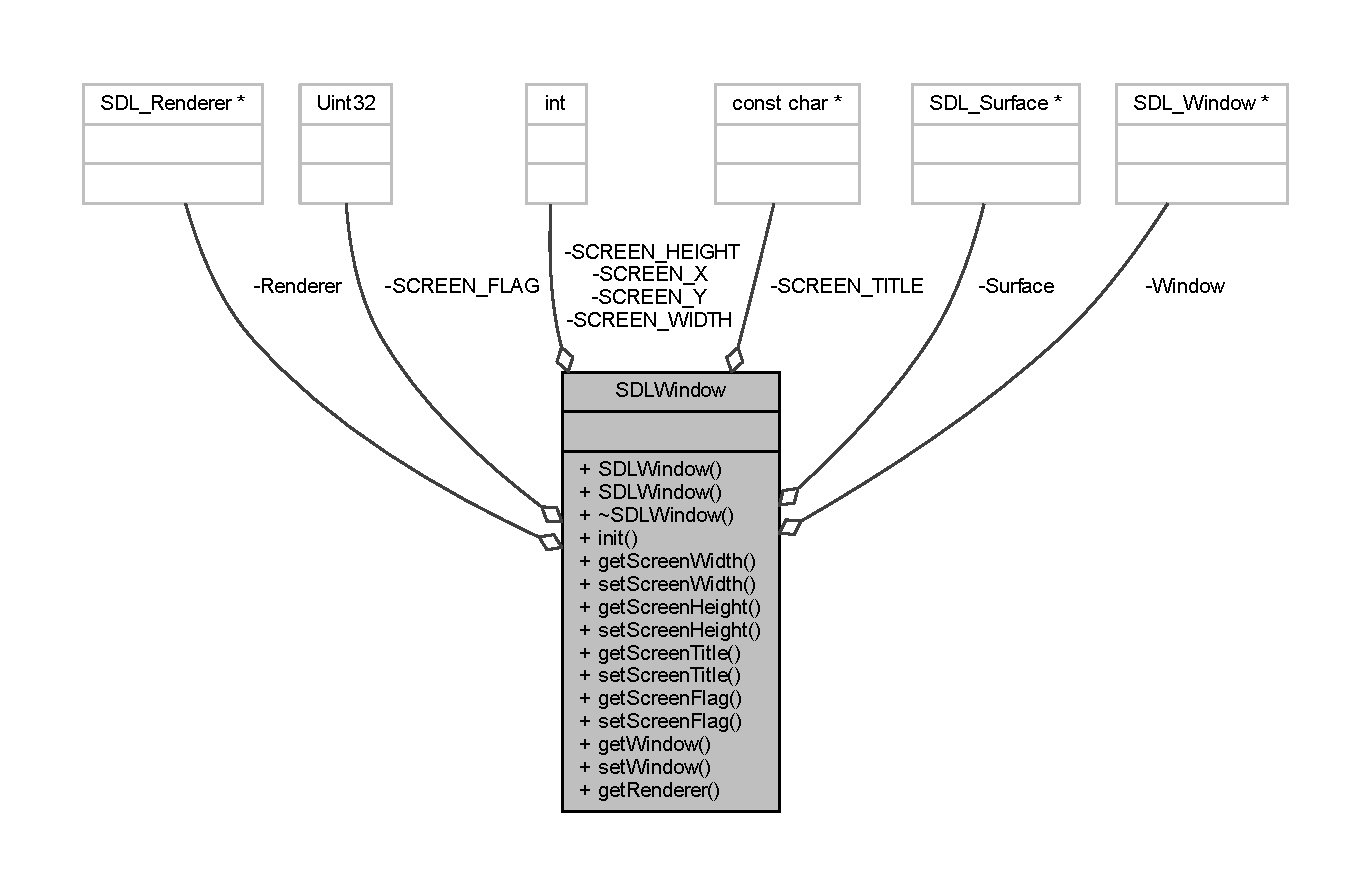
\includegraphics[width=350pt]{class_s_d_l_window__coll__graph}
\end{center}
\end{figure}
\subsection*{Public Member Functions}
\begin{DoxyCompactItemize}
\item 
\hyperlink{class_s_d_l_window_ab081329db76eaeaed1716c2e3bad50b2}{S\+D\+L\+Window} ()
\item 
\hyperlink{class_s_d_l_window_a9f42587fe7eeda9b87e060bf74891338}{S\+D\+L\+Window} (char $\ast$title, int x, int y, int width, int height, Uint32 flag)
\item 
\hyperlink{class_s_d_l_window_a7a0af0daec54970ff2262b67a6ece281}{$\sim$\+S\+D\+L\+Window} ()
\item 
bool \hyperlink{class_s_d_l_window_ad0f1f0b8510c97c1eeeffffe30707b0c}{init} ()
\item 
int \hyperlink{class_s_d_l_window_ad9bd55d793deb62b26932c5e1b8c1042}{get\+Screen\+Width} ()
\item 
void \hyperlink{class_s_d_l_window_a36930c7e4f3dee77c19283a3ede6287d}{set\+Screen\+Width} (int width)
\item 
int \hyperlink{class_s_d_l_window_ae3220fe9d6ef946c50713c7e4b72d637}{get\+Screen\+Height} ()
\item 
void \hyperlink{class_s_d_l_window_ae80e9b827e6c2138f1506841a60a072b}{set\+Screen\+Height} (int height)
\item 
const char $\ast$ \hyperlink{class_s_d_l_window_a7a21e853e2875a2a2324a59eefd04057}{get\+Screen\+Title} ()
\item 
void \hyperlink{class_s_d_l_window_a1be36c2e5e329d203e929d59f2d5c308}{set\+Screen\+Title} (const char $\ast$title)
\item 
Uint32 \hyperlink{class_s_d_l_window_adec65d41c9403d18cc23389a62f1897a}{get\+Screen\+Flag} ()
\item 
void \hyperlink{class_s_d_l_window_a032e69e9664f4cfdb3e27e82d3bab986}{set\+Screen\+Flag} (Uint32 flag)
\item 
S\+D\+L\+\_\+\+Window $\ast$ \hyperlink{class_s_d_l_window_a7b170e4afb9920aba42be65369cf98eb}{get\+Window} ()
\item 
void \hyperlink{class_s_d_l_window_ad14a7b1965115315210ba34b7239e598}{set\+Window} (const char $\ast$title, int x, int y, int width, int height, Uint32 flag)
\item 
S\+D\+L\+\_\+\+Renderer $\ast$ \hyperlink{class_s_d_l_window_a9a6d80f754ee6209be95d6c964dea85e}{get\+Renderer} ()
\end{DoxyCompactItemize}
\subsection*{Private Attributes}
\begin{DoxyCompactItemize}
\item 
S\+D\+L\+\_\+\+Window $\ast$ \hyperlink{class_s_d_l_window_aa95576b14f59ec62a9e7f6fb8c2f79cc}{Window}
\item 
S\+D\+L\+\_\+\+Surface $\ast$ \hyperlink{class_s_d_l_window_a7e7b7186d315e3294fb1761e1eb284ae}{Surface}
\item 
S\+D\+L\+\_\+\+Renderer $\ast$ \hyperlink{class_s_d_l_window_ae679402fd05b8eb3fd8680f1f036aaca}{Renderer}
\item 
const char $\ast$ \hyperlink{class_s_d_l_window_afeb1a7d48dde026d437babea6667ebee}{S\+C\+R\+E\+E\+N\+\_\+\+T\+I\+T\+LE}
\item 
int \hyperlink{class_s_d_l_window_ade54e8777a5e5017b139b4559c791634}{S\+C\+R\+E\+E\+N\+\_\+X}
\item 
int \hyperlink{class_s_d_l_window_abdb8d6136e9724e854c491cb9eef054d}{S\+C\+R\+E\+E\+N\+\_\+Y}
\item 
int \hyperlink{class_s_d_l_window_ab3faec77de829876613ea52176ef61e1}{S\+C\+R\+E\+E\+N\+\_\+\+W\+I\+D\+TH}
\item 
int \hyperlink{class_s_d_l_window_aed36cc4e541ecf78cda7e92f99a84d71}{S\+C\+R\+E\+E\+N\+\_\+\+H\+E\+I\+G\+HT}
\item 
Uint32 \hyperlink{class_s_d_l_window_a52d0a3b9ea7107e63476b24bc8a43397}{S\+C\+R\+E\+E\+N\+\_\+\+F\+L\+AG}
\end{DoxyCompactItemize}


\subsection{Detailed Description}
wrapper for the S\+DL window and renderer within the application 

Definition at line 9 of file S\+D\+L\+Window.\+h.



\subsection{Constructor \& Destructor Documentation}
\mbox{\Hypertarget{class_s_d_l_window_ab081329db76eaeaed1716c2e3bad50b2}\label{class_s_d_l_window_ab081329db76eaeaed1716c2e3bad50b2}} 
\index{S\+D\+L\+Window@{S\+D\+L\+Window}!S\+D\+L\+Window@{S\+D\+L\+Window}}
\index{S\+D\+L\+Window@{S\+D\+L\+Window}!S\+D\+L\+Window@{S\+D\+L\+Window}}
\subsubsection{\texorpdfstring{S\+D\+L\+Window()}{SDLWindow()}\hspace{0.1cm}{\footnotesize\ttfamily [1/2]}}
{\footnotesize\ttfamily S\+D\+L\+Window\+::\+S\+D\+L\+Window (\begin{DoxyParamCaption}{ }\end{DoxyParamCaption})}



Definition at line 3 of file S\+D\+L\+Window.\+cpp.


\begin{DoxyCode}
4 \{
5 
6 \}
\end{DoxyCode}
\mbox{\Hypertarget{class_s_d_l_window_a9f42587fe7eeda9b87e060bf74891338}\label{class_s_d_l_window_a9f42587fe7eeda9b87e060bf74891338}} 
\index{S\+D\+L\+Window@{S\+D\+L\+Window}!S\+D\+L\+Window@{S\+D\+L\+Window}}
\index{S\+D\+L\+Window@{S\+D\+L\+Window}!S\+D\+L\+Window@{S\+D\+L\+Window}}
\subsubsection{\texorpdfstring{S\+D\+L\+Window()}{SDLWindow()}\hspace{0.1cm}{\footnotesize\ttfamily [2/2]}}
{\footnotesize\ttfamily S\+D\+L\+Window\+::\+S\+D\+L\+Window (\begin{DoxyParamCaption}\item[{char $\ast$}]{title,  }\item[{int}]{x,  }\item[{int}]{y,  }\item[{int}]{width,  }\item[{int}]{height,  }\item[{Uint32}]{flag }\end{DoxyParamCaption})}



Definition at line 8 of file S\+D\+L\+Window.\+cpp.


\begin{DoxyCode}
8                                                                                  : 
      \hyperlink{class_s_d_l_window_ade54e8777a5e5017b139b4559c791634}{SCREEN\_X}(x), \hyperlink{class_s_d_l_window_abdb8d6136e9724e854c491cb9eef054d}{SCREEN\_Y}(y), \hyperlink{class_s_d_l_window_ab3faec77de829876613ea52176ef61e1}{SCREEN\_WIDTH}(width), 
      \hyperlink{class_s_d_l_window_aed36cc4e541ecf78cda7e92f99a84d71}{SCREEN\_HEIGHT}(height), \hyperlink{class_s_d_l_window_afeb1a7d48dde026d437babea6667ebee}{SCREEN\_TITLE}(title), \hyperlink{class_s_d_l_window_a52d0a3b9ea7107e63476b24bc8a43397}{SCREEN\_FLAG}(flag)
9 \{
10 
11 \}
\end{DoxyCode}
\mbox{\Hypertarget{class_s_d_l_window_a7a0af0daec54970ff2262b67a6ece281}\label{class_s_d_l_window_a7a0af0daec54970ff2262b67a6ece281}} 
\index{S\+D\+L\+Window@{S\+D\+L\+Window}!````~S\+D\+L\+Window@{$\sim$\+S\+D\+L\+Window}}
\index{````~S\+D\+L\+Window@{$\sim$\+S\+D\+L\+Window}!S\+D\+L\+Window@{S\+D\+L\+Window}}
\subsubsection{\texorpdfstring{$\sim$\+S\+D\+L\+Window()}{~SDLWindow()}}
{\footnotesize\ttfamily S\+D\+L\+Window\+::$\sim$\+S\+D\+L\+Window (\begin{DoxyParamCaption}{ }\end{DoxyParamCaption})}



Definition at line 13 of file S\+D\+L\+Window.\+cpp.



References Renderer, and Window.


\begin{DoxyCode}
14 \{
15     SDL\_DestroyRenderer(\hyperlink{class_s_d_l_window_ae679402fd05b8eb3fd8680f1f036aaca}{Renderer});
16     SDL\_DestroyWindow(\hyperlink{class_s_d_l_window_aa95576b14f59ec62a9e7f6fb8c2f79cc}{Window});
17     \hyperlink{class_s_d_l_window_aa95576b14f59ec62a9e7f6fb8c2f79cc}{Window} = NULL;
18     \hyperlink{class_s_d_l_window_ae679402fd05b8eb3fd8680f1f036aaca}{Renderer} = NULL;
19     IMG\_Quit();
20     SDL\_Quit();
21 \}
\end{DoxyCode}


\subsection{Member Function Documentation}
\mbox{\Hypertarget{class_s_d_l_window_a9a6d80f754ee6209be95d6c964dea85e}\label{class_s_d_l_window_a9a6d80f754ee6209be95d6c964dea85e}} 
\index{S\+D\+L\+Window@{S\+D\+L\+Window}!get\+Renderer@{get\+Renderer}}
\index{get\+Renderer@{get\+Renderer}!S\+D\+L\+Window@{S\+D\+L\+Window}}
\subsubsection{\texorpdfstring{get\+Renderer()}{getRenderer()}}
{\footnotesize\ttfamily S\+D\+L\+\_\+\+Renderer $\ast$ S\+D\+L\+Window\+::get\+Renderer (\begin{DoxyParamCaption}{ }\end{DoxyParamCaption})}



Definition at line 73 of file S\+D\+L\+Window.\+cpp.



References Renderer.



Referenced by main().


\begin{DoxyCode}
74 \{
75     \textcolor{keywordflow}{return} \hyperlink{class_s_d_l_window_ae679402fd05b8eb3fd8680f1f036aaca}{Renderer};
76 \}
\end{DoxyCode}
\mbox{\Hypertarget{class_s_d_l_window_adec65d41c9403d18cc23389a62f1897a}\label{class_s_d_l_window_adec65d41c9403d18cc23389a62f1897a}} 
\index{S\+D\+L\+Window@{S\+D\+L\+Window}!get\+Screen\+Flag@{get\+Screen\+Flag}}
\index{get\+Screen\+Flag@{get\+Screen\+Flag}!S\+D\+L\+Window@{S\+D\+L\+Window}}
\subsubsection{\texorpdfstring{get\+Screen\+Flag()}{getScreenFlag()}}
{\footnotesize\ttfamily Uint32 S\+D\+L\+Window\+::get\+Screen\+Flag (\begin{DoxyParamCaption}{ }\end{DoxyParamCaption})}



Definition at line 63 of file S\+D\+L\+Window.\+cpp.



References S\+C\+R\+E\+E\+N\+\_\+\+F\+L\+AG.


\begin{DoxyCode}
64 \{
65     \textcolor{keywordflow}{return} \hyperlink{class_s_d_l_window_a52d0a3b9ea7107e63476b24bc8a43397}{SCREEN\_FLAG};
66 \}
\end{DoxyCode}
\mbox{\Hypertarget{class_s_d_l_window_ae3220fe9d6ef946c50713c7e4b72d637}\label{class_s_d_l_window_ae3220fe9d6ef946c50713c7e4b72d637}} 
\index{S\+D\+L\+Window@{S\+D\+L\+Window}!get\+Screen\+Height@{get\+Screen\+Height}}
\index{get\+Screen\+Height@{get\+Screen\+Height}!S\+D\+L\+Window@{S\+D\+L\+Window}}
\subsubsection{\texorpdfstring{get\+Screen\+Height()}{getScreenHeight()}}
{\footnotesize\ttfamily int S\+D\+L\+Window\+::get\+Screen\+Height (\begin{DoxyParamCaption}{ }\end{DoxyParamCaption})}



Definition at line 33 of file S\+D\+L\+Window.\+cpp.



References S\+C\+R\+E\+E\+N\+\_\+\+H\+E\+I\+G\+HT.



Referenced by main().


\begin{DoxyCode}
34 \{
35     \textcolor{keywordflow}{return} \hyperlink{class_s_d_l_window_aed36cc4e541ecf78cda7e92f99a84d71}{SCREEN\_HEIGHT};
36 \}
\end{DoxyCode}
\mbox{\Hypertarget{class_s_d_l_window_a7a21e853e2875a2a2324a59eefd04057}\label{class_s_d_l_window_a7a21e853e2875a2a2324a59eefd04057}} 
\index{S\+D\+L\+Window@{S\+D\+L\+Window}!get\+Screen\+Title@{get\+Screen\+Title}}
\index{get\+Screen\+Title@{get\+Screen\+Title}!S\+D\+L\+Window@{S\+D\+L\+Window}}
\subsubsection{\texorpdfstring{get\+Screen\+Title()}{getScreenTitle()}}
{\footnotesize\ttfamily const char $\ast$ S\+D\+L\+Window\+::get\+Screen\+Title (\begin{DoxyParamCaption}{ }\end{DoxyParamCaption})}



Definition at line 53 of file S\+D\+L\+Window.\+cpp.



References S\+C\+R\+E\+E\+N\+\_\+\+T\+I\+T\+LE.


\begin{DoxyCode}
54 \{
55     \textcolor{keywordflow}{return} \hyperlink{class_s_d_l_window_afeb1a7d48dde026d437babea6667ebee}{SCREEN\_TITLE};
56 \}
\end{DoxyCode}
\mbox{\Hypertarget{class_s_d_l_window_ad9bd55d793deb62b26932c5e1b8c1042}\label{class_s_d_l_window_ad9bd55d793deb62b26932c5e1b8c1042}} 
\index{S\+D\+L\+Window@{S\+D\+L\+Window}!get\+Screen\+Width@{get\+Screen\+Width}}
\index{get\+Screen\+Width@{get\+Screen\+Width}!S\+D\+L\+Window@{S\+D\+L\+Window}}
\subsubsection{\texorpdfstring{get\+Screen\+Width()}{getScreenWidth()}}
{\footnotesize\ttfamily int S\+D\+L\+Window\+::get\+Screen\+Width (\begin{DoxyParamCaption}{ }\end{DoxyParamCaption})}



Definition at line 43 of file S\+D\+L\+Window.\+cpp.



References S\+C\+R\+E\+E\+N\+\_\+\+W\+I\+D\+TH.



Referenced by main().


\begin{DoxyCode}
44 \{
45     \textcolor{keywordflow}{return} \hyperlink{class_s_d_l_window_ab3faec77de829876613ea52176ef61e1}{SCREEN\_WIDTH};
46 \}
\end{DoxyCode}
\mbox{\Hypertarget{class_s_d_l_window_a7b170e4afb9920aba42be65369cf98eb}\label{class_s_d_l_window_a7b170e4afb9920aba42be65369cf98eb}} 
\index{S\+D\+L\+Window@{S\+D\+L\+Window}!get\+Window@{get\+Window}}
\index{get\+Window@{get\+Window}!S\+D\+L\+Window@{S\+D\+L\+Window}}
\subsubsection{\texorpdfstring{get\+Window()}{getWindow()}}
{\footnotesize\ttfamily S\+D\+L\+\_\+\+Window $\ast$ S\+D\+L\+Window\+::get\+Window (\begin{DoxyParamCaption}{ }\end{DoxyParamCaption})}



Definition at line 28 of file S\+D\+L\+Window.\+cpp.



References Window.


\begin{DoxyCode}
29 \{
30     \textcolor{keywordflow}{return} \hyperlink{class_s_d_l_window_aa95576b14f59ec62a9e7f6fb8c2f79cc}{Window};
31 \}
\end{DoxyCode}
\mbox{\Hypertarget{class_s_d_l_window_ad0f1f0b8510c97c1eeeffffe30707b0c}\label{class_s_d_l_window_ad0f1f0b8510c97c1eeeffffe30707b0c}} 
\index{S\+D\+L\+Window@{S\+D\+L\+Window}!init@{init}}
\index{init@{init}!S\+D\+L\+Window@{S\+D\+L\+Window}}
\subsubsection{\texorpdfstring{init()}{init()}}
{\footnotesize\ttfamily bool S\+D\+L\+Window\+::init (\begin{DoxyParamCaption}{ }\end{DoxyParamCaption})}



Definition at line 78 of file S\+D\+L\+Window.\+cpp.



References Renderer, S\+C\+R\+E\+E\+N\+\_\+\+F\+L\+AG, S\+C\+R\+E\+E\+N\+\_\+\+H\+E\+I\+G\+HT, S\+C\+R\+E\+E\+N\+\_\+\+T\+I\+T\+LE, S\+C\+R\+E\+E\+N\+\_\+\+W\+I\+D\+TH, S\+C\+R\+E\+E\+N\+\_\+X, S\+C\+R\+E\+E\+N\+\_\+Y, set\+Window(), and Window.



Referenced by main().


\begin{DoxyCode}
79 \{
80     \textcolor{keywordtype}{bool} success = \textcolor{keyword}{true};
81 
82     \textcolor{keywordflow}{if} (SDL\_Init(SDL\_INIT\_VIDEO) < 0)
83     \{
84         printf(\textcolor{stringliteral}{"SDL could not initialize! SDL\_Error: %s\(\backslash\)n"}, SDL\_GetError());
85         success = \textcolor{keyword}{false};
86     \}
87     \textcolor{keywordflow}{else}
88     \{
89         \textcolor{comment}{//Set texture filtering to linear}
90         \textcolor{keywordflow}{if} (!SDL\_SetHint(SDL\_HINT\_RENDER\_SCALE\_QUALITY, \textcolor{stringliteral}{"1"}))
91         \{
92             printf(\textcolor{stringliteral}{"Warning: Linear texture filtering not enabled!"});
93         \}
94 
95         \hyperlink{class_s_d_l_window_ad14a7b1965115315210ba34b7239e598}{setWindow}(\hyperlink{class_s_d_l_window_afeb1a7d48dde026d437babea6667ebee}{SCREEN\_TITLE}, \hyperlink{class_s_d_l_window_ade54e8777a5e5017b139b4559c791634}{SCREEN\_X}, \hyperlink{class_s_d_l_window_abdb8d6136e9724e854c491cb9eef054d}{SCREEN\_Y}, 
      \hyperlink{class_s_d_l_window_ab3faec77de829876613ea52176ef61e1}{SCREEN\_WIDTH}, \hyperlink{class_s_d_l_window_aed36cc4e541ecf78cda7e92f99a84d71}{SCREEN\_HEIGHT}, \hyperlink{class_s_d_l_window_a52d0a3b9ea7107e63476b24bc8a43397}{SCREEN\_FLAG});
96         \textcolor{keywordflow}{if} (\hyperlink{class_s_d_l_window_aa95576b14f59ec62a9e7f6fb8c2f79cc}{Window} == NULL)
97         \{
98             printf(\textcolor{stringliteral}{"Window could not be created! SDL\_Error: %s\(\backslash\)n"}, SDL\_GetError());
99             success = \textcolor{keyword}{false};
100         \}
101         \textcolor{keywordflow}{else}
102         \{
103             \hyperlink{class_s_d_l_window_ae679402fd05b8eb3fd8680f1f036aaca}{Renderer} = SDL\_CreateRenderer(\hyperlink{class_s_d_l_window_aa95576b14f59ec62a9e7f6fb8c2f79cc}{Window}, -1, SDL\_RENDERER\_ACCELERATED | 
      SDL\_RENDERER\_PRESENTVSYNC);
104             \textcolor{keywordflow}{if} (\hyperlink{class_s_d_l_window_ae679402fd05b8eb3fd8680f1f036aaca}{Renderer} == NULL)
105             \{
106                 printf(\textcolor{stringliteral}{"Renderer could not be created! SDL\_Error: %s\(\backslash\)n"}, SDL\_GetError());
107                 success = \textcolor{keyword}{false};
108             \}
109             \textcolor{keywordflow}{else}
110             \{
111                 SDL\_SetRenderDrawColor(\hyperlink{class_s_d_l_window_ae679402fd05b8eb3fd8680f1f036aaca}{Renderer}, 0xFF, 0xFF, 0xFF, 0xFF);
112 
113                 \textcolor{keywordtype}{int} imgFlags = IMG\_INIT\_PNG;
114                 \textcolor{keywordflow}{if} (!(IMG\_Init(imgFlags) & imgFlags))
115                 \{
116                     printf(\textcolor{stringliteral}{"SDL\_image could not initialize! SDL\_image Error: %s\(\backslash\)n"}, IMG\_GetError());
117                     success = \textcolor{keyword}{false};
118                 \}
119 
120                 \textcolor{keywordflow}{if} (TTF\_Init() == -1)
121                 \{
122                     printf(\textcolor{stringliteral}{"SDL\_ttf could not initialize! SDL\_ttf Error: %s\(\backslash\)n"}, TTF\_GetError());
123                     success = \textcolor{keyword}{false};
124                 \}
125             \}
126         \}
127     \}
128 
129     \textcolor{keywordflow}{return} success;
130 \}
\end{DoxyCode}
\mbox{\Hypertarget{class_s_d_l_window_a032e69e9664f4cfdb3e27e82d3bab986}\label{class_s_d_l_window_a032e69e9664f4cfdb3e27e82d3bab986}} 
\index{S\+D\+L\+Window@{S\+D\+L\+Window}!set\+Screen\+Flag@{set\+Screen\+Flag}}
\index{set\+Screen\+Flag@{set\+Screen\+Flag}!S\+D\+L\+Window@{S\+D\+L\+Window}}
\subsubsection{\texorpdfstring{set\+Screen\+Flag()}{setScreenFlag()}}
{\footnotesize\ttfamily void S\+D\+L\+Window\+::set\+Screen\+Flag (\begin{DoxyParamCaption}\item[{Uint32}]{flag }\end{DoxyParamCaption})}



Definition at line 68 of file S\+D\+L\+Window.\+cpp.



References S\+C\+R\+E\+E\+N\+\_\+\+F\+L\+AG.


\begin{DoxyCode}
69 \{
70     \hyperlink{class_s_d_l_window_a52d0a3b9ea7107e63476b24bc8a43397}{SCREEN\_FLAG} = flag;
71 \}
\end{DoxyCode}
\mbox{\Hypertarget{class_s_d_l_window_ae80e9b827e6c2138f1506841a60a072b}\label{class_s_d_l_window_ae80e9b827e6c2138f1506841a60a072b}} 
\index{S\+D\+L\+Window@{S\+D\+L\+Window}!set\+Screen\+Height@{set\+Screen\+Height}}
\index{set\+Screen\+Height@{set\+Screen\+Height}!S\+D\+L\+Window@{S\+D\+L\+Window}}
\subsubsection{\texorpdfstring{set\+Screen\+Height()}{setScreenHeight()}}
{\footnotesize\ttfamily void S\+D\+L\+Window\+::set\+Screen\+Height (\begin{DoxyParamCaption}\item[{int}]{height }\end{DoxyParamCaption})}



Definition at line 38 of file S\+D\+L\+Window.\+cpp.



References S\+C\+R\+E\+E\+N\+\_\+\+H\+E\+I\+G\+HT.


\begin{DoxyCode}
39 \{
40     \hyperlink{class_s_d_l_window_aed36cc4e541ecf78cda7e92f99a84d71}{SCREEN\_HEIGHT} = height;
41 \}
\end{DoxyCode}
\mbox{\Hypertarget{class_s_d_l_window_a1be36c2e5e329d203e929d59f2d5c308}\label{class_s_d_l_window_a1be36c2e5e329d203e929d59f2d5c308}} 
\index{S\+D\+L\+Window@{S\+D\+L\+Window}!set\+Screen\+Title@{set\+Screen\+Title}}
\index{set\+Screen\+Title@{set\+Screen\+Title}!S\+D\+L\+Window@{S\+D\+L\+Window}}
\subsubsection{\texorpdfstring{set\+Screen\+Title()}{setScreenTitle()}}
{\footnotesize\ttfamily void S\+D\+L\+Window\+::set\+Screen\+Title (\begin{DoxyParamCaption}\item[{const char $\ast$}]{title }\end{DoxyParamCaption})}



Definition at line 58 of file S\+D\+L\+Window.\+cpp.



References S\+C\+R\+E\+E\+N\+\_\+\+T\+I\+T\+LE.


\begin{DoxyCode}
59 \{
60     \hyperlink{class_s_d_l_window_afeb1a7d48dde026d437babea6667ebee}{SCREEN\_TITLE} = title;
61 \}
\end{DoxyCode}
\mbox{\Hypertarget{class_s_d_l_window_a36930c7e4f3dee77c19283a3ede6287d}\label{class_s_d_l_window_a36930c7e4f3dee77c19283a3ede6287d}} 
\index{S\+D\+L\+Window@{S\+D\+L\+Window}!set\+Screen\+Width@{set\+Screen\+Width}}
\index{set\+Screen\+Width@{set\+Screen\+Width}!S\+D\+L\+Window@{S\+D\+L\+Window}}
\subsubsection{\texorpdfstring{set\+Screen\+Width()}{setScreenWidth()}}
{\footnotesize\ttfamily void S\+D\+L\+Window\+::set\+Screen\+Width (\begin{DoxyParamCaption}\item[{int}]{width }\end{DoxyParamCaption})}



Definition at line 48 of file S\+D\+L\+Window.\+cpp.



References S\+C\+R\+E\+E\+N\+\_\+\+W\+I\+D\+TH.


\begin{DoxyCode}
49 \{
50     \hyperlink{class_s_d_l_window_ab3faec77de829876613ea52176ef61e1}{SCREEN\_WIDTH} = width;
51 \}
\end{DoxyCode}
\mbox{\Hypertarget{class_s_d_l_window_ad14a7b1965115315210ba34b7239e598}\label{class_s_d_l_window_ad14a7b1965115315210ba34b7239e598}} 
\index{S\+D\+L\+Window@{S\+D\+L\+Window}!set\+Window@{set\+Window}}
\index{set\+Window@{set\+Window}!S\+D\+L\+Window@{S\+D\+L\+Window}}
\subsubsection{\texorpdfstring{set\+Window()}{setWindow()}}
{\footnotesize\ttfamily void S\+D\+L\+Window\+::set\+Window (\begin{DoxyParamCaption}\item[{const char $\ast$}]{title,  }\item[{int}]{x,  }\item[{int}]{y,  }\item[{int}]{width,  }\item[{int}]{height,  }\item[{Uint32}]{flag }\end{DoxyParamCaption})}



Definition at line 23 of file S\+D\+L\+Window.\+cpp.



References Window.



Referenced by init().


\begin{DoxyCode}
24 \{
25     \hyperlink{class_s_d_l_window_aa95576b14f59ec62a9e7f6fb8c2f79cc}{Window} = SDL\_CreateWindow(title, x, y, width, height, flag);
26 \}
\end{DoxyCode}


\subsection{Member Data Documentation}
\mbox{\Hypertarget{class_s_d_l_window_ae679402fd05b8eb3fd8680f1f036aaca}\label{class_s_d_l_window_ae679402fd05b8eb3fd8680f1f036aaca}} 
\index{S\+D\+L\+Window@{S\+D\+L\+Window}!Renderer@{Renderer}}
\index{Renderer@{Renderer}!S\+D\+L\+Window@{S\+D\+L\+Window}}
\subsubsection{\texorpdfstring{Renderer}{Renderer}}
{\footnotesize\ttfamily S\+D\+L\+\_\+\+Renderer$\ast$ S\+D\+L\+Window\+::\+Renderer\hspace{0.3cm}{\ttfamily [private]}}



Definition at line 37 of file S\+D\+L\+Window.\+h.



Referenced by get\+Renderer(), init(), and $\sim$\+S\+D\+L\+Window().

\mbox{\Hypertarget{class_s_d_l_window_a52d0a3b9ea7107e63476b24bc8a43397}\label{class_s_d_l_window_a52d0a3b9ea7107e63476b24bc8a43397}} 
\index{S\+D\+L\+Window@{S\+D\+L\+Window}!S\+C\+R\+E\+E\+N\+\_\+\+F\+L\+AG@{S\+C\+R\+E\+E\+N\+\_\+\+F\+L\+AG}}
\index{S\+C\+R\+E\+E\+N\+\_\+\+F\+L\+AG@{S\+C\+R\+E\+E\+N\+\_\+\+F\+L\+AG}!S\+D\+L\+Window@{S\+D\+L\+Window}}
\subsubsection{\texorpdfstring{S\+C\+R\+E\+E\+N\+\_\+\+F\+L\+AG}{SCREEN\_FLAG}}
{\footnotesize\ttfamily Uint32 S\+D\+L\+Window\+::\+S\+C\+R\+E\+E\+N\+\_\+\+F\+L\+AG\hspace{0.3cm}{\ttfamily [private]}}



Definition at line 44 of file S\+D\+L\+Window.\+h.



Referenced by get\+Screen\+Flag(), init(), and set\+Screen\+Flag().

\mbox{\Hypertarget{class_s_d_l_window_aed36cc4e541ecf78cda7e92f99a84d71}\label{class_s_d_l_window_aed36cc4e541ecf78cda7e92f99a84d71}} 
\index{S\+D\+L\+Window@{S\+D\+L\+Window}!S\+C\+R\+E\+E\+N\+\_\+\+H\+E\+I\+G\+HT@{S\+C\+R\+E\+E\+N\+\_\+\+H\+E\+I\+G\+HT}}
\index{S\+C\+R\+E\+E\+N\+\_\+\+H\+E\+I\+G\+HT@{S\+C\+R\+E\+E\+N\+\_\+\+H\+E\+I\+G\+HT}!S\+D\+L\+Window@{S\+D\+L\+Window}}
\subsubsection{\texorpdfstring{S\+C\+R\+E\+E\+N\+\_\+\+H\+E\+I\+G\+HT}{SCREEN\_HEIGHT}}
{\footnotesize\ttfamily int S\+D\+L\+Window\+::\+S\+C\+R\+E\+E\+N\+\_\+\+H\+E\+I\+G\+HT\hspace{0.3cm}{\ttfamily [private]}}



Definition at line 43 of file S\+D\+L\+Window.\+h.



Referenced by get\+Screen\+Height(), init(), and set\+Screen\+Height().

\mbox{\Hypertarget{class_s_d_l_window_afeb1a7d48dde026d437babea6667ebee}\label{class_s_d_l_window_afeb1a7d48dde026d437babea6667ebee}} 
\index{S\+D\+L\+Window@{S\+D\+L\+Window}!S\+C\+R\+E\+E\+N\+\_\+\+T\+I\+T\+LE@{S\+C\+R\+E\+E\+N\+\_\+\+T\+I\+T\+LE}}
\index{S\+C\+R\+E\+E\+N\+\_\+\+T\+I\+T\+LE@{S\+C\+R\+E\+E\+N\+\_\+\+T\+I\+T\+LE}!S\+D\+L\+Window@{S\+D\+L\+Window}}
\subsubsection{\texorpdfstring{S\+C\+R\+E\+E\+N\+\_\+\+T\+I\+T\+LE}{SCREEN\_TITLE}}
{\footnotesize\ttfamily const char$\ast$ S\+D\+L\+Window\+::\+S\+C\+R\+E\+E\+N\+\_\+\+T\+I\+T\+LE\hspace{0.3cm}{\ttfamily [private]}}



Definition at line 39 of file S\+D\+L\+Window.\+h.



Referenced by get\+Screen\+Title(), init(), and set\+Screen\+Title().

\mbox{\Hypertarget{class_s_d_l_window_ab3faec77de829876613ea52176ef61e1}\label{class_s_d_l_window_ab3faec77de829876613ea52176ef61e1}} 
\index{S\+D\+L\+Window@{S\+D\+L\+Window}!S\+C\+R\+E\+E\+N\+\_\+\+W\+I\+D\+TH@{S\+C\+R\+E\+E\+N\+\_\+\+W\+I\+D\+TH}}
\index{S\+C\+R\+E\+E\+N\+\_\+\+W\+I\+D\+TH@{S\+C\+R\+E\+E\+N\+\_\+\+W\+I\+D\+TH}!S\+D\+L\+Window@{S\+D\+L\+Window}}
\subsubsection{\texorpdfstring{S\+C\+R\+E\+E\+N\+\_\+\+W\+I\+D\+TH}{SCREEN\_WIDTH}}
{\footnotesize\ttfamily int S\+D\+L\+Window\+::\+S\+C\+R\+E\+E\+N\+\_\+\+W\+I\+D\+TH\hspace{0.3cm}{\ttfamily [private]}}



Definition at line 42 of file S\+D\+L\+Window.\+h.



Referenced by get\+Screen\+Width(), init(), and set\+Screen\+Width().

\mbox{\Hypertarget{class_s_d_l_window_ade54e8777a5e5017b139b4559c791634}\label{class_s_d_l_window_ade54e8777a5e5017b139b4559c791634}} 
\index{S\+D\+L\+Window@{S\+D\+L\+Window}!S\+C\+R\+E\+E\+N\+\_\+X@{S\+C\+R\+E\+E\+N\+\_\+X}}
\index{S\+C\+R\+E\+E\+N\+\_\+X@{S\+C\+R\+E\+E\+N\+\_\+X}!S\+D\+L\+Window@{S\+D\+L\+Window}}
\subsubsection{\texorpdfstring{S\+C\+R\+E\+E\+N\+\_\+X}{SCREEN\_X}}
{\footnotesize\ttfamily int S\+D\+L\+Window\+::\+S\+C\+R\+E\+E\+N\+\_\+X\hspace{0.3cm}{\ttfamily [private]}}



Definition at line 40 of file S\+D\+L\+Window.\+h.



Referenced by init().

\mbox{\Hypertarget{class_s_d_l_window_abdb8d6136e9724e854c491cb9eef054d}\label{class_s_d_l_window_abdb8d6136e9724e854c491cb9eef054d}} 
\index{S\+D\+L\+Window@{S\+D\+L\+Window}!S\+C\+R\+E\+E\+N\+\_\+Y@{S\+C\+R\+E\+E\+N\+\_\+Y}}
\index{S\+C\+R\+E\+E\+N\+\_\+Y@{S\+C\+R\+E\+E\+N\+\_\+Y}!S\+D\+L\+Window@{S\+D\+L\+Window}}
\subsubsection{\texorpdfstring{S\+C\+R\+E\+E\+N\+\_\+Y}{SCREEN\_Y}}
{\footnotesize\ttfamily int S\+D\+L\+Window\+::\+S\+C\+R\+E\+E\+N\+\_\+Y\hspace{0.3cm}{\ttfamily [private]}}



Definition at line 41 of file S\+D\+L\+Window.\+h.



Referenced by init().

\mbox{\Hypertarget{class_s_d_l_window_a7e7b7186d315e3294fb1761e1eb284ae}\label{class_s_d_l_window_a7e7b7186d315e3294fb1761e1eb284ae}} 
\index{S\+D\+L\+Window@{S\+D\+L\+Window}!Surface@{Surface}}
\index{Surface@{Surface}!S\+D\+L\+Window@{S\+D\+L\+Window}}
\subsubsection{\texorpdfstring{Surface}{Surface}}
{\footnotesize\ttfamily S\+D\+L\+\_\+\+Surface$\ast$ S\+D\+L\+Window\+::\+Surface\hspace{0.3cm}{\ttfamily [private]}}



Definition at line 36 of file S\+D\+L\+Window.\+h.

\mbox{\Hypertarget{class_s_d_l_window_aa95576b14f59ec62a9e7f6fb8c2f79cc}\label{class_s_d_l_window_aa95576b14f59ec62a9e7f6fb8c2f79cc}} 
\index{S\+D\+L\+Window@{S\+D\+L\+Window}!Window@{Window}}
\index{Window@{Window}!S\+D\+L\+Window@{S\+D\+L\+Window}}
\subsubsection{\texorpdfstring{Window}{Window}}
{\footnotesize\ttfamily S\+D\+L\+\_\+\+Window$\ast$ S\+D\+L\+Window\+::\+Window\hspace{0.3cm}{\ttfamily [private]}}



Definition at line 35 of file S\+D\+L\+Window.\+h.



Referenced by get\+Window(), init(), set\+Window(), and $\sim$\+S\+D\+L\+Window().



The documentation for this class was generated from the following files\+:\begin{DoxyCompactItemize}
\item 
C\+:/\+Users/\+Kyle Tuckey/\+Documents/\+Final Year Project/\+Social\+\_\+\+N\+P\+C\+S/\+Social\+\_\+\+N\+P\+C\+S/\hyperlink{_s_d_l_window_8h}{S\+D\+L\+Window.\+h}\item 
C\+:/\+Users/\+Kyle Tuckey/\+Documents/\+Final Year Project/\+Social\+\_\+\+N\+P\+C\+S/\+Social\+\_\+\+N\+P\+C\+S/\hyperlink{_s_d_l_window_8cpp}{S\+D\+L\+Window.\+cpp}\end{DoxyCompactItemize}

\hypertarget{class_sprite}{}\section{Sprite Class Reference}
\label{class_sprite}\index{Sprite@{Sprite}}


{\ttfamily \#include $<$Sprite.\+h$>$}



Inheritance diagram for Sprite\+:\nopagebreak
\begin{figure}[H]
\begin{center}
\leavevmode
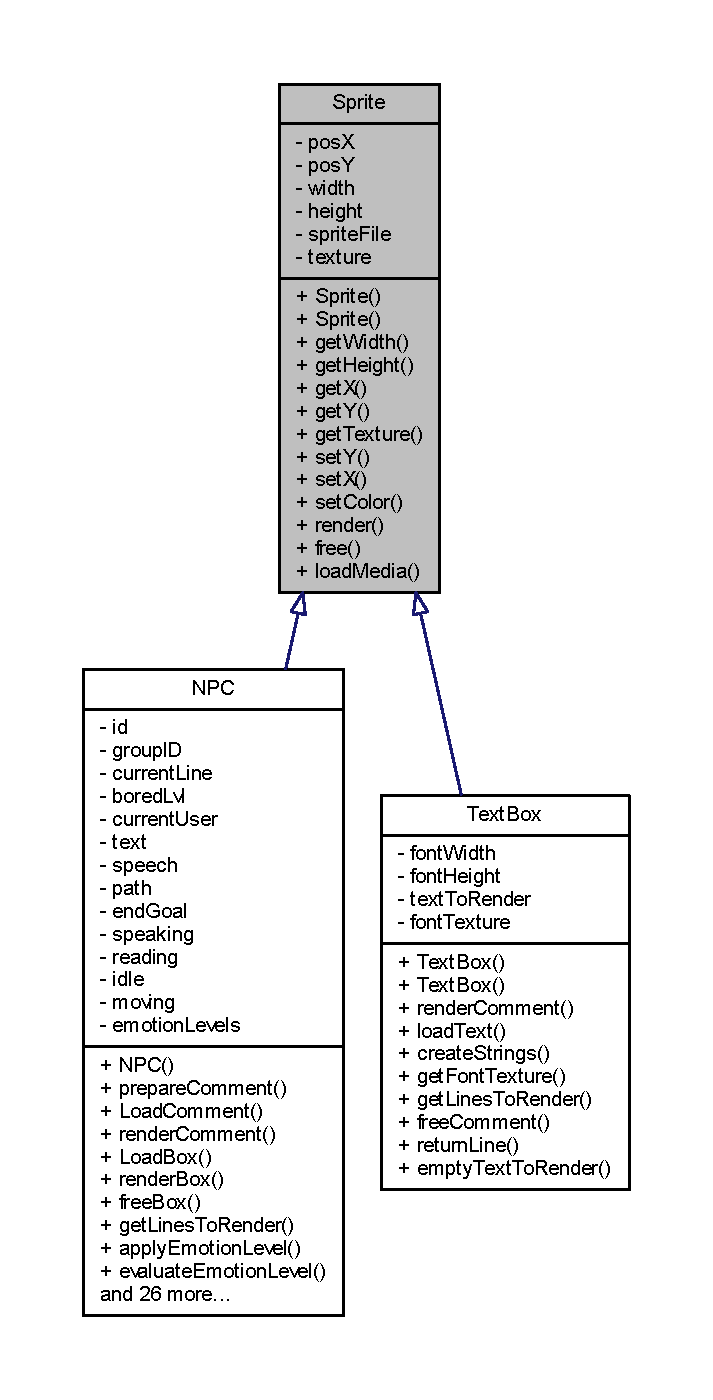
\includegraphics[height=550pt]{class_sprite__inherit__graph}
\end{center}
\end{figure}


Collaboration diagram for Sprite\+:\nopagebreak
\begin{figure}[H]
\begin{center}
\leavevmode
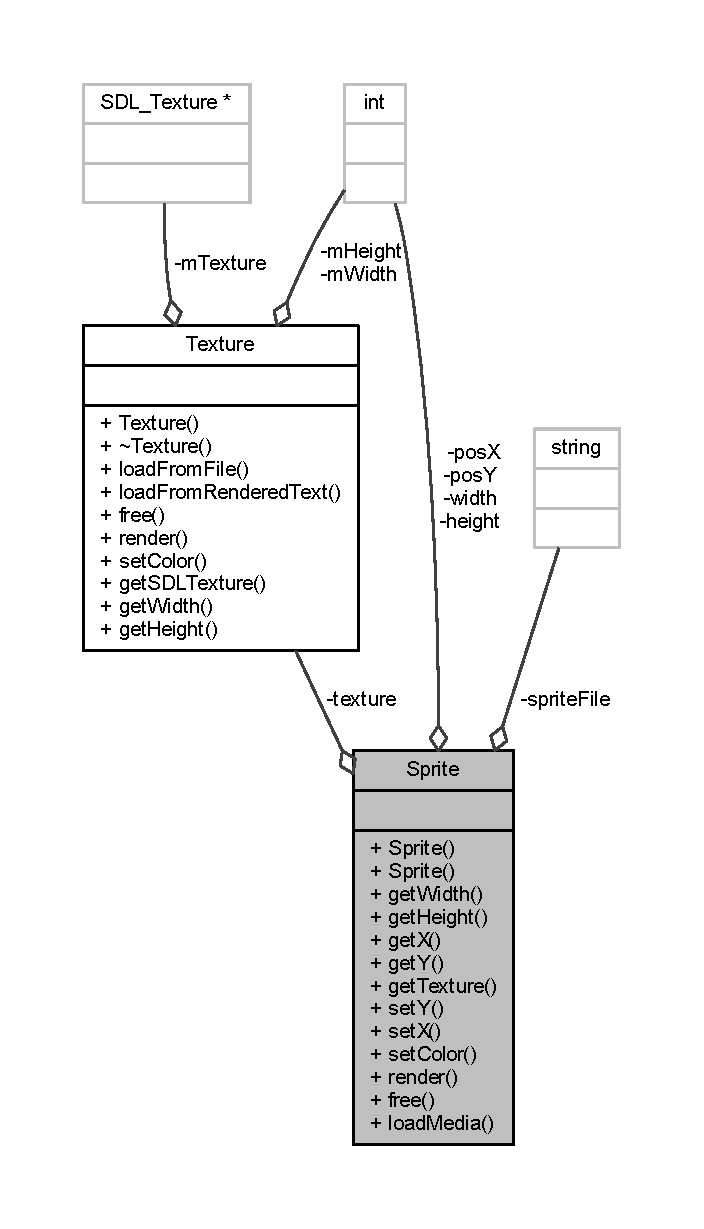
\includegraphics[height=550pt]{class_sprite__coll__graph}
\end{center}
\end{figure}
\subsection*{Public Member Functions}
\begin{DoxyCompactItemize}
\item 
\hyperlink{class_sprite_a12cba3ac1868418add3c4d95ce87e615}{Sprite} ()
\item 
\hyperlink{class_sprite_a9e4b47480afc64a0969d2b9014af02cc}{Sprite} (std\+::string file\+Name, S\+D\+L\+\_\+\+Renderer $\ast$renderer, int x=0, int y=0)
\item 
int \hyperlink{class_sprite_aba3d4752461ec679fbf5de7ec4c34f61}{get\+Width} ()
\item 
int \hyperlink{class_sprite_a67b67082cfda90103d2d9eefea04cc4b}{get\+Height} ()
\item 
int \hyperlink{class_sprite_a03d6c82bddfd3d164ce8997482c57c85}{getX} ()
\item 
int \hyperlink{class_sprite_a53ea8b27bcd0dab0627a2dceab2b9d98}{getY} ()
\item 
\hyperlink{class_texture}{Texture} \hyperlink{class_sprite_a95126cbe568a388a5b1092dee95716d0}{get\+Texture} ()
\item 
void \hyperlink{class_sprite_afe7d6d636fc460358c40a403af259d0e}{setY} (int y)
\item 
void \hyperlink{class_sprite_ae21322c28b8719af996990fafa920762}{setX} (int x)
\item 
void \hyperlink{class_sprite_a1ca0939610f24386a4eecb8e91688c65}{set\+Color} (int r, int g, int b)
\item 
void \hyperlink{class_sprite_a72231a3cc5414b94ab6bfcbddc3b327c}{render} (S\+D\+L\+\_\+\+Renderer $\ast$renderer)
\item 
void \hyperlink{class_sprite_abce3359b4f055bac7384038046ed9ead}{free} ()
\item 
bool \hyperlink{class_sprite_adab722e01e4d3e197f52ecad6ac8d70a}{load\+Media} (S\+D\+L\+\_\+\+Renderer $\ast$renderer)
\end{DoxyCompactItemize}
\subsection*{Private Attributes}
\begin{DoxyCompactItemize}
\item 
int \hyperlink{class_sprite_a0af496e3e6540f1f1321913a741a737a}{posX}
\item 
int \hyperlink{class_sprite_a1ef80a5eff9d5b0bb90ae355daf09efe}{posY}
\item 
int \hyperlink{class_sprite_a0a3364944c5e361fc9e7ae406224d682}{width}
\item 
int \hyperlink{class_sprite_a1f07c8f2080c193759aec0e13503d7ab}{height}
\item 
std\+::string \hyperlink{class_sprite_a595ffe434aadbc94b9abd272c0356c9d}{sprite\+File}
\item 
\hyperlink{class_texture}{Texture} \hyperlink{class_sprite_aa4978b284ebaae7225869d238dcb32cb}{texture}
\end{DoxyCompactItemize}


\subsection{Detailed Description}
Base sprite class, all graphical sprites will inherit this class 

Definition at line 7 of file Sprite.\+h.



\subsection{Constructor \& Destructor Documentation}
\mbox{\Hypertarget{class_sprite_a12cba3ac1868418add3c4d95ce87e615}\label{class_sprite_a12cba3ac1868418add3c4d95ce87e615}} 
\index{Sprite@{Sprite}!Sprite@{Sprite}}
\index{Sprite@{Sprite}!Sprite@{Sprite}}
\subsubsection{\texorpdfstring{Sprite()}{Sprite()}\hspace{0.1cm}{\footnotesize\ttfamily [1/2]}}
{\footnotesize\ttfamily Sprite\+::\+Sprite (\begin{DoxyParamCaption}{ }\end{DoxyParamCaption})}



Definition at line 3 of file Sprite.\+cpp.



References posX, posY, and sprite\+File.


\begin{DoxyCode}
4 \{
5     \hyperlink{class_sprite_a0af496e3e6540f1f1321913a741a737a}{posX} = 0;
6     \hyperlink{class_sprite_a1ef80a5eff9d5b0bb90ae355daf09efe}{posY} = 0;
7     \hyperlink{class_sprite_a595ffe434aadbc94b9abd272c0356c9d}{spriteFile} = \textcolor{stringliteral}{""};
8 \}
\end{DoxyCode}
\mbox{\Hypertarget{class_sprite_a9e4b47480afc64a0969d2b9014af02cc}\label{class_sprite_a9e4b47480afc64a0969d2b9014af02cc}} 
\index{Sprite@{Sprite}!Sprite@{Sprite}}
\index{Sprite@{Sprite}!Sprite@{Sprite}}
\subsubsection{\texorpdfstring{Sprite()}{Sprite()}\hspace{0.1cm}{\footnotesize\ttfamily [2/2]}}
{\footnotesize\ttfamily Sprite\+::\+Sprite (\begin{DoxyParamCaption}\item[{std\+::string}]{file\+Name,  }\item[{S\+D\+L\+\_\+\+Renderer $\ast$}]{renderer,  }\item[{int}]{x = {\ttfamily 0},  }\item[{int}]{y = {\ttfamily 0} }\end{DoxyParamCaption})}



Definition at line 10 of file Sprite.\+cpp.


\begin{DoxyCode}
10                                                                       : \hyperlink{class_sprite_a0af496e3e6540f1f1321913a741a737a}{posX}(x), 
      \hyperlink{class_sprite_a1ef80a5eff9d5b0bb90ae355daf09efe}{posY}(y), \hyperlink{class_sprite_a595ffe434aadbc94b9abd272c0356c9d}{spriteFile}(fileName)
11 \{
12 
13 \}
\end{DoxyCode}


\subsection{Member Function Documentation}
\mbox{\Hypertarget{class_sprite_abce3359b4f055bac7384038046ed9ead}\label{class_sprite_abce3359b4f055bac7384038046ed9ead}} 
\index{Sprite@{Sprite}!free@{free}}
\index{free@{free}!Sprite@{Sprite}}
\subsubsection{\texorpdfstring{free()}{free()}}
{\footnotesize\ttfamily void Sprite\+::free (\begin{DoxyParamCaption}{ }\end{DoxyParamCaption})}



Definition at line 55 of file Sprite.\+cpp.



References Texture\+::free(), and texture.



Referenced by N\+P\+C\+::free\+Box().


\begin{DoxyCode}
56 \{
57     \hyperlink{class_sprite_aa4978b284ebaae7225869d238dcb32cb}{texture}.\hyperlink{class_texture_a46d06aec832e5a954f1c8ca957c2c6e5}{free}();
58 \}
\end{DoxyCode}
\mbox{\Hypertarget{class_sprite_a67b67082cfda90103d2d9eefea04cc4b}\label{class_sprite_a67b67082cfda90103d2d9eefea04cc4b}} 
\index{Sprite@{Sprite}!get\+Height@{get\+Height}}
\index{get\+Height@{get\+Height}!Sprite@{Sprite}}
\subsubsection{\texorpdfstring{get\+Height()}{getHeight()}}
{\footnotesize\ttfamily int Sprite\+::get\+Height (\begin{DoxyParamCaption}{ }\end{DoxyParamCaption})}



Definition at line 20 of file Sprite.\+cpp.



References height.


\begin{DoxyCode}
21 \{
22     \textcolor{keywordflow}{return} \hyperlink{class_sprite_a1f07c8f2080c193759aec0e13503d7ab}{height};
23 \}
\end{DoxyCode}
\mbox{\Hypertarget{class_sprite_a95126cbe568a388a5b1092dee95716d0}\label{class_sprite_a95126cbe568a388a5b1092dee95716d0}} 
\index{Sprite@{Sprite}!get\+Texture@{get\+Texture}}
\index{get\+Texture@{get\+Texture}!Sprite@{Sprite}}
\subsubsection{\texorpdfstring{get\+Texture()}{getTexture()}}
{\footnotesize\ttfamily \hyperlink{class_texture}{Texture} Sprite\+::get\+Texture (\begin{DoxyParamCaption}{ }\end{DoxyParamCaption})}



Definition at line 15 of file Sprite.\+cpp.



References texture.


\begin{DoxyCode}
16 \{
17     \textcolor{keywordflow}{return} \hyperlink{class_sprite_aa4978b284ebaae7225869d238dcb32cb}{texture};
18 \}
\end{DoxyCode}
\mbox{\Hypertarget{class_sprite_aba3d4752461ec679fbf5de7ec4c34f61}\label{class_sprite_aba3d4752461ec679fbf5de7ec4c34f61}} 
\index{Sprite@{Sprite}!get\+Width@{get\+Width}}
\index{get\+Width@{get\+Width}!Sprite@{Sprite}}
\subsubsection{\texorpdfstring{get\+Width()}{getWidth()}}
{\footnotesize\ttfamily int Sprite\+::get\+Width (\begin{DoxyParamCaption}{ }\end{DoxyParamCaption})}



Definition at line 25 of file Sprite.\+cpp.



References width.



Referenced by Text\+Box\+::create\+Strings(), and Text\+Box\+::load\+Text().


\begin{DoxyCode}
26 \{
27     \textcolor{keywordflow}{return} \hyperlink{class_sprite_a0a3364944c5e361fc9e7ae406224d682}{width};
28 \}
\end{DoxyCode}
\mbox{\Hypertarget{class_sprite_a03d6c82bddfd3d164ce8997482c57c85}\label{class_sprite_a03d6c82bddfd3d164ce8997482c57c85}} 
\index{Sprite@{Sprite}!getX@{getX}}
\index{getX@{getX}!Sprite@{Sprite}}
\subsubsection{\texorpdfstring{get\+X()}{getX()}}
{\footnotesize\ttfamily int Sprite\+::getX (\begin{DoxyParamCaption}{ }\end{DoxyParamCaption})}



Definition at line 30 of file Sprite.\+cpp.



References posX.



Referenced by N\+P\+C\+::\+Load\+Box(), N\+P\+C\+::move(), and Text\+Box\+::render\+Comment().


\begin{DoxyCode}
31 \{
32     \textcolor{keywordflow}{return} \hyperlink{class_sprite_a0af496e3e6540f1f1321913a741a737a}{posX};
33 \}
\end{DoxyCode}
\mbox{\Hypertarget{class_sprite_a53ea8b27bcd0dab0627a2dceab2b9d98}\label{class_sprite_a53ea8b27bcd0dab0627a2dceab2b9d98}} 
\index{Sprite@{Sprite}!getY@{getY}}
\index{getY@{getY}!Sprite@{Sprite}}
\subsubsection{\texorpdfstring{get\+Y()}{getY()}}
{\footnotesize\ttfamily int Sprite\+::getY (\begin{DoxyParamCaption}{ }\end{DoxyParamCaption})}



Definition at line 35 of file Sprite.\+cpp.



References posY.



Referenced by N\+P\+C\+::\+Load\+Box(), N\+P\+C\+::move(), and Text\+Box\+::render\+Comment().


\begin{DoxyCode}
36 \{
37     \textcolor{keywordflow}{return} \hyperlink{class_sprite_a1ef80a5eff9d5b0bb90ae355daf09efe}{posY};
38 \}
\end{DoxyCode}
\mbox{\Hypertarget{class_sprite_adab722e01e4d3e197f52ecad6ac8d70a}\label{class_sprite_adab722e01e4d3e197f52ecad6ac8d70a}} 
\index{Sprite@{Sprite}!load\+Media@{load\+Media}}
\index{load\+Media@{load\+Media}!Sprite@{Sprite}}
\subsubsection{\texorpdfstring{load\+Media()}{loadMedia()}}
{\footnotesize\ttfamily bool Sprite\+::load\+Media (\begin{DoxyParamCaption}\item[{S\+D\+L\+\_\+\+Renderer $\ast$}]{renderer }\end{DoxyParamCaption})}



Definition at line 65 of file Sprite.\+cpp.



References Texture\+::get\+Height(), Texture\+::get\+Width(), height, Texture\+::load\+From\+File(), sprite\+File, texture, and width.



Referenced by N\+P\+C\+::\+Load\+Box().


\begin{DoxyCode}
66 \{
67     \textcolor{comment}{//Loading success flag}
68     \textcolor{keywordtype}{bool} success = \textcolor{keyword}{true};
69 
70     \textcolor{comment}{//Load dot texture}
71     \textcolor{keywordflow}{if} (!\hyperlink{class_sprite_aa4978b284ebaae7225869d238dcb32cb}{texture}.\hyperlink{class_texture_a1c143b8aa5f134bb5a8c9d4c3d950d2f}{loadFromFile}(\hyperlink{class_sprite_a595ffe434aadbc94b9abd272c0356c9d}{spriteFile}, renderer))
72     \{
73         printf(\textcolor{stringliteral}{"Failed to load texture!\(\backslash\)n"});
74         success = \textcolor{keyword}{false};
75     \}
76 
77         \hyperlink{class_sprite_a0a3364944c5e361fc9e7ae406224d682}{width} = \hyperlink{class_sprite_aa4978b284ebaae7225869d238dcb32cb}{texture}.\hyperlink{class_texture_a91a6fd3355bc870194851514194daaab}{getWidth}();
78         \hyperlink{class_sprite_a1f07c8f2080c193759aec0e13503d7ab}{height} = \hyperlink{class_sprite_aa4978b284ebaae7225869d238dcb32cb}{texture}.\hyperlink{class_texture_a80e143905655b173df5994300088ce35}{getHeight}();
79 
80     \textcolor{keywordflow}{return} success;
81 \}
\end{DoxyCode}
\mbox{\Hypertarget{class_sprite_a72231a3cc5414b94ab6bfcbddc3b327c}\label{class_sprite_a72231a3cc5414b94ab6bfcbddc3b327c}} 
\index{Sprite@{Sprite}!render@{render}}
\index{render@{render}!Sprite@{Sprite}}
\subsubsection{\texorpdfstring{render()}{render()}}
{\footnotesize\ttfamily void Sprite\+::render (\begin{DoxyParamCaption}\item[{S\+D\+L\+\_\+\+Renderer $\ast$}]{renderer }\end{DoxyParamCaption})}



Definition at line 50 of file Sprite.\+cpp.



References posX, posY, Texture\+::render(), and texture.



Referenced by N\+P\+C\+::render\+Box().


\begin{DoxyCode}
51 \{
52     \hyperlink{class_sprite_aa4978b284ebaae7225869d238dcb32cb}{texture}.\hyperlink{class_texture_ac91a5257c451c80ffbf9a3d1485ba1c8}{render}(\hyperlink{class_sprite_a0af496e3e6540f1f1321913a741a737a}{posX}, \hyperlink{class_sprite_a1ef80a5eff9d5b0bb90ae355daf09efe}{posY}, renderer);
53 \}
\end{DoxyCode}
\mbox{\Hypertarget{class_sprite_a1ca0939610f24386a4eecb8e91688c65}\label{class_sprite_a1ca0939610f24386a4eecb8e91688c65}} 
\index{Sprite@{Sprite}!set\+Color@{set\+Color}}
\index{set\+Color@{set\+Color}!Sprite@{Sprite}}
\subsubsection{\texorpdfstring{set\+Color()}{setColor()}}
{\footnotesize\ttfamily void Sprite\+::set\+Color (\begin{DoxyParamCaption}\item[{int}]{r,  }\item[{int}]{g,  }\item[{int}]{b }\end{DoxyParamCaption})}



Definition at line 60 of file Sprite.\+cpp.



References Texture\+::set\+Color(), and texture.



Referenced by N\+P\+C\+::evaluate\+Emotion\+Level().


\begin{DoxyCode}
61 \{
62     \hyperlink{class_sprite_aa4978b284ebaae7225869d238dcb32cb}{texture}.\hyperlink{class_texture_ab3149eb648f437a09dc0938942c2c4ce}{setColor}(r, g, b);
63 \}
\end{DoxyCode}
\mbox{\Hypertarget{class_sprite_ae21322c28b8719af996990fafa920762}\label{class_sprite_ae21322c28b8719af996990fafa920762}} 
\index{Sprite@{Sprite}!setX@{setX}}
\index{setX@{setX}!Sprite@{Sprite}}
\subsubsection{\texorpdfstring{set\+X()}{setX()}}
{\footnotesize\ttfamily void Sprite\+::setX (\begin{DoxyParamCaption}\item[{int}]{x }\end{DoxyParamCaption})}



Definition at line 40 of file Sprite.\+cpp.



References posX.



Referenced by N\+P\+C\+::\+Load\+Box(), and N\+P\+C\+::move().


\begin{DoxyCode}
41 \{
42     \hyperlink{class_sprite_a0af496e3e6540f1f1321913a741a737a}{posX} = x;
43 \}
\end{DoxyCode}
\mbox{\Hypertarget{class_sprite_afe7d6d636fc460358c40a403af259d0e}\label{class_sprite_afe7d6d636fc460358c40a403af259d0e}} 
\index{Sprite@{Sprite}!setY@{setY}}
\index{setY@{setY}!Sprite@{Sprite}}
\subsubsection{\texorpdfstring{set\+Y()}{setY()}}
{\footnotesize\ttfamily void Sprite\+::setY (\begin{DoxyParamCaption}\item[{int}]{y }\end{DoxyParamCaption})}



Definition at line 45 of file Sprite.\+cpp.



References posY.



Referenced by N\+P\+C\+::\+Load\+Box(), and N\+P\+C\+::move().


\begin{DoxyCode}
46 \{
47     \hyperlink{class_sprite_a1ef80a5eff9d5b0bb90ae355daf09efe}{posY} = y;
48 \}
\end{DoxyCode}


\subsection{Member Data Documentation}
\mbox{\Hypertarget{class_sprite_a1f07c8f2080c193759aec0e13503d7ab}\label{class_sprite_a1f07c8f2080c193759aec0e13503d7ab}} 
\index{Sprite@{Sprite}!height@{height}}
\index{height@{height}!Sprite@{Sprite}}
\subsubsection{\texorpdfstring{height}{height}}
{\footnotesize\ttfamily int Sprite\+::height\hspace{0.3cm}{\ttfamily [private]}}



Definition at line 30 of file Sprite.\+h.



Referenced by get\+Height(), and load\+Media().

\mbox{\Hypertarget{class_sprite_a0af496e3e6540f1f1321913a741a737a}\label{class_sprite_a0af496e3e6540f1f1321913a741a737a}} 
\index{Sprite@{Sprite}!posX@{posX}}
\index{posX@{posX}!Sprite@{Sprite}}
\subsubsection{\texorpdfstring{posX}{posX}}
{\footnotesize\ttfamily int Sprite\+::posX\hspace{0.3cm}{\ttfamily [private]}}



Definition at line 29 of file Sprite.\+h.



Referenced by get\+X(), render(), set\+X(), and Sprite().

\mbox{\Hypertarget{class_sprite_a1ef80a5eff9d5b0bb90ae355daf09efe}\label{class_sprite_a1ef80a5eff9d5b0bb90ae355daf09efe}} 
\index{Sprite@{Sprite}!posY@{posY}}
\index{posY@{posY}!Sprite@{Sprite}}
\subsubsection{\texorpdfstring{posY}{posY}}
{\footnotesize\ttfamily int Sprite\+::posY\hspace{0.3cm}{\ttfamily [private]}}



Definition at line 29 of file Sprite.\+h.



Referenced by get\+Y(), render(), set\+Y(), and Sprite().

\mbox{\Hypertarget{class_sprite_a595ffe434aadbc94b9abd272c0356c9d}\label{class_sprite_a595ffe434aadbc94b9abd272c0356c9d}} 
\index{Sprite@{Sprite}!sprite\+File@{sprite\+File}}
\index{sprite\+File@{sprite\+File}!Sprite@{Sprite}}
\subsubsection{\texorpdfstring{sprite\+File}{spriteFile}}
{\footnotesize\ttfamily std\+::string Sprite\+::sprite\+File\hspace{0.3cm}{\ttfamily [private]}}



Definition at line 31 of file Sprite.\+h.



Referenced by load\+Media(), and Sprite().

\mbox{\Hypertarget{class_sprite_aa4978b284ebaae7225869d238dcb32cb}\label{class_sprite_aa4978b284ebaae7225869d238dcb32cb}} 
\index{Sprite@{Sprite}!texture@{texture}}
\index{texture@{texture}!Sprite@{Sprite}}
\subsubsection{\texorpdfstring{texture}{texture}}
{\footnotesize\ttfamily \hyperlink{class_texture}{Texture} Sprite\+::texture\hspace{0.3cm}{\ttfamily [private]}}



Definition at line 33 of file Sprite.\+h.



Referenced by free(), get\+Texture(), load\+Media(), render(), and set\+Color().

\mbox{\Hypertarget{class_sprite_a0a3364944c5e361fc9e7ae406224d682}\label{class_sprite_a0a3364944c5e361fc9e7ae406224d682}} 
\index{Sprite@{Sprite}!width@{width}}
\index{width@{width}!Sprite@{Sprite}}
\subsubsection{\texorpdfstring{width}{width}}
{\footnotesize\ttfamily int Sprite\+::width\hspace{0.3cm}{\ttfamily [private]}}



Definition at line 30 of file Sprite.\+h.



Referenced by get\+Width(), and load\+Media().



The documentation for this class was generated from the following files\+:\begin{DoxyCompactItemize}
\item 
C\+:/\+Users/\+Kyle Tuckey/\+Documents/\+Final Year Project/\+Social\+\_\+\+N\+P\+C\+S/\+Social\+\_\+\+N\+P\+C\+S/\hyperlink{_sprite_8h}{Sprite.\+h}\item 
C\+:/\+Users/\+Kyle Tuckey/\+Documents/\+Final Year Project/\+Social\+\_\+\+N\+P\+C\+S/\+Social\+\_\+\+N\+P\+C\+S/\hyperlink{_sprite_8cpp}{Sprite.\+cpp}\end{DoxyCompactItemize}

\hypertarget{class_text_box}{}\section{Text\+Box Class Reference}
\label{class_text_box}\index{Text\+Box@{Text\+Box}}


{\ttfamily \#include $<$Text\+Box.\+h$>$}



Inheritance diagram for Text\+Box\+:\nopagebreak
\begin{figure}[H]
\begin{center}
\leavevmode
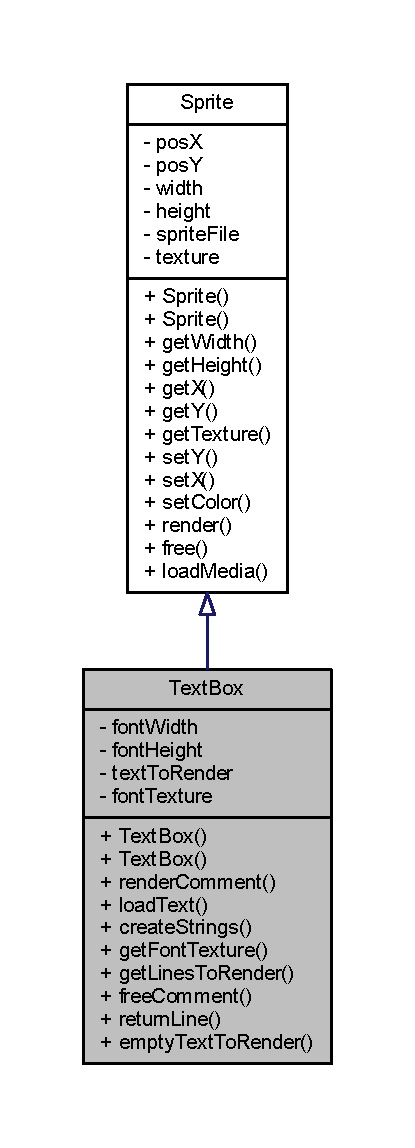
\includegraphics[height=550pt]{class_text_box__inherit__graph}
\end{center}
\end{figure}


Collaboration diagram for Text\+Box\+:\nopagebreak
\begin{figure}[H]
\begin{center}
\leavevmode
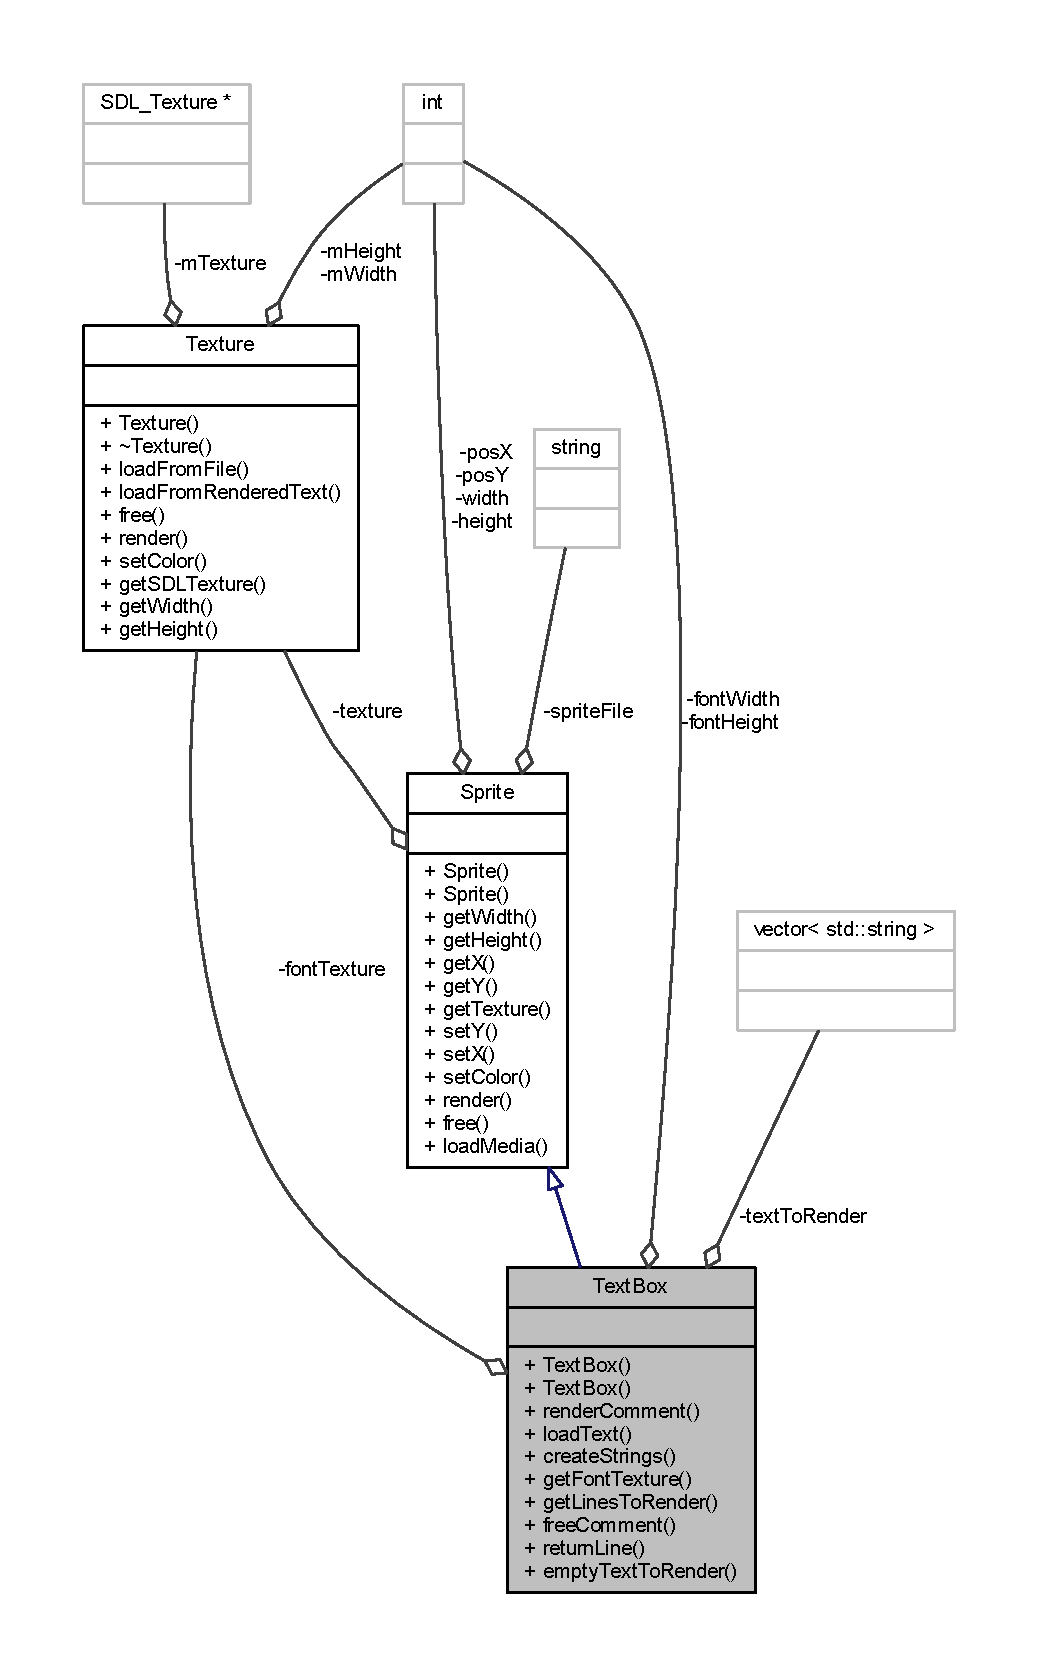
\includegraphics[height=550pt]{class_text_box__coll__graph}
\end{center}
\end{figure}
\subsection*{Public Member Functions}
\begin{DoxyCompactItemize}
\item 
\hyperlink{class_text_box_a25b67e5ff6788c60b8aef3f3540879d0}{Text\+Box} ()
\item 
\hyperlink{class_text_box_a7e80f260cc97085b70e838f0f4250697}{Text\+Box} (std\+::string file\+Name, S\+D\+L\+\_\+\+Renderer $\ast$renderer, int x, int y)
\item 
void \hyperlink{class_text_box_a8746fe595a510ea6c3dc9908b448802c}{render\+Comment} (S\+D\+L\+\_\+\+Renderer $\ast$renderer)
\item 
bool \hyperlink{class_text_box_add2f877e6715744908d5eb0c9c53e5a9}{load\+Text} (S\+D\+L\+\_\+\+Renderer $\ast$renderer, std\+::string text, T\+T\+F\+\_\+\+Font $\ast$font)
\item 
void \hyperlink{class_text_box_a19cb5e85c864060ecdb2fe2bab6fd54d}{create\+Strings} (std\+::string text, T\+T\+F\+\_\+\+Font $\ast$font)
\item 
\hyperlink{class_texture}{Texture} \hyperlink{class_text_box_a47653c059e6074242066423bad187fb6}{get\+Font\+Texture} ()
\item 
int \hyperlink{class_text_box_a7c620113713b6b841ef7e183c1d81312}{get\+Lines\+To\+Render} ()
\item 
void \hyperlink{class_text_box_a6ab09c23671be63b41bd0eba32d385e3}{free\+Comment} ()
\item 
std\+::string \hyperlink{class_text_box_ac10a24236f968ae36705f8bf300dfd79}{return\+Line} (int i)
\item 
void \hyperlink{class_text_box_a3c57ce309c31e346dbc504b5e23d7ebc}{empty\+Text\+To\+Render} ()
\end{DoxyCompactItemize}
\subsection*{Private Attributes}
\begin{DoxyCompactItemize}
\item 
int \hyperlink{class_text_box_a55045d04b5804c912bd9be29bc8478b9}{font\+Width}
\item 
int \hyperlink{class_text_box_a55689185cc0627e45b0d70304eb962d2}{font\+Height}
\item 
std\+::vector$<$ std\+::string $>$ \hyperlink{class_text_box_a13ec32aabf23db2253af70f19a2bf1e9}{text\+To\+Render}
\item 
\hyperlink{class_texture}{Texture} \hyperlink{class_text_box_a94e1863fccbb2e8de3547aa89b8e85f0}{font\+Texture}
\end{DoxyCompactItemize}


\subsection{Detailed Description}
Inherit\textquotesingle{}s from the base sprite class, handles text rendering to the screen, and freeing up that text 

Definition at line 11 of file Text\+Box.\+h.



\subsection{Constructor \& Destructor Documentation}
\mbox{\Hypertarget{class_text_box_a25b67e5ff6788c60b8aef3f3540879d0}\label{class_text_box_a25b67e5ff6788c60b8aef3f3540879d0}} 
\index{Text\+Box@{Text\+Box}!Text\+Box@{Text\+Box}}
\index{Text\+Box@{Text\+Box}!Text\+Box@{Text\+Box}}
\subsubsection{\texorpdfstring{Text\+Box()}{TextBox()}\hspace{0.1cm}{\footnotesize\ttfamily [1/2]}}
{\footnotesize\ttfamily Text\+Box\+::\+Text\+Box (\begin{DoxyParamCaption}{ }\end{DoxyParamCaption})}



Definition at line 3 of file Text\+Box.\+cpp.


\begin{DoxyCode}
3 \{\}
\end{DoxyCode}
\mbox{\Hypertarget{class_text_box_a7e80f260cc97085b70e838f0f4250697}\label{class_text_box_a7e80f260cc97085b70e838f0f4250697}} 
\index{Text\+Box@{Text\+Box}!Text\+Box@{Text\+Box}}
\index{Text\+Box@{Text\+Box}!Text\+Box@{Text\+Box}}
\subsubsection{\texorpdfstring{Text\+Box()}{TextBox()}\hspace{0.1cm}{\footnotesize\ttfamily [2/2]}}
{\footnotesize\ttfamily Text\+Box\+::\+Text\+Box (\begin{DoxyParamCaption}\item[{std\+::string}]{file\+Name,  }\item[{S\+D\+L\+\_\+\+Renderer $\ast$}]{renderer,  }\item[{int}]{x,  }\item[{int}]{y }\end{DoxyParamCaption})}



Definition at line 5 of file Text\+Box.\+cpp.


\begin{DoxyCode}
5 : \hyperlink{class_sprite_a12cba3ac1868418add3c4d95ce87e615}{Sprite}(fileName, renderer, x, y)\{\}
\end{DoxyCode}


\subsection{Member Function Documentation}
\mbox{\Hypertarget{class_text_box_a19cb5e85c864060ecdb2fe2bab6fd54d}\label{class_text_box_a19cb5e85c864060ecdb2fe2bab6fd54d}} 
\index{Text\+Box@{Text\+Box}!create\+Strings@{create\+Strings}}
\index{create\+Strings@{create\+Strings}!Text\+Box@{Text\+Box}}
\subsubsection{\texorpdfstring{create\+Strings()}{createStrings()}}
{\footnotesize\ttfamily void Text\+Box\+::create\+Strings (\begin{DoxyParamCaption}\item[{std\+::string}]{text,  }\item[{T\+T\+F\+\_\+\+Font $\ast$}]{font }\end{DoxyParamCaption})}

Breaks up text into 3 line chunks to be rendered \begin{DoxyRefDesc}{Bug}
\item[\hyperlink{bug__bug000001}{Bug}]There is currently an issue where the texture will return 0, temp fix has been implemented where the texture width is hardcoded \end{DoxyRefDesc}


Definition at line 50 of file Text\+Box.\+cpp.



References Sprite\+::get\+Width(), and text\+To\+Render.



Referenced by N\+P\+C\+::prepare\+Comment().


\begin{DoxyCode}
51 \{
52     \textcolor{keywordflow}{if} (font == NULL)
53     \{
54         printf(\textcolor{stringliteral}{"Failed to load font! SDL\_ttf Error: %s\(\backslash\)n"}, TTF\_GetError());
55     \}
56     \textcolor{keywordflow}{else}
57     \{
58         \textcolor{keywordflow}{try}
59         \{
60             \textcolor{comment}{// Find the dimensions of a single character rendered in the parsed in font}
61             \textcolor{keywordtype}{int} tW, tH;
62             TTF\_SizeText(font, \textcolor{stringliteral}{"a"}, &tW, &tH);
63 
64             \textcolor{comment}{// retrieve the width of our texture}
65             \textcolor{keywordtype}{int} supposedWidth = \hyperlink{class_sprite_aba3d4752461ec679fbf5de7ec4c34f61}{getWidth}();
66             
68             \textcolor{keywordtype}{int} maxCharsPerLine = 180 / tW;
69 
70             \textcolor{keywordflow}{if} (maxCharsPerLine == 0)
71                 \textcolor{keywordflow}{throw} std::overflow\_error(\textcolor{stringliteral}{"texture Width is 0!"});
72             
73             \textcolor{comment}{// Divide the length of text by the max number of chars that can be had per line}
74             \textcolor{keywordtype}{int} numSubStrings = text.length() / maxCharsPerLine;
75             std::vector<std::string> ret;
76 
77 
78             std::stringstream threeChunks;
79             \textcolor{keywordtype}{int} counter = 0;
80             \textcolor{keywordflow}{for} (\textcolor{keywordtype}{int} i = 0; i < numSubStrings; i++)
81             \{
82                 \textcolor{comment}{// Create a substring using the maxCharPerLine value }
83                 std::string textChunk = text.substr(i * maxCharsPerLine, maxCharsPerLine);
84 
85                 \textcolor{comment}{// feed the chunk into our string stream}
86                 threeChunks << textChunk;
87                 counter++;
88 
89                 \textcolor{comment}{// if we have 3 lines stored, push back the chunk}
90                 \textcolor{keywordflow}{if} (counter == 3 || counter == numSubStrings)
91                 \{
92                     counter = 0;
93                     \hyperlink{class_text_box_a13ec32aabf23db2253af70f19a2bf1e9}{textToRender}.push\_back(threeChunks.str());
94                     threeChunks.str(\textcolor{stringliteral}{""});
95                 \}
96             \}
97 
98             \textcolor{comment}{// add the remainder text as a chunk}
99             \textcolor{keywordflow}{if} (text.length() % maxCharsPerLine != 0)
100             \{
101                 threeChunks << text.substr(maxCharsPerLine * numSubStrings);
102                 \hyperlink{class_text_box_a13ec32aabf23db2253af70f19a2bf1e9}{textToRender}.push\_back(threeChunks.str());
103                 threeChunks.str(\textcolor{stringliteral}{""});
104             \}
105         \}
106         \textcolor{keywordflow}{catch} (std::overflow\_error e)
107         \{
108             std::cout << e.what() << std::endl;;
109         \}
110     \}
111 \}
\end{DoxyCode}
\mbox{\Hypertarget{class_text_box_a3c57ce309c31e346dbc504b5e23d7ebc}\label{class_text_box_a3c57ce309c31e346dbc504b5e23d7ebc}} 
\index{Text\+Box@{Text\+Box}!empty\+Text\+To\+Render@{empty\+Text\+To\+Render}}
\index{empty\+Text\+To\+Render@{empty\+Text\+To\+Render}!Text\+Box@{Text\+Box}}
\subsubsection{\texorpdfstring{empty\+Text\+To\+Render()}{emptyTextToRender()}}
{\footnotesize\ttfamily void Text\+Box\+::empty\+Text\+To\+Render (\begin{DoxyParamCaption}{ }\end{DoxyParamCaption})}



Definition at line 131 of file Text\+Box.\+cpp.



References text\+To\+Render.



Referenced by N\+P\+C\+::prepare\+Comment().


\begin{DoxyCode}
132 \{
133     \hyperlink{class_text_box_a13ec32aabf23db2253af70f19a2bf1e9}{textToRender}.clear();
134 \}
\end{DoxyCode}
\mbox{\Hypertarget{class_text_box_a6ab09c23671be63b41bd0eba32d385e3}\label{class_text_box_a6ab09c23671be63b41bd0eba32d385e3}} 
\index{Text\+Box@{Text\+Box}!free\+Comment@{free\+Comment}}
\index{free\+Comment@{free\+Comment}!Text\+Box@{Text\+Box}}
\subsubsection{\texorpdfstring{free\+Comment()}{freeComment()}}
{\footnotesize\ttfamily void Text\+Box\+::free\+Comment (\begin{DoxyParamCaption}{ }\end{DoxyParamCaption})}



Definition at line 113 of file Text\+Box.\+cpp.



References font\+Texture, and Texture\+::free().



Referenced by N\+P\+C\+::free\+Box().


\begin{DoxyCode}
114 \{
115     \hyperlink{class_text_box_a94e1863fccbb2e8de3547aa89b8e85f0}{fontTexture}.\hyperlink{class_texture_a46d06aec832e5a954f1c8ca957c2c6e5}{free}();
116 \}
\end{DoxyCode}
\mbox{\Hypertarget{class_text_box_a47653c059e6074242066423bad187fb6}\label{class_text_box_a47653c059e6074242066423bad187fb6}} 
\index{Text\+Box@{Text\+Box}!get\+Font\+Texture@{get\+Font\+Texture}}
\index{get\+Font\+Texture@{get\+Font\+Texture}!Text\+Box@{Text\+Box}}
\subsubsection{\texorpdfstring{get\+Font\+Texture()}{getFontTexture()}}
{\footnotesize\ttfamily \hyperlink{class_texture}{Texture} Text\+Box\+::get\+Font\+Texture (\begin{DoxyParamCaption}{ }\end{DoxyParamCaption})}



Definition at line 12 of file Text\+Box.\+cpp.



References font\+Texture.


\begin{DoxyCode}
13 \{
14     \textcolor{keywordflow}{return} \hyperlink{class_text_box_a94e1863fccbb2e8de3547aa89b8e85f0}{fontTexture};
15 \}
\end{DoxyCode}
\mbox{\Hypertarget{class_text_box_a7c620113713b6b841ef7e183c1d81312}\label{class_text_box_a7c620113713b6b841ef7e183c1d81312}} 
\index{Text\+Box@{Text\+Box}!get\+Lines\+To\+Render@{get\+Lines\+To\+Render}}
\index{get\+Lines\+To\+Render@{get\+Lines\+To\+Render}!Text\+Box@{Text\+Box}}
\subsubsection{\texorpdfstring{get\+Lines\+To\+Render()}{getLinesToRender()}}
{\footnotesize\ttfamily int Text\+Box\+::get\+Lines\+To\+Render (\begin{DoxyParamCaption}{ }\end{DoxyParamCaption})}



Definition at line 118 of file Text\+Box.\+cpp.



References text\+To\+Render.



Referenced by N\+P\+C\+::get\+Lines\+To\+Render().


\begin{DoxyCode}
119 \{
120     \textcolor{keywordflow}{return} \hyperlink{class_text_box_a13ec32aabf23db2253af70f19a2bf1e9}{textToRender}.size();
121 \}
\end{DoxyCode}
\mbox{\Hypertarget{class_text_box_add2f877e6715744908d5eb0c9c53e5a9}\label{class_text_box_add2f877e6715744908d5eb0c9c53e5a9}} 
\index{Text\+Box@{Text\+Box}!load\+Text@{load\+Text}}
\index{load\+Text@{load\+Text}!Text\+Box@{Text\+Box}}
\subsubsection{\texorpdfstring{load\+Text()}{loadText()}}
{\footnotesize\ttfamily bool Text\+Box\+::load\+Text (\begin{DoxyParamCaption}\item[{S\+D\+L\+\_\+\+Renderer $\ast$}]{renderer,  }\item[{std\+::string}]{text,  }\item[{T\+T\+F\+\_\+\+Font $\ast$}]{font }\end{DoxyParamCaption})}

Load parsed in text as a texture 

Definition at line 20 of file Text\+Box.\+cpp.



References font\+Height, font\+Texture, font\+Width, Texture\+::get\+Height(), Sprite\+::get\+Width(), Texture\+::get\+Width(), and Texture\+::load\+From\+Rendered\+Text().



Referenced by N\+P\+C\+::\+Load\+Comment().


\begin{DoxyCode}
21 \{
22     \textcolor{comment}{//Loading success flag}
23     \textcolor{keywordtype}{bool} success = \textcolor{keyword}{true};
24 
25     \textcolor{comment}{//Open the font}
26     \textcolor{keywordflow}{if} (font == NULL)
27     \{
28         printf(\textcolor{stringliteral}{"Failed to load font! SDL\_ttf Error: %s\(\backslash\)n"}, TTF\_GetError());
29         success = \textcolor{keyword}{false};
30     \}
31     \textcolor{keywordflow}{else}
32     \{
33         \textcolor{comment}{//Render text}
34         SDL\_Color textColor = \{ 0, 0, 0 \};
35         \textcolor{keywordflow}{if} (!\hyperlink{class_text_box_a94e1863fccbb2e8de3547aa89b8e85f0}{fontTexture}.\hyperlink{class_texture_a78708fd59f16721c2c19b2075a91e1bc}{loadFromRenderedText}(text, textColor, renderer, 
      font, \hyperlink{class_sprite_aba3d4752461ec679fbf5de7ec4c34f61}{getWidth}()))
36         \{
37             printf(\textcolor{stringliteral}{"Failed to render text texture!\(\backslash\)n"});
38             success = \textcolor{keyword}{false};
39         \}
40         \hyperlink{class_text_box_a55045d04b5804c912bd9be29bc8478b9}{fontWidth} = \hyperlink{class_text_box_a94e1863fccbb2e8de3547aa89b8e85f0}{fontTexture}.\hyperlink{class_texture_a91a6fd3355bc870194851514194daaab}{getWidth}();
41         \hyperlink{class_text_box_a55689185cc0627e45b0d70304eb962d2}{fontHeight} = \hyperlink{class_text_box_a94e1863fccbb2e8de3547aa89b8e85f0}{fontTexture}.\hyperlink{class_texture_a80e143905655b173df5994300088ce35}{getHeight}();
42     \}
43 
44     \textcolor{keywordflow}{return} success;
45 \}
\end{DoxyCode}
\mbox{\Hypertarget{class_text_box_a8746fe595a510ea6c3dc9908b448802c}\label{class_text_box_a8746fe595a510ea6c3dc9908b448802c}} 
\index{Text\+Box@{Text\+Box}!render\+Comment@{render\+Comment}}
\index{render\+Comment@{render\+Comment}!Text\+Box@{Text\+Box}}
\subsubsection{\texorpdfstring{render\+Comment()}{renderComment()}}
{\footnotesize\ttfamily void Text\+Box\+::render\+Comment (\begin{DoxyParamCaption}\item[{S\+D\+L\+\_\+\+Renderer $\ast$}]{renderer }\end{DoxyParamCaption})}



Definition at line 7 of file Text\+Box.\+cpp.



References font\+Texture, Sprite\+::get\+X(), Sprite\+::get\+Y(), and Texture\+::render().



Referenced by N\+P\+C\+::render\+Comment().


\begin{DoxyCode}
8 \{
9     \hyperlink{class_text_box_a94e1863fccbb2e8de3547aa89b8e85f0}{fontTexture}.\hyperlink{class_texture_ac91a5257c451c80ffbf9a3d1485ba1c8}{render}(\hyperlink{class_sprite_a03d6c82bddfd3d164ce8997482c57c85}{getX}(), \hyperlink{class_sprite_a53ea8b27bcd0dab0627a2dceab2b9d98}{getY}(), renderer);
10 \}
\end{DoxyCode}
\mbox{\Hypertarget{class_text_box_ac10a24236f968ae36705f8bf300dfd79}\label{class_text_box_ac10a24236f968ae36705f8bf300dfd79}} 
\index{Text\+Box@{Text\+Box}!return\+Line@{return\+Line}}
\index{return\+Line@{return\+Line}!Text\+Box@{Text\+Box}}
\subsubsection{\texorpdfstring{return\+Line()}{returnLine()}}
{\footnotesize\ttfamily std\+::string Text\+Box\+::return\+Line (\begin{DoxyParamCaption}\item[{int}]{i }\end{DoxyParamCaption})}



Definition at line 123 of file Text\+Box.\+cpp.



References text\+To\+Render.



Referenced by N\+P\+C\+::\+Load\+Comment().


\begin{DoxyCode}
124 \{
125     \textcolor{keywordflow}{if} (\hyperlink{class_text_box_a13ec32aabf23db2253af70f19a2bf1e9}{textToRender}.size() > 0)
126         \textcolor{keywordflow}{return} \hyperlink{class_text_box_a13ec32aabf23db2253af70f19a2bf1e9}{textToRender}[i];
127     \textcolor{keywordflow}{else}
128         \textcolor{keywordflow}{return} \textcolor{stringliteral}{""};
129 \}
\end{DoxyCode}


\subsection{Member Data Documentation}
\mbox{\Hypertarget{class_text_box_a55689185cc0627e45b0d70304eb962d2}\label{class_text_box_a55689185cc0627e45b0d70304eb962d2}} 
\index{Text\+Box@{Text\+Box}!font\+Height@{font\+Height}}
\index{font\+Height@{font\+Height}!Text\+Box@{Text\+Box}}
\subsubsection{\texorpdfstring{font\+Height}{fontHeight}}
{\footnotesize\ttfamily int Text\+Box\+::font\+Height\hspace{0.3cm}{\ttfamily [private]}}



Definition at line 30 of file Text\+Box.\+h.



Referenced by load\+Text().

\mbox{\Hypertarget{class_text_box_a94e1863fccbb2e8de3547aa89b8e85f0}\label{class_text_box_a94e1863fccbb2e8de3547aa89b8e85f0}} 
\index{Text\+Box@{Text\+Box}!font\+Texture@{font\+Texture}}
\index{font\+Texture@{font\+Texture}!Text\+Box@{Text\+Box}}
\subsubsection{\texorpdfstring{font\+Texture}{fontTexture}}
{\footnotesize\ttfamily \hyperlink{class_texture}{Texture} Text\+Box\+::font\+Texture\hspace{0.3cm}{\ttfamily [private]}}



Definition at line 33 of file Text\+Box.\+h.



Referenced by free\+Comment(), get\+Font\+Texture(), load\+Text(), and render\+Comment().

\mbox{\Hypertarget{class_text_box_a55045d04b5804c912bd9be29bc8478b9}\label{class_text_box_a55045d04b5804c912bd9be29bc8478b9}} 
\index{Text\+Box@{Text\+Box}!font\+Width@{font\+Width}}
\index{font\+Width@{font\+Width}!Text\+Box@{Text\+Box}}
\subsubsection{\texorpdfstring{font\+Width}{fontWidth}}
{\footnotesize\ttfamily int Text\+Box\+::font\+Width\hspace{0.3cm}{\ttfamily [private]}}



Definition at line 30 of file Text\+Box.\+h.



Referenced by load\+Text().

\mbox{\Hypertarget{class_text_box_a13ec32aabf23db2253af70f19a2bf1e9}\label{class_text_box_a13ec32aabf23db2253af70f19a2bf1e9}} 
\index{Text\+Box@{Text\+Box}!text\+To\+Render@{text\+To\+Render}}
\index{text\+To\+Render@{text\+To\+Render}!Text\+Box@{Text\+Box}}
\subsubsection{\texorpdfstring{text\+To\+Render}{textToRender}}
{\footnotesize\ttfamily std\+::vector$<$std\+::string$>$ Text\+Box\+::text\+To\+Render\hspace{0.3cm}{\ttfamily [private]}}



Definition at line 32 of file Text\+Box.\+h.



Referenced by create\+Strings(), empty\+Text\+To\+Render(), get\+Lines\+To\+Render(), and return\+Line().



The documentation for this class was generated from the following files\+:\begin{DoxyCompactItemize}
\item 
C\+:/\+Users/\+Kyle Tuckey/\+Documents/\+Final Year Project/\+Social\+\_\+\+N\+P\+C\+S/\+Social\+\_\+\+N\+P\+C\+S/\hyperlink{_text_box_8h}{Text\+Box.\+h}\item 
C\+:/\+Users/\+Kyle Tuckey/\+Documents/\+Final Year Project/\+Social\+\_\+\+N\+P\+C\+S/\+Social\+\_\+\+N\+P\+C\+S/\hyperlink{_text_box_8cpp}{Text\+Box.\+cpp}\end{DoxyCompactItemize}

\hypertarget{class_texture}{}\section{Texture Class Reference}
\label{class_texture}\index{Texture@{Texture}}


{\ttfamily \#include $<$Texture.\+h$>$}



Collaboration diagram for Texture\+:\nopagebreak
\begin{figure}[H]
\begin{center}
\leavevmode
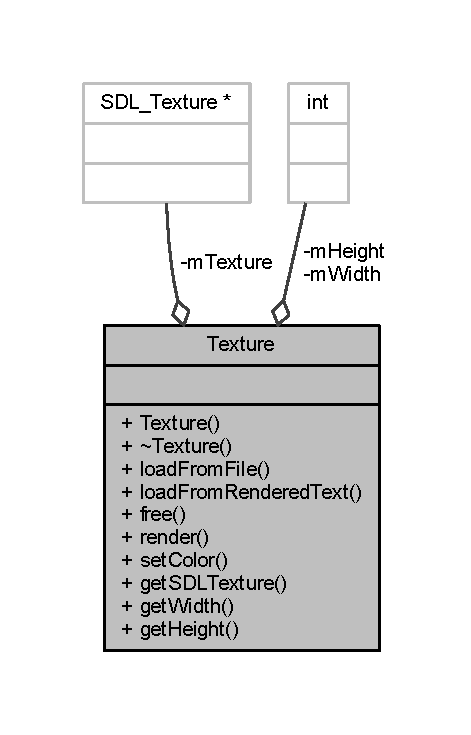
\includegraphics[width=226pt]{class_texture__coll__graph}
\end{center}
\end{figure}
\subsection*{Public Member Functions}
\begin{DoxyCompactItemize}
\item 
\hyperlink{class_texture_a6c275e3f186675ff6ed73ccf970e552f}{Texture} ()
\item 
\hyperlink{class_texture_a09c4bcb7462f64c1d20fa69dba3cee8a}{$\sim$\+Texture} ()
\item 
bool \hyperlink{class_texture_a1c143b8aa5f134bb5a8c9d4c3d950d2f}{load\+From\+File} (std\+::string path, S\+D\+L\+\_\+\+Renderer $\ast$renderer)
\begin{DoxyCompactList}\small\item\em Loads image at specified path. \end{DoxyCompactList}\item 
bool \hyperlink{class_texture_a78708fd59f16721c2c19b2075a91e1bc}{load\+From\+Rendered\+Text} (std\+::string texture\+Text, S\+D\+L\+\_\+\+Color text\+Color, S\+D\+L\+\_\+\+Renderer $\ast$renderer, T\+T\+F\+\_\+\+Font $\ast$g\+Font, int wrap\+Length)
\begin{DoxyCompactList}\small\item\em Creates image from font string. \end{DoxyCompactList}\item 
void \hyperlink{class_texture_a46d06aec832e5a954f1c8ca957c2c6e5}{free} ()
\begin{DoxyCompactList}\small\item\em Deallocates texture. \end{DoxyCompactList}\item 
void \hyperlink{class_texture_ac91a5257c451c80ffbf9a3d1485ba1c8}{render} (int x, int y, S\+D\+L\+\_\+\+Renderer $\ast$renderer, S\+D\+L\+\_\+\+Rect $\ast$clip=N\+U\+LL, double angle=0.\+0, S\+D\+L\+\_\+\+Point $\ast$center=N\+U\+LL, S\+D\+L\+\_\+\+Renderer\+Flip flip=S\+D\+L\+\_\+\+F\+L\+I\+P\+\_\+\+N\+O\+NE)
\begin{DoxyCompactList}\small\item\em Renders texture at given point. \end{DoxyCompactList}\item 
void \hyperlink{class_texture_ab3149eb648f437a09dc0938942c2c4ce}{set\+Color} (int r, int g, int b)
\begin{DoxyCompactList}\small\item\em sets the sprites R\+BG values \end{DoxyCompactList}\item 
S\+D\+L\+\_\+\+Texture $\ast$ \hyperlink{class_texture_a4c7638bab72e620b54cd8224019eb3dd}{get\+S\+D\+L\+Texture} ()
\begin{DoxyCompactList}\small\item\em returns the S\+DL texture \end{DoxyCompactList}\item 
int \hyperlink{class_texture_a91a6fd3355bc870194851514194daaab}{get\+Width} ()
\begin{DoxyCompactList}\small\item\em Gets image width. \end{DoxyCompactList}\item 
int \hyperlink{class_texture_a80e143905655b173df5994300088ce35}{get\+Height} ()
\begin{DoxyCompactList}\small\item\em Gets image height. \end{DoxyCompactList}\end{DoxyCompactItemize}
\subsection*{Private Attributes}
\begin{DoxyCompactItemize}
\item 
S\+D\+L\+\_\+\+Texture $\ast$ \hyperlink{class_texture_a28e61626f21dd1c69968e53687a13424}{m\+Texture}
\begin{DoxyCompactList}\small\item\em The actual hardware texture. \end{DoxyCompactList}\item 
int \hyperlink{class_texture_a0e007f4b4f1a314e5b0dae1402a13afb}{m\+Width}
\begin{DoxyCompactList}\small\item\em Image dimensions. \end{DoxyCompactList}\item 
int \hyperlink{class_texture_ad7078e03c0ef6e69b733eb85fd72aec2}{m\+Height}
\end{DoxyCompactItemize}


\subsection{Detailed Description}
Implementation is based on the L\+Texture class from \href{http://lazyfoo.net/tutorials/SDL/12_color_modulation/index.php}{\tt http\+://lazyfoo.\+net/tutorials/\+S\+D\+L/12\+\_\+color\+\_\+modulation/index.\+php} it is a wrapper surrounding the S\+D\+L\+\_\+\+Texture class 

Definition at line 13 of file Texture.\+h.



\subsection{Constructor \& Destructor Documentation}
\mbox{\Hypertarget{class_texture_a6c275e3f186675ff6ed73ccf970e552f}\label{class_texture_a6c275e3f186675ff6ed73ccf970e552f}} 
\index{Texture@{Texture}!Texture@{Texture}}
\index{Texture@{Texture}!Texture@{Texture}}
\subsubsection{\texorpdfstring{Texture()}{Texture()}}
{\footnotesize\ttfamily Texture\+::\+Texture (\begin{DoxyParamCaption}{ }\end{DoxyParamCaption})}



Definition at line 5 of file Texture.\+cpp.



References m\+Height, m\+Texture, and m\+Width.


\begin{DoxyCode}
6 \{
7     \textcolor{comment}{//Initialize}
8     \hyperlink{class_texture_a28e61626f21dd1c69968e53687a13424}{mTexture} = NULL;
9     \hyperlink{class_texture_a0e007f4b4f1a314e5b0dae1402a13afb}{mWidth} = 0;
10     \hyperlink{class_texture_ad7078e03c0ef6e69b733eb85fd72aec2}{mHeight} = 0;
11 \}
\end{DoxyCode}
\mbox{\Hypertarget{class_texture_a09c4bcb7462f64c1d20fa69dba3cee8a}\label{class_texture_a09c4bcb7462f64c1d20fa69dba3cee8a}} 
\index{Texture@{Texture}!````~Texture@{$\sim$\+Texture}}
\index{````~Texture@{$\sim$\+Texture}!Texture@{Texture}}
\subsubsection{\texorpdfstring{$\sim$\+Texture()}{~Texture()}}
{\footnotesize\ttfamily Texture\+::$\sim$\+Texture (\begin{DoxyParamCaption}{ }\end{DoxyParamCaption})}



Definition at line 14 of file Texture.\+cpp.



References free().


\begin{DoxyCode}
15 \{
16     \textcolor{comment}{//Deallocate}
17     \hyperlink{class_texture_a46d06aec832e5a954f1c8ca957c2c6e5}{free}();
18 \}
\end{DoxyCode}


\subsection{Member Function Documentation}
\mbox{\Hypertarget{class_texture_a46d06aec832e5a954f1c8ca957c2c6e5}\label{class_texture_a46d06aec832e5a954f1c8ca957c2c6e5}} 
\index{Texture@{Texture}!free@{free}}
\index{free@{free}!Texture@{Texture}}
\subsubsection{\texorpdfstring{free()}{free()}}
{\footnotesize\ttfamily void Texture\+::free (\begin{DoxyParamCaption}{ }\end{DoxyParamCaption})}



Deallocates texture. 

Frees up the memory space the texture is occupying 

Definition at line 114 of file Texture.\+cpp.



References m\+Texture.



Referenced by Sprite\+::free(), Text\+Box\+::free\+Comment(), load\+From\+File(), load\+From\+Rendered\+Text(), and $\sim$\+Texture().


\begin{DoxyCode}
115 \{
116     \textcolor{comment}{//Free texture if it exists}
117     \textcolor{keywordflow}{if} (\hyperlink{class_texture_a28e61626f21dd1c69968e53687a13424}{mTexture} != NULL)
118     \{
119         SDL\_DestroyTexture(\hyperlink{class_texture_a28e61626f21dd1c69968e53687a13424}{mTexture});
120         \hyperlink{class_texture_a28e61626f21dd1c69968e53687a13424}{mTexture} = NULL;
121     \}
122 \}
\end{DoxyCode}
\mbox{\Hypertarget{class_texture_a80e143905655b173df5994300088ce35}\label{class_texture_a80e143905655b173df5994300088ce35}} 
\index{Texture@{Texture}!get\+Height@{get\+Height}}
\index{get\+Height@{get\+Height}!Texture@{Texture}}
\subsubsection{\texorpdfstring{get\+Height()}{getHeight()}}
{\footnotesize\ttfamily int Texture\+::get\+Height (\begin{DoxyParamCaption}{ }\end{DoxyParamCaption})}



Gets image height. 

get the Textures height 

Definition at line 164 of file Texture.\+cpp.



References m\+Texture.



Referenced by Sprite\+::load\+Media(), and Text\+Box\+::load\+Text().


\begin{DoxyCode}
165 \{
166     \textcolor{keywordtype}{int} w, h;
167     SDL\_QueryTexture(\hyperlink{class_texture_a28e61626f21dd1c69968e53687a13424}{mTexture}, NULL, NULL, &w, &h);
168     \textcolor{keywordflow}{return} h;
169 \}
\end{DoxyCode}
\mbox{\Hypertarget{class_texture_a4c7638bab72e620b54cd8224019eb3dd}\label{class_texture_a4c7638bab72e620b54cd8224019eb3dd}} 
\index{Texture@{Texture}!get\+S\+D\+L\+Texture@{get\+S\+D\+L\+Texture}}
\index{get\+S\+D\+L\+Texture@{get\+S\+D\+L\+Texture}!Texture@{Texture}}
\subsubsection{\texorpdfstring{get\+S\+D\+L\+Texture()}{getSDLTexture()}}
{\footnotesize\ttfamily S\+D\+L\+\_\+\+Texture $\ast$ Texture\+::get\+S\+D\+L\+Texture (\begin{DoxyParamCaption}{ }\end{DoxyParamCaption})}



returns the S\+DL texture 

Return the S\+D\+L\+\_\+\+Texture pointer 

Definition at line 67 of file Texture.\+cpp.



References m\+Texture.


\begin{DoxyCode}
68 \{
69     \textcolor{keywordflow}{return} \hyperlink{class_texture_a28e61626f21dd1c69968e53687a13424}{mTexture};
70 \}
\end{DoxyCode}
\mbox{\Hypertarget{class_texture_a91a6fd3355bc870194851514194daaab}\label{class_texture_a91a6fd3355bc870194851514194daaab}} 
\index{Texture@{Texture}!get\+Width@{get\+Width}}
\index{get\+Width@{get\+Width}!Texture@{Texture}}
\subsubsection{\texorpdfstring{get\+Width()}{getWidth()}}
{\footnotesize\ttfamily int Texture\+::get\+Width (\begin{DoxyParamCaption}{ }\end{DoxyParamCaption})}



Gets image width. 

get the Textures width 

Definition at line 154 of file Texture.\+cpp.



References m\+Texture.



Referenced by Sprite\+::load\+Media(), and Text\+Box\+::load\+Text().


\begin{DoxyCode}
155 \{
156     \textcolor{keywordtype}{int} w, h;
157     SDL\_QueryTexture(\hyperlink{class_texture_a28e61626f21dd1c69968e53687a13424}{mTexture}, NULL, NULL, &w, &h);
158     \textcolor{keywordflow}{return} w;
159 \}
\end{DoxyCode}
\mbox{\Hypertarget{class_texture_a1c143b8aa5f134bb5a8c9d4c3d950d2f}\label{class_texture_a1c143b8aa5f134bb5a8c9d4c3d950d2f}} 
\index{Texture@{Texture}!load\+From\+File@{load\+From\+File}}
\index{load\+From\+File@{load\+From\+File}!Texture@{Texture}}
\subsubsection{\texorpdfstring{load\+From\+File()}{loadFromFile()}}
{\footnotesize\ttfamily bool Texture\+::load\+From\+File (\begin{DoxyParamCaption}\item[{std\+::string}]{path,  }\item[{S\+D\+L\+\_\+\+Renderer $\ast$}]{renderer }\end{DoxyParamCaption})}



Loads image at specified path. 

Loads in a P\+NG images as a texture to the game 

Definition at line 23 of file Texture.\+cpp.



References free(), m\+Height, m\+Texture, and m\+Width.



Referenced by Sprite\+::load\+Media().


\begin{DoxyCode}
24 \{
25     \textcolor{comment}{//Get rid of preexisting texture}
26     \hyperlink{class_texture_a46d06aec832e5a954f1c8ca957c2c6e5}{free}();
27 
28     \textcolor{comment}{//The final texture}
29     SDL\_Texture* newTexture = NULL;
30 
31     \textcolor{comment}{//Load image at specified path}
32     SDL\_Surface* loadedSurface = IMG\_Load(path.c\_str());
33     \textcolor{keywordflow}{if} (loadedSurface == NULL)
34     \{
35         printf(\textcolor{stringliteral}{"Unable to load image %s! SDL\_image Error: %s\(\backslash\)n"}, path.c\_str(), IMG\_GetError());
36     \}
37     \textcolor{keywordflow}{else}
38     \{
39         \textcolor{comment}{//Color key image}
40         SDL\_SetColorKey(loadedSurface, SDL\_TRUE, SDL\_MapRGB(loadedSurface->format, 0, 0xFF, 0xFF));
41 
42         \textcolor{comment}{//Create texture from surface pixels}
43         newTexture = SDL\_CreateTextureFromSurface(renderer, loadedSurface);
44         \textcolor{keywordflow}{if} (newTexture == NULL)
45         \{
46             printf(\textcolor{stringliteral}{"Unable to create texture from %s! SDL Error: %s\(\backslash\)n"}, path.c\_str(), SDL\_GetError());
47         \}
48         \textcolor{keywordflow}{else}
49         \{
50             \textcolor{comment}{//Get image dimensions}
51             \hyperlink{class_texture_a0e007f4b4f1a314e5b0dae1402a13afb}{mWidth} = loadedSurface->w;
52             \hyperlink{class_texture_ad7078e03c0ef6e69b733eb85fd72aec2}{mHeight} = loadedSurface->h;
53         \}
54 
55         \textcolor{comment}{//Get rid of old loaded surface}
56         SDL\_FreeSurface(loadedSurface);
57     \}
58 
59     \textcolor{comment}{//Return success}
60     \hyperlink{class_texture_a28e61626f21dd1c69968e53687a13424}{mTexture} = newTexture;
61     \textcolor{keywordflow}{return} \hyperlink{class_texture_a28e61626f21dd1c69968e53687a13424}{mTexture} != NULL;
62 \}
\end{DoxyCode}
\mbox{\Hypertarget{class_texture_a78708fd59f16721c2c19b2075a91e1bc}\label{class_texture_a78708fd59f16721c2c19b2075a91e1bc}} 
\index{Texture@{Texture}!load\+From\+Rendered\+Text@{load\+From\+Rendered\+Text}}
\index{load\+From\+Rendered\+Text@{load\+From\+Rendered\+Text}!Texture@{Texture}}
\subsubsection{\texorpdfstring{load\+From\+Rendered\+Text()}{loadFromRenderedText()}}
{\footnotesize\ttfamily bool Texture\+::load\+From\+Rendered\+Text (\begin{DoxyParamCaption}\item[{std\+::string}]{texture\+Text,  }\item[{S\+D\+L\+\_\+\+Color}]{text\+Color,  }\item[{S\+D\+L\+\_\+\+Renderer $\ast$}]{renderer,  }\item[{T\+T\+F\+\_\+\+Font $\ast$}]{g\+Font,  }\item[{int}]{wrap\+Length }\end{DoxyParamCaption})}



Creates image from font string. 

loads in any parsed in text as a texture, we want the text to wrap depending on width 

Definition at line 75 of file Texture.\+cpp.



References free(), m\+Height, m\+Texture, and m\+Width.



Referenced by Text\+Box\+::load\+Text().


\begin{DoxyCode}
76 \{
77     \textcolor{comment}{//Get rid of preexisting texture}
78     \hyperlink{class_texture_a46d06aec832e5a954f1c8ca957c2c6e5}{free}();
79 
80     \textcolor{comment}{//Render text surface}
81     SDL\_Surface* textSurface = TTF\_RenderText\_Blended\_Wrapped(gFont, textureText.c\_str(), textColor, 
      wrapLength);
82 
83     \textcolor{keywordflow}{if} (textSurface == NULL)
84     \{
85         printf(\textcolor{stringliteral}{"Unable to render text surface! SDL\_ttf Error: %s\(\backslash\)n"}, TTF\_GetError());
86     \}
87     \textcolor{keywordflow}{else}
88     \{
89         
90         \textcolor{comment}{//Create texture from surface pixels}
91         \hyperlink{class_texture_a28e61626f21dd1c69968e53687a13424}{mTexture} = SDL\_CreateTextureFromSurface(renderer, textSurface);
92         \textcolor{keywordflow}{if} (\hyperlink{class_texture_a28e61626f21dd1c69968e53687a13424}{mTexture} == NULL)
93         \{
94             printf(\textcolor{stringliteral}{"Unable to create texture from rendered text! SDL Error: %s\(\backslash\)n"}, SDL\_GetError());
95         \}
96         \textcolor{keywordflow}{else}
97         \{
98             \textcolor{comment}{//Get image dimensions}
99             \hyperlink{class_texture_a0e007f4b4f1a314e5b0dae1402a13afb}{mWidth} = textSurface->w;
100             \hyperlink{class_texture_ad7078e03c0ef6e69b733eb85fd72aec2}{mHeight} = textSurface->h;
101         \}
102 
103         \textcolor{comment}{//Get rid of old surface}
104         SDL\_FreeSurface(textSurface);
105     \}
106 
107     \textcolor{comment}{//Return success}
108     \textcolor{keywordflow}{return} \hyperlink{class_texture_a28e61626f21dd1c69968e53687a13424}{mTexture} != NULL;
109 \}
\end{DoxyCode}
\mbox{\Hypertarget{class_texture_ac91a5257c451c80ffbf9a3d1485ba1c8}\label{class_texture_ac91a5257c451c80ffbf9a3d1485ba1c8}} 
\index{Texture@{Texture}!render@{render}}
\index{render@{render}!Texture@{Texture}}
\subsubsection{\texorpdfstring{render()}{render()}}
{\footnotesize\ttfamily void Texture\+::render (\begin{DoxyParamCaption}\item[{int}]{x,  }\item[{int}]{y,  }\item[{S\+D\+L\+\_\+\+Renderer $\ast$}]{renderer,  }\item[{S\+D\+L\+\_\+\+Rect $\ast$}]{clip = {\ttfamily NULL},  }\item[{double}]{angle = {\ttfamily 0.0},  }\item[{S\+D\+L\+\_\+\+Point $\ast$}]{center = {\ttfamily NULL},  }\item[{S\+D\+L\+\_\+\+Renderer\+Flip}]{flip = {\ttfamily SDL\+\_\+FLIP\+\_\+NONE} }\end{DoxyParamCaption})}



Renders texture at given point. 

Renders the image to the screen 

Definition at line 135 of file Texture.\+cpp.



References m\+Height, m\+Texture, and m\+Width.



Referenced by Sprite\+::render(), and Text\+Box\+::render\+Comment().


\begin{DoxyCode}
136 \{
137     \textcolor{comment}{//Set rendering space and render to screen}
138     SDL\_Rect renderQuad = \{ x, y, \hyperlink{class_texture_a0e007f4b4f1a314e5b0dae1402a13afb}{mWidth}, \hyperlink{class_texture_ad7078e03c0ef6e69b733eb85fd72aec2}{mHeight} \};
139 
140     \textcolor{comment}{//Set clip rendering dimensions}
141     \textcolor{keywordflow}{if} (clip != NULL)
142     \{
143         renderQuad.w = clip->w;
144         renderQuad.h = clip->h;
145     \}
146 
147     \textcolor{comment}{//Render to screen}
148     SDL\_RenderCopyEx(renderer, \hyperlink{class_texture_a28e61626f21dd1c69968e53687a13424}{mTexture}, clip, &renderQuad, angle, center, flip);
149 \}
\end{DoxyCode}
\mbox{\Hypertarget{class_texture_ab3149eb648f437a09dc0938942c2c4ce}\label{class_texture_ab3149eb648f437a09dc0938942c2c4ce}} 
\index{Texture@{Texture}!set\+Color@{set\+Color}}
\index{set\+Color@{set\+Color}!Texture@{Texture}}
\subsubsection{\texorpdfstring{set\+Color()}{setColor()}}
{\footnotesize\ttfamily void Texture\+::set\+Color (\begin{DoxyParamCaption}\item[{int}]{r,  }\item[{int}]{g,  }\item[{int}]{b }\end{DoxyParamCaption})}



sets the sprites R\+BG values 

Modulates the colour of our \hyperlink{class_texture}{Texture} 

Definition at line 127 of file Texture.\+cpp.



References m\+Texture.



Referenced by Sprite\+::set\+Color().


\begin{DoxyCode}
128 \{
129     SDL\_SetTextureColorMod(\hyperlink{class_texture_a28e61626f21dd1c69968e53687a13424}{mTexture}, r, g, b);
130 \}
\end{DoxyCode}


\subsection{Member Data Documentation}
\mbox{\Hypertarget{class_texture_ad7078e03c0ef6e69b733eb85fd72aec2}\label{class_texture_ad7078e03c0ef6e69b733eb85fd72aec2}} 
\index{Texture@{Texture}!m\+Height@{m\+Height}}
\index{m\+Height@{m\+Height}!Texture@{Texture}}
\subsubsection{\texorpdfstring{m\+Height}{mHeight}}
{\footnotesize\ttfamily int Texture\+::m\+Height\hspace{0.3cm}{\ttfamily [private]}}



Definition at line 48 of file Texture.\+h.



Referenced by load\+From\+File(), load\+From\+Rendered\+Text(), render(), and Texture().

\mbox{\Hypertarget{class_texture_a28e61626f21dd1c69968e53687a13424}\label{class_texture_a28e61626f21dd1c69968e53687a13424}} 
\index{Texture@{Texture}!m\+Texture@{m\+Texture}}
\index{m\+Texture@{m\+Texture}!Texture@{Texture}}
\subsubsection{\texorpdfstring{m\+Texture}{mTexture}}
{\footnotesize\ttfamily S\+D\+L\+\_\+\+Texture$\ast$ Texture\+::m\+Texture\hspace{0.3cm}{\ttfamily [private]}}



The actual hardware texture. 



Definition at line 44 of file Texture.\+h.



Referenced by free(), get\+Height(), get\+S\+D\+L\+Texture(), get\+Width(), load\+From\+File(), load\+From\+Rendered\+Text(), render(), set\+Color(), and Texture().

\mbox{\Hypertarget{class_texture_a0e007f4b4f1a314e5b0dae1402a13afb}\label{class_texture_a0e007f4b4f1a314e5b0dae1402a13afb}} 
\index{Texture@{Texture}!m\+Width@{m\+Width}}
\index{m\+Width@{m\+Width}!Texture@{Texture}}
\subsubsection{\texorpdfstring{m\+Width}{mWidth}}
{\footnotesize\ttfamily int Texture\+::m\+Width\hspace{0.3cm}{\ttfamily [private]}}



Image dimensions. 



Definition at line 47 of file Texture.\+h.



Referenced by load\+From\+File(), load\+From\+Rendered\+Text(), render(), and Texture().



The documentation for this class was generated from the following files\+:\begin{DoxyCompactItemize}
\item 
C\+:/\+Users/\+Kyle Tuckey/\+Documents/\+Final Year Project/\+Social\+\_\+\+N\+P\+C\+S/\+Social\+\_\+\+N\+P\+C\+S/\hyperlink{_texture_8h}{Texture.\+h}\item 
C\+:/\+Users/\+Kyle Tuckey/\+Documents/\+Final Year Project/\+Social\+\_\+\+N\+P\+C\+S/\+Social\+\_\+\+N\+P\+C\+S/\hyperlink{_texture_8cpp}{Texture.\+cpp}\end{DoxyCompactItemize}

\hypertarget{class_topic}{}\section{Topic Class Reference}
\label{class_topic}\index{Topic@{Topic}}


{\ttfamily \#include $<$Topic.\+h$>$}



Collaboration diagram for Topic\+:\nopagebreak
\begin{figure}[H]
\begin{center}
\leavevmode
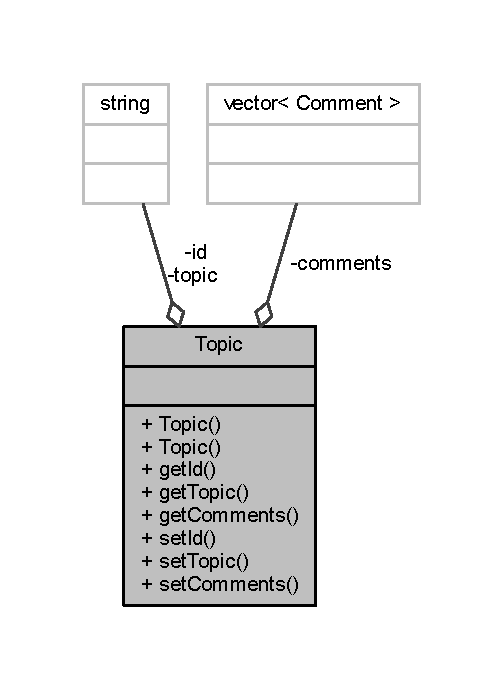
\includegraphics[width=242pt]{class_topic__coll__graph}
\end{center}
\end{figure}
\subsection*{Public Member Functions}
\begin{DoxyCompactItemize}
\item 
\hyperlink{class_topic_af3301cb0d535eb066a3ea4ed54e28414}{Topic} ()
\item 
\hyperlink{class_topic_a1f896499cd9eddcf5138830364860534}{Topic} (std\+::string n\+Id, std\+::string n\+Topic, std\+::vector$<$ \hyperlink{class_comment}{Comment} $>$ n\+Comments)
\item 
std\+::string \hyperlink{class_topic_a0306b941698e573841540d44de1a908a}{get\+Id} ()
\item 
std\+::string \hyperlink{class_topic_a9f6ad6642112c5f121a92aceb8df9c43}{get\+Topic} ()
\item 
std\+::vector$<$ \hyperlink{class_comment}{Comment} $>$ \hyperlink{class_topic_ac800190b0f4f8ee514255cc75bce1f13}{get\+Comments} ()
\item 
void \hyperlink{class_topic_a11ecfa79333a902a33398ac628280cfa}{set\+Id} (std\+::string n\+Id)
\item 
void \hyperlink{class_topic_a64ecaea143938ef771830f05b703853f}{set\+Topic} (std\+::string n\+Topic)
\item 
void \hyperlink{class_topic_ada5f53077553db0022f528b0328a7437}{set\+Comments} (std\+::vector$<$ \hyperlink{class_comment}{Comment} $>$ n\+Comments)
\end{DoxyCompactItemize}
\subsection*{Private Attributes}
\begin{DoxyCompactItemize}
\item 
std\+::string \hyperlink{class_topic_a3f0e95d8c647b06bd9a3e257d86e021a}{id}
\item 
std\+::string \hyperlink{class_topic_ae74abf3428c3d51f0e3c95e995d29633}{topic}
\item 
std\+::vector$<$ \hyperlink{class_comment}{Comment} $>$ \hyperlink{class_topic_a7302f2cd0169b84d3e4e58af7bc1f73d}{comments}
\end{DoxyCompactItemize}
\subsection*{Friends}
\begin{DoxyCompactItemize}
\item 
bool \hyperlink{class_topic_adc7b3e2ce62c70f0ea7a2dcb1649bd24}{operator==} (const \hyperlink{class_topic}{Topic} \&c1, const \hyperlink{class_topic}{Topic} \&c2)
\end{DoxyCompactItemize}


\subsection{Detailed Description}
Model representation for the comment object within the program 

Definition at line 6 of file Topic.\+h.



\subsection{Constructor \& Destructor Documentation}
\mbox{\Hypertarget{class_topic_af3301cb0d535eb066a3ea4ed54e28414}\label{class_topic_af3301cb0d535eb066a3ea4ed54e28414}} 
\index{Topic@{Topic}!Topic@{Topic}}
\index{Topic@{Topic}!Topic@{Topic}}
\subsubsection{\texorpdfstring{Topic()}{Topic()}\hspace{0.1cm}{\footnotesize\ttfamily [1/2]}}
{\footnotesize\ttfamily Topic\+::\+Topic (\begin{DoxyParamCaption}{ }\end{DoxyParamCaption})}



Definition at line 3 of file Topic.\+cpp.


\begin{DoxyCode}
4 \{
5 
6 \}
\end{DoxyCode}
\mbox{\Hypertarget{class_topic_a1f896499cd9eddcf5138830364860534}\label{class_topic_a1f896499cd9eddcf5138830364860534}} 
\index{Topic@{Topic}!Topic@{Topic}}
\index{Topic@{Topic}!Topic@{Topic}}
\subsubsection{\texorpdfstring{Topic()}{Topic()}\hspace{0.1cm}{\footnotesize\ttfamily [2/2]}}
{\footnotesize\ttfamily Topic\+::\+Topic (\begin{DoxyParamCaption}\item[{std\+::string}]{n\+Id,  }\item[{std\+::string}]{n\+Topic,  }\item[{std\+::vector$<$ \hyperlink{class_comment}{Comment} $>$}]{n\+Comments }\end{DoxyParamCaption})}



Definition at line 8 of file Topic.\+cpp.



References set\+Comments(), set\+Id(), and set\+Topic().


\begin{DoxyCode}
9 \{
10     \hyperlink{class_topic_a11ecfa79333a902a33398ac628280cfa}{setId}(nId);
11     \hyperlink{class_topic_a64ecaea143938ef771830f05b703853f}{setTopic}(nTopic);
12     \hyperlink{class_topic_ada5f53077553db0022f528b0328a7437}{setComments}(nComments);
13 \}
\end{DoxyCode}


\subsection{Member Function Documentation}
\mbox{\Hypertarget{class_topic_ac800190b0f4f8ee514255cc75bce1f13}\label{class_topic_ac800190b0f4f8ee514255cc75bce1f13}} 
\index{Topic@{Topic}!get\+Comments@{get\+Comments}}
\index{get\+Comments@{get\+Comments}!Topic@{Topic}}
\subsubsection{\texorpdfstring{get\+Comments()}{getComments()}}
{\footnotesize\ttfamily std\+::vector$<$ \hyperlink{class_comment}{Comment} $>$ Topic\+::get\+Comments (\begin{DoxyParamCaption}{ }\end{DoxyParamCaption})}



Definition at line 25 of file Topic.\+cpp.



References comments.



Referenced by Base\+\_\+\+Group\+::\+Base\+\_\+\+Group().


\begin{DoxyCode}
26 \{
27     \textcolor{keywordflow}{return} \hyperlink{class_topic_a7302f2cd0169b84d3e4e58af7bc1f73d}{comments};
28 \}
\end{DoxyCode}
\mbox{\Hypertarget{class_topic_a0306b941698e573841540d44de1a908a}\label{class_topic_a0306b941698e573841540d44de1a908a}} 
\index{Topic@{Topic}!get\+Id@{get\+Id}}
\index{get\+Id@{get\+Id}!Topic@{Topic}}
\subsubsection{\texorpdfstring{get\+Id()}{getId()}}
{\footnotesize\ttfamily std\+::string Topic\+::get\+Id (\begin{DoxyParamCaption}{ }\end{DoxyParamCaption})}



Definition at line 15 of file Topic.\+cpp.



References id.


\begin{DoxyCode}
16 \{
17     \textcolor{keywordflow}{return} \hyperlink{class_topic_a3f0e95d8c647b06bd9a3e257d86e021a}{id};
18 \}
\end{DoxyCode}
\mbox{\Hypertarget{class_topic_a9f6ad6642112c5f121a92aceb8df9c43}\label{class_topic_a9f6ad6642112c5f121a92aceb8df9c43}} 
\index{Topic@{Topic}!get\+Topic@{get\+Topic}}
\index{get\+Topic@{get\+Topic}!Topic@{Topic}}
\subsubsection{\texorpdfstring{get\+Topic()}{getTopic()}}
{\footnotesize\ttfamily std\+::string Topic\+::get\+Topic (\begin{DoxyParamCaption}{ }\end{DoxyParamCaption})}



Definition at line 20 of file Topic.\+cpp.



References topic.



Referenced by Base\+\_\+\+Group\+::\+Base\+\_\+\+Group().


\begin{DoxyCode}
21 \{
22     \textcolor{keywordflow}{return} \hyperlink{class_topic_ae74abf3428c3d51f0e3c95e995d29633}{topic};
23 \}
\end{DoxyCode}
\mbox{\Hypertarget{class_topic_ada5f53077553db0022f528b0328a7437}\label{class_topic_ada5f53077553db0022f528b0328a7437}} 
\index{Topic@{Topic}!set\+Comments@{set\+Comments}}
\index{set\+Comments@{set\+Comments}!Topic@{Topic}}
\subsubsection{\texorpdfstring{set\+Comments()}{setComments()}}
{\footnotesize\ttfamily void Topic\+::set\+Comments (\begin{DoxyParamCaption}\item[{std\+::vector$<$ \hyperlink{class_comment}{Comment} $>$}]{n\+Comments }\end{DoxyParamCaption})}



Definition at line 40 of file Topic.\+cpp.



Referenced by Topic().


\begin{DoxyCode}
41 \{
42     \hyperlink{namespacecomments}{comments} = nComments;
43 \}
\end{DoxyCode}
\mbox{\Hypertarget{class_topic_a11ecfa79333a902a33398ac628280cfa}\label{class_topic_a11ecfa79333a902a33398ac628280cfa}} 
\index{Topic@{Topic}!set\+Id@{set\+Id}}
\index{set\+Id@{set\+Id}!Topic@{Topic}}
\subsubsection{\texorpdfstring{set\+Id()}{setId()}}
{\footnotesize\ttfamily void Topic\+::set\+Id (\begin{DoxyParamCaption}\item[{std\+::string}]{n\+Id }\end{DoxyParamCaption})}



Definition at line 30 of file Topic.\+cpp.



Referenced by Topic().


\begin{DoxyCode}
31 \{
32     \textcolor{keywordtype}{id} = nId;
33 \}
\end{DoxyCode}
\mbox{\Hypertarget{class_topic_a64ecaea143938ef771830f05b703853f}\label{class_topic_a64ecaea143938ef771830f05b703853f}} 
\index{Topic@{Topic}!set\+Topic@{set\+Topic}}
\index{set\+Topic@{set\+Topic}!Topic@{Topic}}
\subsubsection{\texorpdfstring{set\+Topic()}{setTopic()}}
{\footnotesize\ttfamily void Topic\+::set\+Topic (\begin{DoxyParamCaption}\item[{std\+::string}]{n\+Topic }\end{DoxyParamCaption})}



Definition at line 35 of file Topic.\+cpp.



References topic.



Referenced by Topic().


\begin{DoxyCode}
36 \{
37     \hyperlink{class_topic_ae74abf3428c3d51f0e3c95e995d29633}{topic} = nTopic;
38 \}
\end{DoxyCode}


\subsection{Friends And Related Function Documentation}
\mbox{\Hypertarget{class_topic_adc7b3e2ce62c70f0ea7a2dcb1649bd24}\label{class_topic_adc7b3e2ce62c70f0ea7a2dcb1649bd24}} 
\index{Topic@{Topic}!operator==@{operator==}}
\index{operator==@{operator==}!Topic@{Topic}}
\subsubsection{\texorpdfstring{operator==}{operator==}}
{\footnotesize\ttfamily bool operator== (\begin{DoxyParamCaption}\item[{const \hyperlink{class_topic}{Topic} \&}]{c1,  }\item[{const \hyperlink{class_topic}{Topic} \&}]{c2 }\end{DoxyParamCaption})\hspace{0.3cm}{\ttfamily [friend]}}



Definition at line 45 of file Topic.\+cpp.


\begin{DoxyCode}
46 \{
47     \textcolor{keywordflow}{return}  (t1.id == t2.id) && (t1.topic == t2.topic) && (t1.comments == t2.comments);
48 \}
\end{DoxyCode}


\subsection{Member Data Documentation}
\mbox{\Hypertarget{class_topic_a7302f2cd0169b84d3e4e58af7bc1f73d}\label{class_topic_a7302f2cd0169b84d3e4e58af7bc1f73d}} 
\index{Topic@{Topic}!comments@{comments}}
\index{comments@{comments}!Topic@{Topic}}
\subsubsection{\texorpdfstring{comments}{comments}}
{\footnotesize\ttfamily std\+::vector$<$\hyperlink{class_comment}{Comment}$>$ Topic\+::comments\hspace{0.3cm}{\ttfamily [private]}}



Definition at line 22 of file Topic.\+h.



Referenced by get\+Comments(), and operator==().

\mbox{\Hypertarget{class_topic_a3f0e95d8c647b06bd9a3e257d86e021a}\label{class_topic_a3f0e95d8c647b06bd9a3e257d86e021a}} 
\index{Topic@{Topic}!id@{id}}
\index{id@{id}!Topic@{Topic}}
\subsubsection{\texorpdfstring{id}{id}}
{\footnotesize\ttfamily std\+::string Topic\+::id\hspace{0.3cm}{\ttfamily [private]}}



Definition at line 20 of file Topic.\+h.



Referenced by get\+Id(), and operator==().

\mbox{\Hypertarget{class_topic_ae74abf3428c3d51f0e3c95e995d29633}\label{class_topic_ae74abf3428c3d51f0e3c95e995d29633}} 
\index{Topic@{Topic}!topic@{topic}}
\index{topic@{topic}!Topic@{Topic}}
\subsubsection{\texorpdfstring{topic}{topic}}
{\footnotesize\ttfamily std\+::string Topic\+::topic\hspace{0.3cm}{\ttfamily [private]}}



Definition at line 21 of file Topic.\+h.



Referenced by get\+Topic(), operator==(), and set\+Topic().



The documentation for this class was generated from the following files\+:\begin{DoxyCompactItemize}
\item 
C\+:/\+Users/\+Kyle Tuckey/\+Documents/\+Final Year Project/\+Social\+\_\+\+N\+P\+C\+S/\+Social\+\_\+\+N\+P\+C\+S/\hyperlink{_topic_8h}{Topic.\+h}\item 
C\+:/\+Users/\+Kyle Tuckey/\+Documents/\+Final Year Project/\+Social\+\_\+\+N\+P\+C\+S/\+Social\+\_\+\+N\+P\+C\+S/\hyperlink{_topic_8cpp}{Topic.\+cpp}\end{DoxyCompactItemize}

\hypertarget{class_user___group}{}\section{User\+\_\+\+Group Class Reference}
\label{class_user___group}\index{User\+\_\+\+Group@{User\+\_\+\+Group}}


{\ttfamily \#include $<$User\+\_\+\+Group.\+h$>$}



Inheritance diagram for User\+\_\+\+Group\+:\nopagebreak
\begin{figure}[H]
\begin{center}
\leavevmode
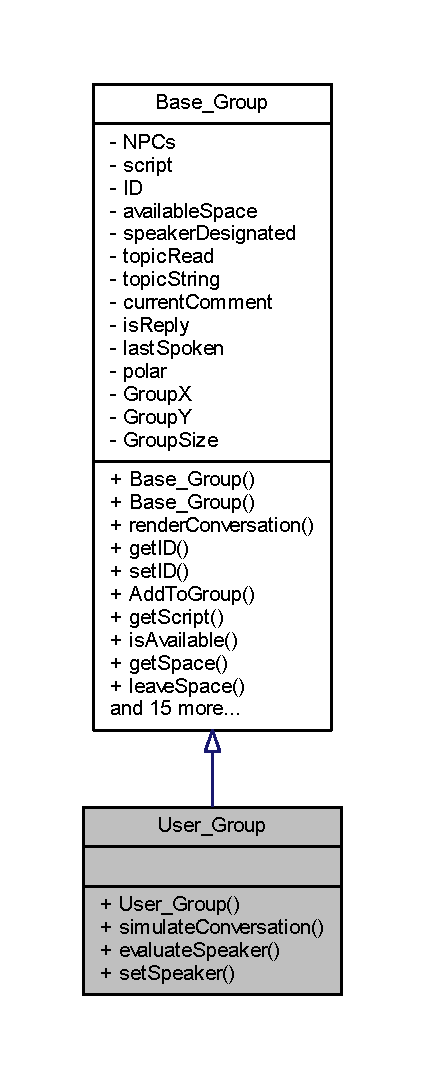
\includegraphics[width=204pt]{class_user___group__inherit__graph}
\end{center}
\end{figure}


Collaboration diagram for User\+\_\+\+Group\+:\nopagebreak
\begin{figure}[H]
\begin{center}
\leavevmode
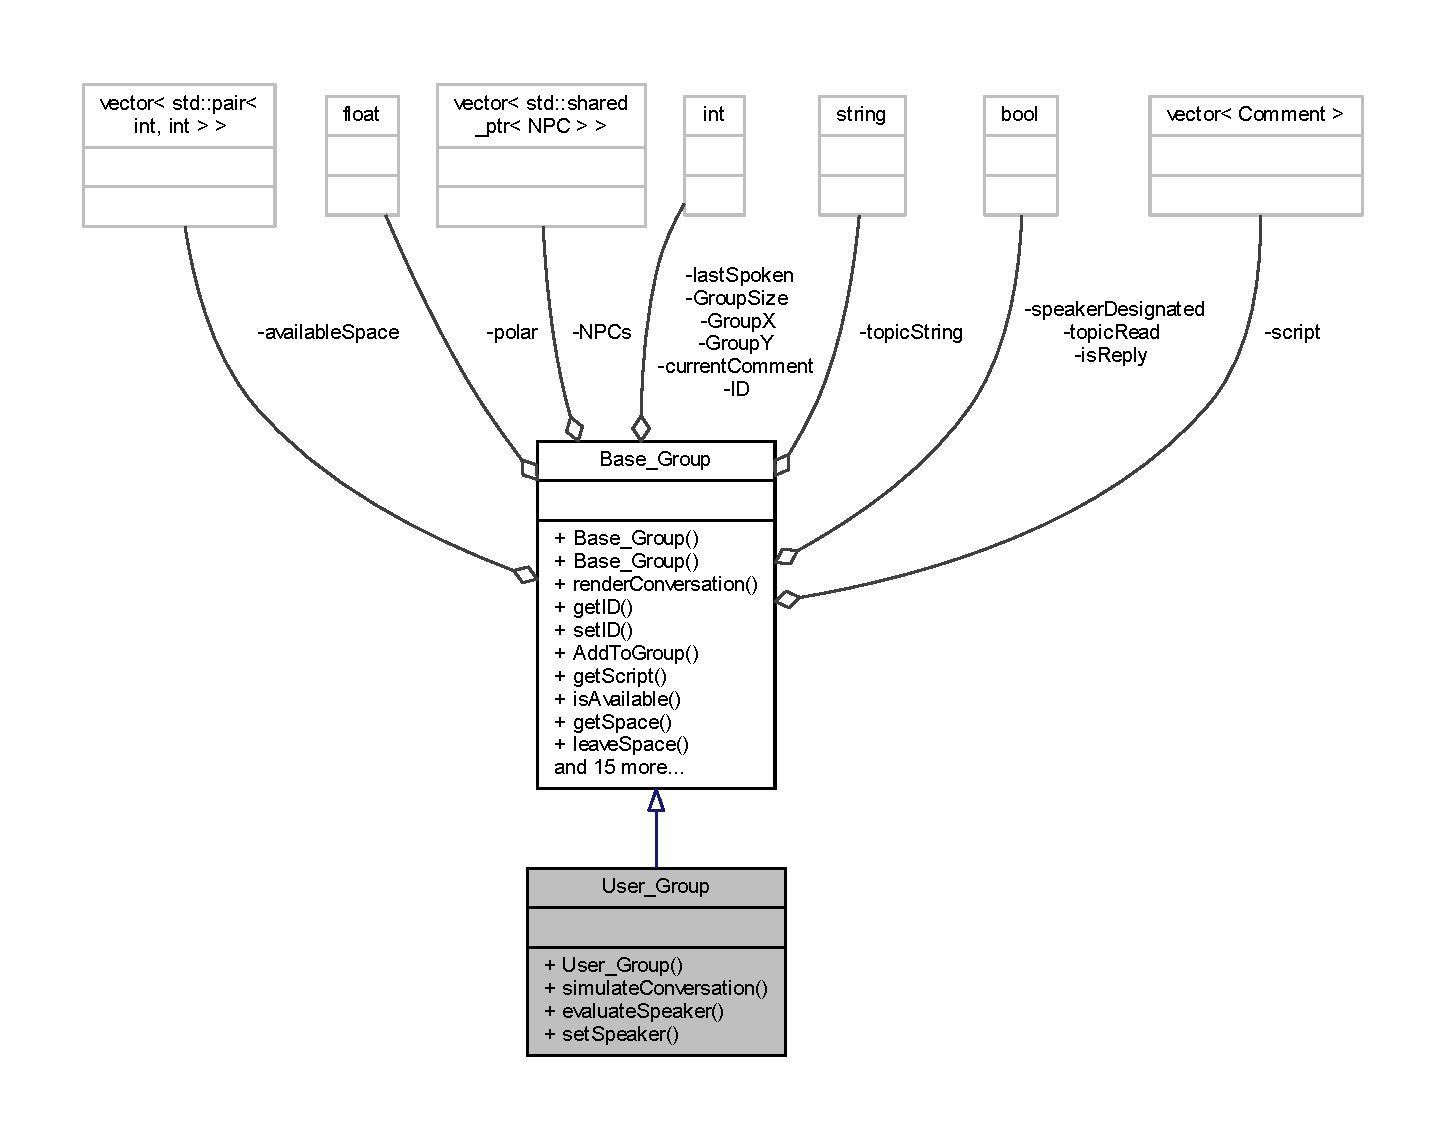
\includegraphics[width=350pt]{class_user___group__coll__graph}
\end{center}
\end{figure}
\subsection*{Public Member Functions}
\begin{DoxyCompactItemize}
\item 
\hyperlink{class_user___group_a553bb5b748ef79772fe5cecedc2154be}{User\+\_\+\+Group} (int x, int y, int size, std\+::string t\+Box\+File, std\+::string npc\+File, S\+D\+L\+\_\+\+Renderer $\ast$renderer, \hyperlink{class_topic}{Topic} tp)
\item 
void \hyperlink{class_user___group_a0142ca8121ea4bb4d881153e48e486f9}{simulate\+Conversation} (S\+D\+L\+\_\+\+Renderer $\ast$renderer, bool time, std\+::string boredom\+Level, T\+T\+F\+\_\+\+Font $\ast$font)
\begin{DoxyCompactList}\small\item\em Template methods to be inherited by child classes, these are the core classes for simulating conversation. \end{DoxyCompactList}\item 
bool \hyperlink{class_user___group_a40051b822a0f0dd126b95d0f0fd28eff}{evaluate\+Speaker} ()
\item 
void \hyperlink{class_user___group_aeb67757a4645ae32ea0b9c426fece2de}{set\+Speaker} (std\+::string boredom\+Level)
\end{DoxyCompactItemize}


\subsection{Detailed Description}


Definition at line 4 of file User\+\_\+\+Group.\+h.



\subsection{Constructor \& Destructor Documentation}
\mbox{\Hypertarget{class_user___group_a553bb5b748ef79772fe5cecedc2154be}\label{class_user___group_a553bb5b748ef79772fe5cecedc2154be}} 
\index{User\+\_\+\+Group@{User\+\_\+\+Group}!User\+\_\+\+Group@{User\+\_\+\+Group}}
\index{User\+\_\+\+Group@{User\+\_\+\+Group}!User\+\_\+\+Group@{User\+\_\+\+Group}}
\subsubsection{\texorpdfstring{User\+\_\+\+Group()}{User\_Group()}}
{\footnotesize\ttfamily User\+\_\+\+Group\+::\+User\+\_\+\+Group (\begin{DoxyParamCaption}\item[{int}]{x,  }\item[{int}]{y,  }\item[{int}]{size,  }\item[{std\+::string}]{t\+Box\+File,  }\item[{std\+::string}]{npc\+File,  }\item[{S\+D\+L\+\_\+\+Renderer $\ast$}]{renderer,  }\item[{\hyperlink{class_topic}{Topic}}]{tp }\end{DoxyParamCaption})}



Definition at line 5 of file User\+\_\+\+Group.\+cpp.


\begin{DoxyCode}
5                                                                                                            
                : \hyperlink{class_base___group_a96e70ee101d6430696f7b13b07190787}{Base\_Group}(x, y, size, tBoxFile, npcFile, renderer, tp)
6 \{\}
\end{DoxyCode}


\subsection{Member Function Documentation}
\mbox{\Hypertarget{class_user___group_a40051b822a0f0dd126b95d0f0fd28eff}\label{class_user___group_a40051b822a0f0dd126b95d0f0fd28eff}} 
\index{User\+\_\+\+Group@{User\+\_\+\+Group}!evaluate\+Speaker@{evaluate\+Speaker}}
\index{evaluate\+Speaker@{evaluate\+Speaker}!User\+\_\+\+Group@{User\+\_\+\+Group}}
\subsubsection{\texorpdfstring{evaluate\+Speaker()}{evaluateSpeaker()}}
{\footnotesize\ttfamily bool User\+\_\+\+Group\+::evaluate\+Speaker (\begin{DoxyParamCaption}{ }\end{DoxyParamCaption})\hspace{0.3cm}{\ttfamily [virtual]}}



Reimplemented from \hyperlink{class_base___group_a8264ff598ce7e789c6419e2e6eef08fd}{Base\+\_\+\+Group}.



Definition at line 13 of file User\+\_\+\+Group.\+cpp.



References Base\+\_\+\+Group\+::get\+N\+P\+C\+List(), and Base\+\_\+\+Group\+::\+N\+P\+Cs.



Referenced by set\+Speaker().


\begin{DoxyCode}
14 \{
15     std::vector<std::shared\_ptr<NPC>> \hyperlink{class_base___group_a4757f3c06c73eea029f71b871c1d863e}{NPCs} = \hyperlink{class_base___group_a75eec9132aaf532b4429e0af76b31775}{getNPCList}();
16     \textcolor{keywordflow}{for} (\textcolor{keywordtype}{int} i = 0; i < NPCs.size(); i++)
17     \{
18         \textcolor{keywordflow}{if} (NPCs[i]->getSpeaking())
19             \textcolor{keywordflow}{return} \textcolor{keyword}{true};
20     \}
21     \textcolor{keywordflow}{return} \textcolor{keyword}{false};
22 \}
\end{DoxyCode}
\mbox{\Hypertarget{class_user___group_aeb67757a4645ae32ea0b9c426fece2de}\label{class_user___group_aeb67757a4645ae32ea0b9c426fece2de}} 
\index{User\+\_\+\+Group@{User\+\_\+\+Group}!set\+Speaker@{set\+Speaker}}
\index{set\+Speaker@{set\+Speaker}!User\+\_\+\+Group@{User\+\_\+\+Group}}
\subsubsection{\texorpdfstring{set\+Speaker()}{setSpeaker()}}
{\footnotesize\ttfamily void User\+\_\+\+Group\+::set\+Speaker (\begin{DoxyParamCaption}\item[{std\+::string}]{boredom\+Level }\end{DoxyParamCaption})\hspace{0.3cm}{\ttfamily [virtual]}}



Reimplemented from \hyperlink{class_base___group_ae35b3719076cf40d6577b4ae3779758c}{Base\+\_\+\+Group}.



Definition at line 24 of file User\+\_\+\+Group.\+cpp.



References evaluate\+Speaker(), Base\+\_\+\+Group\+::get\+I\+D(), Base\+\_\+\+Group\+::get\+N\+P\+C\+List(), Base\+\_\+\+Group\+::\+Get\+Random\+Number(), Base\+\_\+\+Group\+::get\+Script(), and Base\+\_\+\+Group\+::\+N\+P\+Cs.


\begin{DoxyCode}
25 \{
26     \textcolor{keywordflow}{if} (!\hyperlink{class_user___group_a40051b822a0f0dd126b95d0f0fd28eff}{evaluateSpeaker}()) \{
27         \textcolor{keywordtype}{int} r = \hyperlink{class_base___group_a3864a2806457151363344051f2814389}{GetRandomNumber}();
28         std::vector<std::shared\_ptr<NPC>> \hyperlink{class_base___group_a4757f3c06c73eea029f71b871c1d863e}{NPCs} = \hyperlink{class_base___group_a75eec9132aaf532b4429e0af76b31775}{getNPCList}();
29         std::vector<Comment> comms = \hyperlink{class_base___group_a48dadfbc8cdefca9bdd2c42b99115ad8}{getScript}();
30         \textcolor{keywordflow}{for} (\textcolor{keywordtype}{int} i = 0; i < NPCs.size(); i++)
31         \{
32             \textcolor{keywordflow}{if} (NPCs[i]->\hyperlink{class_base___group_a7299ae154b26d741ac2f6f794bc3a544}{getID}() != NPCs[r]->getID())
33             \{
34                 std::string pred = NPCs[i]->getCurrentUser();
35                 \textcolor{comment}{/*}
36 \textcolor{comment}{                if (std::find\_if(comms.begin(), comms.end(), CommentComp(pred)) != comms.end())}
37 \textcolor{comment}{                \{}
38 \textcolor{comment}{}
39 \textcolor{comment}{                \};}
40 \textcolor{comment}{                */}
41             \}
42         \}
43         NPCs[r]->setSpeaking(\textcolor{keyword}{true});
44     \}
45 \}
\end{DoxyCode}
\mbox{\Hypertarget{class_user___group_a0142ca8121ea4bb4d881153e48e486f9}\label{class_user___group_a0142ca8121ea4bb4d881153e48e486f9}} 
\index{User\+\_\+\+Group@{User\+\_\+\+Group}!simulate\+Conversation@{simulate\+Conversation}}
\index{simulate\+Conversation@{simulate\+Conversation}!User\+\_\+\+Group@{User\+\_\+\+Group}}
\subsubsection{\texorpdfstring{simulate\+Conversation()}{simulateConversation()}}
{\footnotesize\ttfamily void User\+\_\+\+Group\+::simulate\+Conversation (\begin{DoxyParamCaption}\item[{S\+D\+L\+\_\+\+Renderer $\ast$}]{renderer,  }\item[{bool}]{time,  }\item[{std\+::string}]{boredom\+Level,  }\item[{T\+T\+F\+\_\+\+Font $\ast$}]{font }\end{DoxyParamCaption})\hspace{0.3cm}{\ttfamily [virtual]}}



Template methods to be inherited by child classes, these are the core classes for simulating conversation. 



Reimplemented from \hyperlink{class_base___group_aa5080b6388c5974394bf326ce80bfa91}{Base\+\_\+\+Group}.



Definition at line 8 of file User\+\_\+\+Group.\+cpp.


\begin{DoxyCode}
9 \{
10     \textcolor{comment}{// TODO: implement algorithm 2}
11 \}
\end{DoxyCode}


The documentation for this class was generated from the following files\+:\begin{DoxyCompactItemize}
\item 
C\+:/\+Users/\+Kyle Tuckey/\+Documents/\+Final Year Project/\+Social\+\_\+\+N\+P\+C\+S/\+Social\+\_\+\+N\+P\+C\+S/\hyperlink{_user___group_8h}{User\+\_\+\+Group.\+h}\item 
C\+:/\+Users/\+Kyle Tuckey/\+Documents/\+Final Year Project/\+Social\+\_\+\+N\+P\+C\+S/\+Social\+\_\+\+N\+P\+C\+S/\hyperlink{_user___group_8cpp}{User\+\_\+\+Group.\+cpp}\end{DoxyCompactItemize}

\chapter{File Documentation}
\hypertarget{_base___group_8cpp}{}\section{C\+:/\+Users/\+Kyle Tuckey/\+Documents/\+Final Year Project/\+Social\+\_\+\+N\+P\+C\+S/\+Social\+\_\+\+N\+P\+C\+S/\+Base\+\_\+\+Group.cpp File Reference}
\label{_base___group_8cpp}\index{C\+:/\+Users/\+Kyle Tuckey/\+Documents/\+Final Year Project/\+Social\+\_\+\+N\+P\+C\+S/\+Social\+\_\+\+N\+P\+C\+S/\+Base\+\_\+\+Group.\+cpp@{C\+:/\+Users/\+Kyle Tuckey/\+Documents/\+Final Year Project/\+Social\+\_\+\+N\+P\+C\+S/\+Social\+\_\+\+N\+P\+C\+S/\+Base\+\_\+\+Group.\+cpp}}


base class for the \hyperlink{class_n_p_c}{N\+PC} group classes The \hyperlink{class_n_p_c___group}{N\+P\+C\+\_\+\+Group} class is designed to represent a maximum group of 6 \hyperlink{class_n_p_c}{N\+PC}\textquotesingle{}s. the specfied \hyperlink{class_n_p_c}{N\+PC}\textquotesingle{}s are initialised when the group is initialised.  


{\ttfamily \#include \char`\"{}Base\+\_\+\+Group.\+h\char`\"{}}\newline
Include dependency graph for Base\+\_\+\+Group.\+cpp\+:\nopagebreak
\begin{figure}[H]
\begin{center}
\leavevmode
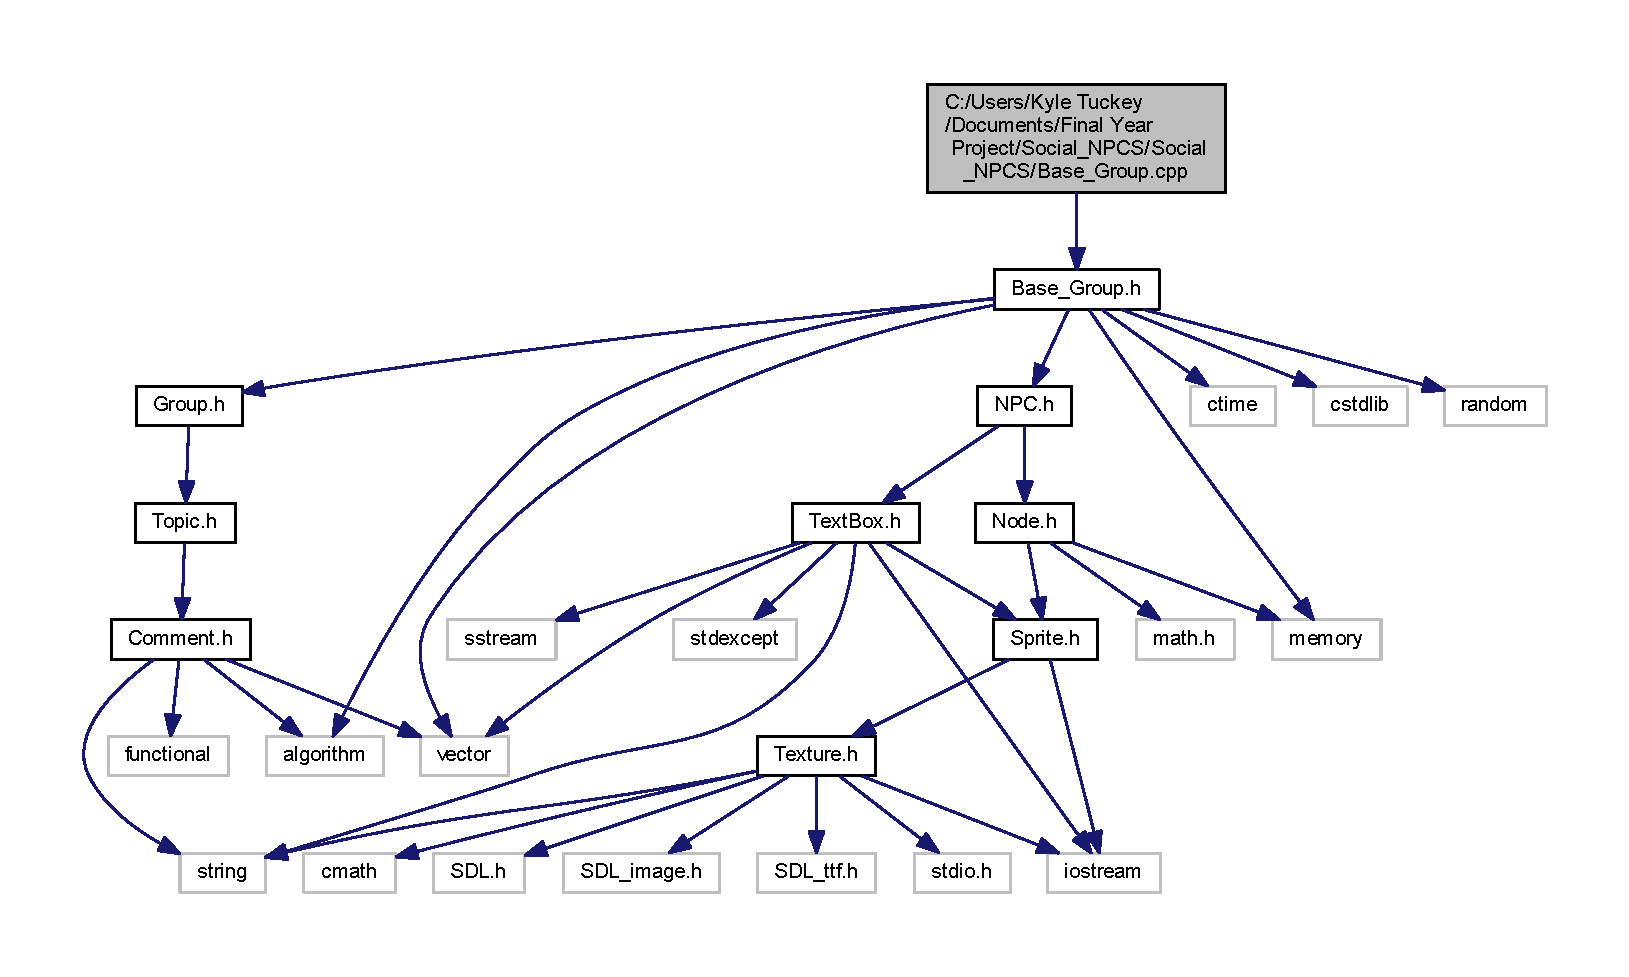
\includegraphics[width=350pt]{_base___group_8cpp__incl}
\end{center}
\end{figure}


\subsection{Detailed Description}
base class for the \hyperlink{class_n_p_c}{N\+PC} group classes The \hyperlink{class_n_p_c___group}{N\+P\+C\+\_\+\+Group} class is designed to represent a maximum group of 6 \hyperlink{class_n_p_c}{N\+PC}\textquotesingle{}s. the specfied \hyperlink{class_n_p_c}{N\+PC}\textquotesingle{}s are initialised when the group is initialised. 


\hypertarget{_base___group_8h}{}\section{C\+:/\+Users/\+Kyle Tuckey/\+Documents/\+Final Year Project/\+Social\+\_\+\+N\+P\+C\+S/\+Social\+\_\+\+N\+P\+C\+S/\+Base\+\_\+\+Group.h File Reference}
\label{_base___group_8h}\index{C\+:/\+Users/\+Kyle Tuckey/\+Documents/\+Final Year Project/\+Social\+\_\+\+N\+P\+C\+S/\+Social\+\_\+\+N\+P\+C\+S/\+Base\+\_\+\+Group.\+h@{C\+:/\+Users/\+Kyle Tuckey/\+Documents/\+Final Year Project/\+Social\+\_\+\+N\+P\+C\+S/\+Social\+\_\+\+N\+P\+C\+S/\+Base\+\_\+\+Group.\+h}}
{\ttfamily \#include $<$vector$>$}\newline
{\ttfamily \#include \char`\"{}N\+P\+C.\+h\char`\"{}}\newline
{\ttfamily \#include \char`\"{}Group.\+h\char`\"{}}\newline
{\ttfamily \#include $<$algorithm$>$}\newline
{\ttfamily \#include $<$ctime$>$}\newline
{\ttfamily \#include $<$cstdlib$>$}\newline
{\ttfamily \#include $<$memory$>$}\newline
{\ttfamily \#include $<$random$>$}\newline
Include dependency graph for Base\+\_\+\+Group.\+h\+:\nopagebreak
\begin{figure}[H]
\begin{center}
\leavevmode
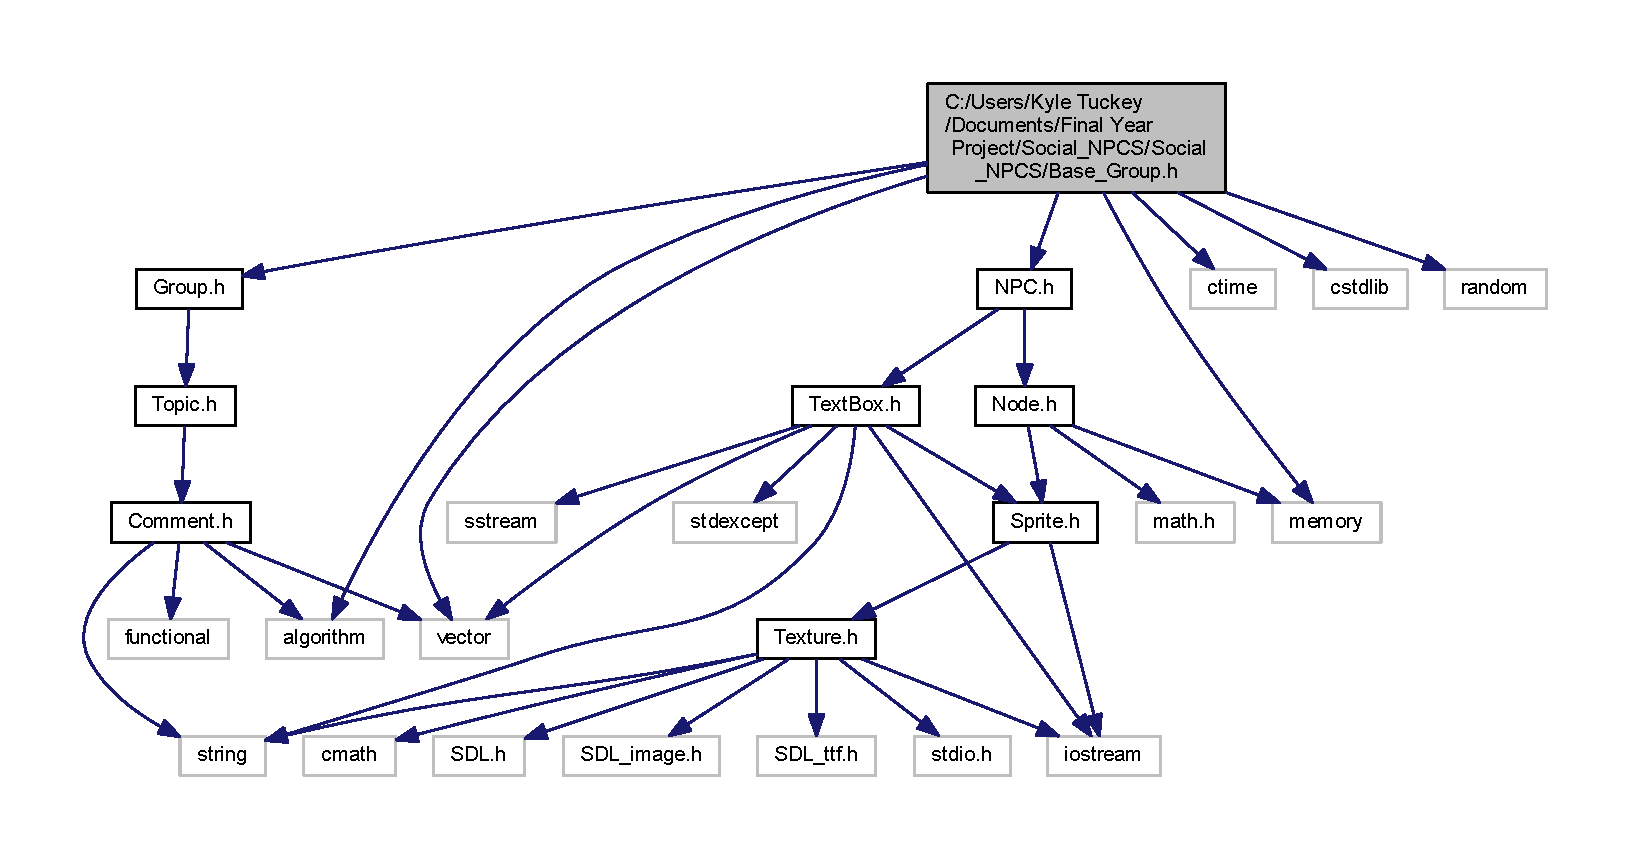
\includegraphics[width=350pt]{_base___group_8h__incl}
\end{center}
\end{figure}
This graph shows which files directly or indirectly include this file\+:\nopagebreak
\begin{figure}[H]
\begin{center}
\leavevmode
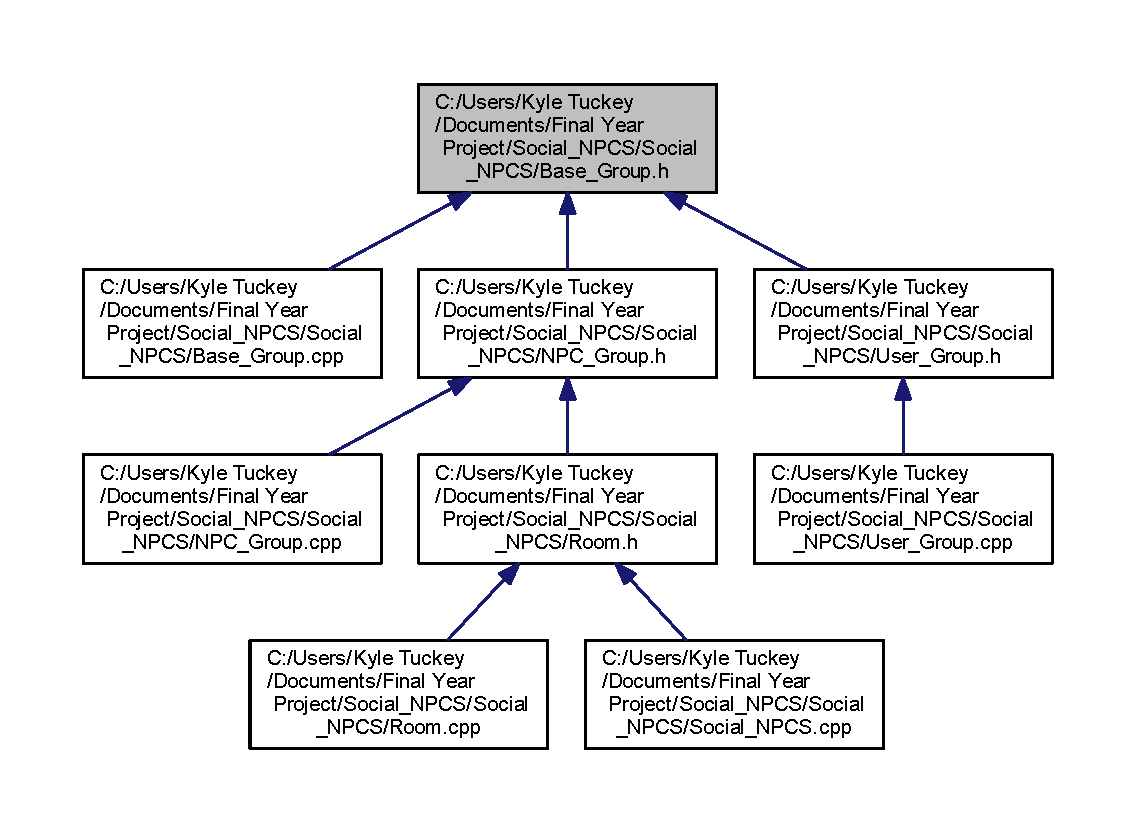
\includegraphics[width=350pt]{_base___group_8h__dep__incl}
\end{center}
\end{figure}
\subsection*{Classes}
\begin{DoxyCompactItemize}
\item 
class \hyperlink{class_base___group}{Base\+\_\+\+Group}
\end{DoxyCompactItemize}

\hypertarget{_comment_8cpp}{}\section{C\+:/\+Users/\+Kyle Tuckey/\+Documents/\+Final Year Project/\+Social\+\_\+\+N\+P\+C\+S/\+Social\+\_\+\+N\+P\+C\+S/\+Comment.cpp File Reference}
\label{_comment_8cpp}\index{C\+:/\+Users/\+Kyle Tuckey/\+Documents/\+Final Year Project/\+Social\+\_\+\+N\+P\+C\+S/\+Social\+\_\+\+N\+P\+C\+S/\+Comment.\+cpp@{C\+:/\+Users/\+Kyle Tuckey/\+Documents/\+Final Year Project/\+Social\+\_\+\+N\+P\+C\+S/\+Social\+\_\+\+N\+P\+C\+S/\+Comment.\+cpp}}
{\ttfamily \#include \char`\"{}Comment.\+h\char`\"{}}\newline
Include dependency graph for Comment.\+cpp\+:\nopagebreak
\begin{figure}[H]
\begin{center}
\leavevmode
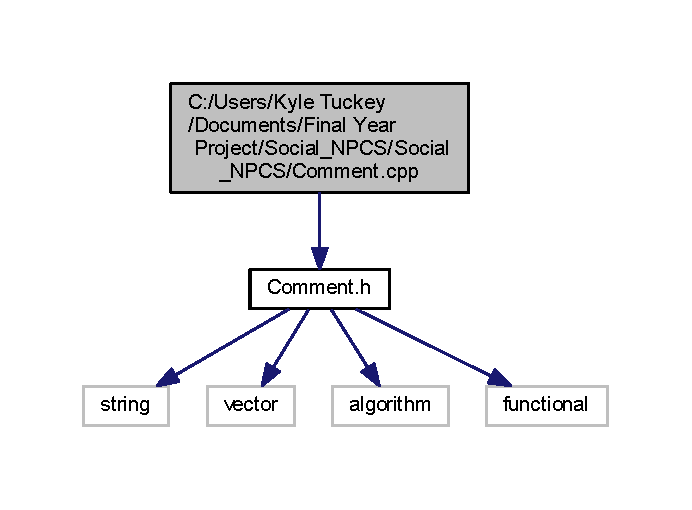
\includegraphics[width=332pt]{_comment_8cpp__incl}
\end{center}
\end{figure}
\subsection*{Functions}
\begin{DoxyCompactItemize}
\item 
bool \hyperlink{_comment_8cpp_ac5edd8dbab6e9d702dcdde889b96c250}{operator==} (const \hyperlink{class_comment}{Comment} \&c1, const \hyperlink{class_comment}{Comment} \&c2)
\end{DoxyCompactItemize}


\subsection{Function Documentation}
\mbox{\Hypertarget{_comment_8cpp_ac5edd8dbab6e9d702dcdde889b96c250}\label{_comment_8cpp_ac5edd8dbab6e9d702dcdde889b96c250}} 
\index{Comment.\+cpp@{Comment.\+cpp}!operator==@{operator==}}
\index{operator==@{operator==}!Comment.\+cpp@{Comment.\+cpp}}
\subsubsection{\texorpdfstring{operator==()}{operator==()}}
{\footnotesize\ttfamily bool operator== (\begin{DoxyParamCaption}\item[{const \hyperlink{class_comment}{Comment} \&}]{c1,  }\item[{const \hyperlink{class_comment}{Comment} \&}]{c2 }\end{DoxyParamCaption})}



Definition at line 66 of file Comment.\+cpp.



References Comment\+::body, Comment\+::id, Comment\+::parent\+\_\+id, Comment\+::polarity, and Comment\+::reply.


\begin{DoxyCode}
67 \{
68     \textcolor{keywordflow}{return} (c1.\hyperlink{class_comment_a63db6067036146247c4ab7f663d90369}{id} == c2.\hyperlink{class_comment_a63db6067036146247c4ab7f663d90369}{id}) && (c1.\hyperlink{class_comment_af8df10ee9d38440d5c4d500ccc9f2519}{body} == c2.\hyperlink{class_comment_af8df10ee9d38440d5c4d500ccc9f2519}{body}) && (c1.\hyperlink{class_comment_abc88c0f64df05cb3d29ad1c7aa1621c5}{parent\_id} == c2.
      \hyperlink{class_comment_abc88c0f64df05cb3d29ad1c7aa1621c5}{parent\_id}) && (c1.\hyperlink{class_comment_a617b67425b39c1f5f1eb0ada3d4bbd74}{polarity} == c2.\hyperlink{class_comment_a617b67425b39c1f5f1eb0ada3d4bbd74}{polarity}) && (c1.\hyperlink{class_comment_a7b8ceeb67364d5e08299baeeff38ba03}{reply} == c2.
      \hyperlink{class_comment_a7b8ceeb67364d5e08299baeeff38ba03}{reply});
69 \}
\end{DoxyCode}

\hypertarget{_comment_8h}{}\section{C\+:/\+Users/\+Kyle Tuckey/\+Documents/\+Final Year Project/\+Social\+\_\+\+N\+P\+C\+S/\+Social\+\_\+\+N\+P\+C\+S/\+Comment.h File Reference}
\label{_comment_8h}\index{C\+:/\+Users/\+Kyle Tuckey/\+Documents/\+Final Year Project/\+Social\+\_\+\+N\+P\+C\+S/\+Social\+\_\+\+N\+P\+C\+S/\+Comment.\+h@{C\+:/\+Users/\+Kyle Tuckey/\+Documents/\+Final Year Project/\+Social\+\_\+\+N\+P\+C\+S/\+Social\+\_\+\+N\+P\+C\+S/\+Comment.\+h}}
{\ttfamily \#include $<$string$>$}\newline
{\ttfamily \#include $<$vector$>$}\newline
{\ttfamily \#include $<$algorithm$>$}\newline
{\ttfamily \#include $<$functional$>$}\newline
Include dependency graph for Comment.\+h\+:\nopagebreak
\begin{figure}[H]
\begin{center}
\leavevmode
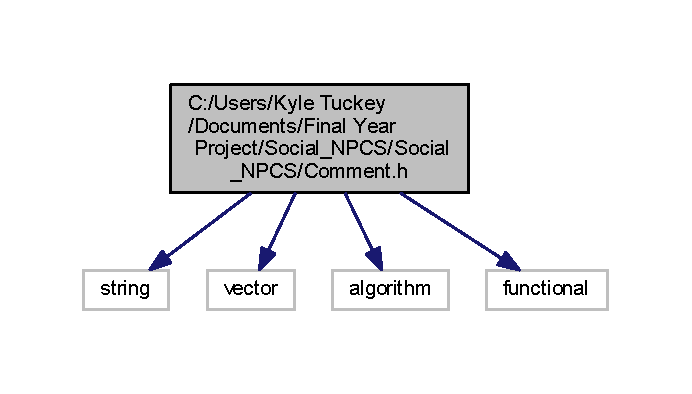
\includegraphics[width=332pt]{_comment_8h__incl}
\end{center}
\end{figure}
This graph shows which files directly or indirectly include this file\+:\nopagebreak
\begin{figure}[H]
\begin{center}
\leavevmode
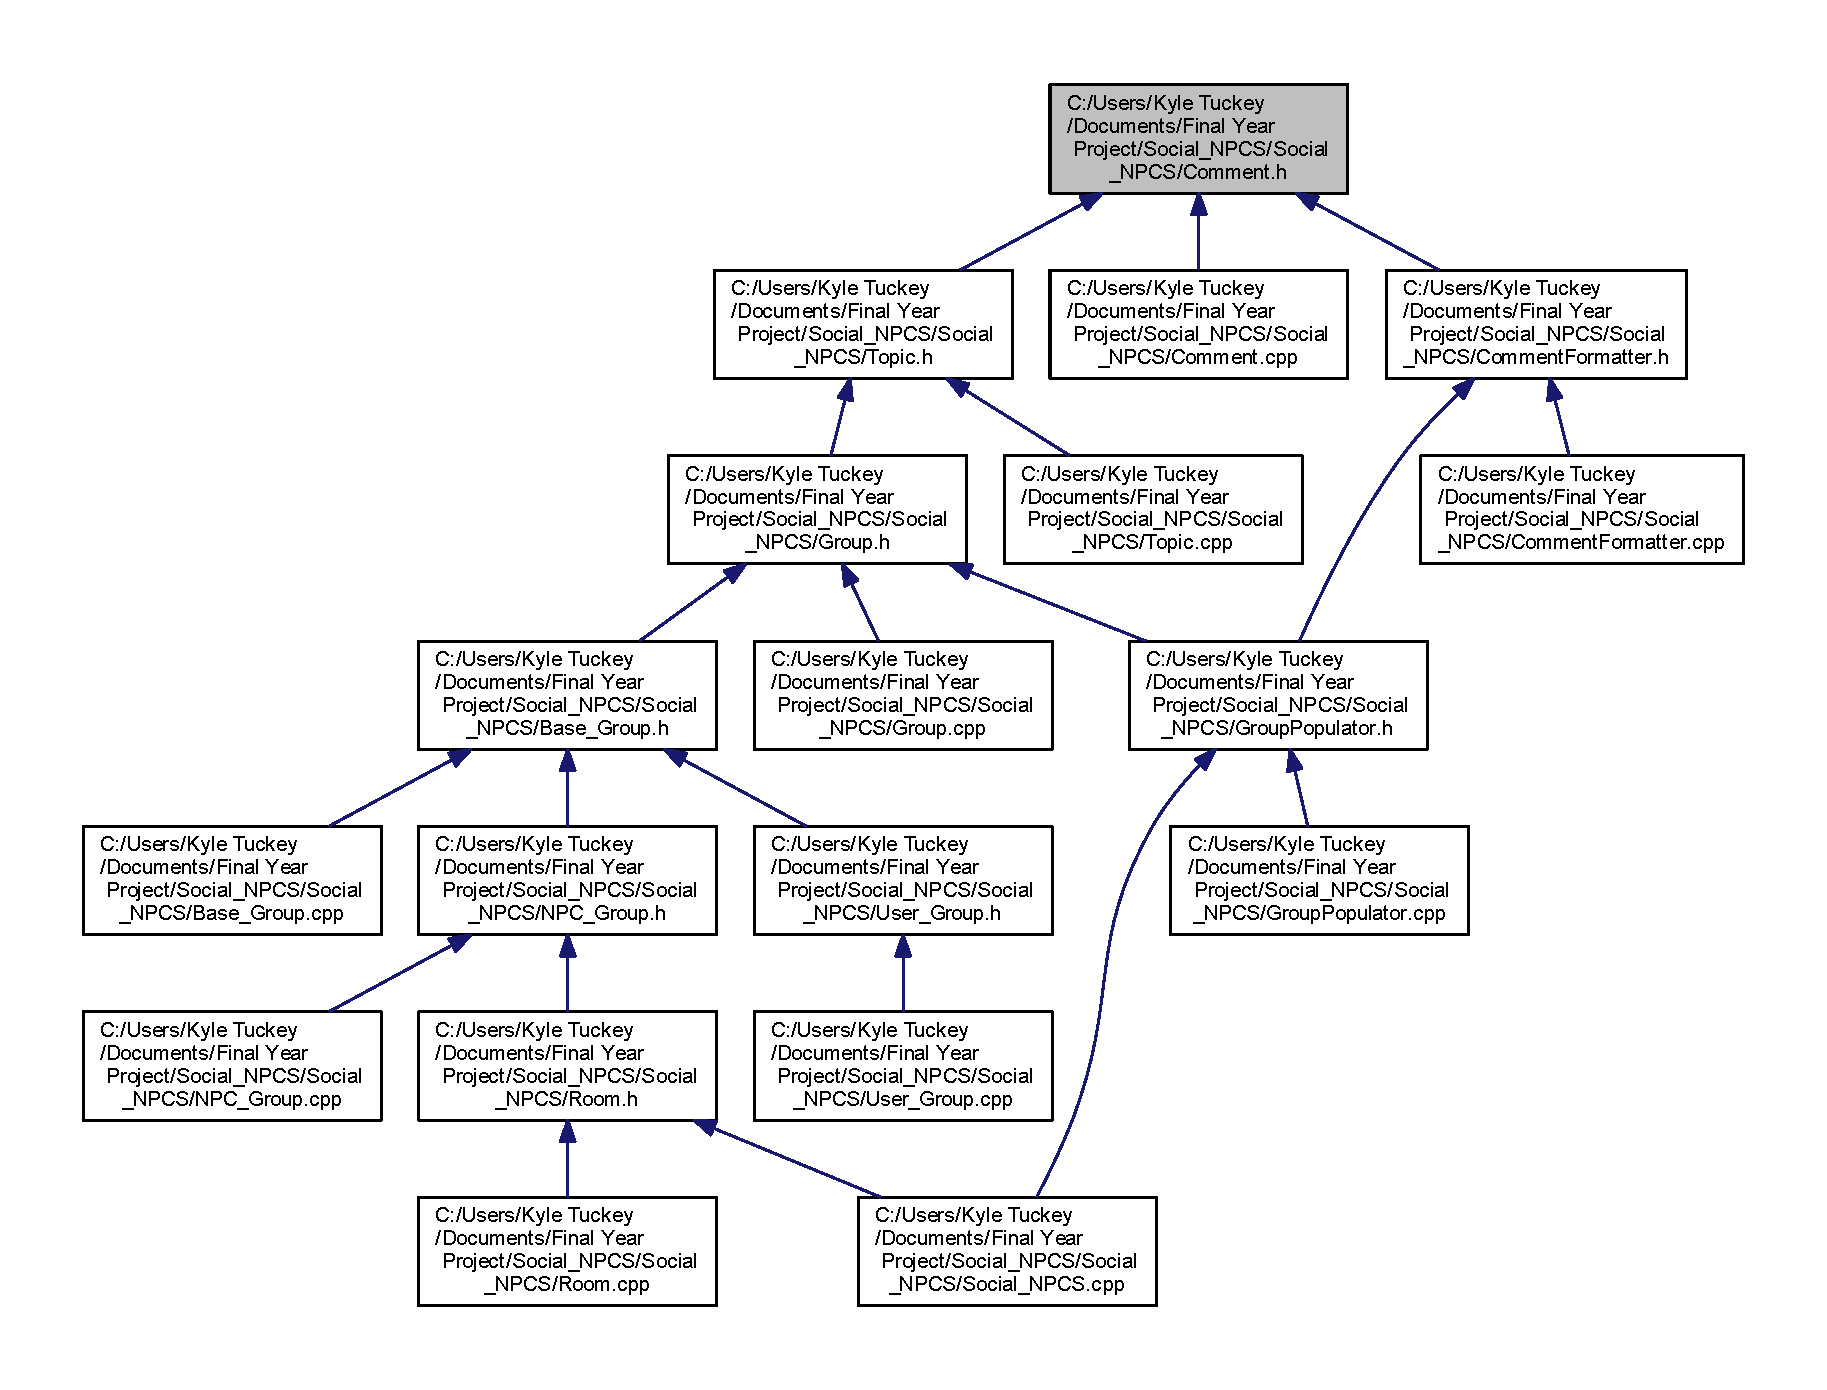
\includegraphics[width=350pt]{_comment_8h__dep__incl}
\end{center}
\end{figure}
\subsection*{Classes}
\begin{DoxyCompactItemize}
\item 
class \hyperlink{class_comment}{Comment}
\end{DoxyCompactItemize}

\hypertarget{_comment_formatter_8cpp}{}\section{C\+:/\+Users/\+Kyle Tuckey/\+Documents/\+Final Year Project/\+Social\+\_\+\+N\+P\+C\+S/\+Social\+\_\+\+N\+P\+C\+S/\+Comment\+Formatter.cpp File Reference}
\label{_comment_formatter_8cpp}\index{C\+:/\+Users/\+Kyle Tuckey/\+Documents/\+Final Year Project/\+Social\+\_\+\+N\+P\+C\+S/\+Social\+\_\+\+N\+P\+C\+S/\+Comment\+Formatter.\+cpp@{C\+:/\+Users/\+Kyle Tuckey/\+Documents/\+Final Year Project/\+Social\+\_\+\+N\+P\+C\+S/\+Social\+\_\+\+N\+P\+C\+S/\+Comment\+Formatter.\+cpp}}
{\ttfamily \#include \char`\"{}Comment\+Formatter.\+h\char`\"{}}\newline
Include dependency graph for Comment\+Formatter.\+cpp\+:\nopagebreak
\begin{figure}[H]
\begin{center}
\leavevmode
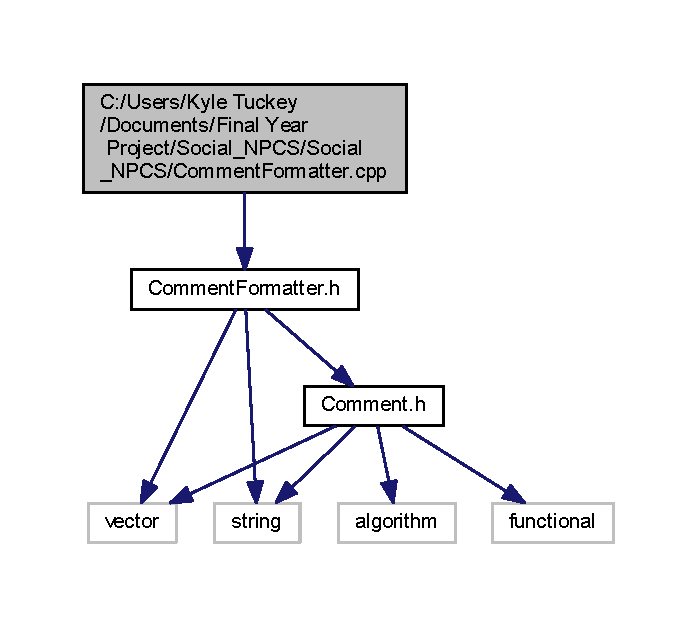
\includegraphics[width=335pt]{_comment_formatter_8cpp__incl}
\end{center}
\end{figure}

\hypertarget{_comment_formatter_8h}{}\section{C\+:/\+Users/\+Kyle Tuckey/\+Documents/\+Final Year Project/\+Social\+\_\+\+N\+P\+C\+S/\+Social\+\_\+\+N\+P\+C\+S/\+Comment\+Formatter.h File Reference}
\label{_comment_formatter_8h}\index{C\+:/\+Users/\+Kyle Tuckey/\+Documents/\+Final Year Project/\+Social\+\_\+\+N\+P\+C\+S/\+Social\+\_\+\+N\+P\+C\+S/\+Comment\+Formatter.\+h@{C\+:/\+Users/\+Kyle Tuckey/\+Documents/\+Final Year Project/\+Social\+\_\+\+N\+P\+C\+S/\+Social\+\_\+\+N\+P\+C\+S/\+Comment\+Formatter.\+h}}
{\ttfamily \#include $<$vector$>$}\newline
{\ttfamily \#include $<$string$>$}\newline
{\ttfamily \#include \char`\"{}Comment.\+h\char`\"{}}\newline
Include dependency graph for Comment\+Formatter.\+h\+:\nopagebreak
\begin{figure}[H]
\begin{center}
\leavevmode
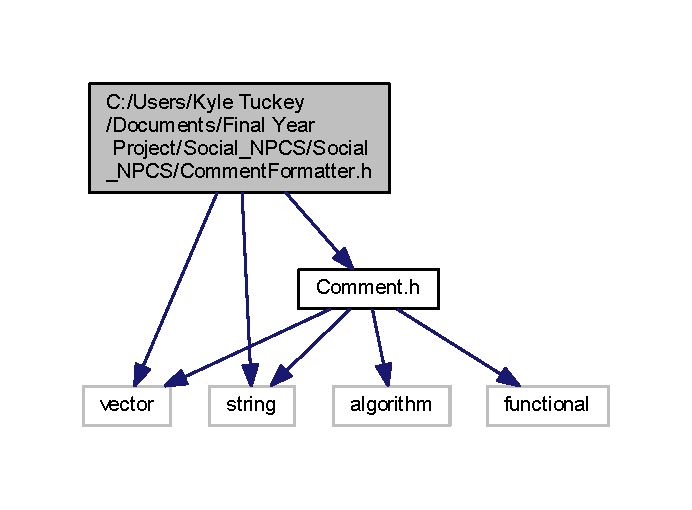
\includegraphics[width=332pt]{_comment_formatter_8h__incl}
\end{center}
\end{figure}
This graph shows which files directly or indirectly include this file\+:\nopagebreak
\begin{figure}[H]
\begin{center}
\leavevmode
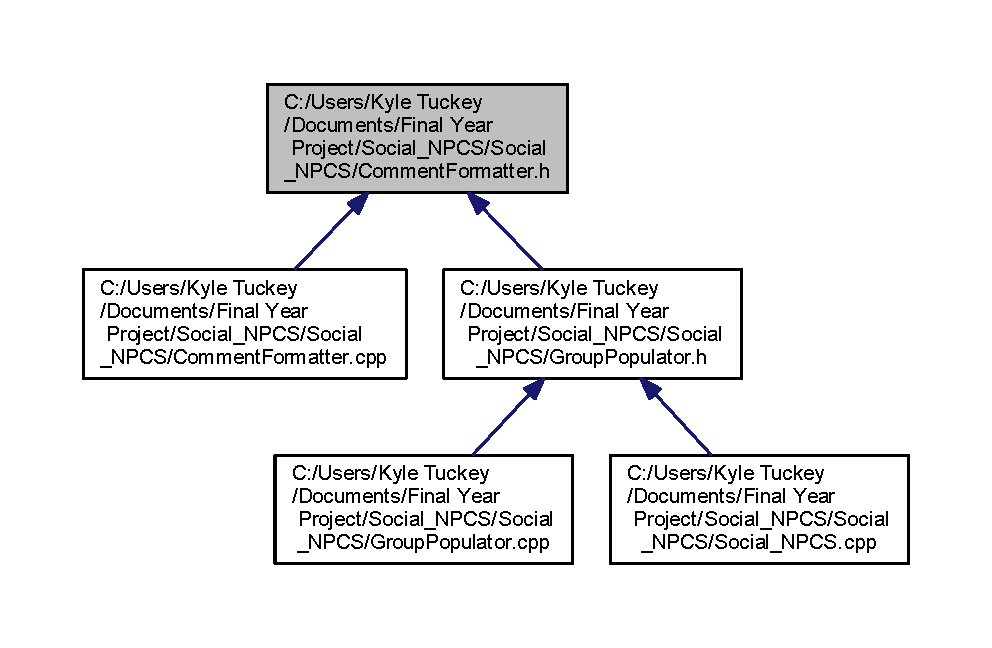
\includegraphics[width=350pt]{_comment_formatter_8h__dep__incl}
\end{center}
\end{figure}
\subsection*{Classes}
\begin{DoxyCompactItemize}
\item 
class \hyperlink{class_comment_formatter}{Comment\+Formatter}
\end{DoxyCompactItemize}

\hypertarget{comments_8py}{}\section{C\+:/\+Users/\+Kyle Tuckey/\+Documents/\+Final Year Project/\+Social\+\_\+\+N\+P\+C\+S/\+Social\+\_\+\+N\+P\+C\+S/comments.py File Reference}
\label{comments_8py}\index{C\+:/\+Users/\+Kyle Tuckey/\+Documents/\+Final Year Project/\+Social\+\_\+\+N\+P\+C\+S/\+Social\+\_\+\+N\+P\+C\+S/comments.\+py@{C\+:/\+Users/\+Kyle Tuckey/\+Documents/\+Final Year Project/\+Social\+\_\+\+N\+P\+C\+S/\+Social\+\_\+\+N\+P\+C\+S/comments.\+py}}
\subsection*{Classes}
\begin{DoxyCompactItemize}
\item 
class \hyperlink{classcomments_1_1_object}{comments.\+Object}
\end{DoxyCompactItemize}
\subsection*{Namespaces}
\begin{DoxyCompactItemize}
\item 
 \hyperlink{namespacecomments}{comments}
\end{DoxyCompactItemize}
\subsection*{Functions}
\begin{DoxyCompactItemize}
\item 
def \hyperlink{namespacecomments_a15146b34dd7b539d081e27278c3c322e}{comments.\+get\+Sentiment} (body)
\item 
def \hyperlink{namespacecomments_aadd79f53e655498635ea6597a88b219c}{comments.\+get\+Comments} ()
\end{DoxyCompactItemize}

\hypertarget{_group_8cpp}{}\section{C\+:/\+Users/\+Kyle Tuckey/\+Documents/\+Final Year Project/\+Social\+\_\+\+N\+P\+C\+S/\+Social\+\_\+\+N\+P\+C\+S/\+Group.cpp File Reference}
\label{_group_8cpp}\index{C\+:/\+Users/\+Kyle Tuckey/\+Documents/\+Final Year Project/\+Social\+\_\+\+N\+P\+C\+S/\+Social\+\_\+\+N\+P\+C\+S/\+Group.\+cpp@{C\+:/\+Users/\+Kyle Tuckey/\+Documents/\+Final Year Project/\+Social\+\_\+\+N\+P\+C\+S/\+Social\+\_\+\+N\+P\+C\+S/\+Group.\+cpp}}
{\ttfamily \#include \char`\"{}Group.\+h\char`\"{}}\newline
Include dependency graph for Group.\+cpp\+:\nopagebreak
\begin{figure}[H]
\begin{center}
\leavevmode
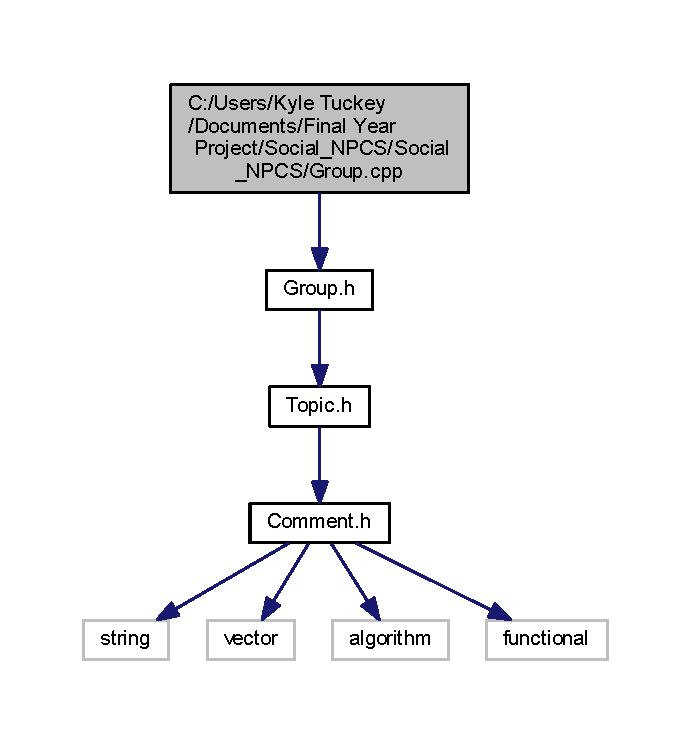
\includegraphics[width=332pt]{_group_8cpp__incl}
\end{center}
\end{figure}
\subsection*{Functions}
\begin{DoxyCompactItemize}
\item 
bool \hyperlink{_group_8cpp_a783c647cdb5e6d4a46a1f903f2af3ac8}{operator==} (const \hyperlink{class_group}{Group} \&t1, const \hyperlink{class_group}{Group} \&t2)
\end{DoxyCompactItemize}


\subsection{Function Documentation}
\mbox{\Hypertarget{_group_8cpp_a783c647cdb5e6d4a46a1f903f2af3ac8}\label{_group_8cpp_a783c647cdb5e6d4a46a1f903f2af3ac8}} 
\index{Group.\+cpp@{Group.\+cpp}!operator==@{operator==}}
\index{operator==@{operator==}!Group.\+cpp@{Group.\+cpp}}
\subsubsection{\texorpdfstring{operator==()}{operator==()}}
{\footnotesize\ttfamily bool operator== (\begin{DoxyParamCaption}\item[{const \hyperlink{class_group}{Group} \&}]{t1,  }\item[{const \hyperlink{class_group}{Group} \&}]{t2 }\end{DoxyParamCaption})}



Definition at line 31 of file Group.\+cpp.



References Group\+::id, and Group\+::topics.


\begin{DoxyCode}
32 \{
33     \textcolor{keywordflow}{return}  (t1.\hyperlink{class_group_ade135fec88f463adb44f780cb476e7d3}{id} == t2.\hyperlink{class_group_ade135fec88f463adb44f780cb476e7d3}{id}) && (t1.\hyperlink{class_group_a5927c259318d2058c9d1573110718bb5}{topics} == t2.\hyperlink{class_group_a5927c259318d2058c9d1573110718bb5}{topics});
34 \}
\end{DoxyCode}

\hypertarget{_group_8h}{}\section{C\+:/\+Users/\+Kyle Tuckey/\+Documents/\+Final Year Project/\+Social\+\_\+\+N\+P\+C\+S/\+Social\+\_\+\+N\+P\+C\+S/\+Group.h File Reference}
\label{_group_8h}\index{C\+:/\+Users/\+Kyle Tuckey/\+Documents/\+Final Year Project/\+Social\+\_\+\+N\+P\+C\+S/\+Social\+\_\+\+N\+P\+C\+S/\+Group.\+h@{C\+:/\+Users/\+Kyle Tuckey/\+Documents/\+Final Year Project/\+Social\+\_\+\+N\+P\+C\+S/\+Social\+\_\+\+N\+P\+C\+S/\+Group.\+h}}
{\ttfamily \#include \char`\"{}Topic.\+h\char`\"{}}\newline
Include dependency graph for Group.\+h\+:\nopagebreak
\begin{figure}[H]
\begin{center}
\leavevmode
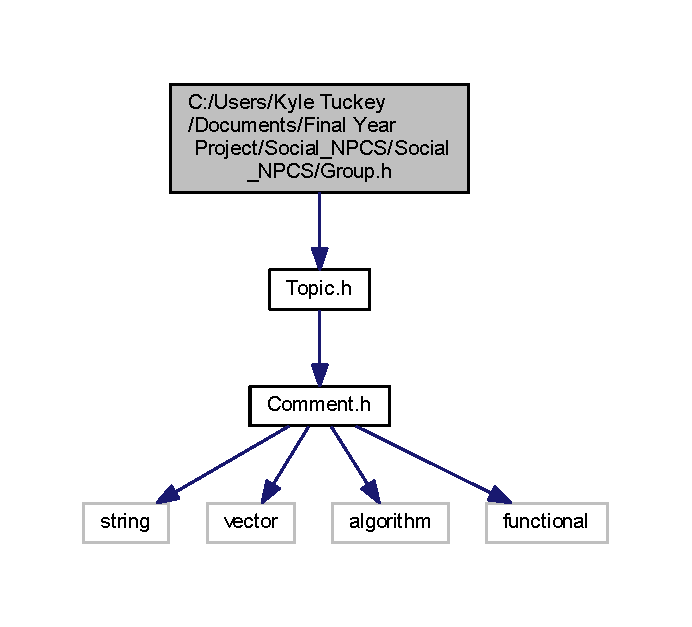
\includegraphics[width=332pt]{_group_8h__incl}
\end{center}
\end{figure}
This graph shows which files directly or indirectly include this file\+:\nopagebreak
\begin{figure}[H]
\begin{center}
\leavevmode
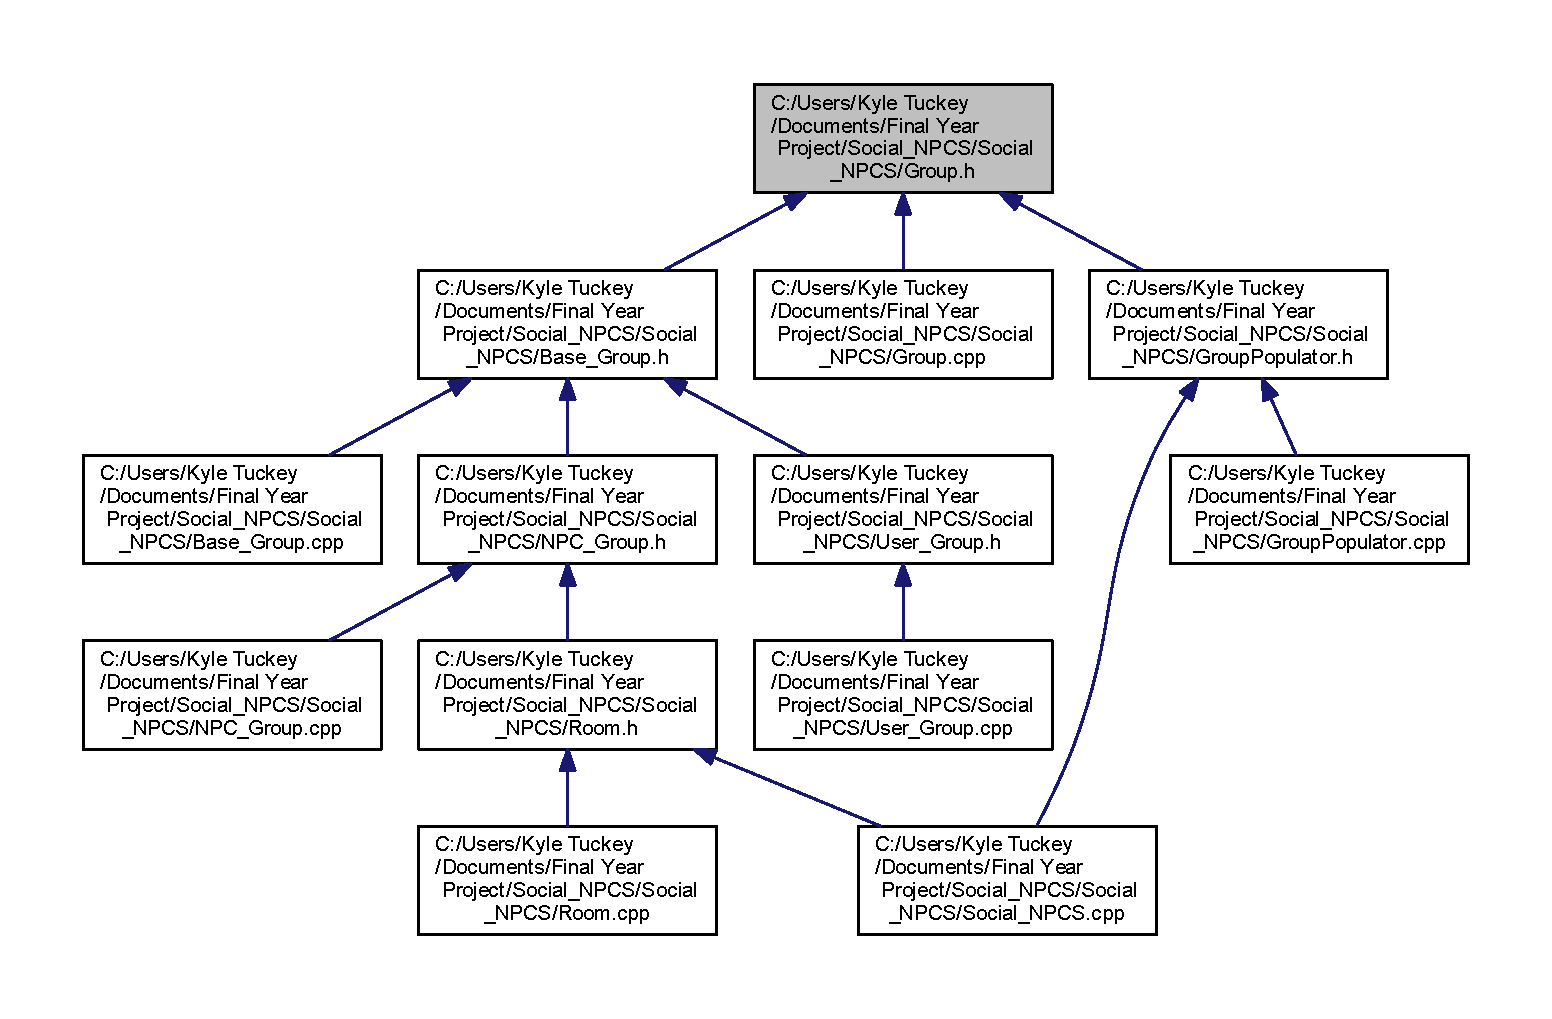
\includegraphics[width=350pt]{_group_8h__dep__incl}
\end{center}
\end{figure}
\subsection*{Classes}
\begin{DoxyCompactItemize}
\item 
class \hyperlink{class_group}{Group}
\end{DoxyCompactItemize}

\hypertarget{_group_populator_8cpp}{}\section{C\+:/\+Users/\+Kyle Tuckey/\+Documents/\+Final Year Project/\+Social\+\_\+\+N\+P\+C\+S/\+Social\+\_\+\+N\+P\+C\+S/\+Group\+Populator.cpp File Reference}
\label{_group_populator_8cpp}\index{C\+:/\+Users/\+Kyle Tuckey/\+Documents/\+Final Year Project/\+Social\+\_\+\+N\+P\+C\+S/\+Social\+\_\+\+N\+P\+C\+S/\+Group\+Populator.\+cpp@{C\+:/\+Users/\+Kyle Tuckey/\+Documents/\+Final Year Project/\+Social\+\_\+\+N\+P\+C\+S/\+Social\+\_\+\+N\+P\+C\+S/\+Group\+Populator.\+cpp}}
{\ttfamily \#include \char`\"{}Group\+Populator.\+h\char`\"{}}\newline
Include dependency graph for Group\+Populator.\+cpp\+:\nopagebreak
\begin{figure}[H]
\begin{center}
\leavevmode
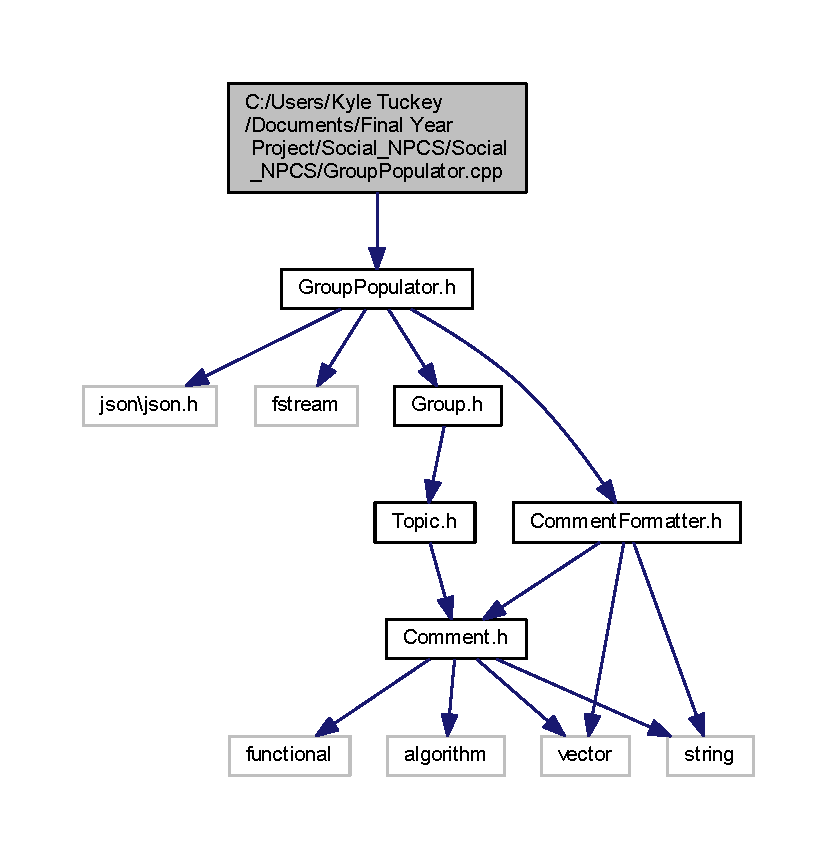
\includegraphics[width=350pt]{_group_populator_8cpp__incl}
\end{center}
\end{figure}

\hypertarget{_group_populator_8h}{}\section{C\+:/\+Users/\+Kyle Tuckey/\+Documents/\+Final Year Project/\+Social\+\_\+\+N\+P\+C\+S/\+Social\+\_\+\+N\+P\+C\+S/\+Group\+Populator.h File Reference}
\label{_group_populator_8h}\index{C\+:/\+Users/\+Kyle Tuckey/\+Documents/\+Final Year Project/\+Social\+\_\+\+N\+P\+C\+S/\+Social\+\_\+\+N\+P\+C\+S/\+Group\+Populator.\+h@{C\+:/\+Users/\+Kyle Tuckey/\+Documents/\+Final Year Project/\+Social\+\_\+\+N\+P\+C\+S/\+Social\+\_\+\+N\+P\+C\+S/\+Group\+Populator.\+h}}
{\ttfamily \#include $<$json\textbackslash{}json.\+h$>$}\newline
{\ttfamily \#include $<$fstream$>$}\newline
{\ttfamily \#include \char`\"{}Group.\+h\char`\"{}}\newline
{\ttfamily \#include \char`\"{}Comment\+Formatter.\+h\char`\"{}}\newline
Include dependency graph for Group\+Populator.\+h\+:\nopagebreak
\begin{figure}[H]
\begin{center}
\leavevmode
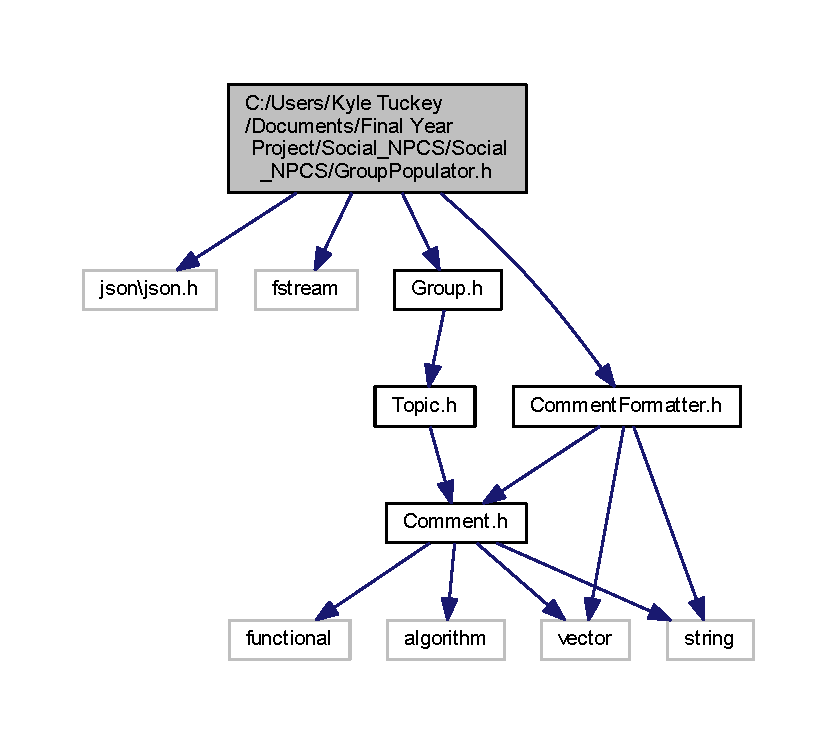
\includegraphics[width=350pt]{_group_populator_8h__incl}
\end{center}
\end{figure}
This graph shows which files directly or indirectly include this file\+:\nopagebreak
\begin{figure}[H]
\begin{center}
\leavevmode
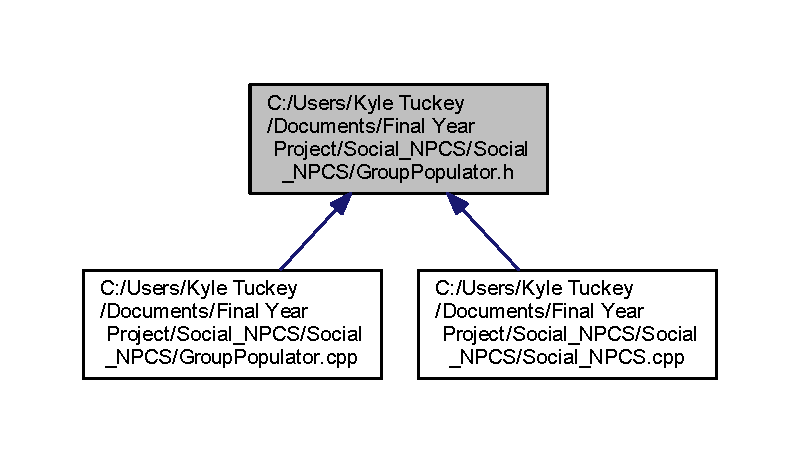
\includegraphics[width=350pt]{_group_populator_8h__dep__incl}
\end{center}
\end{figure}
\subsection*{Classes}
\begin{DoxyCompactItemize}
\item 
class \hyperlink{class_group_populator}{Group\+Populator}
\end{DoxyCompactItemize}

\hypertarget{_j_s_o_n_reader_8cpp}{}\section{C\+:/\+Users/\+Kyle Tuckey/\+Documents/\+Final Year Project/\+Social\+\_\+\+N\+P\+C\+S/\+Social\+\_\+\+N\+P\+C\+S/\+J\+S\+O\+N\+Reader.cpp File Reference}
\label{_j_s_o_n_reader_8cpp}\index{C\+:/\+Users/\+Kyle Tuckey/\+Documents/\+Final Year Project/\+Social\+\_\+\+N\+P\+C\+S/\+Social\+\_\+\+N\+P\+C\+S/\+J\+S\+O\+N\+Reader.\+cpp@{C\+:/\+Users/\+Kyle Tuckey/\+Documents/\+Final Year Project/\+Social\+\_\+\+N\+P\+C\+S/\+Social\+\_\+\+N\+P\+C\+S/\+J\+S\+O\+N\+Reader.\+cpp}}
{\ttfamily \#include \char`\"{}J\+S\+O\+N\+Reader.\+h\char`\"{}}\newline
Include dependency graph for J\+S\+O\+N\+Reader.\+cpp\+:\nopagebreak
\begin{figure}[H]
\begin{center}
\leavevmode
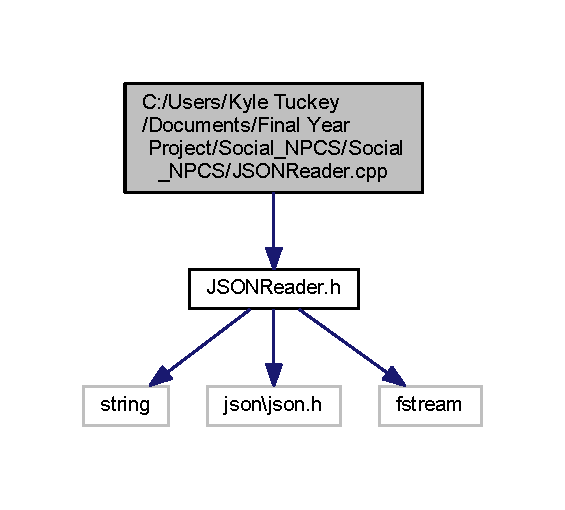
\includegraphics[width=271pt]{_j_s_o_n_reader_8cpp__incl}
\end{center}
\end{figure}

\hypertarget{_j_s_o_n_reader_8h}{}\section{C\+:/\+Users/\+Kyle Tuckey/\+Documents/\+Final Year Project/\+Social\+\_\+\+N\+P\+C\+S/\+Social\+\_\+\+N\+P\+C\+S/\+J\+S\+O\+N\+Reader.h File Reference}
\label{_j_s_o_n_reader_8h}\index{C\+:/\+Users/\+Kyle Tuckey/\+Documents/\+Final Year Project/\+Social\+\_\+\+N\+P\+C\+S/\+Social\+\_\+\+N\+P\+C\+S/\+J\+S\+O\+N\+Reader.\+h@{C\+:/\+Users/\+Kyle Tuckey/\+Documents/\+Final Year Project/\+Social\+\_\+\+N\+P\+C\+S/\+Social\+\_\+\+N\+P\+C\+S/\+J\+S\+O\+N\+Reader.\+h}}
{\ttfamily \#include $<$string$>$}\newline
{\ttfamily \#include $<$json\textbackslash{}json.\+h$>$}\newline
{\ttfamily \#include $<$fstream$>$}\newline
Include dependency graph for J\+S\+O\+N\+Reader.\+h\+:\nopagebreak
\begin{figure}[H]
\begin{center}
\leavevmode
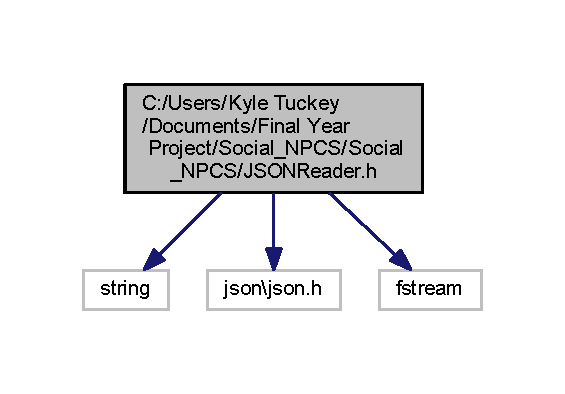
\includegraphics[width=271pt]{_j_s_o_n_reader_8h__incl}
\end{center}
\end{figure}
This graph shows which files directly or indirectly include this file\+:\nopagebreak
\begin{figure}[H]
\begin{center}
\leavevmode
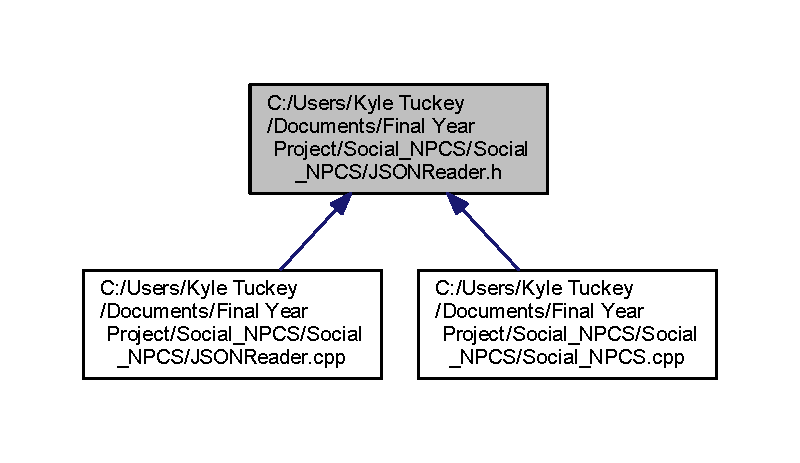
\includegraphics[width=350pt]{_j_s_o_n_reader_8h__dep__incl}
\end{center}
\end{figure}
\subsection*{Classes}
\begin{DoxyCompactItemize}
\item 
class \hyperlink{class_j_s_o_n_reader}{J\+S\+O\+N\+Reader}
\end{DoxyCompactItemize}

\hypertarget{_node_8cpp}{}\section{C\+:/\+Users/\+Kyle Tuckey/\+Documents/\+Final Year Project/\+Social\+\_\+\+N\+P\+C\+S/\+Social\+\_\+\+N\+P\+C\+S/\+Node.cpp File Reference}
\label{_node_8cpp}\index{C\+:/\+Users/\+Kyle Tuckey/\+Documents/\+Final Year Project/\+Social\+\_\+\+N\+P\+C\+S/\+Social\+\_\+\+N\+P\+C\+S/\+Node.\+cpp@{C\+:/\+Users/\+Kyle Tuckey/\+Documents/\+Final Year Project/\+Social\+\_\+\+N\+P\+C\+S/\+Social\+\_\+\+N\+P\+C\+S/\+Node.\+cpp}}
{\ttfamily \#include \char`\"{}Node.\+h\char`\"{}}\newline
Include dependency graph for Node.\+cpp\+:\nopagebreak
\begin{figure}[H]
\begin{center}
\leavevmode
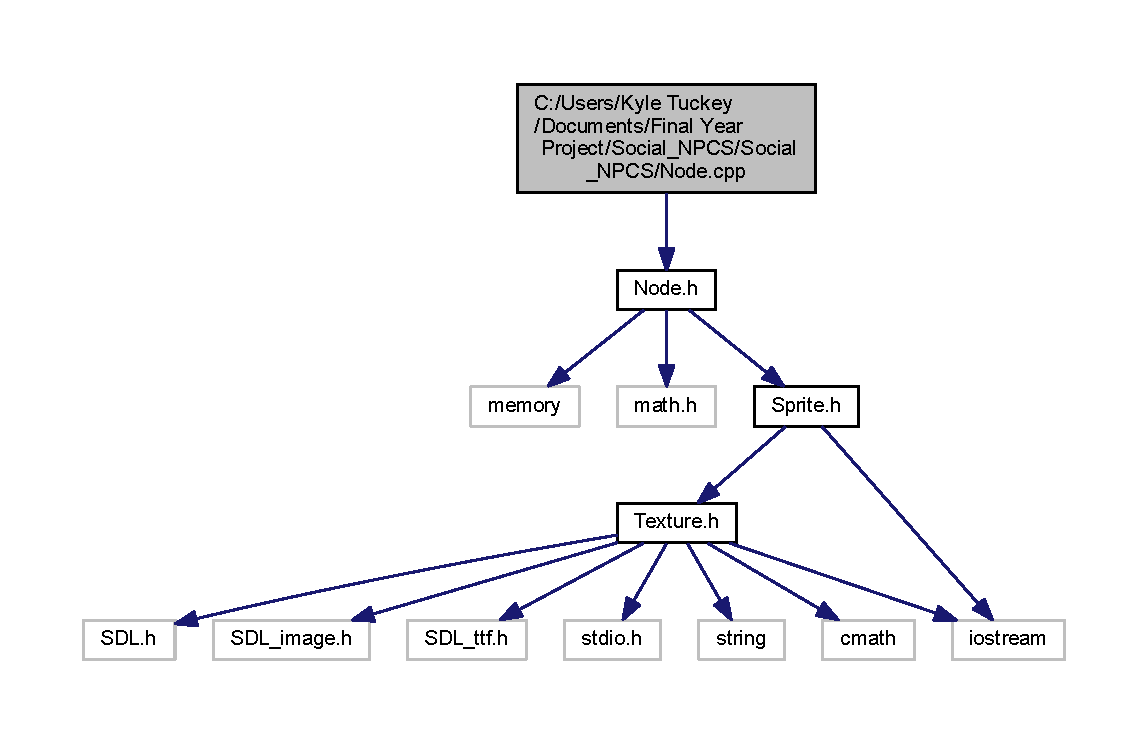
\includegraphics[width=350pt]{_node_8cpp__incl}
\end{center}
\end{figure}

\hypertarget{_node_8h}{}\section{C\+:/\+Users/\+Kyle Tuckey/\+Documents/\+Final Year Project/\+Social\+\_\+\+N\+P\+C\+S/\+Social\+\_\+\+N\+P\+C\+S/\+Node.h File Reference}
\label{_node_8h}\index{C\+:/\+Users/\+Kyle Tuckey/\+Documents/\+Final Year Project/\+Social\+\_\+\+N\+P\+C\+S/\+Social\+\_\+\+N\+P\+C\+S/\+Node.\+h@{C\+:/\+Users/\+Kyle Tuckey/\+Documents/\+Final Year Project/\+Social\+\_\+\+N\+P\+C\+S/\+Social\+\_\+\+N\+P\+C\+S/\+Node.\+h}}
{\ttfamily \#include $<$memory$>$}\newline
{\ttfamily \#include $<$math.\+h$>$}\newline
{\ttfamily \#include \char`\"{}Sprite.\+h\char`\"{}}\newline
Include dependency graph for Node.\+h\+:\nopagebreak
\begin{figure}[H]
\begin{center}
\leavevmode
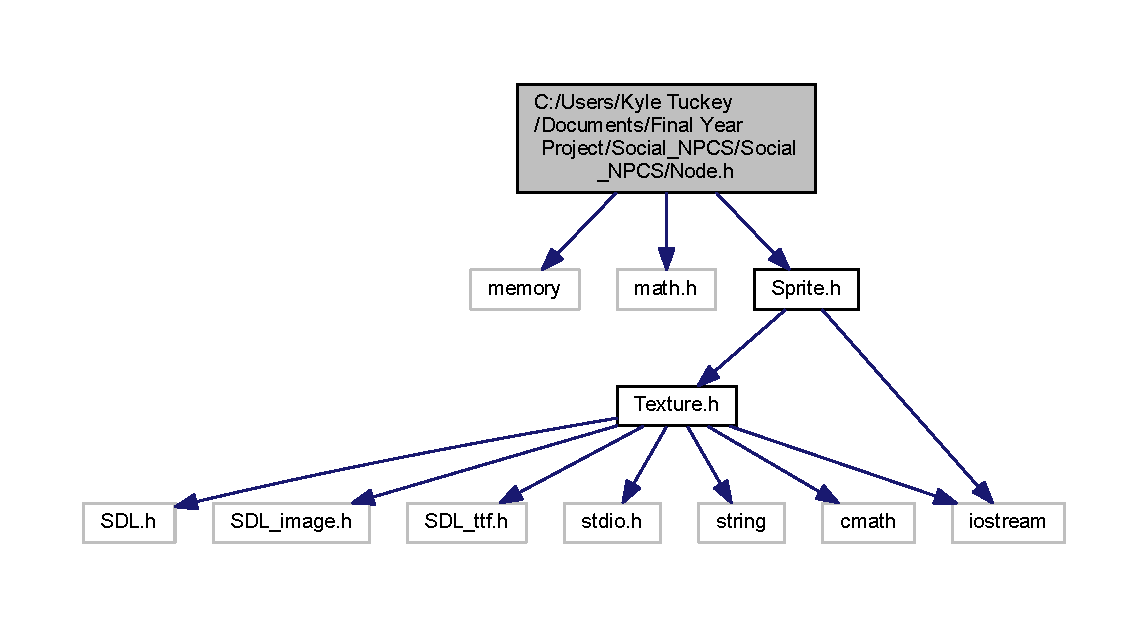
\includegraphics[width=350pt]{_node_8h__incl}
\end{center}
\end{figure}
This graph shows which files directly or indirectly include this file\+:\nopagebreak
\begin{figure}[H]
\begin{center}
\leavevmode
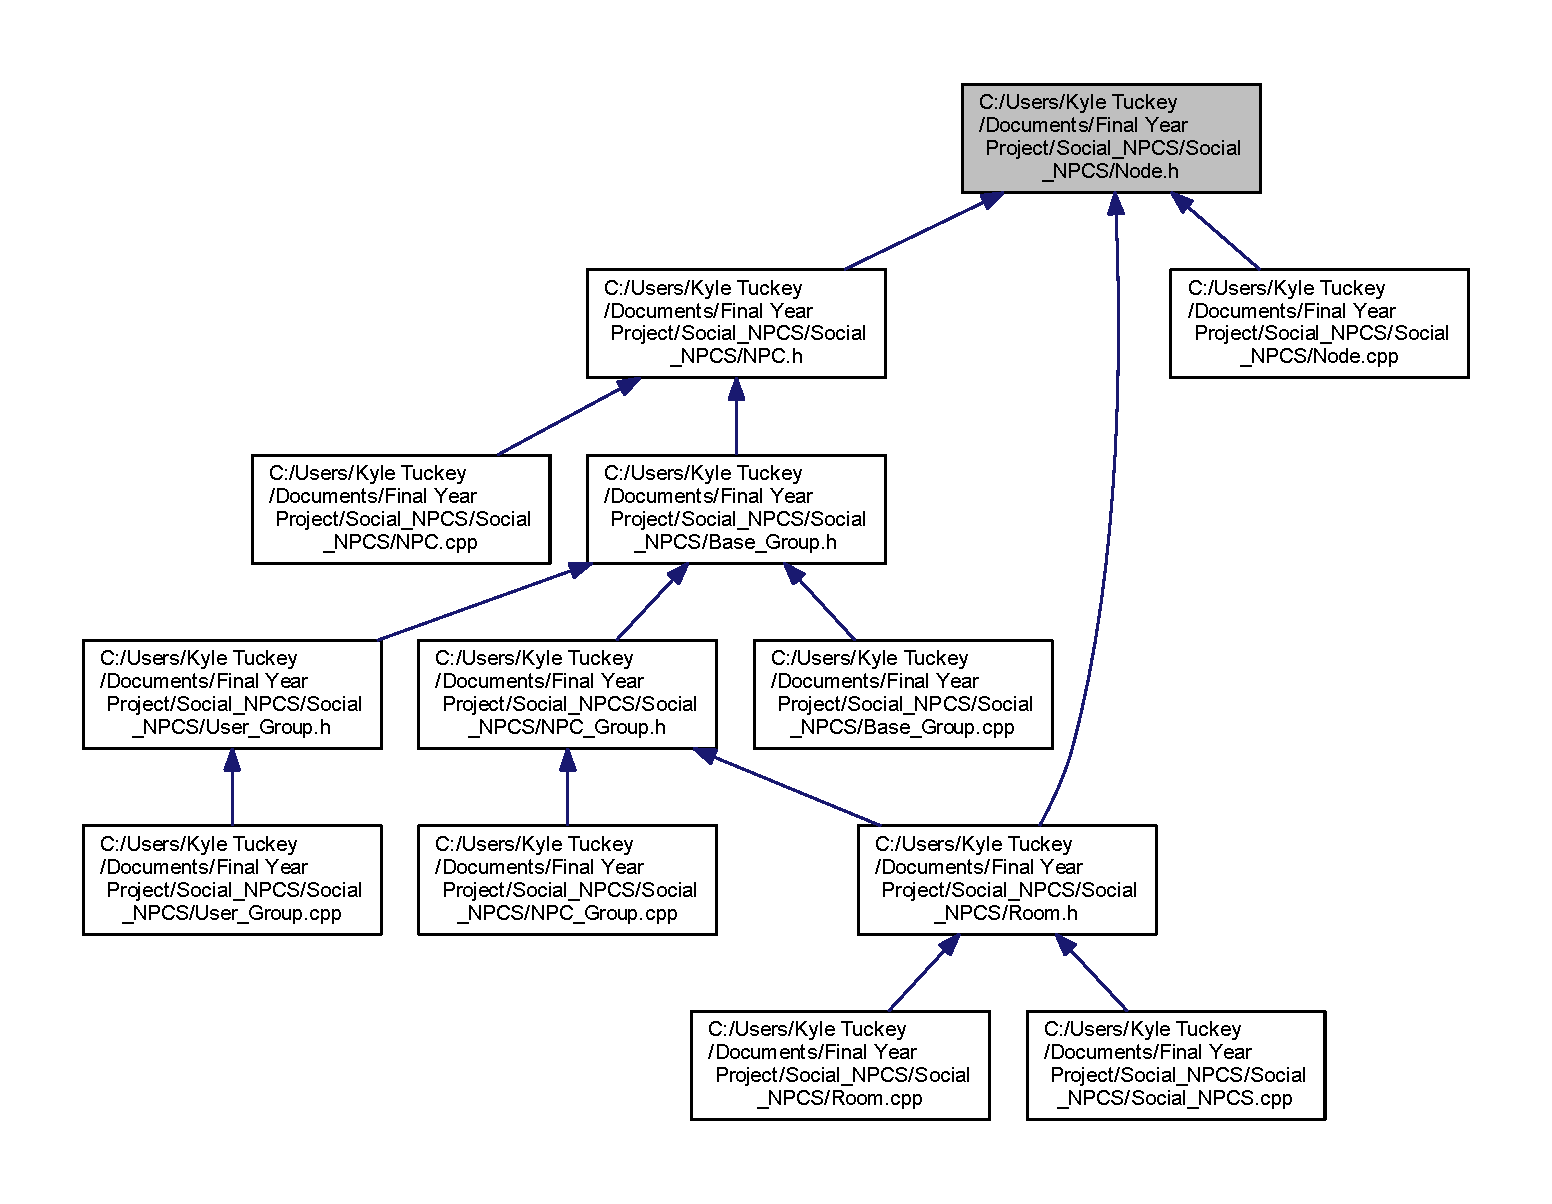
\includegraphics[width=350pt]{_node_8h__dep__incl}
\end{center}
\end{figure}
\subsection*{Classes}
\begin{DoxyCompactItemize}
\item 
class \hyperlink{class_node}{Node}
\end{DoxyCompactItemize}
\subsection*{Macros}
\begin{DoxyCompactItemize}
\item 
\#define \hyperlink{_node_8h_ad09d43a79456fb527b624510744dae59}{W\+O\+R\+L\+D\+\_\+\+S\+I\+ZE}~= 800;
\end{DoxyCompactItemize}


\subsection{Macro Definition Documentation}
\mbox{\Hypertarget{_node_8h_ad09d43a79456fb527b624510744dae59}\label{_node_8h_ad09d43a79456fb527b624510744dae59}} 
\index{Node.\+h@{Node.\+h}!W\+O\+R\+L\+D\+\_\+\+S\+I\+ZE@{W\+O\+R\+L\+D\+\_\+\+S\+I\+ZE}}
\index{W\+O\+R\+L\+D\+\_\+\+S\+I\+ZE@{W\+O\+R\+L\+D\+\_\+\+S\+I\+ZE}!Node.\+h@{Node.\+h}}
\subsubsection{\texorpdfstring{W\+O\+R\+L\+D\+\_\+\+S\+I\+ZE}{WORLD\_SIZE}}
{\footnotesize\ttfamily \#define W\+O\+R\+L\+D\+\_\+\+S\+I\+ZE~= 800;}



Definition at line 7 of file Node.\+h.


\hypertarget{_n_p_c_8cpp}{}\section{C\+:/\+Users/\+Kyle Tuckey/\+Documents/\+Final Year Project/\+Social\+\_\+\+N\+P\+C\+S/\+Social\+\_\+\+N\+P\+C\+S/\+N\+PC.cpp File Reference}
\label{_n_p_c_8cpp}\index{C\+:/\+Users/\+Kyle Tuckey/\+Documents/\+Final Year Project/\+Social\+\_\+\+N\+P\+C\+S/\+Social\+\_\+\+N\+P\+C\+S/\+N\+P\+C.\+cpp@{C\+:/\+Users/\+Kyle Tuckey/\+Documents/\+Final Year Project/\+Social\+\_\+\+N\+P\+C\+S/\+Social\+\_\+\+N\+P\+C\+S/\+N\+P\+C.\+cpp}}
{\ttfamily \#include \char`\"{}N\+P\+C.\+h\char`\"{}}\newline
Include dependency graph for N\+P\+C.\+cpp\+:\nopagebreak
\begin{figure}[H]
\begin{center}
\leavevmode
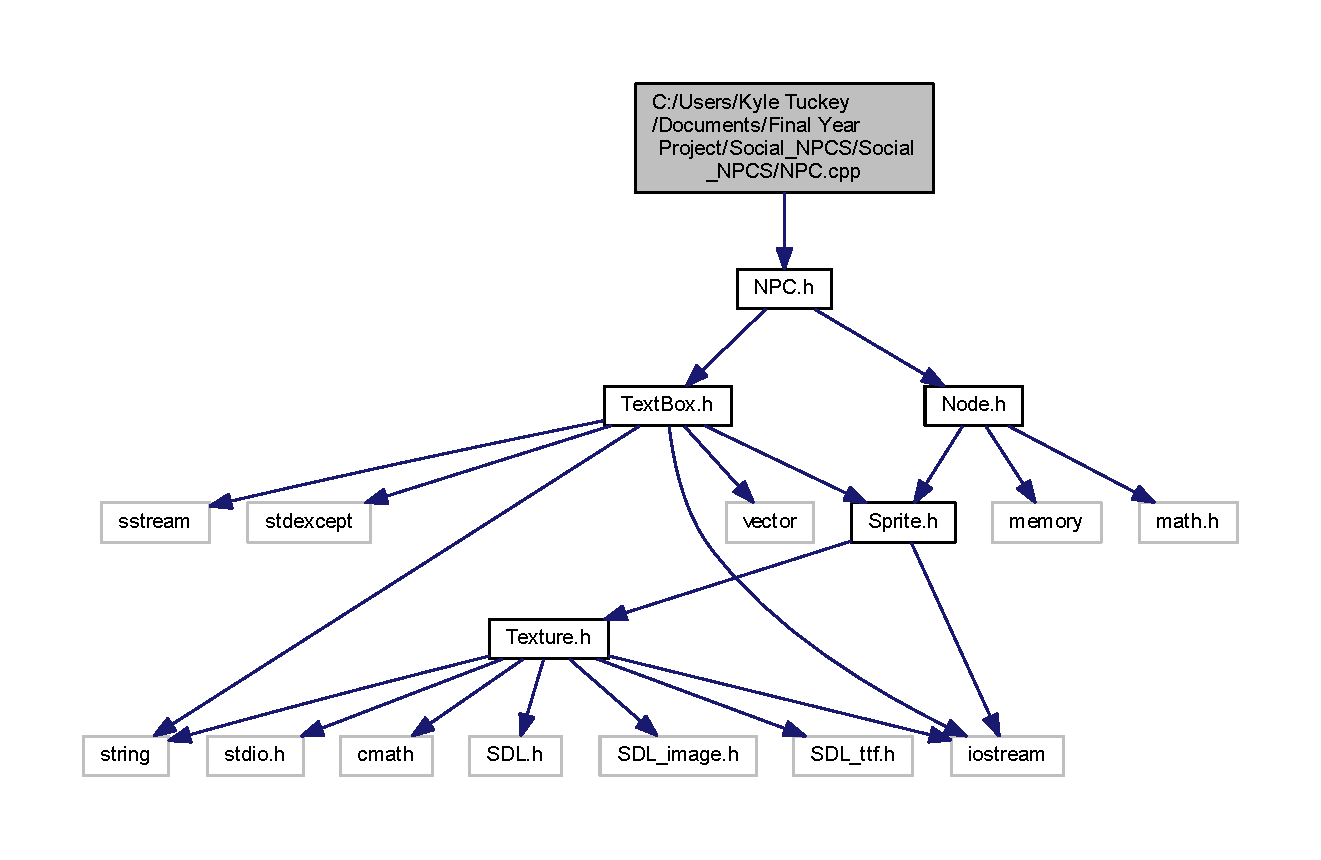
\includegraphics[width=350pt]{_n_p_c_8cpp__incl}
\end{center}
\end{figure}
\subsection*{Functions}
\begin{DoxyCompactItemize}
\item 
bool \hyperlink{_n_p_c_8cpp_a3e1f9defd10ab4be568a190fbcd0ac07}{operator==} (const \hyperlink{class_n_p_c}{N\+PC} \&c1, const \hyperlink{class_n_p_c}{N\+PC} \&c2)
\end{DoxyCompactItemize}


\subsection{Function Documentation}
\mbox{\Hypertarget{_n_p_c_8cpp_a3e1f9defd10ab4be568a190fbcd0ac07}\label{_n_p_c_8cpp_a3e1f9defd10ab4be568a190fbcd0ac07}} 
\index{N\+P\+C.\+cpp@{N\+P\+C.\+cpp}!operator==@{operator==}}
\index{operator==@{operator==}!N\+P\+C.\+cpp@{N\+P\+C.\+cpp}}
\subsubsection{\texorpdfstring{operator==()}{operator==()}}
{\footnotesize\ttfamily bool operator== (\begin{DoxyParamCaption}\item[{const \hyperlink{class_n_p_c}{N\+PC} \&}]{c1,  }\item[{const \hyperlink{class_n_p_c}{N\+PC} \&}]{c2 }\end{DoxyParamCaption})}



Definition at line 263 of file N\+P\+C.\+cpp.



References N\+P\+C\+::id.


\begin{DoxyCode}
264 \{
265     \textcolor{keywordflow}{return} (c1.\hyperlink{class_n_p_c_a1b705223f885df652f2faffc4735d03c}{id} == c2.\hyperlink{class_n_p_c_a1b705223f885df652f2faffc4735d03c}{id});
266 \}
\end{DoxyCode}

\hypertarget{_n_p_c_8h}{}\section{C\+:/\+Users/\+Kyle Tuckey/\+Documents/\+Final Year Project/\+Social\+\_\+\+N\+P\+C\+S/\+Social\+\_\+\+N\+P\+C\+S/\+N\+PC.h File Reference}
\label{_n_p_c_8h}\index{C\+:/\+Users/\+Kyle Tuckey/\+Documents/\+Final Year Project/\+Social\+\_\+\+N\+P\+C\+S/\+Social\+\_\+\+N\+P\+C\+S/\+N\+P\+C.\+h@{C\+:/\+Users/\+Kyle Tuckey/\+Documents/\+Final Year Project/\+Social\+\_\+\+N\+P\+C\+S/\+Social\+\_\+\+N\+P\+C\+S/\+N\+P\+C.\+h}}
{\ttfamily \#include \char`\"{}Text\+Box.\+h\char`\"{}}\newline
{\ttfamily \#include \char`\"{}Node.\+h\char`\"{}}\newline
Include dependency graph for N\+P\+C.\+h\+:\nopagebreak
\begin{figure}[H]
\begin{center}
\leavevmode
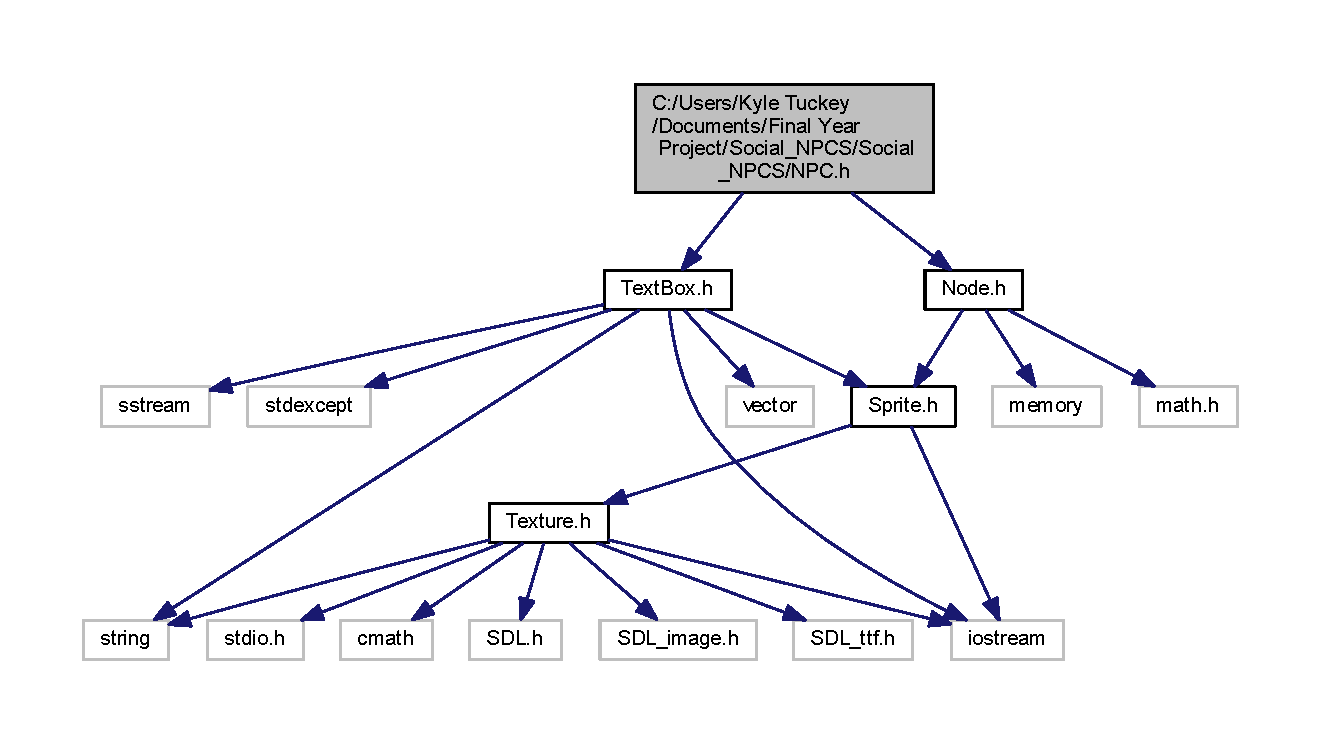
\includegraphics[width=350pt]{_n_p_c_8h__incl}
\end{center}
\end{figure}
This graph shows which files directly or indirectly include this file\+:\nopagebreak
\begin{figure}[H]
\begin{center}
\leavevmode
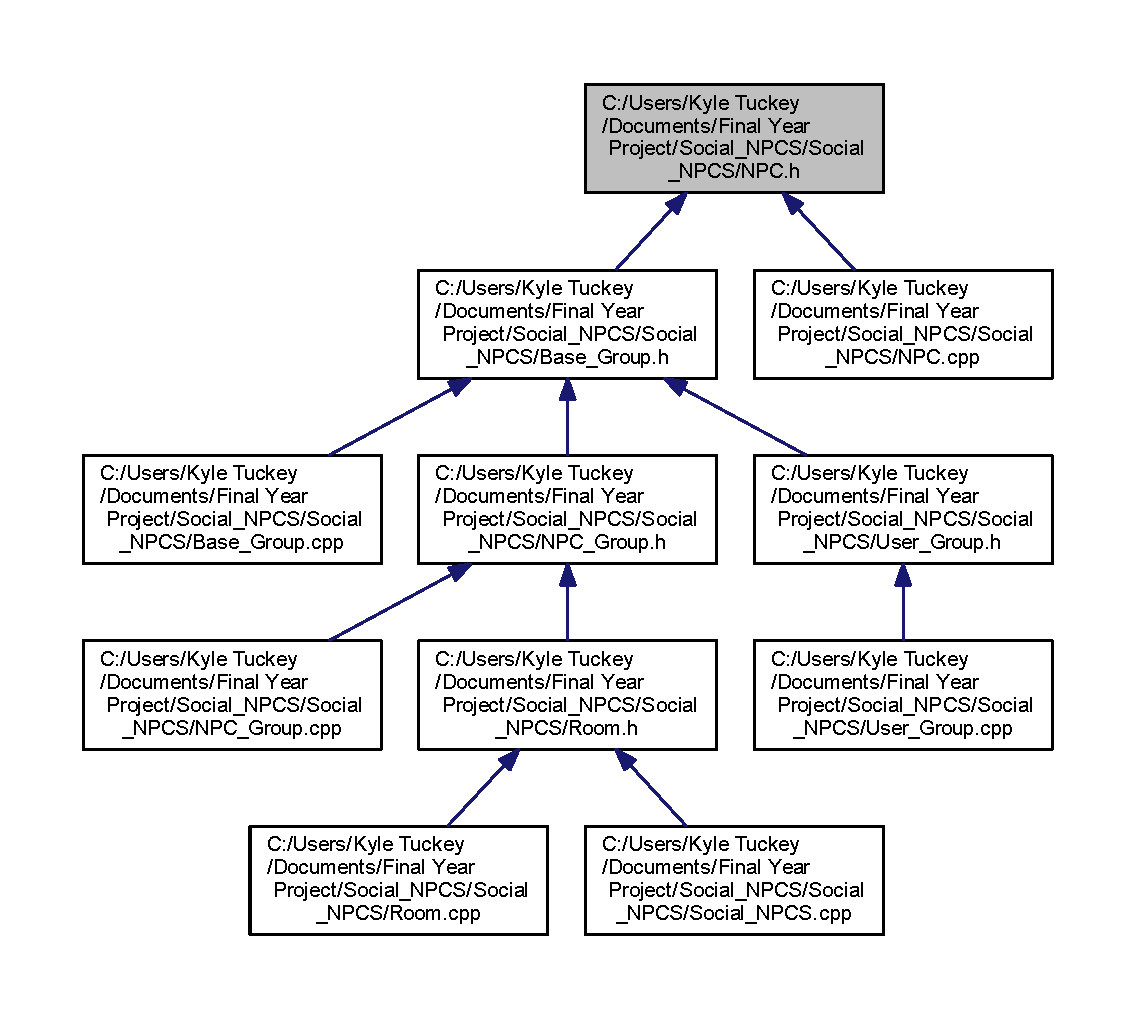
\includegraphics[width=350pt]{_n_p_c_8h__dep__incl}
\end{center}
\end{figure}
\subsection*{Classes}
\begin{DoxyCompactItemize}
\item 
class \hyperlink{class_n_p_c}{N\+PC}
\end{DoxyCompactItemize}

\hypertarget{_n_p_c___group_8cpp}{}\section{C\+:/\+Users/\+Kyle Tuckey/\+Documents/\+Final Year Project/\+Social\+\_\+\+N\+P\+C\+S/\+Social\+\_\+\+N\+P\+C\+S/\+N\+P\+C\+\_\+\+Group.cpp File Reference}
\label{_n_p_c___group_8cpp}\index{C\+:/\+Users/\+Kyle Tuckey/\+Documents/\+Final Year Project/\+Social\+\_\+\+N\+P\+C\+S/\+Social\+\_\+\+N\+P\+C\+S/\+N\+P\+C\+\_\+\+Group.\+cpp@{C\+:/\+Users/\+Kyle Tuckey/\+Documents/\+Final Year Project/\+Social\+\_\+\+N\+P\+C\+S/\+Social\+\_\+\+N\+P\+C\+S/\+N\+P\+C\+\_\+\+Group.\+cpp}}
{\ttfamily \#include \char`\"{}N\+P\+C\+\_\+\+Group.\+h\char`\"{}}\newline
Include dependency graph for N\+P\+C\+\_\+\+Group.\+cpp\+:\nopagebreak
\begin{figure}[H]
\begin{center}
\leavevmode
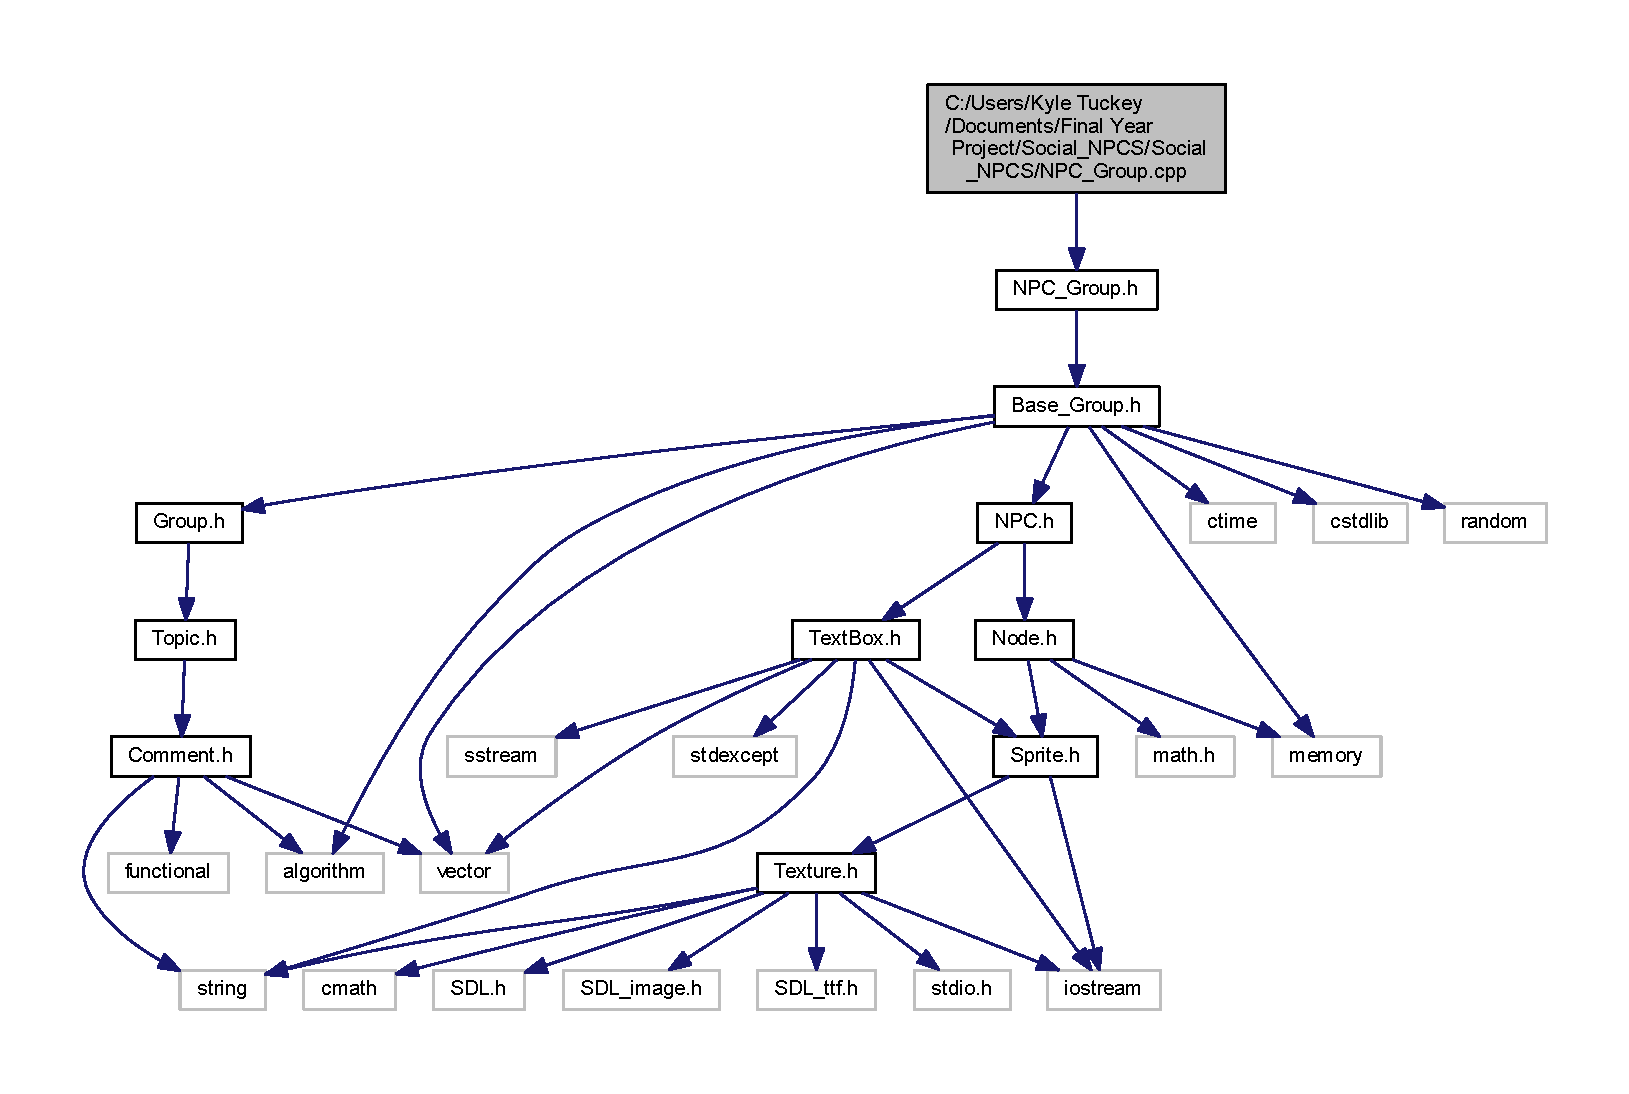
\includegraphics[width=350pt]{_n_p_c___group_8cpp__incl}
\end{center}
\end{figure}

\hypertarget{_n_p_c___group_8h}{}\section{C\+:/\+Users/\+Kyle Tuckey/\+Documents/\+Final Year Project/\+Social\+\_\+\+N\+P\+C\+S/\+Social\+\_\+\+N\+P\+C\+S/\+N\+P\+C\+\_\+\+Group.h File Reference}
\label{_n_p_c___group_8h}\index{C\+:/\+Users/\+Kyle Tuckey/\+Documents/\+Final Year Project/\+Social\+\_\+\+N\+P\+C\+S/\+Social\+\_\+\+N\+P\+C\+S/\+N\+P\+C\+\_\+\+Group.\+h@{C\+:/\+Users/\+Kyle Tuckey/\+Documents/\+Final Year Project/\+Social\+\_\+\+N\+P\+C\+S/\+Social\+\_\+\+N\+P\+C\+S/\+N\+P\+C\+\_\+\+Group.\+h}}
{\ttfamily \#include \char`\"{}Base\+\_\+\+Group.\+h\char`\"{}}\newline
Include dependency graph for N\+P\+C\+\_\+\+Group.\+h\+:\nopagebreak
\begin{figure}[H]
\begin{center}
\leavevmode
\includegraphics[width=350pt]{_n_p_c___group_8h__incl}
\end{center}
\end{figure}
This graph shows which files directly or indirectly include this file\+:\nopagebreak
\begin{figure}[H]
\begin{center}
\leavevmode
\includegraphics[width=350pt]{_n_p_c___group_8h__dep__incl}
\end{center}
\end{figure}
\subsection*{Classes}
\begin{DoxyCompactItemize}
\item 
class \hyperlink{class_n_p_c___group}{N\+P\+C\+\_\+\+Group}
\end{DoxyCompactItemize}

\hypertarget{_python_handler_8cpp}{}\section{C\+:/\+Users/\+Kyle Tuckey/\+Documents/\+Final Year Project/\+Social\+\_\+\+N\+P\+C\+S/\+Social\+\_\+\+N\+P\+C\+S/\+Python\+Handler.cpp File Reference}
\label{_python_handler_8cpp}\index{C\+:/\+Users/\+Kyle Tuckey/\+Documents/\+Final Year Project/\+Social\+\_\+\+N\+P\+C\+S/\+Social\+\_\+\+N\+P\+C\+S/\+Python\+Handler.\+cpp@{C\+:/\+Users/\+Kyle Tuckey/\+Documents/\+Final Year Project/\+Social\+\_\+\+N\+P\+C\+S/\+Social\+\_\+\+N\+P\+C\+S/\+Python\+Handler.\+cpp}}
{\ttfamily \#include \char`\"{}Python\+Handler.\+h\char`\"{}}\newline
Include dependency graph for Python\+Handler.\+cpp\+:\nopagebreak
\begin{figure}[H]
\begin{center}
\leavevmode
\includegraphics[width=223pt]{_python_handler_8cpp__incl}
\end{center}
\end{figure}

\hypertarget{_python_handler_8h}{}\section{C\+:/\+Users/\+Kyle Tuckey/\+Documents/\+Final Year Project/\+Social\+\_\+\+N\+P\+C\+S/\+Social\+\_\+\+N\+P\+C\+S/\+Python\+Handler.h File Reference}
\label{_python_handler_8h}\index{C\+:/\+Users/\+Kyle Tuckey/\+Documents/\+Final Year Project/\+Social\+\_\+\+N\+P\+C\+S/\+Social\+\_\+\+N\+P\+C\+S/\+Python\+Handler.\+h@{C\+:/\+Users/\+Kyle Tuckey/\+Documents/\+Final Year Project/\+Social\+\_\+\+N\+P\+C\+S/\+Social\+\_\+\+N\+P\+C\+S/\+Python\+Handler.\+h}}
{\ttfamily \#include $<$Python.\+h$>$}\newline
{\ttfamily \#include $<$string$>$}\newline
Include dependency graph for Python\+Handler.\+h\+:\nopagebreak
\begin{figure}[H]
\begin{center}
\leavevmode
\includegraphics[width=223pt]{_python_handler_8h__incl}
\end{center}
\end{figure}
This graph shows which files directly or indirectly include this file\+:\nopagebreak
\begin{figure}[H]
\begin{center}
\leavevmode
\includegraphics[width=350pt]{_python_handler_8h__dep__incl}
\end{center}
\end{figure}
\subsection*{Classes}
\begin{DoxyCompactItemize}
\item 
class \hyperlink{class_python_handler}{Python\+Handler}
\end{DoxyCompactItemize}

\hypertarget{_resource_data_8cpp}{}\section{C\+:/\+Users/\+Kyle Tuckey/\+Documents/\+Final Year Project/\+Social\+\_\+\+N\+P\+C\+S/\+Social\+\_\+\+N\+P\+C\+S/\+Resource\+Data.cpp File Reference}
\label{_resource_data_8cpp}\index{C\+:/\+Users/\+Kyle Tuckey/\+Documents/\+Final Year Project/\+Social\+\_\+\+N\+P\+C\+S/\+Social\+\_\+\+N\+P\+C\+S/\+Resource\+Data.\+cpp@{C\+:/\+Users/\+Kyle Tuckey/\+Documents/\+Final Year Project/\+Social\+\_\+\+N\+P\+C\+S/\+Social\+\_\+\+N\+P\+C\+S/\+Resource\+Data.\+cpp}}
{\ttfamily \#include \char`\"{}Resource\+Data.\+h\char`\"{}}\newline
Include dependency graph for Resource\+Data.\+cpp\+:\nopagebreak
\begin{figure}[H]
\begin{center}
\leavevmode
\includegraphics[width=271pt]{_resource_data_8cpp__incl}
\end{center}
\end{figure}

\hypertarget{_resource_data_8h}{}\section{C\+:/\+Users/\+Kyle Tuckey/\+Documents/\+Final Year Project/\+Social\+\_\+\+N\+P\+C\+S/\+Social\+\_\+\+N\+P\+C\+S/\+Resource\+Data.h File Reference}
\label{_resource_data_8h}\index{C\+:/\+Users/\+Kyle Tuckey/\+Documents/\+Final Year Project/\+Social\+\_\+\+N\+P\+C\+S/\+Social\+\_\+\+N\+P\+C\+S/\+Resource\+Data.\+h@{C\+:/\+Users/\+Kyle Tuckey/\+Documents/\+Final Year Project/\+Social\+\_\+\+N\+P\+C\+S/\+Social\+\_\+\+N\+P\+C\+S/\+Resource\+Data.\+h}}
{\ttfamily \#include $<$json/json.\+h$>$}\newline
{\ttfamily \#include $<$string$>$}\newline
{\ttfamily \#include $<$fstream$>$}\newline
Include dependency graph for Resource\+Data.\+h\+:\nopagebreak
\begin{figure}[H]
\begin{center}
\leavevmode
\includegraphics[width=271pt]{_resource_data_8h__incl}
\end{center}
\end{figure}
This graph shows which files directly or indirectly include this file\+:\nopagebreak
\begin{figure}[H]
\begin{center}
\leavevmode
\includegraphics[width=350pt]{_resource_data_8h__dep__incl}
\end{center}
\end{figure}
\subsection*{Classes}
\begin{DoxyCompactItemize}
\item 
class \hyperlink{class_resource_data}{Resource\+Data}
\end{DoxyCompactItemize}

\hypertarget{_room_8cpp}{}\section{C\+:/\+Users/\+Kyle Tuckey/\+Documents/\+Final Year Project/\+Social\+\_\+\+N\+P\+C\+S/\+Social\+\_\+\+N\+P\+C\+S/\+Room.cpp File Reference}
\label{_room_8cpp}\index{C\+:/\+Users/\+Kyle Tuckey/\+Documents/\+Final Year Project/\+Social\+\_\+\+N\+P\+C\+S/\+Social\+\_\+\+N\+P\+C\+S/\+Room.\+cpp@{C\+:/\+Users/\+Kyle Tuckey/\+Documents/\+Final Year Project/\+Social\+\_\+\+N\+P\+C\+S/\+Social\+\_\+\+N\+P\+C\+S/\+Room.\+cpp}}
{\ttfamily \#include \char`\"{}Room.\+h\char`\"{}}\newline
Include dependency graph for Room.\+cpp\+:\nopagebreak
\begin{figure}[H]
\begin{center}
\leavevmode
\includegraphics[width=350pt]{_room_8cpp__incl}
\end{center}
\end{figure}

\hypertarget{_room_8h}{}\section{C\+:/\+Users/\+Kyle Tuckey/\+Documents/\+Final Year Project/\+Social\+\_\+\+N\+P\+C\+S/\+Social\+\_\+\+N\+P\+C\+S/\+Room.h File Reference}
\label{_room_8h}\index{C\+:/\+Users/\+Kyle Tuckey/\+Documents/\+Final Year Project/\+Social\+\_\+\+N\+P\+C\+S/\+Social\+\_\+\+N\+P\+C\+S/\+Room.\+h@{C\+:/\+Users/\+Kyle Tuckey/\+Documents/\+Final Year Project/\+Social\+\_\+\+N\+P\+C\+S/\+Social\+\_\+\+N\+P\+C\+S/\+Room.\+h}}
{\ttfamily \#include $<$memory$>$}\newline
{\ttfamily \#include \char`\"{}N\+P\+C\+\_\+\+Group.\+h\char`\"{}}\newline
{\ttfamily \#include \char`\"{}Node.\+h\char`\"{}}\newline
{\ttfamily \#include $<$math.\+h$>$}\newline
Include dependency graph for Room.\+h\+:\nopagebreak
\begin{figure}[H]
\begin{center}
\leavevmode
\includegraphics[width=350pt]{_room_8h__incl}
\end{center}
\end{figure}
This graph shows which files directly or indirectly include this file\+:\nopagebreak
\begin{figure}[H]
\begin{center}
\leavevmode
\includegraphics[width=350pt]{_room_8h__dep__incl}
\end{center}
\end{figure}
\subsection*{Classes}
\begin{DoxyCompactItemize}
\item 
class \hyperlink{class_room}{Room}
\end{DoxyCompactItemize}

\hypertarget{_s_d_l_window_8cpp}{}\section{C\+:/\+Users/\+Kyle Tuckey/\+Documents/\+Final Year Project/\+Social\+\_\+\+N\+P\+C\+S/\+Social\+\_\+\+N\+P\+C\+S/\+S\+D\+L\+Window.cpp File Reference}
\label{_s_d_l_window_8cpp}\index{C\+:/\+Users/\+Kyle Tuckey/\+Documents/\+Final Year Project/\+Social\+\_\+\+N\+P\+C\+S/\+Social\+\_\+\+N\+P\+C\+S/\+S\+D\+L\+Window.\+cpp@{C\+:/\+Users/\+Kyle Tuckey/\+Documents/\+Final Year Project/\+Social\+\_\+\+N\+P\+C\+S/\+Social\+\_\+\+N\+P\+C\+S/\+S\+D\+L\+Window.\+cpp}}
{\ttfamily \#include \char`\"{}S\+D\+L\+Window.\+h\char`\"{}}\newline
Include dependency graph for S\+D\+L\+Window.\+cpp\+:\nopagebreak
\begin{figure}[H]
\begin{center}
\leavevmode
\includegraphics[width=350pt]{_s_d_l_window_8cpp__incl}
\end{center}
\end{figure}

\hypertarget{_s_d_l_window_8h}{}\section{C\+:/\+Users/\+Kyle Tuckey/\+Documents/\+Final Year Project/\+Social\+\_\+\+N\+P\+C\+S/\+Social\+\_\+\+N\+P\+C\+S/\+S\+D\+L\+Window.h File Reference}
\label{_s_d_l_window_8h}\index{C\+:/\+Users/\+Kyle Tuckey/\+Documents/\+Final Year Project/\+Social\+\_\+\+N\+P\+C\+S/\+Social\+\_\+\+N\+P\+C\+S/\+S\+D\+L\+Window.\+h@{C\+:/\+Users/\+Kyle Tuckey/\+Documents/\+Final Year Project/\+Social\+\_\+\+N\+P\+C\+S/\+Social\+\_\+\+N\+P\+C\+S/\+S\+D\+L\+Window.\+h}}
{\ttfamily \#include $<$S\+D\+L.\+h$>$}\newline
{\ttfamily \#include $<$S\+D\+L\+\_\+image.\+h$>$}\newline
{\ttfamily \#include $<$S\+D\+L\+\_\+ttf.\+h$>$}\newline
{\ttfamily \#include $<$string$>$}\newline
Include dependency graph for S\+D\+L\+Window.\+h\+:\nopagebreak
\begin{figure}[H]
\begin{center}
\leavevmode
\includegraphics[width=350pt]{_s_d_l_window_8h__incl}
\end{center}
\end{figure}
This graph shows which files directly or indirectly include this file\+:\nopagebreak
\begin{figure}[H]
\begin{center}
\leavevmode
\includegraphics[width=350pt]{_s_d_l_window_8h__dep__incl}
\end{center}
\end{figure}
\subsection*{Classes}
\begin{DoxyCompactItemize}
\item 
class \hyperlink{class_s_d_l_window}{S\+D\+L\+Window}
\end{DoxyCompactItemize}

\hypertarget{_social___n_p_c_s_8cpp}{}\section{C\+:/\+Users/\+Kyle Tuckey/\+Documents/\+Final Year Project/\+Social\+\_\+\+N\+P\+C\+S/\+Social\+\_\+\+N\+P\+C\+S/\+Social\+\_\+\+N\+P\+CS.cpp File Reference}
\label{_social___n_p_c_s_8cpp}\index{C\+:/\+Users/\+Kyle Tuckey/\+Documents/\+Final Year Project/\+Social\+\_\+\+N\+P\+C\+S/\+Social\+\_\+\+N\+P\+C\+S/\+Social\+\_\+\+N\+P\+C\+S.\+cpp@{C\+:/\+Users/\+Kyle Tuckey/\+Documents/\+Final Year Project/\+Social\+\_\+\+N\+P\+C\+S/\+Social\+\_\+\+N\+P\+C\+S/\+Social\+\_\+\+N\+P\+C\+S.\+cpp}}
{\ttfamily \#include \char`\"{}Python\+Handler.\+h\char`\"{}}\newline
{\ttfamily \#include \char`\"{}Group\+Populator.\+h\char`\"{}}\newline
{\ttfamily \#include \char`\"{}J\+S\+O\+N\+Reader.\+h\char`\"{}}\newline
{\ttfamily \#include \char`\"{}Resource\+Data.\+h\char`\"{}}\newline
{\ttfamily \#include \char`\"{}S\+D\+L\+Window.\+h\char`\"{}}\newline
{\ttfamily \#include \char`\"{}Room.\+h\char`\"{}}\newline
{\ttfamily \#include \char`\"{}Text\+Box.\+h\char`\"{}}\newline
{\ttfamily \#include $<$sys/stat.\+h$>$}\newline
{\ttfamily \#include $<$sys/types.\+h$>$}\newline
Include dependency graph for Social\+\_\+\+N\+P\+C\+S.\+cpp\+:\nopagebreak
\begin{figure}[H]
\begin{center}
\leavevmode
\includegraphics[width=350pt]{_social___n_p_c_s_8cpp__incl}
\end{center}
\end{figure}
\subsection*{Functions}
\begin{DoxyCompactItemize}
\item 
int \hyperlink{_social___n_p_c_s_8cpp_a700a0caa5b70a06d1064e576f9f3cf65}{main} (int argc, char $\ast$args\mbox{[}$\,$\mbox{]})
\end{DoxyCompactItemize}


\subsection{Function Documentation}
\mbox{\Hypertarget{_social___n_p_c_s_8cpp_a700a0caa5b70a06d1064e576f9f3cf65}\label{_social___n_p_c_s_8cpp_a700a0caa5b70a06d1064e576f9f3cf65}} 
\index{Social\+\_\+\+N\+P\+C\+S.\+cpp@{Social\+\_\+\+N\+P\+C\+S.\+cpp}!main@{main}}
\index{main@{main}!Social\+\_\+\+N\+P\+C\+S.\+cpp@{Social\+\_\+\+N\+P\+C\+S.\+cpp}}
\subsubsection{\texorpdfstring{main()}{main()}}
{\footnotesize\ttfamily int main (\begin{DoxyParamCaption}\item[{int}]{argc,  }\item[{char $\ast$}]{args\mbox{[}$\,$\mbox{]} }\end{DoxyParamCaption})}

Entry point of the program 

Definition at line 17 of file Social\+\_\+\+N\+P\+C\+S.\+cpp.



References Python\+Handler\+::call\+Python\+Module(), S\+D\+L\+Window\+::get\+Renderer(), S\+D\+L\+Window\+::get\+Screen\+Height(), S\+D\+L\+Window\+::get\+Screen\+Width(), S\+D\+L\+Window\+::init(), Resource\+Data\+::read\+Data(), and J\+S\+O\+N\+Reader\+::\+Read\+Json\+File().


\begin{DoxyCode}
18 \{
19     \textcolor{keywordtype}{int} lastTime = 0, currentTime;
20     \textcolor{keyword}{struct }stat st;
21 
22 
23     \textcolor{comment}{//Load in our resourceData}
24     \hyperlink{class_j_s_o_n_reader}{JSONReader} resourceReader(\textcolor{stringliteral}{"ResourceData.json"});
25     \hyperlink{class_j_s_o_n_reader}{JSONReader} reader(\textcolor{stringliteral}{"data.json"});
26 
27     \textcolor{keywordtype}{int} ierr = stat(\textcolor{stringliteral}{"data.json"}, &st);
28     \textcolor{keywordflow}{if} (ierr != 0) \{
29         std::cout << \textcolor{stringliteral}{"error"};
30     \}
31 
32     time\_t date = st.st\_mtime;
33     time\_t base;
34     time(&base);
35 
36     \hyperlink{class_resource_data}{ResourceData} rData(resourceReader.ReadJsonFile());
37 
38     \textcolor{comment}{//check the timestamp on our data file, if it is less than 24 hours, then dont run the python script}
39     \textcolor{keywordflow}{if} (rData.readData(\textcolor{stringliteral}{"Enable\_Python"}) == \textcolor{stringliteral}{"true"})
40     \{
41         \textcolor{keywordflow}{if} ((base - date) >= 60 * 60 * 24)
42         \{
43             \textcolor{comment}{//call the python module to get reddit comments}
44             std::string pFile = rData.\hyperlink{class_resource_data_a2e18ba115b2598590c15a16240542948}{readData}(\textcolor{stringliteral}{"Python\_File"});
45             std::string pMod = rData.readData(\textcolor{stringliteral}{"Python\_Module"});
46             \hyperlink{class_python_handler}{PythonHandler} pHandler(rData.readData(\textcolor{stringliteral}{"Python\_File"}), rData.readData(\textcolor{stringliteral}{"
      Python\_Module"}));
47             pHandler.\hyperlink{class_python_handler_ac60ae844922ca438081e1f8cc0164b45}{callPythonModule}();
48         \}
49     \}
50 
51     \textcolor{comment}{//populate the group object with the data from the generated JSON file}
52     \hyperlink{class_group_populator}{GroupPopulator} populator(reader.ReadJsonFile());
53     \hyperlink{class_group}{Group} grp = populator.PopulateGroup();
54 
55     \textcolor{comment}{//define the game window}
56     \hyperlink{class_s_d_l_window}{SDLWindow} window(\textcolor{stringliteral}{"Social NPC's"}, SDL\_WINDOWPOS\_UNDEFINED, SDL\_WINDOWPOS\_UNDEFINED, 800, 600, 
      SDL\_WINDOW\_SHOWN);
57 
58     \textcolor{comment}{//initialise the game window}
59     \textcolor{keywordflow}{if} (!window.init())
60     \{
61         printf(\textcolor{stringliteral}{"Failed to initialise!\(\backslash\)n"});
62     \}
63     \textcolor{keywordflow}{else}
64     \{
65         \textcolor{keywordtype}{bool} quit = \textcolor{keyword}{false};
66         
67         SDL\_Event e;
68         SDL\_Renderer* renderer = window.getRenderer();
69         \hyperlink{class_room}{Room} room1(5, 180, 180, window.getScreenWidth(), window.getScreenHeight(), rData.readData(\textcolor{stringliteral}{"
      NPC\_Sprite"}), rData.readData(\textcolor{stringliteral}{"TextBox\_Sprite"}), renderer, grp);
70 
71         \textcolor{comment}{//Open up the font to be used in the application}
72         TTF\_Font* font;
73         font = TTF\_OpenFont(rData.readData(\textcolor{stringliteral}{"Font\_File"}).c\_str(), atoi(rData.readData(\textcolor{stringliteral}{"Font\_Size"}).c\_str()))
      ;
74         \textcolor{keywordtype}{int} i = 0;
75         \textcolor{keywordtype}{bool} time = \textcolor{keyword}{true};
76 
77         \textcolor{keywordflow}{while} (!quit) \{
78             \textcolor{keywordflow}{while} (SDL\_PollEvent(&e) != 0)
79             \{
80                 \textcolor{keywordflow}{if} (e.type == SDL\_QUIT)
81                 \{
82                     quit = \textcolor{keyword}{true};
83                 \}
84             \}
85             \textcolor{comment}{//start tracking the time that has passed since the program started}
86             currentTime = SDL\_GetTicks();
87 
88             SDL\_SetRenderDrawColor(renderer, 0xFF, 0xFF, 0xFF, 0xFF);
89             SDL\_RenderClear(renderer);
90             
91             \textcolor{keywordflow}{if} (currentTime > lastTime + atoi(rData.readData(\textcolor{stringliteral}{"Timer\_Value"}).c\_str()))
92             \{
93                 time = \textcolor{keyword}{true};
94                 lastTime = currentTime;
95             \}
96             \textcolor{keywordflow}{else}
97             \{
98                 time = \textcolor{keyword}{false};
99             \}
100 
101             \textcolor{comment}{// Render the NPC sprites to the screen}
102             room1.LoadNPCs(renderer);
103 
104             \textcolor{comment}{// Simulate and render the conversation of the NPCs}
105             room1.LoadConversation(renderer, time, rData.readData(\textcolor{stringliteral}{"Boredom\_Level"}), font);
106 
107             \textcolor{comment}{// Handle the movement of any idle NPCs}
108             room1.HandleMove(renderer);
109 
110             SDL\_RenderPresent(renderer);
111         \}
112         \textcolor{comment}{//close our font file}
113         TTF\_CloseFont(font);
114     \}
115     \textcolor{keywordflow}{return} 0;
116 \}
\end{DoxyCode}

\hypertarget{_sprite_8cpp}{}\section{C\+:/\+Users/\+Kyle Tuckey/\+Documents/\+Final Year Project/\+Social\+\_\+\+N\+P\+C\+S/\+Social\+\_\+\+N\+P\+C\+S/\+Sprite.cpp File Reference}
\label{_sprite_8cpp}\index{C\+:/\+Users/\+Kyle Tuckey/\+Documents/\+Final Year Project/\+Social\+\_\+\+N\+P\+C\+S/\+Social\+\_\+\+N\+P\+C\+S/\+Sprite.\+cpp@{C\+:/\+Users/\+Kyle Tuckey/\+Documents/\+Final Year Project/\+Social\+\_\+\+N\+P\+C\+S/\+Social\+\_\+\+N\+P\+C\+S/\+Sprite.\+cpp}}
{\ttfamily \#include \char`\"{}Sprite.\+h\char`\"{}}\newline
Include dependency graph for Sprite.\+cpp\+:\nopagebreak
\begin{figure}[H]
\begin{center}
\leavevmode
\includegraphics[width=350pt]{_sprite_8cpp__incl}
\end{center}
\end{figure}

\hypertarget{_sprite_8h}{}\section{C\+:/\+Users/\+Kyle Tuckey/\+Documents/\+Final Year Project/\+Social\+\_\+\+N\+P\+C\+S/\+Social\+\_\+\+N\+P\+C\+S/\+Sprite.h File Reference}
\label{_sprite_8h}\index{C\+:/\+Users/\+Kyle Tuckey/\+Documents/\+Final Year Project/\+Social\+\_\+\+N\+P\+C\+S/\+Social\+\_\+\+N\+P\+C\+S/\+Sprite.\+h@{C\+:/\+Users/\+Kyle Tuckey/\+Documents/\+Final Year Project/\+Social\+\_\+\+N\+P\+C\+S/\+Social\+\_\+\+N\+P\+C\+S/\+Sprite.\+h}}
{\ttfamily \#include \char`\"{}Texture.\+h\char`\"{}}\newline
{\ttfamily \#include $<$iostream$>$}\newline
Include dependency graph for Sprite.\+h\+:\nopagebreak
\begin{figure}[H]
\begin{center}
\leavevmode
\includegraphics[width=350pt]{_sprite_8h__incl}
\end{center}
\end{figure}
This graph shows which files directly or indirectly include this file\+:\nopagebreak
\begin{figure}[H]
\begin{center}
\leavevmode
\includegraphics[width=350pt]{_sprite_8h__dep__incl}
\end{center}
\end{figure}
\subsection*{Classes}
\begin{DoxyCompactItemize}
\item 
class \hyperlink{class_sprite}{Sprite}
\end{DoxyCompactItemize}

\hypertarget{targetver_8h}{}\section{C\+:/\+Users/\+Kyle Tuckey/\+Documents/\+Final Year Project/\+Social\+\_\+\+N\+P\+C\+S/\+Social\+\_\+\+N\+P\+C\+S/targetver.h File Reference}
\label{targetver_8h}\index{C\+:/\+Users/\+Kyle Tuckey/\+Documents/\+Final Year Project/\+Social\+\_\+\+N\+P\+C\+S/\+Social\+\_\+\+N\+P\+C\+S/targetver.\+h@{C\+:/\+Users/\+Kyle Tuckey/\+Documents/\+Final Year Project/\+Social\+\_\+\+N\+P\+C\+S/\+Social\+\_\+\+N\+P\+C\+S/targetver.\+h}}
{\ttfamily \#include $<$S\+D\+K\+D\+D\+K\+Ver.\+h$>$}\newline
Include dependency graph for targetver.\+h\+:\nopagebreak
\begin{figure}[H]
\begin{center}
\leavevmode
\includegraphics[width=223pt]{targetver_8h__incl}
\end{center}
\end{figure}

\hypertarget{_text_box_8cpp}{}\section{C\+:/\+Users/\+Kyle Tuckey/\+Documents/\+Final Year Project/\+Social\+\_\+\+N\+P\+C\+S/\+Social\+\_\+\+N\+P\+C\+S/\+Text\+Box.cpp File Reference}
\label{_text_box_8cpp}\index{C\+:/\+Users/\+Kyle Tuckey/\+Documents/\+Final Year Project/\+Social\+\_\+\+N\+P\+C\+S/\+Social\+\_\+\+N\+P\+C\+S/\+Text\+Box.\+cpp@{C\+:/\+Users/\+Kyle Tuckey/\+Documents/\+Final Year Project/\+Social\+\_\+\+N\+P\+C\+S/\+Social\+\_\+\+N\+P\+C\+S/\+Text\+Box.\+cpp}}
{\ttfamily \#include \char`\"{}Text\+Box.\+h\char`\"{}}\newline
Include dependency graph for Text\+Box.\+cpp\+:\nopagebreak
\begin{figure}[H]
\begin{center}
\leavevmode
\includegraphics[width=350pt]{_text_box_8cpp__incl}
\end{center}
\end{figure}

\hypertarget{_text_box_8h}{}\section{C\+:/\+Users/\+Kyle Tuckey/\+Documents/\+Final Year Project/\+Social\+\_\+\+N\+P\+C\+S/\+Social\+\_\+\+N\+P\+C\+S/\+Text\+Box.h File Reference}
\label{_text_box_8h}\index{C\+:/\+Users/\+Kyle Tuckey/\+Documents/\+Final Year Project/\+Social\+\_\+\+N\+P\+C\+S/\+Social\+\_\+\+N\+P\+C\+S/\+Text\+Box.\+h@{C\+:/\+Users/\+Kyle Tuckey/\+Documents/\+Final Year Project/\+Social\+\_\+\+N\+P\+C\+S/\+Social\+\_\+\+N\+P\+C\+S/\+Text\+Box.\+h}}
{\ttfamily \#include \char`\"{}Sprite.\+h\char`\"{}}\newline
{\ttfamily \#include $<$vector$>$}\newline
{\ttfamily \#include $<$string$>$}\newline
{\ttfamily \#include $<$iostream$>$}\newline
{\ttfamily \#include $<$sstream$>$}\newline
{\ttfamily \#include $<$stdexcept$>$}\newline
Include dependency graph for Text\+Box.\+h\+:\nopagebreak
\begin{figure}[H]
\begin{center}
\leavevmode
\includegraphics[width=350pt]{_text_box_8h__incl}
\end{center}
\end{figure}
This graph shows which files directly or indirectly include this file\+:\nopagebreak
\begin{figure}[H]
\begin{center}
\leavevmode
\includegraphics[width=350pt]{_text_box_8h__dep__incl}
\end{center}
\end{figure}
\subsection*{Classes}
\begin{DoxyCompactItemize}
\item 
class \hyperlink{class_text_box}{Text\+Box}
\end{DoxyCompactItemize}

\hypertarget{_texture_8cpp}{}\section{C\+:/\+Users/\+Kyle Tuckey/\+Documents/\+Final Year Project/\+Social\+\_\+\+N\+P\+C\+S/\+Social\+\_\+\+N\+P\+C\+S/\+Texture.cpp File Reference}
\label{_texture_8cpp}\index{C\+:/\+Users/\+Kyle Tuckey/\+Documents/\+Final Year Project/\+Social\+\_\+\+N\+P\+C\+S/\+Social\+\_\+\+N\+P\+C\+S/\+Texture.\+cpp@{C\+:/\+Users/\+Kyle Tuckey/\+Documents/\+Final Year Project/\+Social\+\_\+\+N\+P\+C\+S/\+Social\+\_\+\+N\+P\+C\+S/\+Texture.\+cpp}}
{\ttfamily \#include \char`\"{}Texture.\+h\char`\"{}}\newline
Include dependency graph for Texture.\+cpp\+:\nopagebreak
\begin{figure}[H]
\begin{center}
\leavevmode
\includegraphics[width=350pt]{_texture_8cpp__incl}
\end{center}
\end{figure}

\hypertarget{_texture_8h}{}\section{C\+:/\+Users/\+Kyle Tuckey/\+Documents/\+Final Year Project/\+Social\+\_\+\+N\+P\+C\+S/\+Social\+\_\+\+N\+P\+C\+S/\+Texture.h File Reference}
\label{_texture_8h}\index{C\+:/\+Users/\+Kyle Tuckey/\+Documents/\+Final Year Project/\+Social\+\_\+\+N\+P\+C\+S/\+Social\+\_\+\+N\+P\+C\+S/\+Texture.\+h@{C\+:/\+Users/\+Kyle Tuckey/\+Documents/\+Final Year Project/\+Social\+\_\+\+N\+P\+C\+S/\+Social\+\_\+\+N\+P\+C\+S/\+Texture.\+h}}
{\ttfamily \#include $<$S\+D\+L.\+h$>$}\newline
{\ttfamily \#include $<$S\+D\+L\+\_\+image.\+h$>$}\newline
{\ttfamily \#include $<$S\+D\+L\+\_\+ttf.\+h$>$}\newline
{\ttfamily \#include $<$stdio.\+h$>$}\newline
{\ttfamily \#include $<$string$>$}\newline
{\ttfamily \#include $<$iostream$>$}\newline
{\ttfamily \#include $<$cmath$>$}\newline
Include dependency graph for Texture.\+h\+:\nopagebreak
\begin{figure}[H]
\begin{center}
\leavevmode
\includegraphics[width=350pt]{_texture_8h__incl}
\end{center}
\end{figure}
This graph shows which files directly or indirectly include this file\+:\nopagebreak
\begin{figure}[H]
\begin{center}
\leavevmode
\includegraphics[width=350pt]{_texture_8h__dep__incl}
\end{center}
\end{figure}
\subsection*{Classes}
\begin{DoxyCompactItemize}
\item 
class \hyperlink{class_texture}{Texture}
\end{DoxyCompactItemize}

\hypertarget{_topic_8cpp}{}\section{C\+:/\+Users/\+Kyle Tuckey/\+Documents/\+Final Year Project/\+Social\+\_\+\+N\+P\+C\+S/\+Social\+\_\+\+N\+P\+C\+S/\+Topic.cpp File Reference}
\label{_topic_8cpp}\index{C\+:/\+Users/\+Kyle Tuckey/\+Documents/\+Final Year Project/\+Social\+\_\+\+N\+P\+C\+S/\+Social\+\_\+\+N\+P\+C\+S/\+Topic.\+cpp@{C\+:/\+Users/\+Kyle Tuckey/\+Documents/\+Final Year Project/\+Social\+\_\+\+N\+P\+C\+S/\+Social\+\_\+\+N\+P\+C\+S/\+Topic.\+cpp}}
{\ttfamily \#include \char`\"{}Topic.\+h\char`\"{}}\newline
Include dependency graph for Topic.\+cpp\+:\nopagebreak
\begin{figure}[H]
\begin{center}
\leavevmode
\includegraphics[width=332pt]{_topic_8cpp__incl}
\end{center}
\end{figure}
\subsection*{Functions}
\begin{DoxyCompactItemize}
\item 
bool \hyperlink{_topic_8cpp_a37202ca4e0d84538e21ffea0c695d740}{operator==} (const \hyperlink{class_topic}{Topic} \&t1, const \hyperlink{class_topic}{Topic} \&t2)
\end{DoxyCompactItemize}


\subsection{Function Documentation}
\mbox{\Hypertarget{_topic_8cpp_a37202ca4e0d84538e21ffea0c695d740}\label{_topic_8cpp_a37202ca4e0d84538e21ffea0c695d740}} 
\index{Topic.\+cpp@{Topic.\+cpp}!operator==@{operator==}}
\index{operator==@{operator==}!Topic.\+cpp@{Topic.\+cpp}}
\subsubsection{\texorpdfstring{operator==()}{operator==()}}
{\footnotesize\ttfamily bool operator== (\begin{DoxyParamCaption}\item[{const \hyperlink{class_topic}{Topic} \&}]{t1,  }\item[{const \hyperlink{class_topic}{Topic} \&}]{t2 }\end{DoxyParamCaption})}



Definition at line 45 of file Topic.\+cpp.



References Topic\+::comments, Topic\+::id, and Topic\+::topic.


\begin{DoxyCode}
46 \{
47     \textcolor{keywordflow}{return}  (t1.\hyperlink{class_topic_a3f0e95d8c647b06bd9a3e257d86e021a}{id} == t2.\hyperlink{class_topic_a3f0e95d8c647b06bd9a3e257d86e021a}{id}) && (t1.\hyperlink{class_topic_ae74abf3428c3d51f0e3c95e995d29633}{topic} == t2.\hyperlink{class_topic_ae74abf3428c3d51f0e3c95e995d29633}{topic}) && (t1.
      \hyperlink{class_topic_a7302f2cd0169b84d3e4e58af7bc1f73d}{comments} == t2.\hyperlink{class_topic_a7302f2cd0169b84d3e4e58af7bc1f73d}{comments});
48 \}
\end{DoxyCode}

\hypertarget{_topic_8h}{}\section{C\+:/\+Users/\+Kyle Tuckey/\+Documents/\+Final Year Project/\+Social\+\_\+\+N\+P\+C\+S/\+Social\+\_\+\+N\+P\+C\+S/\+Topic.h File Reference}
\label{_topic_8h}\index{C\+:/\+Users/\+Kyle Tuckey/\+Documents/\+Final Year Project/\+Social\+\_\+\+N\+P\+C\+S/\+Social\+\_\+\+N\+P\+C\+S/\+Topic.\+h@{C\+:/\+Users/\+Kyle Tuckey/\+Documents/\+Final Year Project/\+Social\+\_\+\+N\+P\+C\+S/\+Social\+\_\+\+N\+P\+C\+S/\+Topic.\+h}}
{\ttfamily \#include \char`\"{}Comment.\+h\char`\"{}}\newline
Include dependency graph for Topic.\+h\+:\nopagebreak
\begin{figure}[H]
\begin{center}
\leavevmode
\includegraphics[width=332pt]{_topic_8h__incl}
\end{center}
\end{figure}
This graph shows which files directly or indirectly include this file\+:\nopagebreak
\begin{figure}[H]
\begin{center}
\leavevmode
\includegraphics[width=350pt]{_topic_8h__dep__incl}
\end{center}
\end{figure}
\subsection*{Classes}
\begin{DoxyCompactItemize}
\item 
class \hyperlink{class_topic}{Topic}
\end{DoxyCompactItemize}

\hypertarget{_user___group_8cpp}{}\section{C\+:/\+Users/\+Kyle Tuckey/\+Documents/\+Final Year Project/\+Social\+\_\+\+N\+P\+C\+S/\+Social\+\_\+\+N\+P\+C\+S/\+User\+\_\+\+Group.cpp File Reference}
\label{_user___group_8cpp}\index{C\+:/\+Users/\+Kyle Tuckey/\+Documents/\+Final Year Project/\+Social\+\_\+\+N\+P\+C\+S/\+Social\+\_\+\+N\+P\+C\+S/\+User\+\_\+\+Group.\+cpp@{C\+:/\+Users/\+Kyle Tuckey/\+Documents/\+Final Year Project/\+Social\+\_\+\+N\+P\+C\+S/\+Social\+\_\+\+N\+P\+C\+S/\+User\+\_\+\+Group.\+cpp}}
{\ttfamily \#include \char`\"{}User\+\_\+\+Group.\+h\char`\"{}}\newline
Include dependency graph for User\+\_\+\+Group.\+cpp\+:\nopagebreak
\begin{figure}[H]
\begin{center}
\leavevmode
\includegraphics[width=350pt]{_user___group_8cpp__incl}
\end{center}
\end{figure}

\hypertarget{_user___group_8h}{}\section{C\+:/\+Users/\+Kyle Tuckey/\+Documents/\+Final Year Project/\+Social\+\_\+\+N\+P\+C\+S/\+Social\+\_\+\+N\+P\+C\+S/\+User\+\_\+\+Group.h File Reference}
\label{_user___group_8h}\index{C\+:/\+Users/\+Kyle Tuckey/\+Documents/\+Final Year Project/\+Social\+\_\+\+N\+P\+C\+S/\+Social\+\_\+\+N\+P\+C\+S/\+User\+\_\+\+Group.\+h@{C\+:/\+Users/\+Kyle Tuckey/\+Documents/\+Final Year Project/\+Social\+\_\+\+N\+P\+C\+S/\+Social\+\_\+\+N\+P\+C\+S/\+User\+\_\+\+Group.\+h}}
{\ttfamily \#include \char`\"{}Base\+\_\+\+Group.\+h\char`\"{}}\newline
Include dependency graph for User\+\_\+\+Group.\+h\+:\nopagebreak
\begin{figure}[H]
\begin{center}
\leavevmode
\includegraphics[width=350pt]{_user___group_8h__incl}
\end{center}
\end{figure}
This graph shows which files directly or indirectly include this file\+:\nopagebreak
\begin{figure}[H]
\begin{center}
\leavevmode
\includegraphics[width=223pt]{_user___group_8h__dep__incl}
\end{center}
\end{figure}
\subsection*{Classes}
\begin{DoxyCompactItemize}
\item 
class \hyperlink{class_user___group}{User\+\_\+\+Group}
\end{DoxyCompactItemize}

%--- End generated contents ---

% Index
\backmatter
\newpage
\phantomsection
\clearemptydoublepage
\addcontentsline{toc}{chapter}{Index}
\printindex

\end{document}
